%% thesis.tex 2014/04/11
%
% Based on sample files of unknown authorship.
%
% The Current Maintainer of this work is Paul Vojta.

\documentclass{ucbthesis}
\usepackage[backend=bibtex,sorting=none,style=ieee,citestyle=numeric-comp]{biblatex}
\usepackage{mathtools}
\usepackage{rotating} % provides sidewaystable and sidewaysfigure
\usepackage[acronym,nomain,nonumberlist,nogroupskip,nopostdot]{glossaries}
\usepackage{siunitx}
\usepackage{verbatim}
\usepackage{url}
\usepackage{amsmath}
\usepackage{mathrsfs}
\usepackage[justification=centering, skip=0pt, font=small]{caption}
\usepackage{arydshln}
\usepackage{longtable}
\usepackage{subcaption}
\usepackage[hidelinks]{hyperref}
\usepackage{bigints}
\usepackage{lscape}
\usepackage{amssymb}
\usepackage{listings}
\usepackage{color}
\usepackage[section]{placeins}
\usepackage{multirow}
\usepackage[nonumberlist]{glossaries}
\usepackage{booktabs}
\usepackage{pdflscape}

\newcommand\Tstrut{\rule{0pt}{2.6ex}}         % = `top' strut
\newcommand\Bstrut{\rule[-0.9ex]{0pt}{0pt}}   % = `bottom' strut

\renewcommand{\arraystretch}{1.2}

\definecolor{lbcolor}{rgb}{0.9,0.9,0.9}

\newcommand{\volume}{\mathop{\ooalign{\hfil$V$\hfil\cr\kern0.08em--\hfil\cr}}\nolimits}

\newcommand{\la}{\langle}
\newcommand{\ra}{\rangle}

\newcommand{\beq}{\begin{equation}}
\newcommand{\eeq}{\end{equation}}
\newcommand{\beqa}{\begin{equation}\begin{aligned}}
\newcommand{\eeqa}{\end{aligned}\end{equation}}

\newcommand{\massconservation}{\epsilon\frac{\partial\rho_f}{\partial t} + \nabla\cdot(\epsilon\rho_f\vec{V})=0}
\newcommand{\momentumconservation}{\epsilon\frac{\partial(\rho_f\vec{V})}{\partial t}+\nabla\cdot(\epsilon\rho_f\vec{V}\vec{V})+\epsilon\nabla P-\epsilon\rho_f\vec{g}+W\rho_f\vec{V}-\nabla\cdot(\tilde{\mu}\nabla\vec{V})=0}
\newcommand{\fluidenergyconservation}{\epsilon\frac{\partial (\rho_f E_f)}{\partial t}+\nabla\cdot(\epsilon H_f\rho_f\vec{V})-\nabla\cdot(\kappa_f\nabla T_f)-\epsilon\rho_f \vec{g}\cdot\vec{V}+\alpha(T_f-T_s)-\dot{q}_f=0}
\newcommand{\solidenergyconservation}{(1-\epsilon)\rho_sC_{p,s}\frac{\partial T_s}{\partial t}-\nabla\cdot(\kappa_s\nabla T_s)+\alpha(T_s-T_f)-\dot{q}_s=0}

\newcommand{\legacymomentum}{\epsilon\nabla P-\epsilon\rho_f\vec{g}+W\rho_f\vec{V}=0}
\newcommand{\legacymass}{\epsilon\frac{\partial\rho_f}{\partial t}+\nabla\cdot\left\lbrack\frac{\epsilon^2}{W}\left(\rho_f\vec{g}-\nabla P\right)\right\rbrack=0}
\newcommand{\legacyfluidenergy}{\epsilon\rho_fC_{p,f,}\frac{\partial T_f}{\partial t}+\epsilon\rho_fC_{p,f}\vec{V}\cdot\nabla T_f-\nabla\cdot(\kappa_f\nabla T_f)+\alpha(T_f-T_s)-\dot{q}_f=0}
\newcommand{\legacysolidenergy}{\solidenergyconservation}

\lstset{language=C++,
  backgroundcolor = \color{lbcolor},
  frame = single,
  basicstyle=\ttfamily\small,
  keywordstyle=\color{blue}\ttfamily,
  stringstyle=\color{red}\ttfamily,
  commentstyle=\color{green}\ttfamily,
  morecomment=[l][\color{magenta}]{\#}
}

\newcommand{\mdash}
           {\discretionary{}{}{\kern 0.1em}---\discretionary{}{}{\kern 0.1em}}

\setcounter{tocdepth}{2}
\setcounter{secnumdepth}{4}

\renewcommand{\thechapter}{\arabic{chapter}}
\renewcommand{\thesection}{\arabic{section}}
\renewcommand{\thesection}{\thechapter.\arabic{section}}

\allowdisplaybreaks

% To compile this file, run "latex thesis", then "biber thesis"
% (or "bibtex thesis", if the output from latex asks for that instead),
% and then "latex thesis" (without the quotes in each case).

% Double spacing, if you want it.  Do not use for the final copy.
% \def\dsp{\def\baselinestretch{2.0}\large\normalsize}
% \dsp

% If the Grad. Division insists that the first paragraph of a section
% be indented (like the others), then include this line:
% \usepackage{indentfirst}

\addtolength{\abovecaptionskip}{\baselineskip}

%\newtheorem{theorem}{Jibberish}

\bibliography{tex_inputs/bibliography.bib}

\loadglsentries{tex_inputs/glossary}

\renewcommand{\glsnamefont}[1]{\textbf{#1}}%
\renewcommand{\baselinestretch}{1.2}

\newglossarystyle{mystyle}{%
  \glossarystyle{long}%
  \renewenvironment{theglossary}%
     {\begin{longtable}{p{2.5cm}p{\linewidth}}}%
     {\end{longtable}}%
}

\hyphenation{mar-gin-al-ia}
\hyphenation{bra-va-do}

\makeglossaries

\begin{document}

\title{Multiscale Thermal-Hydraulic Methods for Pebble Bed Reactors}
\author{April Jean Rogers Novak}
\degreesemester{Spring}
\degreeyear{2020}
\degree{Doctor of Philosophy}
\chair{Professor Rachel Slaybaugh}
\othermembers{Professor Massimiliano Fratoni \\
  Professor Tarek Zohdi\\
  Dr. Richard Martineau}
\numberofmembers{4}
% Previous degrees are no longer to be listed on the title page.
% \prevdegrees{B.A. (University of Northern South Dakota at Hoople) 1978 \\
%   M.S. (Ed's School of Quantum Mechanics and Muffler Repair) 1989}
\field{Engineering --- Nuclear Engineering}
% Designated Emphasis -- this is optional, and rare
 \emphasis{Computational Data Science and Engineering}
% This is optional, and rare
% \jointinstitution{University of Western Maryland}
% This is optional (default is Berkeley)
% \campus{Berkeley}

% For a masters thesis, replace the above \documentclass line with
% \documentclass[masters]{ucbthesis}
% This affects the title and approval pages, which by default calls this
% document a "dissertation", not a "thesis".

\maketitle
% Delete (or comment out) the \approvalpage line for the final version.
\approvalpage
\copyrightpage

\begin{centering}
Abstract\\
\vspace{1em}
Multiscale Thermal-Hydraulic Methods for Pebble Bed Reactors\\
\vspace{1em}
by\\
\vspace{1em}
April Jean Novak\\
\vspace{1em}
Doctor of Philosophy in Nuclear Engineering\\
\vspace{1em}
and the Designated Emphasis in\\
\vspace{1em}
Computational Data Science and Engineering\\
\vspace{1em}
University of California, Berkeley\\
\vspace{1em}
Professor Rachel Slaybaugh, Chair\\
\end{centering}
\vspace{2em}

\noindent Pebble bed reactors (PBRs) are expected to display excellent heat removal characteristics due to graphite's capability for storing and transferring heat, the high failure temperatures of particle fuel, and the low power densities involved. However, a major challenge associated with the modeling of PBRs is the complex fuel-coolant structure in the core. Thermal-hydraulic (T/H) modeling of PBRs requires consideration of thermal and flow effects over five orders in spatial magnitude\mdash from \(5\times10^9\) \si{\milli\meter}-size fuel particles, to \(5\times10^5\) \si{\centi\meter}-size pebbles within a 10 \si{\meter}-size reactor core in the larger context of a power generating system. This dissertation develops and applies multiscale methods to the thermal analysis of PBRs. By decomposing the complex PBR geometry into coupled models for three characteristic length scales\mdash the particle, pebble, and core\mdash efficient predictions of core T/H relevant to reactor design are achieved.

These multiscale models are implemented in a new finite element software application built on the open source Multiphysics Object-Oriented Software Environment (MOOSE). By leveraging state-of-the-art numerical methods, solvers, and meshing tools, this dissertation enables rapid design and analysis for scoping studies, fast-turnaround design, and multiphysics coupling to a comprehensive reactor analysis framework. 

Application of multiscale analysis to a wide variety of flows demonstrates the software tool's capabilities as a general flow solver and the applicability of these models to both porous and open flows. Verification for open flows shows that the multiscale model reduces to the Navier-Stokes equations in regions such as reactor plena, where prediction of mixing and the ensuing thermal stresses are essential to the design of reactor internals. Application to the SANA experiments, a gas-cooled scaled PBR facility, demonstrates that the multiscale model predicts the passive conduction cool-down heat removal process with an average solid temperature error of 22.6\si{\celsius}. Statistical analysis as a function of position within the bed and other experimental characteristics illuminate limitations of model closures and simplifications useful for further macroscale analysis of gas-cooled PBRs.

Supported by the verification and validation for open flows and gas systems, full-core steady-state T/H analysis is performed for the Mark-1 Pebble Bed Fluoride-Salt-Cooled High-Temperature Reactor (PB-FHR). The unconventional reflector block design, uniquely ``thermally-thin'' fuel-matrix annulus, and non-uniform flow boundary conditions (BCs) highlight the new capabilities enabled by this dissertation for PBR industrial analysis. Two multiscale fuel models are compared against full-resolved PB-FHR fuel pebbles for a wide range in thermal conditions. While a homogeneous layer model is characterized by errors in excess of 200\si{\celsius}, a linear superposition method is shown to predict average and maximum temperatures to within 10\si{\celsius}. 

Early models of PBRs have struggled to accurately characterize the core bypass fraction, with significant implications on fuel temperature predictions. A porous media model is constructed of the reflectors corresponding to the maximum-bypass end-of-life condition with friction factor correlations generated using COMSOL Multiphysics. A tensor representation of the friction factor shows that the momentum loss is significantly higher in the radial than the axial direction. These drag models are combined with the multiscale fuel verification to full-core analysis of the PB-FHR. A parametric study varying the reflector block gap distribution and the inflow port design demonstrates that the inflow BC has a significant effect on the core bypass fraction and that the bypass fraction is a strong function of the reflector block gap distribution. The maximum bypass fraction is predicted to be within the range of 11.9\%--14.0\% depending on the inflow BC and gap distribution. For a bottom-heavy center reflector inlet, predictions are made of the fuel and reflector temperatures. The primary effect of the core bypass is to uniformly raise core temperatures; for all reflector gap distributions, the maximum kernel temperature is approximately 93\si{\celsius} higher than the maximum fluid temperature, which remains far below the fuel failure limit.

This work demonstrates the utility of multiscale methods to thermal analysis of PBRs. In conjunction with the larger scientific community, this dissertation enables fast-turnaround design and analysis of all single-phase PBRs to facilitate the contribution of advanced nuclear reactors to a clean energy future. 

\begin{frontmatter}

\begin{comment}
\begin{dedication}
\null\vfil
\begin{center}
To my family and friends\\\vspace{12pt}
\end{center}
\vfil\null
\end{dedication}
\end{comment}

% You can delete the \clearpage lines if you don't want these to start on
% separate pages.

\clearpage
\begin{KeepFromToc}
\tableofcontents
\end{KeepFromToc}
\clearpage

\clearpage
\printglossary[style=mystyle]
\addtocontents{toc}{\protect\contentsline{chapter}{\protect\numberline{}Acronyms}{}{}}

\clearpage
\chapter*{List of Units}
\addtocontents{toc}{\protect\contentsline{chapter}{\protect\numberline{}List of Units}{}{}}

Unless otherwise noted, the following SI unit system is used throughout.\vspace{1em}

\begin{longtable}{p{3cm}p{5cm}p{10cm}}
molar mass & \si{\kilo\gram\per\mole} &\\
pressure & \si{\pascal} &\\
temperature & \si{\kelvin} &\\
weight & \si{\kilo\gram} &\\
distance & \si{\meter} &\\
time & \si{\second} &\\
\end{longtable}


\clearpage
\chapter*{List of Symbols}
\addtocontents{toc}{\protect\contentsline{chapter}{\protect\numberline{}List of Symbols}{}{}}

Below is a list of symbols and mathematical notation used throughout. The third column lists the units for the term; ``many'' indicates that the units are dependent on context. The fourth column provides an equation number where the symbol is defined, if not conventional notation. In some cases, the same symbol has multiple interpretations that should be clear from context.

\subsection*{Greek Symbols}
\begin{longtable}{p{2cm}p{9cm}p{2cm}p{5cm}}
\(\alpha\) & Interphase convective heat transfer coefficient & \si{\watt\per\cubic\meter\per\kelvin} & Eq.\ \eqref{eq:ConvecCoolClosure}\\
\(\alpha_d\) & Diffusivity & \si{\square\meter\per\second} & ---\\
\(\beta\) & Thermal expansion coefficient & \si{\per\kelvin} & Eq.\ \eqref{eq:BetaDef}\\
\(\beta_m\) & Lewis and Nielsen correlation parameter & 1 & Eq.\ \eqref{eq:BmDef}\\
\(\beta_n\) & Chiew and Glandt correlation parameter & 1 & Eq.\ \eqref{eq:betanDef}\\
\(\chi\) & Generic property or function & many & ---\\
\(\delta\) & Distance & \si{\meter} & ---\\
\(\vec{\delta}_i\) & Update vector in nonlinear iteration \(i\) & many & Eq.\ \eqref{eq:update}\\
\(\delta_{ij}\) & Kronecker delta & 1 & ---\\
\(\tilde{\delta}_{ij}\) & Inverse Kronecker delta & 1 & Eq.\ \eqref{eq:tilde_delta}\\
\(\delta_s\) & Pebble surface temperature shift & \si{\kelvin} & ---\\
\(\Delta_h\) & Horizontal distance between reflector blocks & \si{\meter} & ---\\
\(\Delta_v\) & Vertical distance between reflector blocks & \si{\meter} & ---\\
\(\epsilon\) & Porosity & 1 & Eq.\ \eqref{eq:PorosityAvg}\\
\(\epsilon(r)\) & Radial porosity dependence & 1 & Eq.\ \eqref{eq:Conceptual1}\\
\(\epsilon(z)\) & Axial porosity dependence & 1 & Eq.\ \eqref{eq:Conceptual}\\
\(\epsilon_\text{wall}\) & Wall porosity & 1 & ---\\
\(\epsilon_\infty\) & Infinite-bed porosity & 1 & ---\\
\(\varepsilon\) & Emissivity & 1 & ---\\
\(\varepsilon_l\) & Linear iteration absolute tolerance & 1 & ---\\
\(\varepsilon_n\) & Nonlinear iteration absolute tolerance & 1 & ---\\
\(\gamma\) & Specific heat ratio & 1 & Eq.\ \eqref{eq:GammaDef}\\
\(\Gamma\) & Boundary or surface & \si{\square\meter} & ---\\
\(\kappa_\text{conduction}\) & Multiphase conduction component of \(\kappa_s\) & \si{\watt\per\meter\per\kelvin} & ---\\
\(\kappa_\text{contact}\) & Pebble contact conduction component of \(\kappa_s\) & \si{\watt\per\meter\per\kelvin} & ---\\
\(\kappa_f\) & Fluid effective thermal conductivity & \si{\watt\per\meter\per\kelvin} & Eq.\ \eqref{eq:KappaFluidDef1}\\
\(\tilde{\kappa}_f\) & Fluid thermal dispersion conductivity & \si{\watt\per\meter\per\kelvin} & Eq.\ \eqref{eq:ThermalDispersion}\\
\(\kappa_s\) & Solid effective thermal conductivity & \si{\watt\per\meter\per\kelvin} & Eq.\ \eqref{eq:Kappa}\\
\(\kappa_\text{radiation}\) & Radiation component of \(\kappa_s\) & \si{\watt\per\meter\per\kelvin} & ---\\
\(\lambda\) & Fluid-to-solid thermal conductivity ratio & 1 & Eq.\ \eqref{eq:lambdaDef}\\
\(\mu\) & Dynamic viscosity & \si{\pascal\second} & ---\\
\(\tilde{\mu}\) & Brinkman viscosity & \si{\pascal\second} & Eq.\ \eqref{eq:MomEqnStep3a}\\
\(\nu_p\) & Poisson ratio & 1 & ---\\
\(\Omega\) & Phase space & many & ---\\
\(\Phi\) & Generic field & many & ---\\
\(\phi\) & Shape function, \textit{or} & 1 & Eq.\ \eqref{eq:WRExpansion}\\
& Velocity scalar potential & \si{\square\meter\per\second} & Eq.\ \eqref{eq:PotentialVelocity}\\
\(\phi_g\) & Gravitational potential & \si{\meter\per\square\second} & Eq.\ \eqref{eq:GravitationalPotential}\\
\(\psi\) & Element-continuous weight, or test, function & many & Eq.\ \eqref{eq:WR}\\
\(\tilde{\psi}\) & Petrov-Galerkin weight function & many & Eq.\ \eqref{eq:pgwf}\\
\(\psi^\star\) & Element-discontinuous weight function & many & ---\\
\(\rho\) & Density & \si{\kilo\gram\per\cubic\meter} & ---\\
\(\sigma\) & Stefan-Boltzmann constant, \textit{or} & Wm$^{-2\ }$K$^{-4}$ & ---\\ 
& Standard deviation & many & ---\\
\(\tau\) & Deviatoric stress tensor & \si{\pascal} & Eq.\ \eqref{eq:TauDef}\\
\(\tilde{\tau}\) & Scalar SUPG stabilization parameter & \si{\second} & ---\\
\(\tau_\text{advective}\) & Advective time limit & \si{\second} & Eq.\ \eqref{eq:tau1}\\
\(\tau_c\) & Stabilization parameter for mass equation & \si{\second} & Eq.\ \eqref{eq:tauSUPG}\\
\(\tau_\text{diffusive}\) & Diffusive time limit & \si{\second} & Eq.\ \eqref{eq:tau3}, \eqref{eq:tau4}\\
\(\tau_e\) & Stabilization parameter for energy equation & \si{\second} & Eq.\ \eqref{eq:tauSUPG}\\
\(\tau_{SUPG}\) & SUPG stabilization matrix & \si{\second} & Eq.\ \eqref{eq:tauSUPG}\\
\(\tau_\text{temporal}\) & Temporal time limit & \si{\second} & Eq.\ \eqref{eq:tau2}\\
\(\tau_u\) & Stabilization parameter for momentum equations & \si{\second} & Eq.\ \eqref{eq:tauSUPG}\\
\(\upsilon\) & Transported scalar & many & ---\\
\(\Upsilon\) & Brinkman scalar coefficient & 1 & Eq.\ \eqref{eq:MultiplierEffectiveViscosity}\\
\(\varsigma\) & Small parameter & 1 & ---\\
\(\zeta_i\) & Placeholder in \(\textbf{A}_i\) definition in Eq.\ \eqref{eq:IFJMi} & many & Eq.\ \eqref{eq:zeta_placeholder}\\
\end{longtable}

\subsection*{English Symbols}
\begin{longtable}{p{2cm}p{9cm}p{2cm}p{5cm}}
\(A\) & Viscous drag proportionality coefficient & 1 & Eq.\ \eqref{eq:TotalPressureDrop}\\
\(\textbf{A}\) & Linear matrix operator & many & Eq.\ \eqref{eq:linear}\\
\(\tilde{A}\) & Slope in mass flux BC & \si{\kilo\gram\per\cubic\meter\per\second} & Eq.\ \eqref{eq:MassFluxBC}\\
\(A_b\) & Boundary area & \si{\square\meter} & ---\\
\(\textbf{A}_i\) & Inviscid flux Jacobian in the \(i\)-th dimension & many & Eq.\ \eqref{eq:IFJM}\\
\(A_s\) & Surface area & \si{\square\meter} & ---\\
\(\mathcal{A}\) & Master application & none & ---\\
\(\mathscr{A}\) & Second-order stress approximation tensor & \si{\per\square\meter} & Eq.\ \eqref{eq:StressApprox}\\
\(a_w\) & Ratio of wetted heat transfer area to flow volume & \si{\per\meter} & Eq.\ \eqref{eq:AwLimit}\\
\(B\) & Inertial drag proportionality coefficient, \textit{or} & 1 & Eq.\ \eqref{eq:TotalPressureDrop}\\
 & \(\kappa_s\) shape factor & 1 & Eq.\ \eqref{eq:KappaB}\\
 \(\tilde{B}\) & Intercept in mass flux BC & \si{\kilo\gram\per\square\meter\per\second} & Eq.\ \eqref{eq:MassFluxBC}\\
 \(\mathcal{B}\) & First-tier sub-application & none & ---\\
 \(\mathscr{B}\) & Third-order viscous stress tensor & \si{\second\per\cubic\meter} & Eq.\ \eqref{eq:StressApprox}\\
 \(Br\) & Brinkman number & 1 & Eq.\ \eqref{eq:BrNumber}\\
  \(\vec{b}\) & Linear RHS vector & many & Eq.\ \eqref{eq:linear}\\
\(C\) & Expansion coefficients in approximate solution & many & Eq.\ \eqref{eq:WRExpansion}\\
\(\tilde{C}\) & Scalar multiplier on \(\tau_{SUPG}\) & 1 & ---\\
\(C_p\) & Isobaric specific heat capacity & \si{\joule\per\kilo\gram\per\kelvin} & Eq.\ \eqref{eq:CpDef}\\
\(C_v\) & Isochoric specific heat capacity & \si{\joule\per\kilo\gram\per\kelvin} & Eq.\ \eqref{eq:CvDef}\\
\(C_0\) & Linear Peclet coefficient & 1 & Eq.\ \eqref{eq:LinearPecletKappaFluid}\\
\(\mathcal{C}\) & Second-tier sub-application & none & ---\\
\(\mathscr{C}\) & Third-order fluctuating velocity tensor & \si{\meter\per\second} & Eq.\ \eqref{eq:MechanicalApprox}\\
\(c\) & Speed of sound & \si{\meter\per\second} & ---\\
\(D\) & Hydraulic diameter, \textit{or} & \si{\meter} & Eq.\ \eqref{eq:Dh_generic}\\
& Expansion coefficients in Bubnov-Galerkin \(\psi\) & many & Eq.\ \eqref{eq:PsiExpansion}\\
\(D_i\) & Bed inner diameter & \si{\meter} & ---\\
\(D_o\) & Bed outer diameter & \si{\meter} & ---\\
\(d_\text{bed}\) & Bed diameter & \si{\meter} & ---\\
\(d_c\) & Sphere contact diameter & \si{\meter} & Eq.\ \eqref{eq:ContactRadius}\\
\(d_p\) & Pebble diameter & \si{\meter} & ---\\
\(d_r\) & Minimum distance to a radial wall & \si{\meter} & ---\\
\(d_z\) & Minimum distance to an axial wall & \si{\meter} & ---\\
\(E\) & Total energy, \textit{or} & \si{\joule\per\kilo\gram} & Eq.\ \eqref{eq:TotalEnergyDef}\\
 & Elastic modulus & \si{\pascal} & ---\\
 \(\mathscr{E}\) & Second-order pressure tensor & 1 & Eq.\ \eqref{eq:PressureApprox}\\
 \(Ec\) & Eckert number & 1 & Eq.\ \eqref{eq:EcNumber}\\
\(e\) & Internal energy, \textit{or} & \si{\joule\per\kilo\gram} & ---\\
& Nonlinear error & many & Eq.\ \eqref{eq:error123}\\
\(\vec{e}_k\) & Coordinate axes vector in direction \(k\) & 1 & ---\\
\(e_\text{num}\) & Temperature error from experimental data & \si{\kelvin} & Eq.\ \eqref{eq:Error}\\
\(F\) & Pebble collinear force & \si{\kilo\gram\meter\per\square\second} & Eq.\ \eqref{eq:ContactForce}\\
\(\vec{F}_i\) & Inviscid flux vector in the \(i\)-th dimension & many & Eq.\ \eqref{eq:EulerIF}\\
\(f\) & Porosity radial functional dependence, \textit{or} & 1 & Eq.\ \eqref{eq:Conceptual1}\\
& Function not containing the dependent variable & many & Eq.\ \eqref{eq:linear1}\\
\(f_k\) & Phase function for the \(k\) phase & 1 & Eq.\ \eqref{eq:PhaseFunction}\\
\(\vec{G}_i\) & Diffusive flux vector in the \(i\)-th dimension & many & Eq.\ \eqref{eq:PHEquationsConcise}\\
\(g\) & Porosity axial functional dependence & 1 & Eq.\ \eqref{eq:Conceptual}\\
\(\vec{g}\) & Gravitational acceleration vector & \si{\meter\per\square\second} & ---\\
\(H\) & Total enthalpy, \textit{or} & \si{\joule\per\kilo\gram} & Eq.\ \eqref{eq:TotalEnthalpyDef}\\
& Domain height for cylinder flow & \si{\meter} & ---\\
\(H^l\) & Hilbert-space of order \(l\) & many & ---\\
\(h\) & Enthalpy & \si{\joule\per\kilo\gram} & Eq.\ \eqref{eq:EnthalpyDef}\\
\(h_c\) & Convective heat transfer coefficient & \si{\watt\per\square\meter\per\kelvin} & Eq.\ \eqref{eq:Alpha}\\
\(h_e\) & Element size & \si{\meter} & ---\\
\(h_r\) & Radiation heat transfer coefficient & \si{\watt\per\square\meter\per\kelvin} & Eq.\ \eqref{eq:RadiationHTC}\\
\(\textbf{I}\) & Identity tensor & 1 & ---\\
\(i\) & Generic index, \textit{or} & 1 & ---\\
& Nonlinear iteration index & 1 & ---\\
\textbf{J} & Nonlinear Jacobian matrix & many & Eq.\ \eqref{eq:JacobianDef}\\
\(j\) & Generic index & 1 & ---\\
\(\jmath\) & Generic index & 1 & ---\\
\(K\) & Generic nonlinear operator & many & Eq.\ \eqref{eq:linear1}\\
\(\mathcal{K}_k\) & Krylov space of dimension \(k\) & many & Eq.\ \eqref{eq:krylov_space}\\
\(\mathscr{K}_{SF}\) & Multiphase conduction normalized conductivity & 1 & Eq.\ \eqref{eq:ZBSKSF}\\
\(k\) & Thermal conductivity, \textit{or} & \si{\watt\per\meter\per\kelvin} & ---\\
& Linear iteration index & 1 & ---\\
\(L\) & REV length scale & \si{\meter} & ---\\
\(\mathscr{L}\) & Fourth-order fluctuating velocity tensor & 1 & Eq.\ \eqref{eq:MechanicalApprox}\\
\(l\) & Pore length scale & \si{\meter} & ---\\
\(\ell\) & Generic length scale & \si{\meter} & ---\\
\(M\) & Molar mass & \si{\kilo\gram\per\mole} & ---\\
\(\textbf{M}\) & Preconditioner matrix & many & ---\\
\(\mathscr{M}\) & Third-order pressure tensor & 1 & Eq.\ \eqref{eq:PressureApprox}\\
\(Ma\) & Mach number & 1 & Eq.\ \eqref{eq:MaDef}\\
\(m\) & Time step index, \textit{or} & 1 & ---\\
& Axial weighting factor in mass flux BC & 1 & Eq.\ \eqref{eq:MFBC1}\\
\(\dot{m}\) & Mass flowrate & \si{\kilo\gram\per\second} & ---\\
\(N\) & Number of terms in approximate solution & 1 & ---\\
\(N_A\) & Number of spheres per unit area & 1 & Table \ref{table:ChanTien}\\
\(N_L\) & Number of spheres per unit length & 1 & Table \ref{table:ChanTien}\\
\(N_m\) & Number of material components & 1 & ---\\
\(N_p\) & Number of HL pseudo particles & 1 & ---\\
\(Nu\) & Nusselt number & 1 & Eq.\ \eqref{eq:NuDef}\\
\(Nu_\text{lam}\) & Laminar Nusselt number & 1 & Eq.\ \eqref{eq:NuLam}\\
\(Nu_\text{turb}\) & Turbulent Nusselt number & 1 & Eq.\ \eqref{eq:NuTurb}\\
\(n\) & Picard iteration index & 1 & ---\\
\(\hat{n}\) & Surface unit outward normal & 1 & ---\\
\(n_l\) & Number of conduction layers & 1 & ---\\
\(n_p\) & Number of fuel particles & 1 & ---\\
\(n_\text{pipe}\) & Number of effective pipes & 1 & ---\\
\(n_{sd}\) & Number of spatial dimensions & 1 & ---\\
\(P\) & Thermodynamic pressure & \si{\pascal} & ---\\
\(\mathcal{P}\) & Pumping power & \si{\watt} & Eq.\ \eqref{eq:PumpingPower}\\
\(Pe\) & Peclet number & 1 & Eq.\ \eqref{eq:PecletDef}\\
\(Pe_{el}\) & Element Peclet number & 1 & Eq.\ \eqref{eq:PeEl}\\
\(Pr\) & Prandtl number & 1 & Eq.\ \eqref{eq:Prandtl}\\
\(p\) & CFP packing fraction & 1 & ---\\
\(\vec{p}\) & Position vector to point & \si{\meter} & ---\\
\(Q\) & Generic volumetric heat source place holder & \si{\watt\per\cubic\meter} & ---\\
\(\dot{q}\) & Volumetric heat source & \si{\watt\per\cubic\meter} & ---\\
\(\tilde{q}\) & Generic heat flux & \si{\watt\per\square\meter\per\kelvin} & ---\\
\(\tilde{q}_\text{tot}\) & Total heat flux & \si{\watt\per\square\meter\per\kelvin} & ---\\
\(R\) & Nonlinear residual, \textit{or} & many & Eq.\ \eqref{eq:residual}\\
& Cylinder radius & \si{\meter} & ---\\
\(\vec{R}\) & Discrete nonlinear residual vector & many & Eq.\ \eqref{eq:nonlinear2}\\
\(R_{\text{cond}}\) & Conduction resistance & \si{\kelvin\per\watt} & ---\\
\(\vec{\mathscr{R}}\) & Quasi-linear residual vector & many & Eq.\ \eqref{eq:StrongResidual}\\
\(\mathscr{R}_c\) & Quasi-linear mass strong residual & \si{\kilo\gram\per\cubic\meter\per\second} & ---\\
\(\mathscr{R}_e\) & Quasi-linear energy strong residual & \si{\watt\per\cubic\meter} & ---\\
\(\vec{\mathscr{R}}_u\) & Vector of quasi-linear momentum residuals & \si{\kilo\gram\per\square\meter\per\square\second} & ---\\
\(Ra\) & Rayleigh number & 1 & Eq.\ \eqref{eq:RaDef}\\
\(Re\) & Reynolds number & 1 & Eq.\ \eqref{eq:RePorousGeneralA}\\
\(Re_h\) & Reynolds number based on hydraulic diameter & 1 & Eq.\ \eqref{eq:RePorousGeneralB}\\
\(r\) & Radial coordinate & \si{\meter} & ---\\
\(\vec{r}\) & Linear residual & many & Eq.\ \eqref{eq:linear_residual}\\
\(S\) & Boundary or surface & \si{\square\meter} & ---\\
\(\vec{S}\) & Source vector & many & Eq.\ \eqref{eq:EulerS}\\
\(S_F\) & Vertical to contact factor & 1 & Table \ref{table:ChanTien}\\
\(s\) & Entropy, \textit{or} & \si{\joule\per\kilo\gram\per\kelvin} & ---\\
 & Arc length & \si{\meter} & ---\\
\(T\) & Temperature & \si{\kelvin} & ---\\
\(\bar{T}\) & Bed average temperature & \si{\kelvin} & ---\\
\(t\) & Time & \si{\second} & ---\\
\(U\) & Free-stream velocity & \si{\meter\per\second} & ---\\
\(\vec{U}\) & Vector of conserved fluid quantities & many & Eq.\ \eqref{eq:EulerNL}\\
\(u\) & Approximate solution & many & Eq.\ \eqref{eq:WRExpansion}\\
\(\vec{u}\) & Discrete nonlinear approximate solution & many & Eq.\ \eqref{eq:nonlinear2}\\
\(u_*\) & True solution & many & ---\\
\(\vec{V}\) & Intrinsic (interstitial) velocity & \si{\meter\per\second} & ---\\
\(\volume\) & Volume & \si{\cubic\meter} & ---\\
\(v\) & Specific volume & \si{\cubic\meter\per\kilo\gram} & ---\\
\(\vec{v}\) & Extrinsic (superficial) velocity & \si{\meter\per\second} & Eq.\ \eqref{eq:DupuitF}\\
\(W\) & Interphase friction factor, \textit{or} & \si{\per\second} & Eq.\ \eqref{eq:MomEqnStep3a}\\
& Domain width for cylinder flow & \si{\meter} & ---\\
\(\vec{W}\) & Vector of weight functions & 1 & ---\\
\(\vec{w}\) & Interphase boundary velocity & \si{\meter\per\second} & ---\\
\(\vec{x}\) & Position vector, \textit{or} & \si{\meter} & ---\\
& Linear solution vector & many & Eq.\ \eqref{eq:linear}\\
\(z\) & Axial coordinate & \si{\meter} & ---\\
\end{longtable}

\subsection*{Mathematical Symbols}
\begin{tabular}{p{2cm}p{9cm}p{2cm}p{5cm}}
\(\colon\) & Dyadic product &  \hspace{0.1cm}& ---\\
\(\equiv\) & is defined as &  & ---\\
\(\mathcal{O}\) & Of order &  & ---\\
\(\Delta\Phi\) & Change in $\Phi$ & & ---\\
\(\partial \Phi/\partial x\) & Partial derivative of \(\Phi\) with respect to \(x\) &  & ---\\
\(d\Phi/dx\) & Material derivative of \(\Phi\) with respect to \(x\) &  & ---\\
\(\Phi_k\) & \(\Phi\) in the \(k\) phase &  & Eq.\ \eqref{eq:KPhaseDef}\\
\(\la \Phi\ra\) & Spatial average of \(\Phi\) over all phases &  & Eq.\ \eqref{eq:AverageDef}\\
\(\la \Phi\ra^k\) & Spatial average of \(\Phi\) over the \(k\) phase &  & Eq.\ \eqref{eq:AvgDef2}\\
\(\la\Phi_k\ra\) & Spatial average of \(\Phi_k\) over all phases & & Eq.\ \eqref{eq:PhaseAverage}\\
\(\la\Phi_k\ra^k\) & Spatial average of \(\Phi_k\) over the \(k\) phase & & Eq.\ \eqref{eq:IntrinsicPhaseAverage}\\
\(\|x\|\) & L$^2$ norm of \(x\) & & ---\\
\(\|x\|_{H^l(\Omega)}\) & Hilbert-space norm of \(x\) & & Eq.\ \eqref{eq:HilbertNorm}\\
\(\hat{x}\) & Fluctuation of \(x\) & & Eq.\ \eqref{eq:PM_back}\\
\(\diamond\) & Generic placeholder & & ---\\
\(\cup\) & Set union & & ---\\
\(\cap\) & Set intersection & &--- \\
\(\emptyset\) & Empty set & & ---\\
\(\textbf{0}\) & Zero tensor & & ---\\
\(\in\) & In & & ---\\
\end{tabular}

\subsection*{Subscripts}
\begin{longtable}{p{4cm}p{9cm}p{5cm}}
atm & Atmospheric & \\
avg & Average & \\
\(C\) & Cold & \\
\(c\) & Centroid, \textit{or} &\\
& Continuous phase & \\
cfp & Coated fuel particle & \\
\(d\) & Dispersed phase & \\
Dirichlet & Where a Dirichlet condition is imposed & \\
\(e\) & Boundary of REV not coinciding with phase interface &\\
exp & Experimentally-measured &\\
\(f\) & Intrinsic fluid phase average &\\
fm & Fuel-matrix &\\
gs & Graphite shell & \\
heat flux & Where heat flux is imposed & \\
\(H\) & hot & \\
\(i\) & Phase interface, \textit{or} &\\
& Inner, \textit{or} & \\
& Imposed & \\
in & Inlet & \\
interstitial momentum & Where interstitial momentum is imposed & \\
interstitial velocity & Where interstitial velocity is imposed & \\
ir & Inner reflector & \\
mat & Matrix & \\
meso & Mesoscale & \\
micro & Microscale & \\
no-slip & No-slip & \\
Neumann & Where a Neumann condition is imposed & \\
\(o\) & Reference value, \textit{or} &\\
& Outer & \\
out & Outlet & \\
\(p\) & Pebble surface, \textit{or} & \\
 & Potential flow solution & \\
$r$-$z$ symmetry & $r$-$z$ symmetry axis & \\
\(S\) & Internal solid phase & \\
\(s\) & Intrinsic solid phase average &\\
slip & Slip & \\
superficial momentum & Where superficial momentum is imposed & \\
superficial velocity & Where superficial velocity is imposed & \\
surf & Surface & \\
temperature & Where temperature is imposed & \\
wall & Solid wall & \\
5 & 5 \si{\milli\meter} reflector gaps & \\
10 & 10 \si{\milli\meter} reflector gaps & \\
\(\infty\) & The adjacent or far-field region &\\
\end{longtable}

\subsection*{Superscripts}
\begin{longtable}{p{4cm}p{9cm}p{5cm}}
\(T\) & Transpose &\\
\(+\) & Non-dimensional &\\
\(*\) & Hermitian complex conjugate &\\
\end{longtable}



%\listoffigures
%\clearpage
%\listoftables

\begin{acknowledgements}
to do
\end{acknowledgements}

\end{frontmatter}

\pagestyle{headings}

% (Optional) \part{First Part}
\chapter{Introduction}
\label{sec:intro}

The societal and economic impacts of climate change are expected to be some of the greatest stressors limiting a high quality of life in the coming century. Over 72\% of Americans view climate change as a moderate, serious, or imminent threat to the United States \cite{caspani}. The cost of limiting global temperature rise to 2\si{\celsius}, and assembling defenses against adverse consequences in the case that we fail, will be high. 

This introduction is written several weeks into the \gls{covid} pandemic quarantines that have so disrupted life in the United States and the world \cite{newsom,italy,india}. Already, many editorial columns of news outlets both international and local are comparing the scale of the present disruption to future catastrophes related to climate change \cite{wallace_wells,wyns,rosebrugh}. 

For instance, the shifting weather patterns induced by global warming are enabling new disease propagation paths, a public health crisis that has recently become particularly recognizable. The extreme weather events, extended dry/rainy seasons, and shifting crop pest populations linked to climate change will threaten the safety and livelihood of millions of people \cite{ahmed, smith_disasters}. When adjusted to January 2019 dollars, the total cost of extreme weather disasters in 2017 in the United States alone was \$312.7 billion, which is larger than the projected sum of all individual taxpayer rebates associated with the \gls{cares} Act \cite{smith_disasters,watson}. And in the absence of concrete climate change action, the World Bank Group projects that over 140 million people in Sub-Saharan Africa, South Asia, and Latin America will be displaced by changing water resources and crop productivity in areas affected by storms and rising sea levels \cite{wbg}. The ability to quarantine for extended periods of time is highlighting racial and wealth inequalities that will likely be reinforced and amplified by mass migration and other climate change stressors \cite{howell}.

At the forefront of the comparison between \gls{covid} and climate change is the realization that the human race lives within, and not apart from, a natural world that is at times unpredictable and difficult to control. And just as human travel has allowed a single-origin virus to affect almost every country on Earth \cite{who}, our shared atmosphere makes climate change a global phenomenon that can only be addressed through a collaborative effort. 

The purpose in making this comparison is not to prelude an otherwise impersonal and objective scientific work with a ``doom and gloom'' vision of the future. Neither is the purpose to imply that the technologies discussed in this dissertation are a silver bullet for these complex challenges facing humanity. Rather, the intention is to show that humanity is capable of making dramatic shifts in behavior of the kind needed to address climate change. 

Entire industries and many aspects of our daily lives must transition to low-carbon energy sources. Technological innovation in the energy space can be compatible with meeting our environmental goals. In a close second to the transportation sector, electricity production accounts for approximately 28\% of the total greenhouse gas emissions in the United States \cite{epa}. The vast majority of these emissions originate from the combustion of fossil fuels such as coal and natural gas. Nuclear fission power, which composes approximately 20\% of the electricity consumed in the United States, has life cycle greenhouse gas emissions comparable to wind and solar power \cite{ipcc} with a smaller land footprint \cite{strata}, higher capacity factor \cite{eia}, and lower worker and civilian mortality rates \cite{power_mortality} \hspace{0.01cm}\footnote{Most fatalities associated with wind and solar power manifest during equipment transport and as falls during maintenance activities \cite{wind_mortality,solar_mortality}.}.

Despite these favorable characteristics, public approval of nuclear power sits at 43\% in the United States\mdash just slightly above coal at 41\% and far below solar and wind power at 89\% and 83\%, respectively \cite{energy_approval}. Nuclear fission power is a mature technology that provides essential base load power that can complement daily and seasonal peaking of renewables; many projections of energy portfolios in carbon-limited scenarios include fission power as an important contributor to deep decarbonization of the electricity sector in tandem with energy diversification objectives \cite{mit_ne,iea_ne}. However, deploying nuclear power on the scale needed to evade the worst consequences of climate change requires addressing the societal, political, and economic issues currently limiting the technology's public approval.

In 2000, the United States \gls{doe} initiated the \gls{gif}, a collective of countries committed to the joint development of the next generation of fission reactors. After two years of deliberation, the Forum selected six reactor technologies believed to most effectively meet the future missions of nuclear energy with improved safety, economic feasibility, fuel cycle sustainability, and proliferation resistance relative to current commercial concepts. These six concepts include a \gls{vhtr}, a \gls{msr}, a \gls{scwr}, a \gls{gfr}, a \gls{sfr}, and a \gls{lfr}. The diversity in coolants, operating pressures and temperatures, and fuel cycles imparts unique advantages to each concept that make each design best suited to particular electricity markets, resource constraints, and energy missions.

This dissertation develops and applies numerical models to \gls{th} analysis of \glspl{pbr}, a form of \gls{vhtr}. The \gls{vhtr} concept combines a gas or molten salt coolant with a graphite-moderated core to achieve very high temperature operation. Outlet temperatures are typically in the vicinity of 1000\si{\celsius}, high enough for process heat applications such as hydrogen production, coal gasification, and desalination. The \gls{vhtr} is expected to contribute significantly to deep decarbonization of the industrial sector, which accounts for 22\% of total greenhouse gas emissions in the United States \cite{epa}. 

Two different \gls{vhtr} fuel designs have been typically proposed. The first is a prismatic, fixed block-type fuel element such as that shown in Fig.\ \ref{fig:fuela}. Hundreds of these blocks are stacked in the shape of a cylindrical bed to form the reactor core. The second is a spherical fuel element, or ``pebble,'' such as those shown undergoing inspection in Fig.\ \ref{fig:fuelb}. Hundreds of thousands of these pebbles are heaped in an unordered manner within a cylindrical vessel to form the reactor core. This latter design, which is the focus of this dissertation, is more specifically referred to as a \gls{pbr}.

\begin{figure}[!h]
\centering
\begin{subfigure}{.485\textwidth}
  \centering
  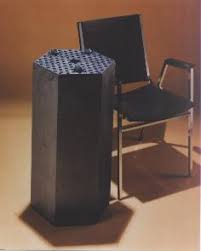
\includegraphics[height=0.6\linewidth]{figs/prismatic.jpeg}
  \caption{Prismatic fuel element block}
  \label{fig:fuela}
\end{subfigure}
\begin{subfigure}{.485\textwidth}
  \centering
  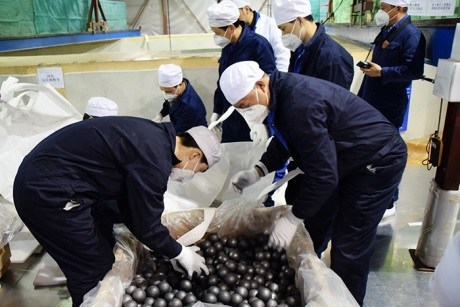
\includegraphics[height=0.6\linewidth]{figs/htr_inspection.jpg}
  \caption{Pebble fuel under inspection}
  \label{fig:fuelb}
\end{subfigure}
\caption{Photos of (a) a prismatic fuel element with a chair for scale \cite{ge_fuel} and (b) pebble fuel elements under inspection \cite{htrpm_fuel}.}
\label{fig:fuel}
\end{figure}

Section \ref{sec:pbr_concept} introduces the salient aspects of the \gls{pbr} design that distinguish the concept from both current commercial designs and the other concepts proposed by the \gls{gif}. The combination of a robust fuel form, passive heat removal systems, and high thermal efficiency make the \gls{pbr} a potentially significant contributor to meeting greenhouse gas emissions targets with improved safety and economic feasibility relative to current commercial reactors.

A notable characteristic of all \glspl{pbr} is a large separation of length scales between the fissile regions in each pebble and the full core. Section \ref{sec:ph_motivation} motivates the role of \gls{th} modeling in reactor analysis with emphasis on the constraints imposed by this large scale separation. Multiscale analysis, a branch of numerical modeling based on decomposing complex systems into separable models for each of the most important characteristic scales, is introduced as one means for achieving fast, design-capable, predictions of \gls{pbr} thermal and flow physics.

After having highlighted important \gls{pbr} \gls{th} phenomena in Section \ref{sec:ph_motivation}, Section \ref{sec:history} sketches a history of the \glspl{pbr} built and operated around the world. Attention is placed on the operational experiences that exemplify the importance of having accurate \gls{th} models of \glspl{pbr} with respect to predicting the thermal and safety design criteria introduced in Section \ref{sec:ph_motivation}. Finally, Section \ref{sec:outline} motivates the methods development and application performed in this dissertation and provides an outline for the remainder of this work.

% TODO: some other kind of big wrap-up here about an opportune moment, etc. Could also be at the very end.

% education plays an important role

% inherent and passive safety issues
% smaller reactors

% not just about climate change, but about helping bring power to all of the world - reference for energy consumption tied to quality of life?

%This is an opportune moment when our shared responsibility for addressing climate change is quite clear.  

%We are accountable to ourselves for delays to action and have a new appreciation for the role of science-based decision making.


%The main driver of climate change is the combustion of fossil fuels, and as such is closely tied to air pollution. The \gls{who} estimates that a million lives could be saved each year worldwide solely due to reductions in air pollution if the goals of the Paris Agreement are met \cite{who_pollution}.

% introduce the use of different coolants - gases and salts, but emphasize that the methods developed in this dissertation apply to both

\section{The Pebble Bed Reactor}
\label{sec:pbr_concept}

% all of the below is great. I don't think you need almost any of it. I guess keep it at this point, but it is way more in depth than what is needed for your dissertation. A two paragraph overview of PBRs followed by a quick overview of modeling methods is really all that's needed to frame your research. This is interesting stuff, but way more than what anyone needs to understand the work you did. 

The defining characteristic of \glspl{pbr} is the use of spherical fuel elements, or ``pebbles.'' Following an early exploratory phase in the 1960s \cite{claxton,hecker}, the multitude of proposed fuel designs have converged to the coated particle form shown in Fig.\ \ref{fig:pbr_fuel}. A typical fuel pebble is 6 \si{\centi\meter} in diameter, slightly smaller than a tennis ball. A central core contains tens of thousands of \glspl{cfp} mixed in graphite. This ``fuel-matrix'' region is protected from erosion by a 0.5 \si{\centi\meter} thick graphite shell on the pebble surface. Each \gls{cfp} is approximately 1 \si{\milli\meter} in diameter and consists of a central kernel of fissile material, typically \gls{uo2} or uranium oxycarbide, surrounded by several layers of structural reinforcement materials \cite{demkowicz, powers}.

\begin{figure}[!h]
\centering
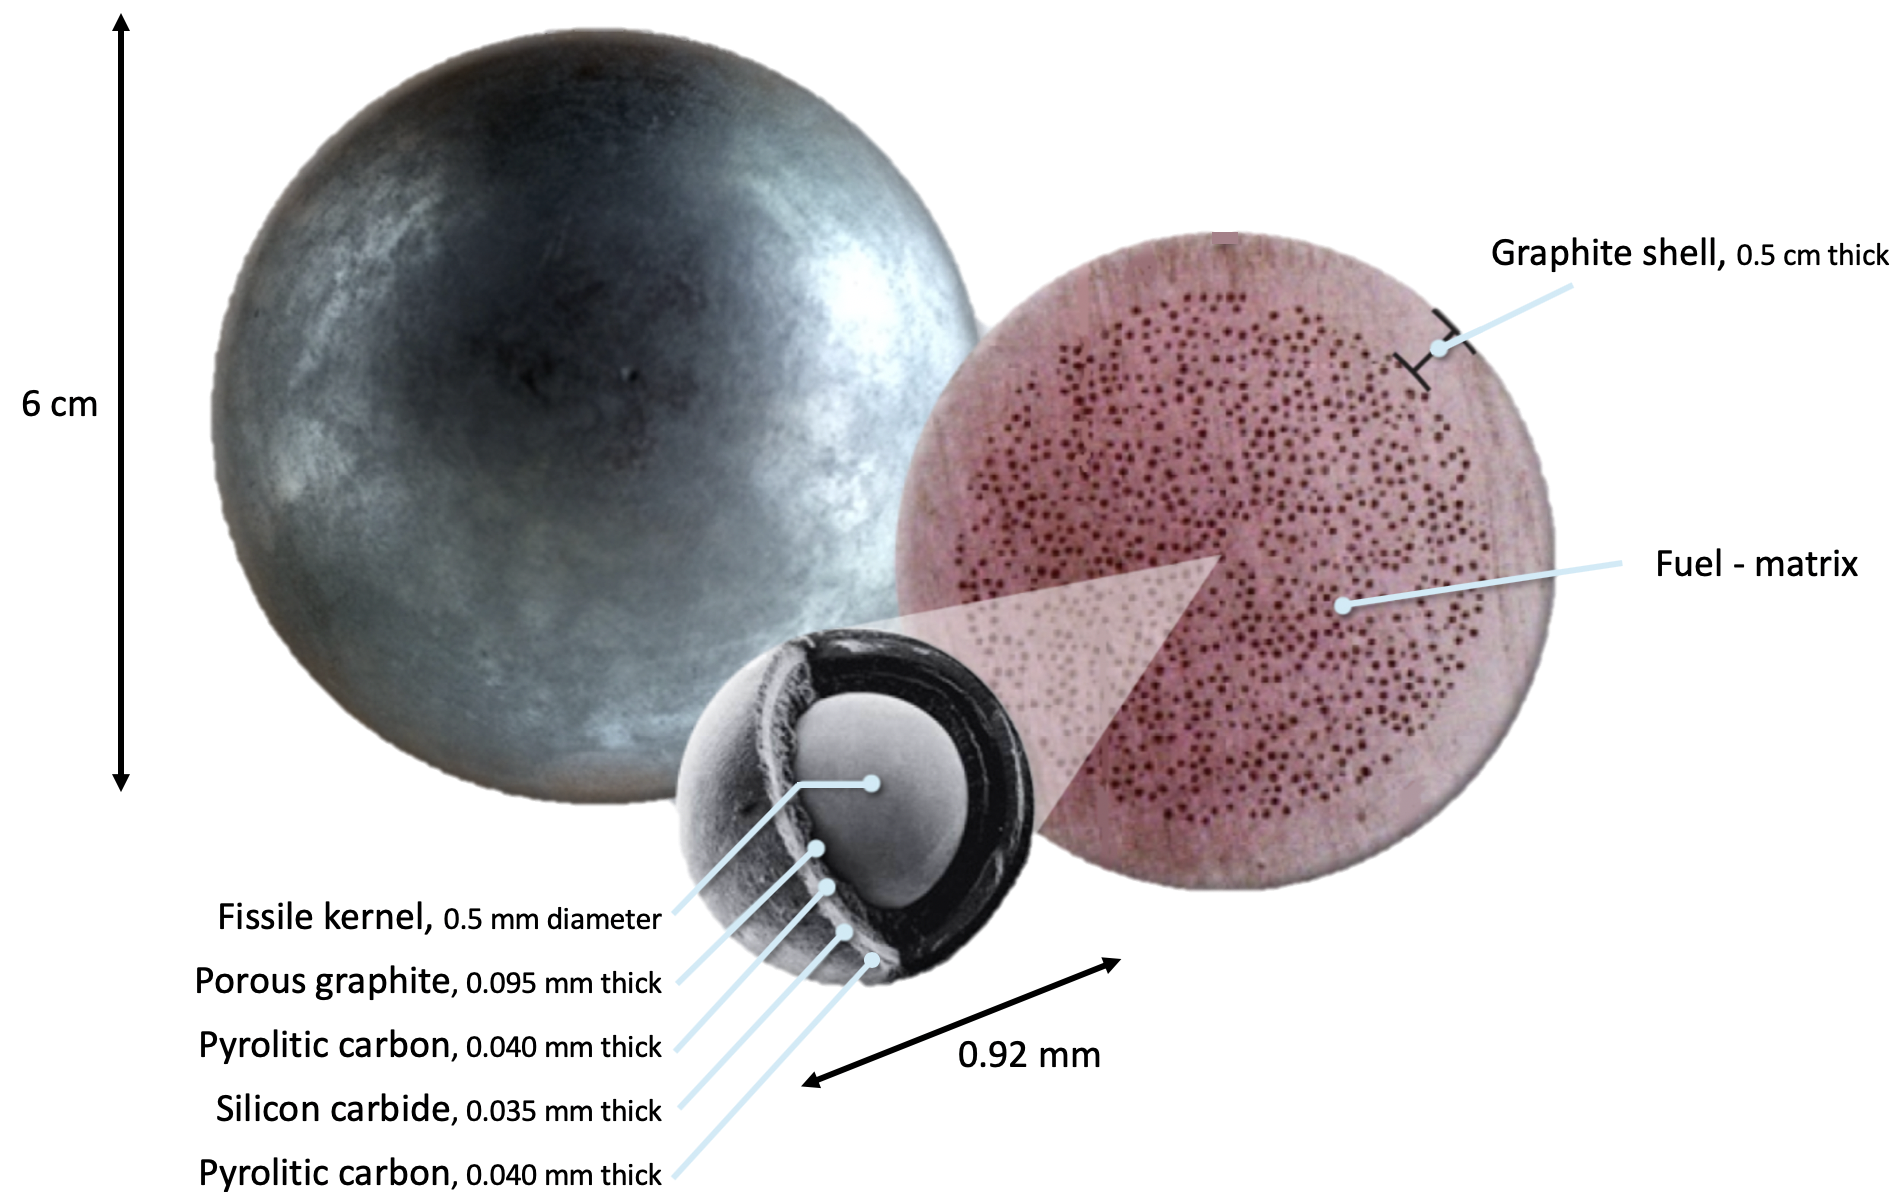
\includegraphics[width=0.6\linewidth]{figs/pbr_fuel.png}
\caption{Typical \gls{pbr} fuel pebble shown from the outside and along a cut-through, with an enlarged \gls{cfp} consisting of five layers (adapted from \cite{x_energy_pebble}).}
\label{fig:pbr_fuel}
\end{figure}

The first of these layers surrounding the kernel is a porous graphite ``buffer'' layer that retains gaseous fission products and accommodates kernel swelling. The \gls{cfp} shown in Fig.\ \ref{fig:pbr_fuel} is more specifically referred to as a \gls{triso} particle due to the use of three additional layers around the buffer\mdash a \gls{sic} layer sandwiched between two \gls{pyc} layers. The \gls{sic} layer is the main pressure vessel for the particle and a diffusion barrier for gaseous and metallic fission products, while the \gls{pyc} layers protect the kernel from damage during the \gls{sic} deposition process and the \gls{sic} from damage during mixing of the particles with the graphite matrix. The robust high-temperature performance of the \gls{triso} particle allows long-term operation at fuel temperatures up to 1250\si{\celsius} and short-term transient operation at fuel temperatures up to 1600\si{\celsius} \cite{nabielek,demkowicz}.

Alternative \gls{cfp} designs exist with different layer structures from the \gls{triso} design show in Fig.\ \ref{fig:pbr_fuel}, though the predominance of the \gls{triso} particle design has led to the generic term ``\gls{cfp}'' being interchanged with the more specific ``\gls{triso} particle'' term in the literature. For generality, ``\gls{cfp}'' is used throughout this dissertation when describing methods that apply equally to other particle designs.

A typical \gls{pbr} core consists of hundreds of thousands of pebbles arranged in a random heap within a cylindrical enclosure formed by loosely-stacked graphite blocks. Fig.\ \ref{fig:corea} shows a plan view of the \gls{htr10} core before loading pebbles and Fig.\ \ref{fig:coreb} shows a photo of the \gls{thtr} bed with control rods inserted directly into the pebble region. Most \glspl{pbr} operate in an online refueling mode, where pebbles are continuously added to the bed, cycled through over the course of several months, and removed at the opposite end. Most reactors operate in a multi-pass scheme where each pebble is re-inserted into the bed two to ten times until the desired burnup has been achieved.

A coolant flows in the interstices between pebbles to remove fission heat. This energy is transported to a power conversion system that generates electricity with a Rankine or Brayton cycle and/or process heat for industrial applications. Upon entering the reactor core, the coolant typically first encounters an open plenum before flowing into the pebble region. In gas-cooled systems, this plenum is present on the top of the bed; pebbles are typically inserted into the core by a free-fall of several meters before hitting the upper surface of the bed. Conversely, the buoyant pebbles used in salt-cooled designs locates the plenum below the bed. In both gas- and salt-cooled designs, the coolant then exits the bed through thousands of ``suction holes'' machined in the reflector blocks that connect the core to the hot legs. The entrance to this outlet plenum geometry is visible in Fig.\ \ref{fig:corea} as the thousands of circular channels machined on the lower angled faces of the bed.

\begin{figure}[!h]
\centering
\begin{subfigure}{.485\textwidth}
  \centering
  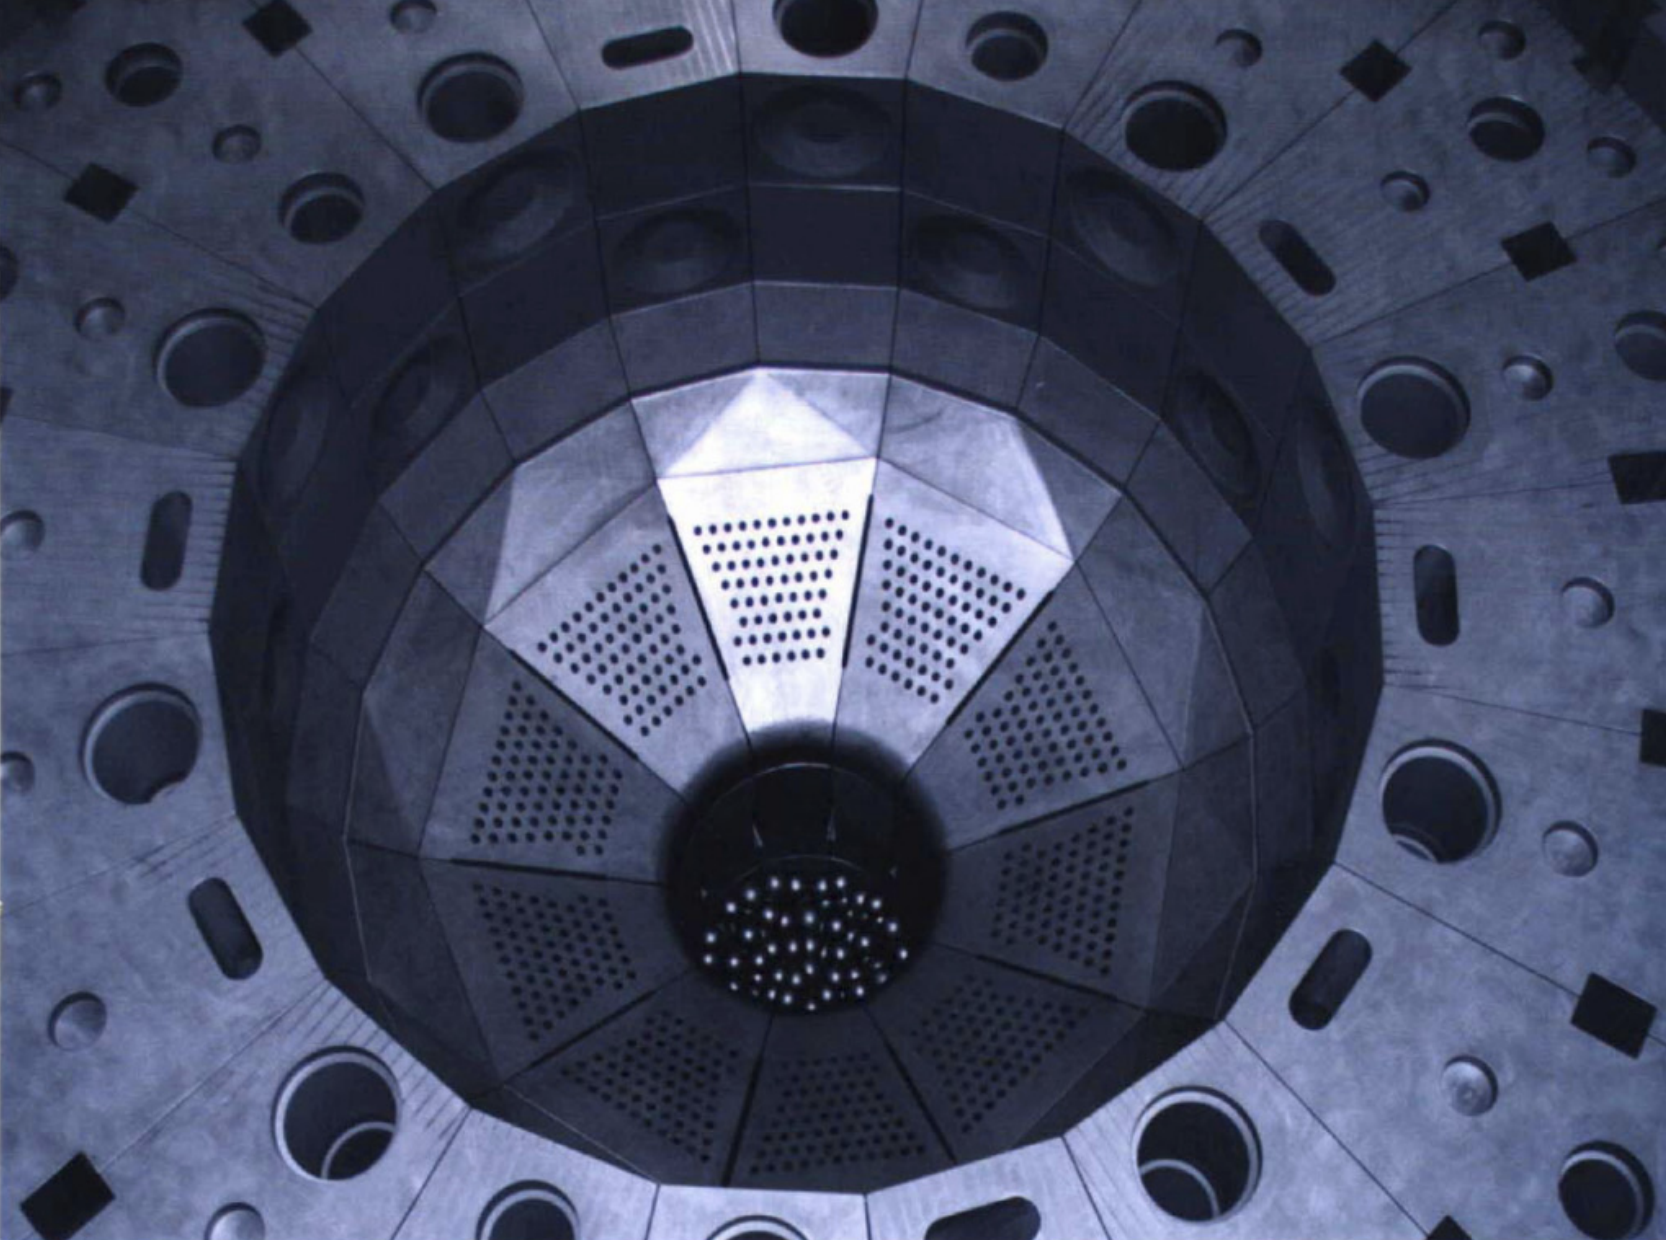
\includegraphics[height=0.5\linewidth]{figs/htr10.png}
  \caption{Plan view of mostly empty HTR-10 core}
  \label{fig:corea}
\end{subfigure}
\begin{subfigure}{.485\textwidth}
  \centering
  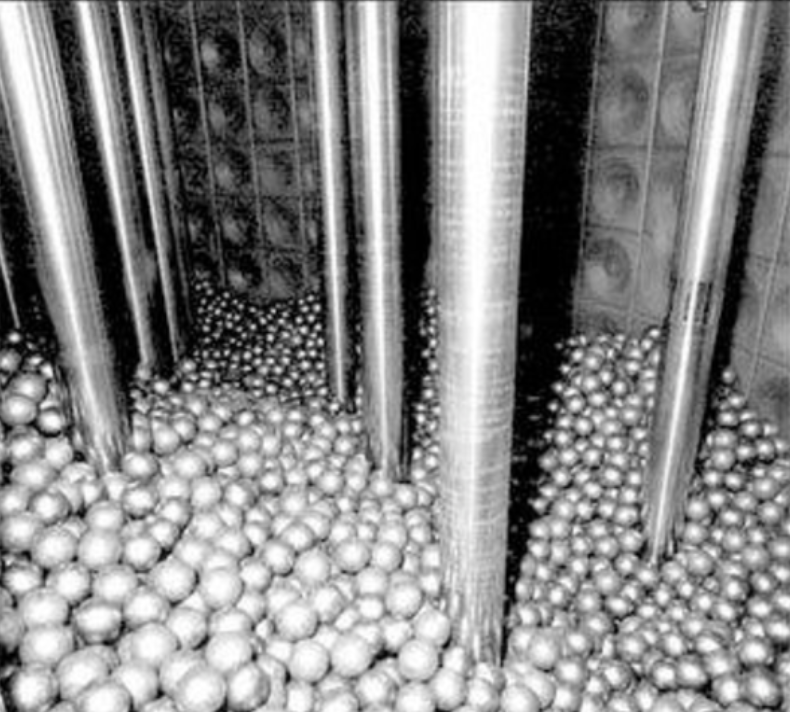
\includegraphics[height=0.5\linewidth]{figs/thtr_core.png}
  \caption{Filled core region of the THTR}
  \label{fig:coreb}
\end{subfigure}
\caption{Photos of the (a) \gls{htr10} core before loading of pebbles \cite{HTGRLessonsLearned} and (b) the \gls{thtr} core with control rods inserted directly into the pebble bed \cite{thtr_core}.}
\label{fig:core}
\end{figure}

In addition to the flow paths through the pebble bed, a number of additional ``bypass'' routes divert coolant from the fuel. In the \gls{htr10} shown in Fig.\ \ref{fig:corea} for example, the outer reflector consists of circular and oblong flow channels that accommodate control rods, backup control systems in the form of loose absorber pebbles, and reflector cooling channels. Coolant may also flow through \si{\milli\meter}-size gaps that form between the reflector blocks due to temperature- and irradiation-induced deformation. Within the bed, pebble ordering near walls also introduces an in-core bypass due to a reduced flow resistance. Both the \gls{htr10} in Fig.\ \ref{fig:corea} and the \gls{thtr} in Fig.\ \ref{fig:coreb} incorporate ``subwoofer''-shaped dimples to disrupt this near-wall pebble alignment.

\glspl{pbr} have a number of economic and safety advantages relative to other reactor concepts. The robust and resilient coated particle fuel form allows long-term operation at high temperature. With proper coolant and structural material selection, \glspl{pbr} may operate at significantly higher coolant temperatures than other reactors. For example, the coolant outlet temperature of the \gls{thtr} was 750\si{\celsius}; about 325\si{\celsius} higher than that of the \glspl{lwr} comprising approximately 96\% of today's commercial reactors \cite{reactor_count}. High temperature operation improves the thermal efficiency of electricity production and expands nuclear power to industrial process heat applications, which represent almost 10\% of total carbon emissions worldwide \cite{friedmann}.

The use of an on-line refueling scheme enables operation with low excess reactivity, which reduces requirements of burnable absorber and control systems and attendant burnup penalties. Provided component accessibility and dose rates permit on-line maintenance, multi-week service and refueling shutdowns may be significantly reduced, increasing reliability and net kWh produced. For multi-pass schemes in particular, frequent opportunities to observe pebble integrity may reduce the coolant source term and lower off-site dose rates. A more fine-grained control of individual pebble burnup may also improve overall fuel utilization relative to fixed-fuel reactors.

Most \gls{pbr} designs use a gaseous coolant such as helium or a liquid coolant with high melting and boiling points such as \gls{flibe} salt. While expensive, non-water coolants eliminate the need to site power plants near large natural or engineered bodies of water and support related environmental impact programs such as stocking programs that replenish fish impinged by water intake pipes \cite{exelon_fish}.
% are all coolants expensive? Also, why does the water requirement go away? The water isn't for the coolant, it's for the heat exchange for the power production. You should still need the water unless you're change the power conversion cycle, right?
More flexible siting constraints may enable non-water cooled systems to provide power in arid regions with lower environmental impact.
% again, I think this is more about how the power conversion system works...
The use of single phase coolants also eliminates many of the operational difficulties associated with two phase liquid-vapor flow such as density-wave oscillations.

The large quantities of high heat capacity graphite in \gls{pbr} cores greatly extends the time scale of thermal transients. Hours or even days may pass before peak temperatures are reached following certain events such as a loss of coolant accident \cite{htrpm,tyobeka}. Slowly-evolving transients that characterize some non-water reactor types mean accidents evolve slowly and therefore provide additional time for human operator response and activities such as equipment repair or substitution should equipment be damaged in an accident.

As with any system designed based on multiple constraints and trade-offs, there are a number of complexities and disadvantages associated with the \gls{pbr} concept. The fuel pebble shown in Fig.\ \ref{fig:pbr_fuel} is approximately 98.2\% graphite by volume, with the remaining 1.8\% occupied by the fissile kernel and \gls{sic}. While large quantities of graphite extend thermal transients, \glspl{pbr} are generally restricted to power densities two to three orders of magnitude lower than other designs such as \glspl{lwr} and \glspl{sfr}. The relatively large reactor vessels of \glspl{pbr} complicate rail transport, contribute significantly to structural material costs, and increase waste volumes.

However, many \gls{pbr} designs refashion power density restrictions to their advantage by employing passive decay heat removal mechanisms that would otherwise be incapable of transporting orders of magnitude higher volumetric heat generation from the core. Power densities are typically low enough that radiation and conduction between touching pebbles, in combination with an ex-vessel water cooling system, is sufficient to remove decay heat in a depressurized \gls{lofc} accident by natural convection cooling. However, the high surface areas required to achieve the needed heat removal rate by the ex-vessel cooling system often impose a leakage penalty.

Low power densities and high fuel fabrication costs both contribute to the use of relatively high fuel enrichments in the range of 9.0 to 19.9\%. Current enrichment facilities are licensed to maximum enrichments of 4.95\%. Without a flourishing \gls{pbr} industry, the economic risks associated with uncertain fuel supplies may lead investors in the advanced nuclear energy sector to pursue non-\gls{pbr} designs. 
% is this because of HALEU? Almost all ARs need HALEU, so that risk applies to almost everyone and is not specific to PBRs. This paragraph either needs more explanation and detail, or should be cut. I'd just cut it. 

The constant abrasion and frictional wear as pebbles move through the bed may generate significant quantities of graphite dust \cite{hecker,moormann}. In gas-cooled designs, solid fission products tend to accumulate in this dust and transport about the primary system in an unpredictable manner, complicating analysis of depressurization events and decommissioning activities due to the mobile and inhalable source term. Instruments and fittings may also not perform as intended in the presence of dust layers. While lubrication in salt coolants may alleviate many operational issues associated with dust generation, additional engineering systems are required to manage this unique solid-solid erosion source term.

In some early fuel designs, the fuel-matrix region was formed as a loose mixture of graphite ``flour'' with \glspl{cfp} to simplify fuel recycling \cite{claxton, hecker}. Reprocessing technologies for graphite-coated \glspl{cfp} today have not progressed beyond the laboratory scale, complicating the ability to close the fuel cycle \cite{moses} but likely reducing the proliferation potential of the \gls{pbr} open fuel cycle.

The high thermal efficiency, passive safety, and high-temperature resilient pebble fuel form of \glspl{pbr} offers great potential to decarbonize the electric and industrial heat sectors. Natural convection decay heat removal and a high thermal inertia contribute to slower transient progression even in the absence of human intervention. However, the low power density, lack of a thriving fuel supply chain or commercial-scale reprocessing technology, and engineering challenges such as dust generation require consideration of these trade-offs in determining the particular markets and missions best suited to commercial deployment. Continued \gls{rd} in the \gls{pbr} space will improve the engineering design of these systems to further enhance the viability of this technology.

% something about small modular reactors?

\subsection{Thermal-Hydraulic Modeling and Simulation}
\label{sec:ph_motivation}

The objective of \gls{th} \gls{ms} of \glspl{pbr} is to vet designs against thermal, mechanical, and radiation limits bounding safe, reliable, and economical operating spaces. Fast-turnaround analysis tools enable more rapid design iterations and scoping studies at significantly lower cost than the long lead-time experimental programs typical of nuclear engineering. As a non-nuclear example, Boeing transitioned from mockup-based experimental programs to heavy reliance on \gls{ms} for the engineering design of the Boeing 777 aircraft. The shift in emphasis from physical experiments to numerical experiments reduced the number of engineering change requests by 90\% and the cycle time for incorporation of a design change by 50\% \cite{boeing}. % more about experiments in nuclear?

For \gls{ms} to be a valuable design tool for reactor development, numerical models must be able to characterize the proximity of the reactor state to the thermal, mechanical, and radiation limits bounding the desired operating space. These limits are expressed in terms of a number of physical metrics that correlate with component damage, worker and civilian dose rates, and degraded economic performance. The ability to effectively cool the fuel is often used as a secondary metric to indicate fuel/core damage and radiation release to the coolant. For the \gls{th} models that are the topic of this dissertation, \gls{ms} tools must be able to accurately predict

\begin{itemize}
\item Maximum coolant outlet temperature, or the highest temperature of structural components that must be maintained below material damage thresholds. The maximum coolant temperature is also correlated to chemical reaction rates such as corrosion.
\item Minimum coolant temperature and freezing-related geometry changes that may reduce fuel cooling.
\item Gradients in the coolant outlet temperature, which result in fluid mixing and cyclic thermal fatigue to structural materials.
\item Maximum fuel temperature, which is correlated to various fuel failure modes that may result in damage and radiation release. Even in the absence of observable damage, the maximum fuel temperature correlates with fission product diffusion coefficients and the coolant source term.
\item Core pressure drop, which is indicative of the pumping power required to cool the core and the feasibility of natural convection decay heat removal in pump loss transients.
\item Fluid-structure interaction and vibration-induced failure modes.
\item Radiation damage and the resulting material dimensional changes and degradation.
\item Radiation activation of the coolant and structural materials.
\item Large-scale structure failure such as pipe breaks.
% add reflector temperature?
\end{itemize}

The physics correlated by these metrics consist of a mixture of core-level phenomena, such as feasibility of natural circulation, and particle-level phenomena, such as fuel particle layer integrity. Recall that a typical \gls{pbr} core consists of a $\backsim$10\si{\meter} tall cylindrical vessel containing hundreds of thousands of \si{\centi\meter}-size fuel pebbles, each of which consists of thousands of \si{\milli\meter}-size \glspl{cfp}. The localization of the heat source to small fissile kernels, the thermal resistance of the \gls{cfp} layers surrounding the fissile kernels, and the core-wide fission power distribution all contribute to significant variation in most \gls{th} phenomena of design interest to \glspl{pbr} over five orders in spatial magnitude. Accurate prediction of the thermal and flow metrics listed above requires model resolution of

\begin{itemize}
\item Heat conduction and material performance in \(\backsim5\times10^9\) fuel particles\hspace{0.01cm}\footnote{Assuming roughly \(5\times10^5\) pebbles and \(1\times10^4\) particles/pebble}; 
\item Intra-pebble heat conduction; inter-pebble conduction and radiation; and pebble-fluid convection and frictional resistance for \(5\times10^5\) pebbles; and
\item Large-scale interactions of the pebble-coolant system with spatially-dependent \gls{bc}, fission power, and material property distributions; reactor control systems; and the \gls{bop} for power generation.
\end{itemize}

\gls{pbr} core analysis is further complicated by its stochastic geometry. Both the \gls{cfp} positions within each pebble and the pebble arrangement within the bed are stochastic. On-line refueling results in a continuous distribution of thermal properties and burnup that are also stochastic. Average packing distributions and granular flow properties are well-quantified for beds of spherical pebbles, while \gls{cfp} positions can usually be approximated with non-overlapping \gls{rsa} methods \cite{jodrey}. However, ensemble averaging is still required to characterize the effect of randomness on the \gls{th} parameters of interest.

\gls{th} models that fully resolve all \glspl{cfp}, pebbles, and the surrounding coolant require \(\backsim10^{12}\) elements in the fluid phase to capture the complex fluid-solid interfaces and boundary layers \cite{wu2010} and \(\backsim10^{15}\) elements in the solid phase to resolve the multiple thin layers on the thousands of \glspl{cfp} in the hundreds of thousands of pebbles \cite{novak_2019}. Furthermore, mesh generation near pebble contact points is often characterized by significant skew that degrades numerical convergence; methods to systematically improve mesh quality in these regions without distorting the porosity remain an open research question \cite{dixon,nijemeisland}.

Most \gls{pbr} beds are surrounded by a graphite block-type reflector that contains flow channels to accommodate control rods, absorber spheres, and coolant flow paths. Horizontal and vertical gaps with widths on the order of \(10^{-3}\) \si{\meter} form between the blocks as a function of irradiation and temperature \cite{guo_2018,liu_sas}. The engineered flow channels, in combination with these gaps, permit bypass flow paths that simultaneously cool the reflector and core externals while diverting coolant from the fuel. These reflector bypass flows therefore have important effects on thermal stresses, overall component lifetime, and uniformity of outlet temperatures, and must be considered in core \gls{th} analysis \cite{guo_2018,anderson}. However, coupling the reflector bypass flows to a bed \gls{th} model greatly increases the size of the simulation domain and requires judicious mesh generation for a geometry consisting of a mix of very thin gaps and comparatively large engineered channels.

Such ``high-resolution'' models, which fully resolve all geometric scales in the pebble bed and reflectors, are intractable for the fast-turnaround calculations needed for routine reactor design and analysis. The ``everyday'' computing resources available to regulatory agencies and the nuclear power industry are typically single-user, multi-core, workstations sized to perform tens to hundreds of design iterations per day \cite{nrc_nonlwr}. While high-resolution models are invaluable for benchmarking lower-resolution tools, generating closures, and exploring fine-scale phenomena, supercomputing resources currently limit these calculations to homogeneous pebble interiors in either a random heap of several hundred pebbles or a regular lattice with symmetry conditions\mdash far short of the hundreds of thousands of pebbles, and their heterogeneous interiors, constituting a \gls{pbr} core \cite{calis,zhang2016,baker_2010,alkhalaf,guardo,gunjal}.

Multiscale analysis is a branch of applied mathematics that is based on decomposing a complex system into a number of important temporal and/or spatial length scales, each described by different models, that are then aggregated together to obtain a representative physics solution over many orders of magnitude in time and/or space. Provided the models for each characteristic scale are sufficiently simple, the computational cost of a multiscale decomposition may be orders of magnitude lower than a fully-resolved model. 

This dissertation develops and applies multiscale models to \gls{th} analysis of single-phase \glspl{pbr}. These multidimensional models are of ``intermediate'' fidelity\mdash they are lower in resolution than the fully-resolved models described in the preceding paragraphs, but higher in resolution than the 1-D flow network models used for loop analysis or the pseudo 3-D subchannel methods used for primarily unidirectional flows. Before outlining the work performed in this dissertation in Section \ref{sec:outline}, Section \ref{sec:history} provides a brief history of \gls{pbr} \gls{rd} around the world with emphasis on operating experiences that highlight the importance of having accurate models of \gls{pbr} \gls{th}. 

\subsection{A Brief History in the Context of Thermal Analysis}
\label{sec:history}

This section traces a brief history of the design, development, and operation of \glspl{pbr} around the world to demonstrate the relevance of the methods developed in this dissertation to predicting complex and engineering-significant phenomena in \glspl{pbr}. For brevity, emphasis is placed on programs that resulted in construction and operation of a \gls{pbr} or that are currently engaged in doing so. The reader is referred to the literature for more comprehensive chronologies \cite{claxton,thomas}. And rather than attempt a complete technical description of each \gls{pbr} design, attention is focused on the operational experience related to the thermal safety and reliability criteria introduced in Section \ref{sec:ph_motivation}. This section concludes with an in-exhaustive survey of several concepts under development in the United States and abroad to highlight the wide variety of systems that multiscale models must consider.

In the late 1950s, a group of 15 utility and power supply companies united as \gls{avr} GmbH with German government support to construct the first \gls{pbr}\mdash a 15 MWe, helium-cooled, reactor in J{\"u}lich, Germany \cite{hecker,oehme,nrc_avr,moormann}. The purpose of this project was to explore the \gls{pbr} concept and its technical feasibility for electricity and process heat applications. This reactor, referred to as the \gls{avr}, achieved first criticality in 1966 and operated for over 20 years, providing invaluable technical experience and demonstrating the feasibility of many aspects of the {pbr} design such as fuel handling systems, \gls{bop} components, and gas purification processes. Many key safety aspects of \gls{pbr} designs were verified; a series of progressively evolving \gls{cfp} fuel forms exhibited excellent fission product retention at high temperatures, while \gls{lofc} experiments proved natural circulation to be capable of safely removing decay heat. The \gls{avr} also set the world record for highest sustained outlet temperature of a nuclear reactor\mdash990\si{\celsius}.

One of the more well-known experiments conducted in the \gls{avr} involved the measurement of bed temperatures during steady-state operation. Due to the difficulty of obtaining temperature readings within a moving, random heap of pebbles, 120 non-fissile instrumented pebbles were loaded into the bed, cycled through, and removed after a single pass. Fig.\ \ref{fig:avr_melt} shows a picture of one of these instrumented pebbles; a center plug contains a wire with a known melting temperature. With 20 different wire materials and two load locations, a very coarse temperature map was obtained. The majority of pebbles indicated temperatures up to 200\si{\celsius} higher than permitted in the reactor license \cite{sobes,moormann}. And, depending on location, between 7 and 31\% of the pebbles exceeded the maximum wire melting temperature of 1280\si{\celsius}; coarse estimates suggest these pebbles exceeded allowable temperatures by as much as 240 to 340 K. Decades later, improved computational models and an improved understanding of \gls{pbr} \gls{th} suggests that a large contributor to these high temperatures in the \gls{avr} was neglecting bypass flow through control rod channels and gaps formed between the carbon insulation and the reactor shroud \cite{viljoen}, though it is likely that hot spot formation also played an important role \cite{moormann}.

\begin{figure}[!h]
\centering
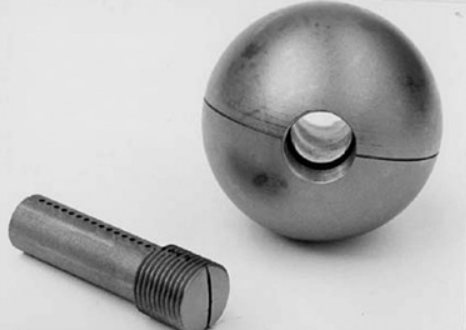
\includegraphics[width=0.4\linewidth]{figs/avr_melt_wire.png}
\caption{Non-fissile instrumented melt wire pebble for measuring temperatures in the \gls{avr}.}
\label{fig:avr_melt}
\end{figure}

Soon after the \gls{avr} reached first criticality, design of the 300 MWe \gls{thtr} commenced in Germany with a mix of government and utility funding \cite{oehme,thtr_1990,hecker,hofmann}. The purpose of this follow-on design was to further refine the \gls{pbr} technology and provide a bridge from the small \gls{avr} to subsequent commercial plants. The \gls{thtr} design was largely based on scaling up the \gls{avr} design, with modifications to enable a significantly larger core such as a faster fuel handling system, addition of control rod insertion points directly in the bed, and downward-flowing coolant to limit power density reductions due to levitating pebbles \cite{claxton}. The evolution of regulatory requirements during the construction phase extended the construction period by a factor of three and the cost by a factor of five. The \gls{thtr} achieved first criticality in 1983 and began power operation in 1985. 

Like the \gls{avr}, reactor operation was considered quite successful, though a number of operational challenges emerged. At high coolant flow rates, bypass flows through discharge tubes prevented pebble defueling. Further, the graphite shells on about 1.5\% of the pebbles were damaged from frequent and deep insertion of control rods into the bed and high compressive forces. Experiments in air failed to predict the order of magnitude higher graphite friction coefficient in high temperature and pressure helium environments. Failure of insulation attachment bolts in the hot gas ducts near the bed exit can likely be attributed to excessive core outlet temperature gradients and the ensuring thermal stresses \cite{moormann}. Like the \gls{avr}, the \gls{thtr} significantly underpredicted the bypass flow through reflectors; an initial estimate of 7\% bypass was refined to 18\% following plant measurements. While this larger bypass has been attributed to 10\% higher fuel temperatures than initially predicted, the significantly lower operating temperature of the \gls{thtr} as compared to the \gls{avr} maintained temperatures within the licensed space.

While generally considered an engineering success, the engineering partners involved in the \gls{thtr} project decided to shut down the reactor after only three years of power operation due to financial risks related to an uncertain fuel supply, an incomplete spent fuel disposal plan, and unknown future licensing criteria. At the instigation of the German government, Siemens and the successor company to the merging of entities involved in the \gls{thtr} united as a new company named HTR GmbH which later developed a commercial 200 MW$_\text{th}$, helium-cooled, \gls{pbr} design known as the HTR-Modul. Following the fall of the Berlin wall in 1989, the ongoing negotiations between HTR GmbH, the East German government, and the \gls{ussr} for purchase of several HTR-Modul plants ceased. No further \glspl{pbr} have been constructed in Germany.

In 1999, the South African power utility Eskom obtained a non-exclusive license from HTR GmbH to further develop gas-cooled \gls{pbr} technology. With significant support from the South African government, \gls{pbmr} Ltd. was formed and a large engineering program focused on extending the HTR-Module design to a 400 MW$_\text{th}$, direct gas cycle, multi-module plant design referred to as the \gls{pbmr400} \cite{thomas, koster}. In 2010, the South African government withdrew financial support due to an inability to attract customers and foreign investment to the project. Engineering challenges such as insufficient experience in helium-driven gas turbines, which were misleadingly being referred to as ``standard'' Brayton cycles and thus implying a more technically ready power cycle, contributed to time overruns. While no demonstration plant was ever built, a significant share of the fundamental and engineering research in \gls{pbr} \gls{th} was performed by \gls{pbmr} Ltd.

Roughly contemporary with the German reactor operation and the South African efforts, China commenced a \gls{pbr} program to investigate applications in clean energy and hydrogen fuel cell process heat. About a decade after the \gls{avr} and \gls{thtr} were shut down, construction was completed on a 10 MW$_\text{th}$, helium-cooled, \gls{pbr} by the \gls{inet} at Tsinghua University; first criticality was achieved in 2000 \cite{gao,chen_htr,xu_htr}. This reactor, known as the \gls{htr10}, is largely based on the German \gls{pbr} designs. A number of safety demonstration tests centered on \gls{atws}, \gls{lofc}, and \gls{loop} events have continued to prove the inherent safety features of gas-cooled \glspl{pbr} first demonstrated in the German reactors.

Building off the success of the \gls{htr10}, two Chinese utilities and \gls{inet} established a project to build a scaled-up demonstration plant at Shidao Bay in Shandong Province \cite{xu_htr,htrpm,htrpm_website}. This reactor, known as the \gls{htrpm}, is a 250 MW$_\text{th}$, helium-cooled, design that will likely be the first Generation IV reactor in operation. The reactor vessel head was installed in late 2017, and construction continues through 2020 \cite{htrpm_2020}. While the \gls{htrpm} is largely based on scaling up the \gls{htr10} design, a significant difference from the draft \gls{htrpm} design is the omission of a central column of graphite pebbles that cosntrainted the power-generating region into an annulus. Early iterations of the \gls{pbmr400} design also included a central graphite pebble column \cite{koster}; for both reactors, the unexpectedly high bypass flows through this column led to removal from subsequent design revisions.

In 2011, the \gls{cas} initiated a research program focused on salt-cooled \gls{pbr} technology to explore industrial heat applications and incrementally develop supporting technologies for liquid-fueled \glspl{msr} \cite{dai}. The first stages of the project involve the construction of a 10 MW$_\text{th}$, \gls{flibe}-cooled, \gls{pbr}referred to as the \gls{tmsrsf1} that will be the first salt-cooled \gls{pbr} in the world. 

Today, a number of \gls{pbr} concepts are being pursued by startup companies in the United States and research institutions worldwide. X-Energy, based in Maryland, is developing a 200 MW$_\text{th}$, helium-cooled, \gls{pbr} design and the associated fuel fabrication capabilities with a target market introduction in 2030 \cite{x_energy}. Kairos Power, based in California, is developing a 311 MW$_\text{th}$, \gls{flibe}-cooled, \gls{pbr} design that leverages a long history of salt-cooled \gls{pbr} research and technology development at \gls{ucb}, \gls{mit}, \gls{uw}, and a number of other Universities \cite{kairos}. The National Nuclear Energy Agency of Indonesia has expressed interest in building a small, helium-cooled, \gls{pbr} with a design similar to the Chinese \gls{htr10} \cite{liem}. 

While most fluidized bed designs are based on molten salt coolants, a fluidized design with water coolant has also been proposed. One particular design suspends a large ``clump'' of approximately 1\si{\centi\meter} diameter pebbles in upwards-flowing water, where the axial density variation of the coolant ensures spatial stability of the bed \cite{sefidvash, sefidvash_1996}. The pebbles may be solid \gls{uo2} clad in zircaloy or miniaturized versions of \gls{htgr} pebble fuels with the graphite shell replaced by \gls{sic}. This water-cooled fluidized bed concept has recently been modified to a fixed bed structure with pebbles as small as 2 \si{\milli\meter} in diameter by researchers at Xi'an Jiaotong University \cite{cai,li_pbwr}.

There a number of important takeaways from this historical survey. First, accurate \gls{th} models are essential to ensuring safe and reliable operation and meeting the conditions set in operating licenses. Deficiencies in early \gls{th} models of \glspl{pbr} failed to accurately characterize bypass flow in the \gls{avr} and \gls{thtr}, leading to excessively high fuel temperatures in the \gls{avr} with significant implications on fuel integrity given the already high coolant operating temperature. Unexpectedly large gradients in outlet temperature in the \gls{thtr} may have contributed to stresses and bolt failure at the core outlet.

Second, computational models are an indispensable tool for reactor design. Both the \gls{pbmr400} and \gls{htrpm} designs underwent significant modifications once numerical predictions showed excessively high bypass flows through a pebble-type center reflector. Reaching the same conclusion through an experimental program would have consumed far greater time and investment than the use of a computational model.

And finally, the viability of a reactor technology is equally dependent on the regulatory framework and supply chain as on the design's technical merits. This dissertation focuses exclusively on models to assess the physical characteristics of a \gls{pbr} design, and it is important to recognize that this work is just one portion of the larger nuclear development life cycle\mdash technical design, licensing, construction, operation, and decommissioning. 

\section{Objectives and Outline of this Dissertation}
\label{sec:outline}

The objective of this dissertation is to develop and apply multiscale models to the thermal and flow analysis of \glspl{pbr} to 1)~expand the physics capabilities and resolution available to the \gls{pbr} industry, 2)~provide recommendations on the use of multiscale analysis for \glspl{pbr}, and 3)~demonstrate the use of these models for engineering design and analysis by exploring the \gls{th} characteristics of a novel salt-cooled \gls{pbr} concept.

The multiscale models developed in this dissertation are based on decomposing the \gls{pbr} geometry into three length scales\mdash

\begin{enumerate}
\item The microscale, defined over a single \gls{cfp};
\item The mesoscale, defined over a single fuel pebble; and
\item The macroscale, defined over the entire reactor core, which encompasses the pebble bed, reflectors, and structural materials.
\end{enumerate}

In Chapter \ref{sec:PhysicalModels}, the models for each of these length scales are derived. Spatial homogenization of the Navier-Stokes equations with conjugate heat transfer, often referred to as the ``porous media'' approach, is used to describe the macroscale. Two different methods are considered for the meso and micro length scales\mdash the first is a simple volume-preserving homogenization that reduces a 3-D heterogeneous solid to a 1-D set of conducting layers. The second is a linear superposition technique that adjusts a long-wavelength mesoscale model with a microscale correction for each \gls{cfp}. 

The homogenization inherent in these scale models relies upon a number of closures to account for local variations on mean properties. Sections \ref{sec:Closures} and \ref{sec:ClosuresMesoMicro} reviews the closures used in subsequent chapters. By including thermal dispersion and the combined effects of inter-pebble conduction and radiation, these models consider additional physics typically neglected in salt-cooled \gls{pbr} analysis \cite{xin_wang_thesis,scarlat} but that represent important heat transfer processes, especially at high temperature. 

Motivated by a need for tight in-memory multiphysics coupling, unstructured 3-D meshes, and open source software longevity, Chapter \ref{sec:ph} describes the implementation of the physical models derived in Chapter \ref{sec:PhysicalModels} in a new software application. This application, named Pronghorn, is a continuous \gls{fem} tool built on the open source \gls{moose} that leverages state-of-the-art numerical methods, nonlinear solvers, and meshing tools to achieve high-performance physics simulations with high quality software engineering practices. The \gls{fe} spatial discretization, software implementation, nonlinear solvers, and stabilization schemes are described. By assuming that the fine length scales are periodic with respect to the coarser length scales, scale coupling is achieved through a Picard iteration with in-memory feedback through \glspl{bc} and source terms. 

The use of computational models to predict reactor response requires high quality software and a strong \gls{vv} base. Chapter \ref{sec:vv} presents four verification tests of the multiscale models to support application to \glspl{pbr} in Chapters \ref{sec:sana} and \ref{sec:pbfhr}. Of particular interest to the use of these multiscale models for both the porous bed and open plena in \glspl{pbr}, numerical benchmarks for thermally-driven, open natural convection flow and inviscid cylinder flow are shown. 

In Chapter \ref{sec:sana}, the multiscale models are applied to the SANA facility, a scaled experiment built and operated in Germany in the mid 1990s that models depressurized conduction cool-down of gas-cooled \glspl{pbr}. By simulating 52 different experiments with a variety of pebble designs, coolants, and heater arrangements, a wealth of validation data demonstrates a mean error of 22.6\si{\celsius} and a standard deviation of 54.6\si{\celsius} in multiscale predictions of solid temperature. A code-to-code comparison demonstrates slightly lower error and standard deviation relative to two other existing \gls{pbr} simulation tools, with the additional benefit of unstructured meshing capabilities and flexible in-memory data communication with other \gls{moose} applications.

By investigating the error as a function of position within the bed, it is found that the standard deviation decreases with distance from both radial and axial walls, while the error only decreases with distance from radial walls. These observations highlight the need for anisotropic drag and heat transfer closures for near-wall regions, which are all but absent from the porous media literature. The primarily radial temperature gradient also suggests that more accurate thermal predictions can be achieved via improved heat flux \glspl{bc}. Model closures are then individually varied relative to a baseline set to show the importance of closure selection in gas-cooled \gls{pbr} analysis. The solid temperature is sensitive to the porosity and near-wall treatment of the solid effective thermal conductivity. Future experimental programs may choose to emphasize closure development in the areas of heat flux \glspl{bc}, near-wall effective solid conductivity, and axial porosity distributions to improve multiscale models of gas-cooled \glspl{pbr}.

Chapter \ref{sec:pbfhr} then applies the multiscale models to thermal and flow analysis of the Mark-1 \gls{pbfhr}, a \gls{flibe}-cooled reactor developed by the Nuclear Engineering department at \gls{ucb} and a number of other Universities. The objective of this concluding chapter is to demonstrate the use of the models developed, verified, and validated in previous chapters to full-core reactor design and analysis. This particular reactor concept is selected due to an unconventional reflector block design, a unique ``thermally-thin'' pebble fuel-matrix region, and non-uniform flow \glspl{bc} that highlight the new capabilities enabled by this dissertation for \gls{pbr} industrial analysis.

The two fuel models developed in Chapter \ref{sec:PhysicalModels} are compared against reference, fully-resolved, Mark-1 \gls{pbfhr} fuel pebbles in Section \ref{sec:meso_fhr} for a wide range in thermal conditions. The especially thin fuel-matrix annulus is poorly represented by the homogeneous layer multiscale model used in a previous dissertation on this subject \cite{xin_wang_thesis}, while the linear superposition technique predicts temperatures remarkably well. While average and maximum temperatures are predicted to within about 10\si{\celsius} for the linear superposition technique over the entire range in thermal conditions considered, the homogeneous layers approach is at times characterized by errors in excess of 200\si{\celsius}.

In Section \ref{sec:bypass}, resolved COMSOL \gls{cfd} simulations of the \gls{pbfhr} reflector blocks are used to correlate anisotropic friction factor models as a function of Reynolds number. By considering several different block geometries, the strong effect of reflector drag on irradiation- and temperature-induced deformation, as well as flow direction, is demonstrated.

Section \ref{sec:core} then combines the macroscale model \gls{vv} in Chapters \ref{sec:vv} and \ref{sec:sana} with the pebble model verification in Section \ref{sec:meso_fhr} and reflector block drag closure generation in Section \ref{sec:bypass} to full-core analysis of the Mark-1 \gls{pbfhr}. A parametric study varying the reflector block gap distribution and the inflow \gls{bc} demonstrates that 1)~the inflow \gls{bc} has a significant effect on the core bypass fraction and outlet fluid temperature distribution, 2)~the bypass fraction must be considered in conjunction with the inflow \gls{bc} when assessing proximity of the reactor design to fluid temperature design limits, and 3)~the bypass fraction is a strong function of the reflector block gap distribution. A modified block design at the entrance and exit of the bed is identified as a possible future development area to further reduce the core bypass.

Based on balancing a number of core thermal design criteria, Section \ref{sec:depth} predicts fuel and reflector temperatures for a fixed inflow \gls{bc}. The primary effect of the core bypass is to uniformly raise core temperatures; when normalized to a common maximum fluid temperature, solid temperatures are nearly identical among the various reflector block gap distributions considered. The maximum kernel temperature is approximately 93\si{\celsius} higher than the maximum fluid temperature, which remains far below the fuel failure limits of \gls{triso} particles. Additional thermal design activities may be performed in the future to further increase the margin between the average fluid outlet temperature and the 730\si{\celsius} limit typically imposed for Hastelloy N \cite{xiao}.

Finally, Chapter \ref{sec:conclusions} summarizes the major findings of the analyses in Chapters \ref{sec:vv}--\ref{sec:pbfhr} and provides guidance on the future application of multiscale modeling to \glspl{pbr}. This dissertation focuses exclusively on \gls{th} modeling, which is just one component of a comprehensive reactor analysis framework considering neutron transport, materials performance, structural mechanics, and many other physics domains. By developing high-quality predictive models capable of rapid \gls{th} design and analysis, this work plugs into the larger community developing computational tools to enable the contribution of Generation-IV reactors to a clean energy economy.

% TODO: revisit this conclusion after getting comments back from people

% methods for single-phase PBRs, less distinction between their engineering differences, but rather the modeling challenges that they all share.

\chapter{Multiscale Models for Pebble Bed Reactors}
\label{sec:PhysicalModels}

Many systems exhibit wide ranges in temporal and/or spatial scales such that the use of models applicable to the ``smallest common denominator'' scale for all length scales are computationally impractical. Examples of such systems include Earth's climate, drugs targeting cancer cell growth, fluid flow, and \glspl{pbr}. Multiscale analysis is based on decomposing a complex system into a number of important temporal and spatial length scales, each described by different models, that are aggregated together in an intelligent manner to obtain a representative solution for the relevant physical phenomena on all length scales. The underlying motivation is to enable comprehensive physics predictions at significantly reduced computational cost relative to fine-scale modeling of all scales. 

\glspl{pbr} are naturally described in terms of three length scales\mdash 1)~the macroscale, defined over the entire reactor core, which encompasses the pebble bed, reflectors, and structural materials; 2)~the mesoscale, defined over a single pebble; and 3)~the microscale, defined over a single fuel particle. Fig.\ \ref{fig:multiscale} depicts these three length scales for the pebble bed region. For a typical \gls{pbr}, the characteristic macro, meso, and micro length scales are approximately \(5\times10^0\) m, \(5\times10^{-2}\) m, and \(1\times10^{-3}\) m, respectively, such that the mesoscale is approximately 100 times smaller than the macroscale and the microscale is approximately 50 times smaller than the mesoscale. 

By assuming fine length scales are periodic with respect to coarse length scales, \glspl{bc} from the coarser-length solution are applied to finer-scale models to obtain representative thermal and flow predictions for all length scales. This section describes the multiscale modeling approach developed in this dissertation in terms of the three length scales shown in Fig.\ \ref{fig:multiscale}. Section \ref{sec:macro_deriv} discusses the macroscale model, while Section \ref{sec:mesomicro} discusses the meso and micro scale models. Finally, Section \ref{sec:MacroAssumptions} elaborates on the most important limitations, assumptions, and knowledge gaps in this multiscale application to \glspl{pbr}. The interested reader will find detailed derivations and additional discussion in the theory manual accompanying the software implementation of these concepts \cite{novak_manual}. 

\begin{figure}[!h]
\centering
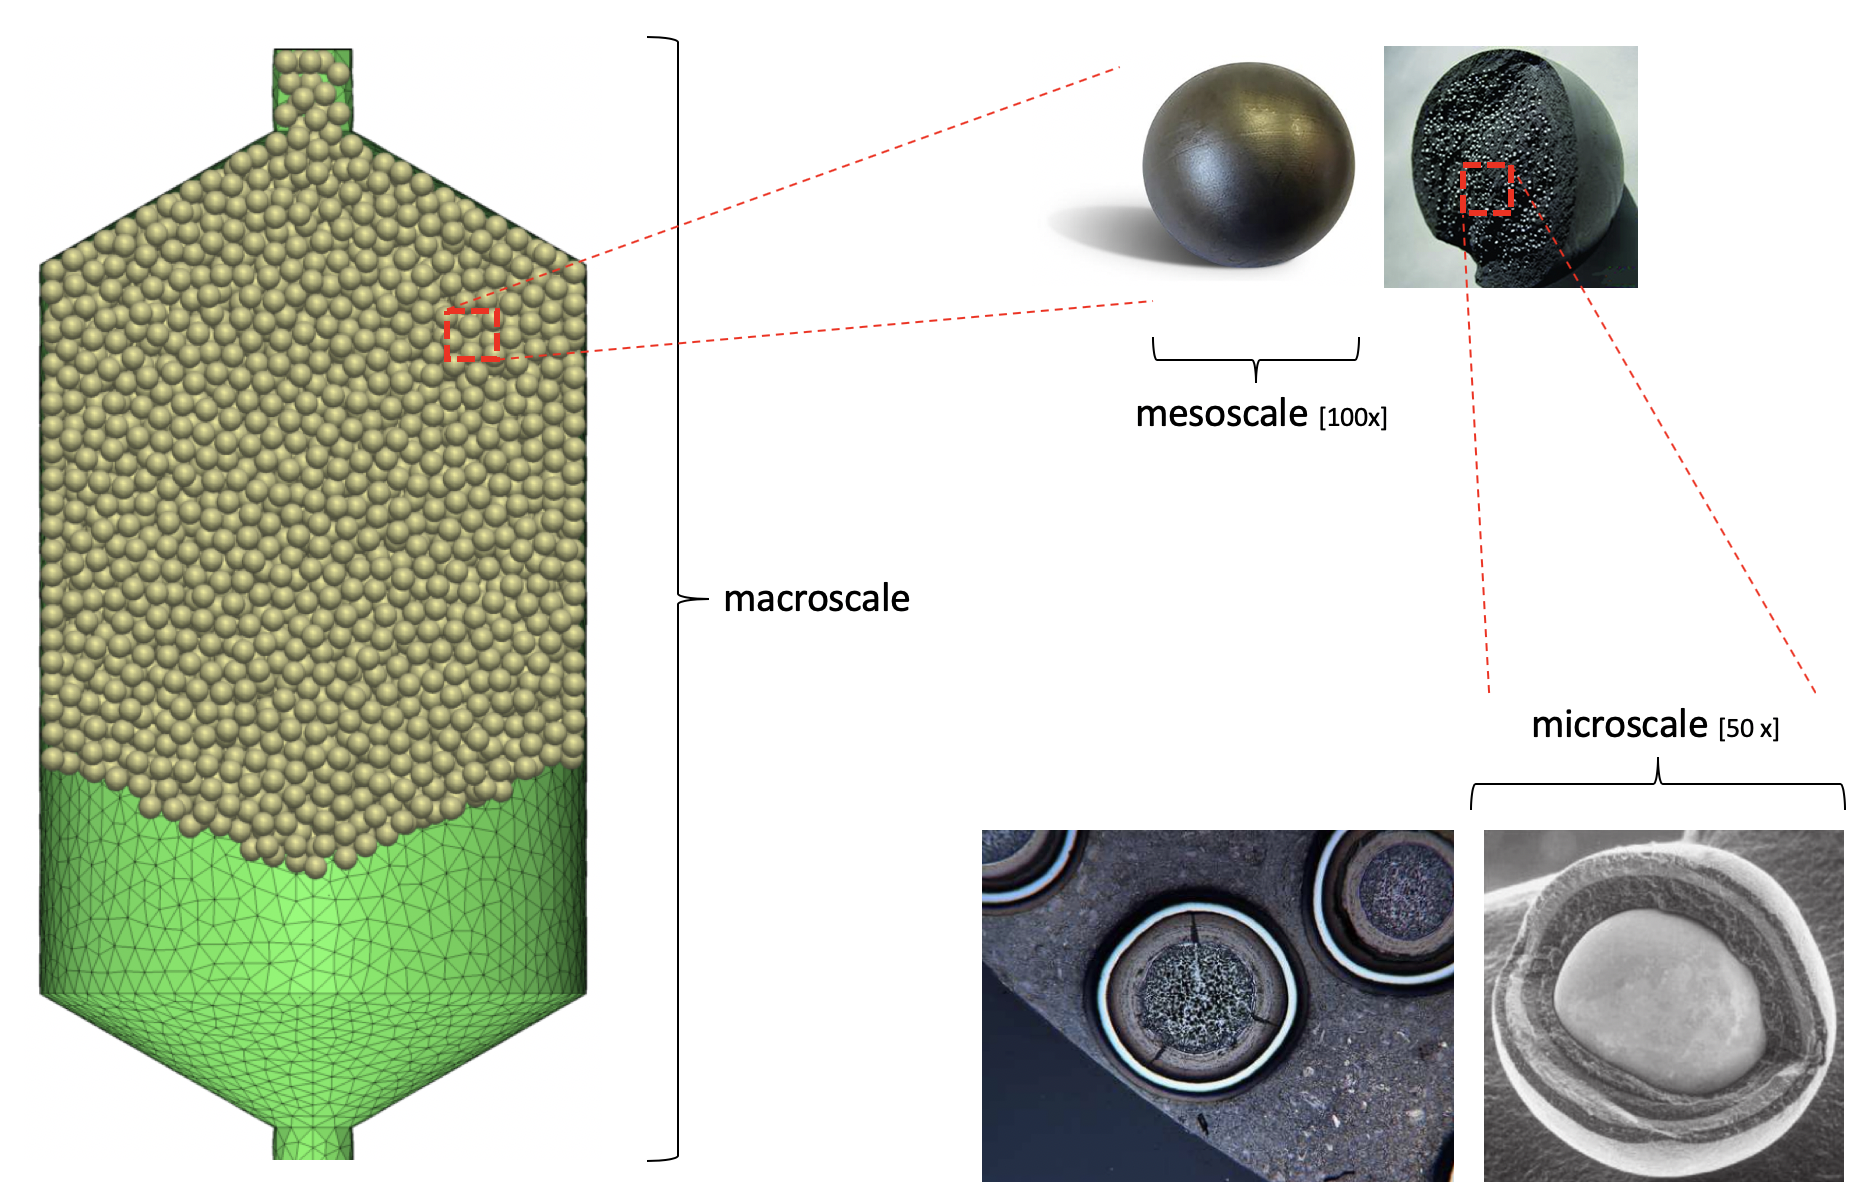
\includegraphics[width=0.9\linewidth]{figs/multiscale_pbr.png}
\caption{Decomposition of a \gls{pbr} into three length scales (adapted from \cite{aufiero_2016,pebble_cut,pebble_uncut,triso_closeup,hales}).}
\label{fig:multiscale}
\end{figure}

\section{Macroscale Model}
\label{sec:macro_deriv}

The macro length scale characterizes the two-phase mixture of fluid coolant with solid pebbles and reflector blocks. On a spatial scale on the order of the pore size between pebbles or the gap size between reflector blocks, the flow characteristics are highly irregular. For example, turbulent intensities along pipe centerlines are commonly on the order of 5\%, but experiments in pebble lattices show turbulent intensities as high as 50\% in void centers \cite{mickley}. 

However, on a scale encompassing small groups of pebbles or blocks, averaged flow properties are regular and predictable. Fluid flow and heat transfer through a two-phase mixture of fluid and solid phases is governed by the Navier-Stokes equations with conjugate heat transfer\hspace{0.02cm}\footnote{``Conjugate'' heat transfer refers to heat transfer between fluids and solids.}. Spatial homogenization of these governing equations over a length scale larger than the characteristic pore size captures physical phenomena that vary on the macroscale at the expense of averaging fine-scale physics through model closures. Spatial homogenization over multiple phases is often referred to as the ``porous media'' method due to its connections to Henry Darcy's study of water flow through sand in Dijon, France \cite{darcy}.

A porous media in general refers to a solid matrix with interconnected voids filled with gas and/or liquid. A diverse set of systems have been modeled as porous media, ranging from the flow of water through permeable subterranean rock to conductive heat flow through composite materials \cite{diersch}. Within the nuclear engineering field, porous media models are commonly applied to flow and heat transfer in tube-in-shell heat exchangers \cite{ge_prhr}, quenched corium heaps \cite{magallon,raverdy}, tritium breeder blankets in fusion reactors \cite{xu_cfetr,zhang2016,guo2006}, and pin-fueled fission reactors \cite{zarifi}. For application to \glspl{pbr}, the solid matrix is interpreted as the stacked reflector blocks and randomly heaped pebbles, while the interconnected voids correspond to the fluid interstices between the solids and the machined flow channels within blocks. The solid phase in a porous media is often referred to as ``particles;'' to avoid confusion with the particles within \gls{pbr} fuels, ``pebbles'' is used to refer to the solid phase on the macroscale, while ``particles'' is used to refer to the \glspl{cfp}.

This section presents the derivation of the spatially homogenized Navier-Stokes equations with conjugate heat transfer. While ``Navier-Stokes'' strictly refers to the momentum conservation equations for a Newtonian fluid, this work follows a looser convention of referring to the set of coupled mass, momentum, and energy equations together as the Navier-Stokes equations. This is performed to differentiate from a different set of coupled equations referred to as the ``friction-dominated'' equations derived later that differ from the Navier-Stokes equation set in the mass, momentum, and energy equations.

A nondimensional analysis in Section \ref{sec:NonDim} justifies omission of certain terms for reactor applications, while Sections \ref{sec:BCs} and \ref{sec:Closures} present the accompanying \glspl{bc} and model closures, respectively. Spatial averaging eliminates the need to explicitly resolve the individual solid and fluid phases, resulting in orders of magnitude reduction in mesh complexity and element count. Further, the macroscale effects of turbulence are considered in the closures presented in Section \ref{sec:Closures} rather than through \gls{rans} models. Together, these simplifications result in many orders of magnitude reduction in computational cost required to predict locally-averaged flow and heat transfer in \glspl{pbr}.

A detailed derivation of the spatially homogenized Navier-Stokes equations is presented in order to provide background for how application of porous media theory to nuclear systems differs from the more ubiquitous applications found in the chemical and geological engineering fields, as well as to highlight the most important assumptions used in the method that are rarely addressed. 

Conservation of mass, momentum, and energy for a compressible Newtonian continuum in the absence of chemical reaction is written as,

\beq
\label{eq:ContinuityNonPorous}
\frac{\partial\rho}{\partial t} + \nabla\cdot(\rho\vec{V})=0\ ,
\eeq

\beq
\label{eq:NSFullForm}
\frac{\partial(\rho\vec{V})}{\partial t}+\nabla\cdot(\rho\vec{V}\vec{V})=\rho\vec{g}-\nabla P+\nabla\cdot\tau\ ,
\eeq

\beq
\label{eq:EnergyNonPorous}
\frac{\partial (\rho E)}{\partial t}+\nabla\cdot(\rho H\vec{V})=\rho \vec{g}\cdot\vec{V}+\nabla\cdot(\vec{V}\tau)+\nabla\cdot(k\nabla T)+\dot{q}\ .
\eeq

\noindent In Eqs.\ \eqref{eq:ContinuityNonPorous}--\eqref{eq:EnergyNonPorous}, \(\rho\) is the density; \(\vec{V}\) is the velocity; \(\vec{g}\) is the gravitational acceleration vector; \(P\) is the thermodynamic pressure; \(\tau\) is the deviatoric stress tensor, defined as

\beq
\label{eq:TauDef}
\tau\equiv\mu\left\lbrack\nabla \vec{V}+(\nabla \vec{V})^T\right\rbrack-\frac{2\mu}{3}\nabla\cdot\vec{V}\textbf{I}\ ,
\eeq

\noindent where \(\mu\) is the dynamic viscosity and \(\textbf{I}\) is the identity tensor; \(E\) is the total energy, defined as

\beq
\label{eq:TotalEnergyDef}
E\equiv e+\frac{1}{2}\vec{V}\cdot\vec{V}\ ,
\eeq

\noindent where \(e\) is the internal energy; \(H\) is the total enthalpy, defined as

\beq
\label{eq:TotalEnthalpyDef}
H\equiv E+\frac{P}{\rho}\ ;
\eeq

\noindent \(k\) is the thermal conductivity; \(T\) is the temperature; and \(\dot{q}\) is the volumetric heat source. In Eqs.\ \eqref{eq:ContinuityNonPorous}--\eqref{eq:EnergyNonPorous}, it has been assumed that the only body force is gravity, the heat flux consists only of conductive contributions that are represented by Fourier's law, and volumetric energy dissipative effects are negligible \cite{batchelor}.

Eq.\ \eqref{eq:EnergyNonPorous} represents conservation of total energy, which from Eq.\ \eqref{eq:TotalEnergyDef} is the sum of kinetic and thermal energy. For low-speed flows, several terms can be neglected in Eq.\ \eqref{eq:EnergyNonPorous} while simultaneously simplifying the application of \glspl{bc}. Rather than present this simplified energy conservation equation without explanation, a brief description of the derivation process is provided to correct a common misunderstanding and to clearly outline the strong form of the neglected terms.

First, subtract the conservation of mechanical energy equation from Eq.\ \eqref{eq:EnergyNonPorous} to obtain a statement of internal energy conservation. Then, relate the internal energy for a simple pure system to heat and pressure-volume work by the first law of thermodynamics, giving a statement of internal energy conservation as

\beq
\label{eq:InternalEnergy}
\rho C_{p}\frac{dT}{dt}-\beta T\frac{dP}{dt}=\tau\colon\nabla\vec{V}+\nabla\cdot(k\nabla T)+\dot{q}\ ,
\eeq

\noindent where \(\beta\) is the thermal expansion coefficient, defined as

\beq
\label{eq:BetaDef}
\beta\equiv-\frac{1}{\rho}\left(\frac{\partial\rho}{\partial T}\right)_P\ ;
\eeq

\noindent and \(C_p\) is the isobaric specific heat capacity, defined as

\beq
\label{eq:CpDef}
C_p\equiv\left(\frac{\partial h}{\partial T}\right)_P\ ,
\eeq

\noindent where \(h\) is the enthalpy, defined as

\beq
\label{eq:EnthalpyDef}
h\equiv e+\frac{P}{\rho}\ ;
\eeq

\noindent and \(d/dt\) is the material derivative. In deriving Eq.\ \eqref{eq:InternalEnergy}, the entropy differential in the \(Tds\) substitution for the heat path integral in the first law was expressed as a chain rule in terms of temperature and pressure with \((\partial s/\partial P)_T\) obtained from the Maxwell relation for Gibbs free energy and \((\partial s/\partial T)_P\) obtained from manipulation of Eq.\ \eqref{eq:CpDef}. 

Eqs.\ \eqref{eq:EnergyNonPorous} and \eqref{eq:InternalEnergy} both represent conservation of energy; Eq.\ \eqref{eq:InternalEnergy} is equivalent to Eq.\ \eqref{eq:EnergyNonPorous} minus a statement of mechanical energy conservation. Many heat transfer texts implicitly assume that \(C_p\) is constant such that the first term on the \gls{lhs} of Eq.\ \eqref{eq:InternalEnergy} can be written as \(\partial(\rho C_{p}T)/\partial t+\nabla\cdot(\rho C_pT\vec{V})\) by inserting the mass conservation equation in Eq.\ \eqref{eq:ContinuityNonPorous}. However, the most general statement of internal energy conservation is given in Eq.\ \eqref{eq:InternalEnergy}. In the spatial homogenization that follows, both Eq.\ \eqref{eq:EnergyNonPorous} and Eq.\ \eqref{eq:InternalEnergy} are considered in order to illustrate two different forms of the porous media conservation of energy equation\mdash total energy conservation will be applied to high-speed flows, while internal energy conservation will be applied to low-speed flows.

All conservation equations presented in this Section apply to a compressible continuum. A compressible macroscale model is important for predicting fluid flow and heat transfer in \glspl{pbr}, since the hundreds of degrees temperature rise over the core makes the \(\frac{1}{\rho}d\rho/dt\approx0\) incompressibility assumption and linear Boussinesq-type approximations invalid \cite{elmo}. 

The porous media equations are obtained by averaging Eqs.\ \eqref{eq:ContinuityNonPorous}, \eqref{eq:NSFullForm}, \eqref{eq:EnergyNonPorous}, and \eqref{eq:InternalEnergy} over a \gls{rev} consisting of a mixture of fluid and solid phases. Fig.\ \ref{fig:rev} shows a schematic of a \gls{rev} in a generic two-phase domain. The \gls{rev} characteristic dimension is \(L\), while the pore scale characteristic dimension is \(l\).

\begin{figure}[!h]
\centering
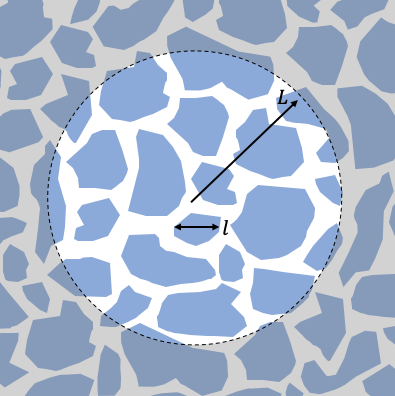
\includegraphics[width=0.4\linewidth]{figs/rev.png}
\caption{Schematic of a \gls{rev} in a multiphase domain. The \gls{rev} has characteristic dimension \(L\), while the pore scale has characteristic dimension \(l\). The blue regions represent the solid phase, while all other regions represent the fluid phase.}
\label{fig:rev}
\end{figure}

Several important notational definitions are needed. Consider a generic field \(\Phi\) in a multi-phase domain. In an approach very similar to the temporal averaging of the Navier-Stokes equations to obtain the \gls{rans} equations, represent \(\Phi\) as the sum of its average \(\la\Phi\ra\) and a fluctuating component \(\hat{\Phi}\) with zero average,

\beq
\label{eq:PM_back}
\Phi=\la\Phi\ra+\hat{\Phi}\ ,
\eeq

\noindent where \(\la\Phi\ra\) is defined as

\beq
\label{eq:AverageDef}
\la\Phi\ra\equiv\frac{1}{\volume}\int_{\volume}\Phi d\volume ,
\eeq

\noindent where \(\volume\) indicates a volume. Eq.\ \eqref{eq:AverageDef} represents the average over all phases. An average over the \(k\) phase is defined as

\beq
\label{eq:AvgDef2}
\la\Phi\ra^k\equiv\frac{1}{\volume_k}\int_{\volume_k}\Phi d\volume\ ,
\eeq

\noindent where \(\volume_k\) is the volume occupied by the \(k\) phase. In order to characterize the distribution of phases in the \gls{rev}, a phase function \(f_k\) is defined as

\beq
\label{eq:PhaseFunction}
f_k=\begin{dcases} 1 & \textrm{in phase $k$}\\ 0 & \textrm{not in phase $k$} \end{dcases}\ .
\eeq

\noindent \(\Phi_k\) represents the value of \(\Phi\) in the \(k\) phase, 

\beq
\label{eq:KPhaseDef}
\Phi_k\equiv\Phi f_k\ ,
\eeq

\noindent while \(\la\Phi_k\ra\) indicates an average of \(\Phi_k\) over all phases,

\beq
\label{eq:PhaseAverage}
\la\Phi_k\ra\equiv\frac{1}{\volume}\int_{\volume}\Phi f_kd\volume\ ,
\eeq

\noindent and \(\la\Phi_k\ra^k\) indicates an average of \(\Phi_k\) over the \(k\) phase,

\beq
\label{eq:IntrinsicPhaseAverage}
\la\Phi_k\ra^k\equiv\frac{1}{\volume_k}\int_{\volume_k}\Phi f_kd\volume\ .
\eeq

\noindent \(\la\Phi_k\ra\) is referred to as the ``extrinsic,'' or ``superficial'' average over phase \(k\), while \(\la\Phi_k\ra^k\) is referred to as the ``intrinsic,'' or ``interstitial'' average over phase \(k\). For fluid flowing in a packed bed, the fluid velocity averaged over the fluid phase represents an intrinsic average. The fluid velocity averaged over both phases, as if the fluid were flowing at the same mass flow rate in an empty bed, represents an extrinsic average. This difference between extrinsic and intrinsic averages plays an important role in the derivation of the porous media equations. 

The porosity \(\epsilon\) for phase \(k\) is the fraction of the total volume occupied by phase \(k\),

\beq
\label{eq:PorosityAvg}
\epsilon_k\equiv\frac{\volume_k}{\volume}\ .
\eeq

\noindent This work considers two-phase fluid-solid domains; an \(f\) subscript refers to the fluid phase and an \(s\) subscript refers to the solid phase. The notational convention used throughout is that \(\epsilon_f\equiv\epsilon\) represents the porosity of the fluid and \(\epsilon_s\equiv1-\epsilon\) represents the porosity of the solid. Models for porosity are described in Section \ref{sec:Porosity}. 

Combining Eqs.\ \eqref{eq:PhaseAverage}--\eqref{eq:PorosityAvg} provides the relationship between intrinsic and extrinsic averages,

\beq
\label{eq:DupuitF}
\la\Phi_k\ra=\epsilon_k\la\Phi_k\ra^k\ .
\eeq

\noindent Applying Eq.\ \eqref{eq:DupuitF} to the extrinsic and intrinsic velocities discussed in the preceding paragraphs,

\beq
\label{eq:DupuitForchiemer}
\vec{v}=\epsilon\vec{V}\ ,
\eeq

\noindent where \(\vec{v}\) is the extrinsic fluid velocity, also referred to as the superficial velocity. \(\vec{V}\) is the intrinsic fluid velocity, also referred to as the interstitial velocity. 

Appendix \ref{sec:PorousMediaMath} provides mathematical identities relating the spatial averages of gradients to the gradients of spatial averages and the spatial averages of time derivatives to the time derivatives of spatial averages. For example, Eq.\ \eqref{eq:TimeAvgDerivativeb} relates the spatial average of a time derivative to the time derivative of a spatial average plus an integral over the phase interface. The key requirement for the use of these identities is that a spatial average be independent of the size of the volume over which it is averaged. Similar restrictions abound in other forms of statistical analysis, such as in requirements of large numbers of coin tosses to accurately estimate the probability of landing tails-up. With the length scales defined in Fig.\ \ref{fig:rev}, this requirement can be expressed as

\beq
\label{eq:LengthReqs}
l\ll L\ .
\eeq

\noindent For packed beds of spherical pebbles, \(l\) is usually taken as either the pebble diameter \(d_p\) or the hydraulic diameter \(D\), which is proportional to \(d_p\). The \gls{rev} scale \(L\) is larger than \(l\) but smaller than the largest bed dimension. The extrinsic and intrinsic averages are functions of space; the average at a location \(\vec{x}\) is interpreted as an average over a \gls{rev} with characteristic dimension \(L\) centered about \(\vec{x}\). A Taylor series analysis performed in Appendix \ref{sec:PorousMediaMath} shows that the assumption that averages are independent of the size of the \gls{rev} is accurate to \(\mathcal{O}(l/L)^2\).

The spatially homogenized conservation equations are now derived using the identities in Appendix \ref{sec:PorousMediaMath}; any notation not explicitly defined here is defined in Appendix \ref{sec:PorousMediaMath}. It is assumed throughout that thermal and pressure gradients are small relative to velocity gradients such that fluctuations in density, thermal conductivity, and isobaric specific heat capacity are much smaller than fluctuations in velocity and can hence be assumed zero \cite{gray}. It is also assumed that the solid-fluid interface is stationary such that \(\vec{V}=\vec{w}\) on the interface and \(\vec{w}=\vec{0}\), where \(\vec{w}\) is the interface velocity. For conciseness, these assumptions are made implicitly while progressing through the derivation, though explicit tracking of these additional terms may be found elsewhere \cite{novak_manual}. The use of each particular identity from Appendix \ref{sec:PorousMediaMath} should be clear from the nature of each kernel, though subtle details will be noted as appropriate.

Spatial averaging of the mass conservation equation in Eq.\ \eqref{eq:ContinuityNonPorous} gives

\beq
\label{eq:PorousMass1}
\frac{\partial\left(\epsilon\la\rho_f\ra^f\right)}{\partial t}+\nabla\cdot\left(\epsilon\la\rho_f\ra^f\la\vec{V}_f\ra^f\right)=0\ ,
\eeq

\noindent where Eq.\ \eqref{eq:DupuitF} was used. For notational simplicity, Eq.\ \eqref{eq:PorousMass1} is rewritten as

\beq
\label{eq:PorousMass}
\frac{\partial(\epsilon\rho_f)}{\partial t}+\nabla\cdot(\epsilon\rho_f\vec{V})=0\ ,
\eeq

\noindent where \(\rho_f\) represents the intrinsic average of fluid density and \(\vec{V}\) represents the intrinsic average of fluid velocity.

%Moving next to the momentum conservation equation in Eq.\ \eqref{eq:NSFullForm}, the time derivative is averaged using Eqs.\ \eqref{eq:TimeAvgDerivativeb} and \eqref{eq:Dispersion}, while the advective, normal stress and deviatoric stress terms are averaged using Eqs.\ \eqref{eq:AvgGrdGrdAvg} and \eqref{eq:Dispersion3}, giving

Spatial averaging of the momentum conservation equation in Eq.\ \eqref{eq:NSFullForm} gives

\beqa
\label{eq:MomFirstStep}
&\frac{\partial(\epsilon\la\rho_f\ra^f\la\vec{V}_f\ra^f)}{\partial t}+\nabla\cdot\left(\epsilon\la\rho_f\ra^f\la\vec{V}_f\ra^f\la\vec{V}_f\ra^f+\la\rho_f\ra^f\la\hat{\vec{V}}_f\hat{\vec{V}}_f\ra\right)=-\epsilon\nabla\la P_f\ra^f+\\
&\hspace{0.5cm}\nabla\cdot\la\tau_f\ra+\frac{1}{\volume}\int_{S_i}\tau_f\hat{n}_fdS-\frac{1}{\volume}\int_{S_i}\left(\hat{P}_f-\la\rho_f\ra^f\hat{\phi}_{g,f}\right)\hat{n}_fdS-\epsilon\la\rho_f\ra^f\nabla\la\phi_{g,f}\ra^f\ .
\eeqa

\noindent The source term \(-\rho_f\nabla\phi_{g,f}\) is related to the gravitational potential \(\phi_{g,f}\) as

\beq
\label{eq:GravitationalPotential}
\nabla\phi_{g,f}\equiv -g\vec{e}_z\ ,
\eeq

%\noindent where averaging was performed using Eqs.\ \eqref{eq:AvgGrdGrdAvgb} and \eqref{eq:Dispersion}, with 

\noindent Terms containing the fluctuation of \(\vec{g}\) are set to zero because the gravitational acceleration vector is constant. 

The advective and deviatoric stress terms were averaged using Eq.\ \eqref{eq:AvgGrdGrdAvga}, but the normal stress term was averaged using Eq.\ \eqref{eq:AvgGrdGrdAvgb}. The different form used for the normal stress is required to correctly enforce that porosity gradients in stagnant fluid systems do not spontaneously induce flows \cite{kececioglu}. For a Newtonian fluid, \(\nabla\cdot\la\tau_f\ra\) becomes

\beqa
\label{eq:DeviatoricStressApprox}
\nabla\cdot\la\tau_f\ra=\nabla\cdot\left\{\la\mu_f\ra\left\lbrack\nabla\la\vec{V}_f\ra+(\nabla\la\vec{V}_f\ra)^T-\frac{2}{3}\nabla\cdot\la\vec{V}_f\ra\textbf{I}\right\rbrack\right\}\ ,
\eeqa

\noindent where the surface integral terms arising from Eq.\ \eqref{eq:AvgGrdGrdAvg} are zero due to the no-slip condition at phase interfaces. The \(\tau_f\hat{n}_f\) integral in Eq.\ \eqref{eq:MomFirstStep} represents the average viscous drag. This term can be expressed in terms of the difference in intrinsic phase velocity difference since the viscous stress is zero if neither phase is moving. Assuming a second-order expansion, the drag term is written as

\beqa
\label{eq:StressApprox}
&\frac{1}{\volume}\int_{S_i}\tau_f\cdot\hat{n}_fdS=\la\mu_f\ra\epsilon\mathscr{A}\left(\la\vec{V}_s\ra^s-\la\vec{V}_f\ra^f\right)+\\
&\hspace{0.5cm}\la\mu_f\ra\epsilon\mathscr{B}:\left(\la\vec{V}_s\ra^s-\la\vec{V}_f\ra^f\right)\cdot\left(\la\vec{V}_s\ra^s-\la\vec{V}_f\ra^f\right)\ ,
\eeqa

\noindent where \(\mathscr{A}\) is a second-order tensor and \(\mathscr{B}\) a third-order tensor. The \(\la\hat{\vec{V}}_f\hat{\vec{V}}_f\ra\) term in Eq.\ \eqref{eq:MomFirstStep} will only be zero if the fluid moves at the same velocity as the fluid-solid interface. This requirement can also be expressed as a two-term expansion,

\beq
\label{eq:MechanicalApprox}
\la\hat{\vec{V}}_f\hat{\vec{V}}_f\ra=\epsilon\mathscr{C}\cdot\left(\la\vec{V}_s\ra^s-\la\vec{V}_f\ra^f\right)+\epsilon\mathscr{L}:\left(\la\vec{V}_s\ra^s-\la\vec{V}_f\ra^f\right)\left(\la\vec{V}_s\ra^s-\la\vec{V}_f\ra^f\right)\ ,
\eeq

\noindent where \(\mathscr{C}\) is a third-order tensor and \(\mathscr{L}\) is a fourth-order tensor. Because \(\la\hat{\vec{V}}_f\hat{\vec{V}}_f\ra\) is symmetric, both of these tensors must be symmetric in their first two indices, and \(\mathscr{L}\) also in the last two indices. 

One more constitutive relationship is required to close the momentum equation. The fluctuating pressure and gravitational field are nonzero perturbations that can still satisfy \(\nabla\la P_f\ra^f+\la\rho_f\ra^f\nabla\la\phi_{g,f}\ra^f=0\), such as when the fluid is hydrostatic. Therefore, expressing this term as a second order expansion gives

\beqa
\label{eq:PressureApprox}
\frac{1}{\volume}\int_{S_i}\left(\hat{P}_f+\la\rho_f\ra^f\hat{\phi}_{g,f}\right)\hat{n}_fdS= \epsilon\mathscr{E}\cdot\left(\nabla\la P_f\ra^f+\la\rho_f\ra^f\nabla\la\phi_{g,f}\ra^f\right)+\hspace{1cm}\\
\epsilon\mathscr{M}:\left(\nabla\la P_f\ra^f+\la\rho_f\ra^f\nabla\la\phi_{g,f}\ra^f\right)\left(\nabla\la P_f\ra^f+\la\rho_f\ra^f\nabla\la\phi_{g,f}\ra^f\right)\ ,
\eeqa

\noindent where \(\mathscr{E}\) is a second-order tensor and \(\mathscr{M}\) is a third-order tensor that is symmetric in its second and third indices. Inserting Eqs.  \eqref{eq:DeviatoricStressApprox}--\eqref{eq:PressureApprox} into Eq.\ \eqref{eq:MomFirstStep} gives the porous media momentum equation for a Newtonian fluid,

\beqa
\label{eq:MomEqnStep2}
\frac{\partial(\epsilon\la\rho_f\ra^f\la\vec{V}_f\ra^f)}{\partial t}+\nabla\cdot\left\lbrack\epsilon\la\rho_f\ra^f\la\vec{V}_f\ra^f\la\vec{V}_f\ra^f+\epsilon\la\rho_f\ra^f\mathscr{C}\cdot\left(\la\vec{V}_s\ra^s-\la\vec{V}_f\ra^f\right)\right\rbrack+\hspace{1.25cm}\\
\nabla\cdot\left\lbrack\epsilon\la\rho_f\ra^f\mathscr{L}:\left(\la\vec{V}_s\ra^s-\la\vec{V}_f\ra^f\right)\left(\la\vec{V}_s\ra^s-\la\vec{V}_f\ra^f\right)\right\rbrack=\hspace{1cm}\\
\nabla\cdot\left\{\la\mu_f\ra\left\lbrack\nabla\la\vec{V}_f\ra+(\nabla\la\vec{V}_f\ra)^T-\frac{2}{3}\nabla\cdot\la\vec{V}_f\ra\textbf{I}\right\rbrack\right\}+\hspace{0.75cm}\\
\la\mu_f\ra\epsilon\mathscr{A}\left(\la\vec{V}_s\ra^s-\la\vec{V}_f\ra^f\right)+\la\mu_f\ra\epsilon\mathscr{B}:\left(\la\vec{V}_s\ra^s-\la\vec{V}_f\ra^f\right)\cdot\left(\la\vec{V}_s\ra^s-\la\vec{V}_f\ra^f\right)-\hspace{0.5cm}\\
\epsilon\left(\textbf{I}+\mathscr{E}\right)\cdot\left(\nabla\la P_f\ra^f+\la\rho_f\ra^f\nabla\la\phi_{g,f}\ra^f\right)-\hspace{0.25cm}\\
\epsilon\mathscr{M}:\left(\nabla\la P_f\ra^f+\la\rho_f\ra^f\nabla\la\phi_{g,f}\ra^f\right)\left(\nabla\la P_f\ra^f+\la\rho_f\ra^f\nabla\la\phi_{g,f}\ra^f\right)\ .
\eeqa

\noindent Models for all of the tensors that appear in Eq.\ \eqref{eq:MomEqnStep2} do not exist. To obtain a tractable momentum equation, mechanical effects of the solid on the fluid are neglected such that \(\mathscr{C}=\textbf{0}\) and \(\mathscr{L}=\textbf{0}\). Second-order effects of the pressure and gravitational forces are also neglected such that \(\mathscr{M}=\textbf{0}\). Both of these approximations are valid for relatively slow flows \cite{gray}. Eq.\ \eqref{eq:MomEqnStep2} then becomes

\beqa
\label{eq:MomEqnStep3a}
\frac{\partial(\epsilon\la\rho_f\ra^f\la\vec{V}_f\ra^f)}{\partial t}+\nabla\cdot\left(\epsilon\la\rho_f\ra^f\la\vec{V}_f\ra^f\la\vec{V}_f\ra^f\right)=-W\la\rho_f\ra^f\la\vec{V}_f\ra^f+\hspace{1cm}\\
\epsilon\nabla\la P_f\ra^f+\nabla\cdot\left(\tilde{\mu}\nabla\langle\vec{V}_f\rangle^f\right)+\epsilon\la\rho_f\ra^f\nabla\la\phi_{g,f}\ra^f\ ,
\eeqa

\noindent where the viscous term in Eq.\ \eqref{eq:MomEqnStep2} has been replaced by a distributed loss friction term that captures the  \(\epsilon\la\mu_f\ra\mathscr{A}(\textbf{I}+\mathscr{E})^{-1}\) and \(\epsilon\la\mu_f\ra\mathscr{B}(\textbf{I}+\mathscr{E})^{-1}\) terms. The sum of these two terms (with \(\mathscr{A}\) divided by \(\la\rho_f\ra^f\) to obtain the proper units) is denoted as \(W\), a combined Darcy and Forchheimer friction factor. A distributed loss friction model is usually sufficient to capture the interphase drag because the length over which the deviatoric stress acts is on the order of several pore diameters \cite{kececioglu}. Models for \(W\) are described in Section \ref{sec:W}.

Some porous media models also include a Brinkman viscous stress term to allow no-slip \glspl{bc} to be applied on boundaries. Brinkman's model expresses the viscous stress term in Eq.\ \eqref{eq:DeviatoricStressApprox} as the sum the Darcy and Forchheimer drag discussed previously plus a velocity laplacian with effective viscosity \(\tilde{\mu}\); such a term is shown in Eq.\ \eqref{eq:MomEqnStep3a} \cite{nield,auwerda_2011,tecdoc1163}. Brinkman's model does not have the same validation basis as either Darcy's or Forchheimer's drag terms, and is generally thought to only be applicable for \(\epsilon>0.8\). At lower porosities, the solid matrix impedes direct transfer of momentum due to viscous forces and the majority of stresses are communicated via pressure \cite{nield}. For completeness, a Brinkman model is included, though the term is usually negligibly small for high Reynolds number reactor applications. Models for \(\tilde{\mu}\) are described in Section \ref{sec:BrinkmanMu}.

For notational simplicity, Eq.\ \eqref{eq:MomEqnStep3a} is written as

\beq
\label{eq:MomEqnStep3}
\frac{\partial(\epsilon\rho_f\vec{V})}{\partial t}+\nabla\cdot(\epsilon\rho_f\vec{V}\vec{V})=-W\rho_f\vec{V}+\epsilon\nabla P+\nabla\cdot(\tilde{\mu}\nabla\vec{V})+\epsilon\rho_f\vec{g}\ ,
\eeq

\noindent where \(\rho_f\) and \(\vec{V}\) have the same interpretation as in Eq.\ \eqref{eq:PorousMass} and \(P\) represents the intrinsic average of pressure.

Only the energy equations remain to be spatially homogenized. Scaling analysis in Section \ref{sec:NonDim} justifies the omission of the viscous heating terms\mdash the \(\nabla\cdot(\vec{V}\tau)\) term in Eq.\ \eqref{eq:EnergyNonPorous} and the \(\tau\colon\nabla\vec{V}\) term in Eq.\ \eqref{eq:InternalEnergy}. Section \ref{sec:NonDim} also justifies neglecting the compression work term proportional to \(dP/dt\). Rather than carry these terms through the derivation for completeness, notational simplicity motivates their omission at the beginning of this derivation. 

Spatial homogenization of the total energy conservation equation in Eq.\ \eqref{eq:EnergyNonPorous} gives

\beqa
\label{eq:Energy1}
&\frac{\partial(\epsilon\la\rho_f\ra^f\la E_f\ra^f)}{\partial t}+\nabla\cdot\left(\epsilon\la\rho_f\ra^f\la H_f\ra^f\la\vec{V}_f\ra^f+\la\rho_f\ra^f\la\hat{H}_f\hat{\vec{V}}_f\ra\right)=\nabla\cdot\left(\la k_f\ra^f\epsilon\nabla\la T_f\ra^f\right)+\\
&\hspace{0.5cm}\nabla\cdot\left( \frac{\la k_f\ra^f}{\volume}\int_{S_i}\hat{T}\hat{n}_fdS\right)+\frac{1}{\volume}\int_{S_i}k_f\nabla T_f\cdot\hat{n}_fdS+\epsilon\la\rho_f\ra^f\la\vec{V}_f\ra^f\cdot\la\vec{g}\ra^f+\la \dot{q}_f\ra\ .
\eeqa

\noindent The surface integral with integrand \(\hat{T}_f\hat{n}_f\) represents the ``tortuosity heat flux.'' The tortuosity heat flux is often very small because convection dominates conduction, and hence is neglected \cite{nakayama}. The surface integral with integrand \(k_f\nabla T_f\cdot\hat{n}_f\) represents the average heat flux at the phase boundary, which is modeled with a convective flux closure as

\beq
\label{eq:ConvecCoolClosure}
\frac{1}{\volume}\int_{S_i}k_f\nabla T_f\hat{n}_fdS=\alpha\left(\la T_s\ra^s-\la T_f\ra^f\right)\ ,
\eeq

\noindent where \(\alpha\) is the convective heat transfer coefficient and \(\la T_s\ra^s\) is the intrinsic phase-averaged solid surface temperature. To obtain the correct units, \(\alpha\) represents the heat transfer coefficient \(h_c\) multiplied by \(a_w\),

\beq
\label{eq:Alpha}
\alpha\equiv a_wh_c\ ,
\eeq

\noindent where \(a_w\) is the wetted area per unit length,

\beq
\label{eq:AwLimit}
a_w=\lim_{\delta\ \to\ 0} \frac{\text{wetted area in domain of length } \delta}{\text{volume of domain of length }\delta}\ .
\eeq

\noindent Models for \(\alpha\) are described in Section \ref{sec:alpha}. Neglecting the tortuosity heat flux and inserting Eq.\ \eqref{eq:ConvecCoolClosure} into Eq.\ \eqref{eq:Energy1}, the total energy conservation equation becomes

\beqa
\label{eq:Energy2}
&\frac{\partial(\epsilon\la\rho_f\ra^f\la E_f\ra^f)}{\partial t}+\nabla\cdot\left(\epsilon\la\rho_f\ra^f\la H_f\ra^f\la\vec{V}_f\ra^f+\la\rho_f\ra^f\la\hat{H}_f\hat{\vec{V}}_f\ra\right)=\\
&\hspace{1cm}\nabla\cdot\left(\la k_f\ra^f\epsilon\nabla\la T_f\ra^f\right)+\epsilon\la\rho_f\ra^f\la\vec{V}_f\ra^f\cdot\la\vec{g}\ra^f+\alpha\left(\la T_s\ra^s-\la T_f\ra^f\right)+\la \dot{q}_f\ra\ .
\eeqa

\noindent Before introducing the final closure for the \(\nabla\cdot(\la\rho_f\ra^f\la\hat{H}_f\hat{\vec{V}}_f\ra)\) term, which will be shared by the spatially homogenized internal energy equation, first homogenize the internal energy equation in Eq.\ \eqref{eq:InternalEnergy}, giving

\beqa
\label{eq:PorousT}
\epsilon\la\rho_f\ra^f\la C_{p,f}\ra^f\frac{\partial\la T_f\ra^f}{\partial t}+\epsilon\la\rho_f\ra^f\la C_{p,f}\ra^f\la\vec{V}_f\ra^f\cdot\nabla\la T_f\ra^f+\la\rho_f\ra^f\la C_{p,f}\ra^f\la\hat{\vec{V}}_f\cdot\hat{\nabla T_f}\ra=\hspace{0.5cm}\\
\nabla\cdot\left(\la k_f\ra^f\epsilon\nabla\la T_f\ra^f\right)+\alpha\left(\la T_s\ra^s-\la T_f\ra^f\right)+\la \dot{q}_f\ra\ ,
\eeqa

\noindent where the spatial homogenization performed for terms shared by the total energy and internal energy equations have been inserted. The tortuosity heat flux term has also been neglected.

Eqs.\ \eqref{eq:Energy2} and \eqref{eq:PorousT} still leave one term that requires closure\mdash the \(\nabla\cdot(\la\rho_f\ra^f\la\hat{H}_f\hat{\vec{V}}_f\ra)\) term in Eq.\ \eqref{eq:Energy2} and the \(\la\rho_f\ra^f\la C_{p,f}\ra^f\la\hat{\vec{V}}_f\cdot\hat{\nabla T_f}\ra\) term in Eq.\ \eqref{eq:PorousT}. These two terms represent enhancements in advective energy transport due to the porous structure, a phenomenon referred to as ``thermal dispersion.'' Thermal dispersion accounts for the effects of changes in flow direction caused by solid obstructions, recirculation flows within the pores, and eddy diffusion in turbulence. Thermal dispersion is represented with a gradient diffusion model,

\beq
\label{eq:ThermalDispersion}
\la\rho_f\ra^f\la C_{p,f}\ra^f\la\hat{\vec{V}}_f\cdot\hat{\nabla T_f}\ra= -\nabla\cdot(\tilde{\kappa}_f\nabla \la T_f\ra^f)\ ,
\eeq

\noindent where \(\tilde{\kappa}_f\) is the thermal dispersion conductivity, which is in general a second-order tensor \cite{nakayama}. While Eq.\ \eqref{eq:ThermalDispersion} is shown in terms of the dispersion kernel in Eq.\ \eqref{eq:PorousT}, a similar interpretation exists for the dispersion kernel in Eq.\ \eqref{eq:Energy2}. 

The effective fluid thermal conductivity \(\kappa_f\) then represents the sum of molecular and dispersion conductivity, 

\beq
\label{eq:KappaFluidDef1}
\kappa_f\equiv\epsilon k_f+\tilde{\kappa}_f\ ,
\eeq

\noindent where the molecular contribution arises from the spatial homogenization of the \(\nabla\cdot(k\nabla T)\) kernel. Models for \(\kappa_f\) are described in Section \ref{sec:Kappa}. Inserting Eqs.\ \eqref{eq:ThermalDispersion} and \eqref{eq:KappaFluidDef1} into Eqs.\ \eqref{eq:Energy2} and \eqref{eq:PorousT} gives

\beqa
\label{eq:Energy3}
&\frac{\partial(\epsilon\la\rho_f\ra^f\la E_f\ra^f)}{\partial t}+\nabla\cdot\left(\epsilon\la\rho_f\ra^f\la H_f\ra^f\la\vec{V}_f\ra^f\right)=\\
&\hspace{1cm}\nabla\cdot\left(\kappa_f\nabla\la T_f\ra^f\right)+\epsilon\la\rho_f\ra^f\la\vec{V}_f\ra^f\cdot\la\vec{g}\ra^f+\alpha\left(\la T_s\ra^s-\la T_f\ra^f\right)+\la \dot{q}_f\ra\ ,
\eeqa

\noindent and

\beqa
\label{eq:PorousT1}
\epsilon\la\rho_f\ra^f\la C_{p,f}\ra^f\frac{\partial\la T_f\ra^f}{\partial t}+\epsilon\la\rho_f\ra^f\la C_{p,f}\ra^f\la\vec{V}_f\ra^f\cdot\nabla\la T_f\ra^f=\hspace{1cm}\\
\nabla\cdot\left(\kappa_f\nabla\la T_f\ra^f\right)+\alpha\left(\la T_s\ra^s-\la T_f\ra^f\right)+\la \dot{q}_f\ra\ .
\eeqa

\noindent For notational simplicity, Eqs.\ \eqref{eq:Energy3} and \eqref{eq:PorousT1} are rewritten as

\beq
\label{eq:EnergyBalance7}
\frac{\partial (\epsilon\rho_f E_f)}{\partial t}+\nabla\cdot(\epsilon H_f\rho_f\vec{V})=\nabla\cdot(\kappa_f\nabla T_f)+\epsilon\rho_f \vec{g}\cdot\vec{V}+\alpha(T_s-T_f)+\dot{q}_f\ ,
\eeq

\noindent and

\beq
\label{eq:EnergyBalanceT}
\epsilon\rho_fC_{p,f}\frac{\partial T_f}{\partial t}+\epsilon\rho_fC_{p,f}\vec{V}\cdot\nabla T_f=\nabla\cdot(\kappa_f\nabla T_f)+\alpha(T_s-T_f)+\dot{q}_f\ ,
\eeq

\noindent where \(\rho_f\) and \(\vec{V}\) have the same interpretation as in Eq.\ \eqref{eq:PorousMass}, \(E_f\) represents the intrinsic average of total energy, \(H_f\) represents the intrinsic average of total enthalpy, \(T_f\) represents the intrinsic average of fluid temperature, \(T_s\) represents the intrinsic average of the solid surface temperature, \(\dot{q}_f\) represents the extrinsic average of the fluid volumetric heat source, and \(C_{p,f}\) represents the intrinsic average of the fluid isobaric specific heat capacity.

The conservation of solid energy equation can be derived by spatially homogenizing the heat equation using the identities in Appendix \ref{sec:PorousMediaMath}. A simpler, but equivalent, approach instead sets \(\vec{V}\) to zero in Eq.\ \eqref{eq:EnergyBalanceT}, replaces all \(f\) subscripts with \(s\) subscripts, and substitutes \(1-\epsilon\) for \(\epsilon\), giving

\beq
\label{eq:SolidPorous}
(1-\epsilon)\rho_sC_{p,s}\frac{\partial T_s}{\partial t}-\nabla\cdot(\kappa_s\nabla T_s)+\alpha(T_s-T_f)-\dot{q}_s=0\ ,
\eeq

\noindent where \(\kappa_s\) represents the effective solid thermal conductivity, \(\rho_s\) represents the intrinsic average of the solid density, \(C_{p,s}\) represents the intrinsic average of the solid isobaric specific heat capacity, and \(\dot{q}_s\) represents the extrinsic average of the solid volumetric heat source. \(\kappa_s\) captures the combined dispersion effects of solid-to-solid radiation \(\kappa_\text{radiation}\), solid-fluid-solid conduction \(\kappa_\text{conduction}\), and solid-to-solid conduction \(\kappa_\text{contact}\),

\beq
\label{eq:Kappa}
\kappa_s\equiv\kappa_{\textrm{radiation}}+\kappa_{\textrm{conduction}}+\kappa_{\textrm{contact}}\ .
\eeq

\noindent Thermal equilibrium is often assumed for geophysical applications, and is even the default in FLUENT's porous media model \cite{fluent}. The inclusion of unique energy conservation equations is essential for modeling of reactor systems due to the volumetric heat sources and the different material properties of the phases \cite{becker,novak_sana}.

In summary, the mass, momentum, and energy conservation equations were spatially homogenized by averaging over a \gls{rev} consisting of a mixture of fluid and solid. Several different models are considered for the macroscale, motivated by the wide range in \gls{th} conditions in \glspl{pbr} and the improved nonlinear convergence behavior that can be obtained by neglecting certain physics kernels. For instance, the inviscid Navier-Stokes model represented by Eqs.\ \eqref{eq:PorousMass}, \eqref{eq:MomEqnStep3} with \(\tilde{\mu}=0\), and \eqref{eq:EnergyBalance7} has two solutions as the Mach number tends to zero\mdash an incompressible limit and an acoustic limit. For nearly incompressible fluids such as molten salts, solution of a compressible model may be an inaccurate representation of the incompressible solution because the incompressible limit is a singular limit of the compressible flow equations \cite{guillard}. A model that neglects the compression work term may provide a better representation of the incompressible solution and enable vastly improved numerical convergence.

Two different models are used depending on the flow conditions and desired level of accuracy\mdash a Navier-Stokes model and a friction-dominated model. The spatially homogenized Navier-Stokes equations on the macroscale are
\begin{subequations}
\label{eq:PorousEquations}
\begin{align}
\label{eq:PMass}\massconservation\ ,\\
\label{eq:PMom}\momentumconservation\ ,\\
\label{eq:PEnergy}\fluidenergyconservation\ ,\\
\label{eq:PSEnergy}\solidenergyconservation\ .
\end{align}
\end{subequations}

\noindent Eq.\ \eqref{eq:PorousEquations} is referred to here as the ``Navier-Stokes model.'' All terms in Eqs.\ \eqref{eq:PMass}--\eqref{eq:PEnergy} have the same form as the local compressible Navier-Stokes equations except the Brinkman stress term, which has the same local form as the incompressible Navier-Stokes viscous stress in order to match literature closures for \(\tilde{\mu}\). An inviscid flow model can be obtained as a simplification of Eq.\ \eqref{eq:PorousEquations} with \(\tilde{\mu}=0\).

For slowly-evolving, low Reynolds number flows, several additional approximations can be made to simplify Eq.\ \eqref{eq:PorousEquations}. Momentum conservation is assumed dominated by friction effects such that changes in pressure are instantaneously reflected as changes in momentum. The total derivative of momentum in Eq.\ \eqref{eq:PMom} is set to zero, giving a pseudo-steady momentum equation. The Brinkman viscosity is also set to zero. Substituting this pseudo-steady momentum equation into the mass conservation in Eq.\ \eqref{eq:PMass} then gives a pressure Poisson equation. Further, compression work is assumed negligible such that energy conservation is well approximated by Eq.\ \eqref{eq:EnergyBalanceT}. Together, these assumptions give,
\begin{subequations}
\label{eq:PrimitiveEqns}
\begin{align}
\label{eq:PMass2}
\legacymass\ ,\\
\label{eq:PMom2}
\legacymomentum\ ,\\
\label{eq:PEnergy2}
\legacyfluidenergy\ ,\\
\label{eq:PSEnergy2}
\legacysolidenergy\ .
\end{align}
\end{subequations}

\noindent Eq.\ \eqref{eq:PrimitiveEqns} is referred to here as the ``friction-dominated model.'' This friction-dominated model has been widely used for the analysis of \glspl{pbr} \cite{hossain, nouri, tecdoc1163}.  

Pebbles move continuously through the bed in online refueling operation. Depending on the design, pebbles cycle between 2 and 10 times over a period of several years. The velocity of these motions is orders of magnitude smaller than the fluid velocity. The kinetic energies of pebbles in fluidized beds such as liquid salt systems are also negligibly small \cite{mardus_hall}. Therefore, porosity is assumed independent of time such that it is moved outside the time derivatives in Eqs.\ \eqref{eq:PorousEquations} and \eqref{eq:PrimitiveEqns}.

As will be discussed at greater length in Chapter \ref{sec:ph}, Eqs.\ \eqref{eq:PorousEquations} and \eqref{eq:PrimitiveEqns} may be solved for a number of different solution variables to enable general simulation of compressible and incompressible flows, flexible application of the \glspl{bc} described in Section \ref{sec:BCs}, and better numerical convergence in the presence of certain material discontinuities \cite{hauke_1998}. These solution variables are the primitive interstitial set \(P\), \(\vec{V}\), and \(T_f\); the primitive superficial set \(P\), \(\vec{v}\), and \(T_f\); the mixed interstitial set \(P\), \(\rho_f\vec{V}\), and \(T_f\); the mixed superficial set \(P\), \(\rho_f\vec{v}\), and \(T_f\); and the conservative interstitial set \(\rho_f\), \(\rho_f\vec{V}\), and \(\rho_fE_f\).

\subsection{Non-Dimensional Analysis}
\label{sec:NonDim}

This section presents a brief scaling analysis of the momentum and energy conservation equations to justify omission of the viscous heating term from Eqs.\ \eqref{eq:PorousEquations} and \eqref{eq:PrimitiveEqns} and the compression work term from Eq.\ \eqref{eq:PrimitiveEqns}. For notational simplicity, this scaling analysis is performed starting from the local conservation equations because small terms were neglected at the outset of the spatial homogenization procedure, rather than carried through to be neglected at the conclusion.

Scaling analysis begins with the \gls{1d} form of momentum conservation in Eq.\ \eqref{eq:NSFullForm}. Define the following nondimensional quantities,

\beq
\label{eq:NondimensionalQuantities}
t^+=\frac{t}{L/V_o},\quad V^+=\frac{V}{V_o},\quad P^+=\frac{P}{\rho_oV_o^2},\quad x^+=\frac{x}{L},\quad g^+=\frac{g}{g_o}\ ,
\eeq

\noindent where a \(+\) superscript indicates a nondimensional quantity. Inserting Eq.\ \eqref{eq:NondimensionalQuantities} into the \gls{1d} form of Eq.\ \eqref{eq:NSFullForm} with constant viscosity and dividing through by the coefficient on the advective term gives

\beqa
\label{eq:NondimensionalNS2}
\frac{dV^+}{dx^+}=&\ \frac{Lg_o}{V_o^2}g^+-\frac{\partial P^+}{\partial x^+}+\frac{1}{Re}\frac{\partial}{\partial {x^+}}\left(\diamond\right)\ ,
\eeqa

\noindent where the viscous term is represented symbolically as \(\diamond\) and \(Re\) is the Reynolds number. For a generic porous medium characterized by two different velocity scales \(v\) and \(V\) and two different length scales \(d_p\) and \(D\), there are many manners in which the Reynolds number can be defined. The two most common definitions are
\begin{subequations}
\label{eq:RePorousGeneral}
\begin{align}
\label{eq:RePorousGeneralA}
Re=&\ \frac{\rho \|\vec{v}\|d_p}{\mu}\ ,\\
\label{eq:RePorousGeneralB}
Re_h=&\ \frac{\rho \|\vec{V}\|D}{\mu}\ .
\end{align}
\end{subequations}

\noindent Both Eqs.\ \eqref{eq:RePorousGeneralA} and \eqref{eq:RePorousGeneralB} are used throughout this work depending on whether the domain in question is porous or open, respectively. 

Non-dimensionalization of the energy conservation equation is performed beginning from the \gls{1d} form of Eq.\ \eqref{eq:InternalEnergy} with the volumetric heat source omitted for simplicity. In addition to Eq.\ \eqref{eq:NondimensionalQuantities}, define

\beq
\label{eq:Nondim11}
T^+=\frac{T}{\Delta T}\ .
\eeq

\noindent Inserting Eqs.\ \eqref{eq:NondimensionalQuantities} and \eqref{eq:Nondim11} into the \gls{1d} form of Eq.\ \eqref{eq:InternalEnergy} with constant thermal conductivity and dividing through by the coefficient on the advective term gives

\beq
\label{eq:NondimensionalTemperatureEqn}
\frac{dT^+}{dt^+}-\beta Ec\ T^+\frac{dP^+}{dt^+}=\frac{Br}{Pe}(\diamond)-\frac{1}{Pe}\frac{\partial}{\partial x^+}\frac{\partial T^+}{\partial x^+}\ ,
\eeq

\noindent where the viscous power term is represented symbolically as \(\diamond\). \(Pe\) is the Peclet number, defined as

\beq
\label{eq:PecletDef}
Pe\equiv\frac{\rho C_{p}\|\vec{V}\|L}{k}\ ;
\eeq

%High-Prandtl number fluids, such as molten salts, at Reynolds number typical of reactor operation display greater heat transfer caused by turbulence than diffusion \cite{song}. 

\noindent\(Ec\) is the Eckert number, defined as

\beq
\label{eq:EcNumber}
Ec=\frac{\|\vec{V}\|^2}{C_{p}\Delta T}\ ;
\eeq

\noindent and \(Br\) is the Brinkman number, defined as

\beq
\label{eq:BrNumber}
Br=\frac{\mu \|\vec{V}\|^2}{k\Delta T}\ .
\eeq

\noindent Viscous heating is negligible if \(Br/Pe\ll1\) and compression work is negligible if \(\beta Ec\ll1\). Table \ref{table:TypicalData} provides estimates of these dimensionless numbers for five representative reactor designs\mdash the sodium-cooled \gls{pfbr}, the helium-cooled \gls{thtr}, the \gls{flibe}-cooled \gls{pbfhr}, the water-cooled \gls{ap1000}, and the CO$_2$-cooled \gls{agr}. 

\begin{table}[!h]
\caption{Approximate operating conditions and nondimensional numbers for representative nuclear reactor designs \cite{pfbr,pfbrTH,thtr_1990,pbfhr,ap1000,ap1000_2,nonbol}. Temperatures are listed as ``inlet/outlet.''}
\centering
\begin{tabular}{@{}l l l l l l@{}}
\toprule
\textbf{Parameter} & \textbf{PFBR} & \textbf{THTR} & \textbf{PB-FHR} & \textbf{AP-1000} & \textbf{AGR}\\
\midrule
Coolant							& sodium			& helium				& \gls{flibe}				& water				& CO\textsubscript{2}\\
Power (MWth)				& 1250			& 750				& 236				& 3400				& 1623\\
Fuel	 geometry							& assembly		& pebble				& pebble				& assembly			& assembly\\
Pressure (\si{\mega\pascal})						& 0.1				& 4.0					& 0.1					& 15.5				& 4.1\\
Temperature (\si{\celsius})				& 400/550		& 250/750				& 600/700				& 280/325				& 340/640\\
Flowrate (\si{\kilo\gram\per\second})						& 6390			& 298				& 976				& 13700				& 4060\\
Velocity (\si{\meter\per\second})						& 4.8				& 12.0				& 0.4					& 4.8				& 1.6\\
 \(D\) (mm)						& 5.0				& 26.0				& 13.0				& 11.7			& 38.0\\
 \(\rho\) (\si{\kilo\gram\per\cubic\meter})			& 840			& 2.5					& 2000				& 720			& 28\\
 \(\mu\) (\(10^{-5}\) Pa\(\cdot\)s)			& 25				& 3.9					& 680				& 8.7				& 3.4\\
 \(k\) (\si{\watt\per\meter\per\kelvin})					& 139			& 0.30				& 1.10				& 0.56			& 0.05\\
 \(C_p\) (\si{\joule\per\kilo\gram\per\kelvin})				& 1268			& 5195				& 2416				& 5534			& 1157\\
 \(Pr\)							& 0.002			& 0.67				& 15.0				& 0.86			& 0.79\\
 \(Br\)							& \(2.7\times10^{-7}\)& \(3.7\times10^{-5}\)	& \(9.9\times10^{-6}\)	& \(7.8\times10^{-5}\)	& \(5.8\times10^{-6}\)\\
 \(Re\)							& \(8.2\times10^{+4}\)	& \(2.0\times10^{+4}\)		& \(1.5\times10^{+3}\)		& \(4.6\times10^{+5}\)		& \(5.0\times10^{+4}\)\\
 \(Pe\)							& \(1.8\times10^{+2}\)	& \(1.3\times10^{+4}\)		& \(2.3\times10^{+4}\)		& \(4.0\times10^{+5}\)		& \(4.0\times10^{+4}\)\\
 \(Ec\) & \(1.2\times10^{-4}\) & \(5.5\times10^{-5}\) & \(6.6\times10^{-7}\) & \(9.0\times10^{-5}\) & \(7.4\times10^{-6}\)\\
 \(Br/Pe\)							& \(1.5\times10^{-9}\)& \(2.8\times10^{-9}\)	& \(4.3\times10^{-10}\)	& \(2.0\times10^{-10}\)	& \(1.5\times10^{-10}\)\\
 \(\Delta T/T\) & \(2.2\times10^{-1}\) & \(9.6\times10^{-1}\) & \(1.1\times10^{-1}\) & \(8.3\times10^{-2}\) & \(4.9\times10^{-1}\)\\
\bottomrule
\end{tabular}
\label{table:TypicalData}
\end{table}

For all five designs, both viscous heating and compression work are orders of magnitude less significant than energy advection and can therefore be neglected from the macroscale model. But while \(Re\gg1\) for most applications, the Brinkman viscous stress is retained in the macroscale model for completeness and application of no-slip \glspl{bc}. Likewise, \(Pe\gg1\) for all systems considered, but thermal energy conduction is retained in the macroscale model because the gradient diffusion model for thermal dispersion always requires a diffusive kernel.

\subsection{Boundary and Initial Conditions}
\label{sec:BCs}

This section describes the \glspl{bc} and \glspl{ic} for the macroscale conservation equations. Because of the presence of advective and diffusive terms, the fluid conservation equations are a mixed hyperbolic-parabolic system. Lacking advective terms, the solid energy conservation equation is a parabolic equation. For systems of equations that permit real wave propagation, which include hyperbolic and parabolic equations, a well-posed set of \glspl{bc} and \glspl{ic} requires consideration of the direction of information propagation. Conditions may only be imposed on boundaries where the eigenvalues of the homogeneous portion of the equations are positive relative to the unit normal of the boundary\mdash  in other words, where characteristics enter the domain \cite{hirsch}. For both the fluid and solid conservation equations, \glspl{ic} are required for all variables throughout the entire domain at \(t=0\). The remainder of this section describes the \glspl{bc} for the conservation equations.

\subsubsection{The Fluid Conservation Equations}

Despite the mixed hyperbolic-parabolic character of the fluid conservation equations, advection dominates diffusion at reactor conditions such that well-posed \glspl{bc} can be based on well-posed conditions for purely hyperbolic systems. The hyperbolic versions of the fluid conservation equations are obtained by omitting all diffusive kernels from Eqs.\ \eqref{eq:PorousEquations} and \eqref{eq:PrimitiveEqns}. Such a hyperbolic equation in \(n_{sd}\) spatial dimensions has eigenvalues \(-\vec{V}\cdot\hat{n}-c\), \(-\vec{V}\cdot\hat{n}+c\), and \(-\vec{V}\cdot\hat{n}\), where \(c\) is the speed of sound, \(\hat{n}\) is the boundary unit outward normal, and the \(\vec{V}\cdot\hat{n}\) eigenvalue occurs once for each spatial dimension \cite{rohde}. 

All flows are assumed subsonic such that \(\|\vec{V}\|<c\). On inlet and no-penetration boundaries, \(n_{sd}+1\) eigenvalues are positive and one eigenvalue is negative, which requires imposition of \(n_{sd}+1\) conditions. On outlet boundaries, one eigenvalue is positive and \(n_{sd}+1\) eigenvalues are negative, which requires imposition of one condition.

The \gls{fe} discretization described in Section \ref{sec:fem} converts the strong forms in Eqs.\ \eqref{eq:PorousEquations} and \eqref{eq:PrimitiveEqns} to weak forms that contain both volume and surface integrals. The surface integrals represent flux \glspl{bc} that must be specified regardless of the type of boundary\mdash inflow, outflow, or no-penetration\mdash unless a Dirichlet \gls{bc} already strongly enforces a condition on that boundary. For example, the Navier-Stokes mass conservation equation weak form in Eq.\ \eqref{eq:MassWeak} contains the following surface integral,

\beq
\label{eq:q1}
\int_{\Gamma}\epsilon\rho_f\vec{V}\cdot\hat{n}d\Gamma\ ,
\eeq

\noindent where \(\Gamma\) is the boundary with unit outward normal \(\hat{n}\). On boundaries where an interstitial mass flowrate \(\dot{m}\) is specified, the above integral is evaluated as

\beq
\int_{\Gamma}\epsilon\dot{m}d\Gamma\ .
\eeq

\noindent On boundaries where a mass flowrate is not specified and no Dirichlet condition is applied, the weak form still contains the surface integral in Eq.\ \eqref{eq:q1}, which must be evaluated using the implicit solution values for \(\rho_f\) and \(\vec{V}\). This is referred to here as an ``implicit'' \gls{bc}. 

This distinction between imposed and implicit \glspl{bc} is important for understanding the \gls{bc} requirements for the macroscale model. On each boundary, a Dirichlet or Neumann condition must be applied to each conservation equation simply due to the nature of the boundary integrals in the \gls{fe} weak form\hspace{0.02cm}\footnote{While ``Neumann'' conditions strictly refer to \glspl{bc} where the derivative is enforced, here the looser convention of referring to all integrated \glspl{bc} as ``Neumann'' is followed.}. In \(n_{sd}\) spatial dimensions, this results in \(n_{sd}+2\) conditions on each boundary. The eigenvalue analysis then provides information on what subset of these conditions must be imposed by the modeler, rather than implicit. The eigenvalue analysis for inlet and no-penetration boundaries shows the \(n_{sd}+1\) conditions corresponding to positive eigenvalues must be of Dirichlet or specified Neumann type, while the remaining condition corresponding to the negative eigenvalue must be of implicit Neumann type. On outlet boundaries, one condition must be of Dirichlet or specified Neumann type, while the remaining \(n_{sd}+1\) conditions must be of implicit Neumann type. 

The remainder of this section describes Dirichlet and Neumann \glspl{bc} for the fluid conservation equations subject to these constraints. Neumann \glspl{bc} are additive within the numerical implementation, so are discussed individually. On inlet boundaries, temperature and either velocity or momentum are specified. Velocity and momentum may be specified in either an interstitial or superficial basis. On outlet boundaries, pressure is specified. On solid walls and \(r\)-\(z\) symmetry boundaries, mass conservation requires the no-penetration condition. On solid walls, the tangential velocity component may optionally be set to zero with what is referred to as a ``no-slip'' condition. On solid boundaries, the solid temperature or heat flux may be specified. 

The boundary is the union of the inlet \(\Gamma_\text{in}\), outlet \(\Gamma_\text{out}\), wall \(\Gamma_\text{wall}\), and $r$-$z$ symmetry axis \(\Gamma_\text{$r$-$z$ symmetry}\),

\beq
\label{eq:q8}
\Gamma\equiv\Gamma_\text{in}\cup\Gamma_\text{out}\cup\Gamma_\text{wall}\cup\Gamma_\text{$r$-$z$ symmetry}\ ,
\eeq

\noindent where the intersection of the \(j\)-th term on the \gls{rhs} of Eq.\ \eqref{eq:q8} with the \(k\)-th term on the \gls{rhs} of Eq.\ \eqref{eq:q8} is the empty set for \(j\neq k\). The inlet boundary is the union of boundaries on which the interstitial velocity, superficial velocity, interstitial momentum, and superficial momentum are specified,

\beqa
\label{eq:q7}
\Gamma_\text{in}\equiv\Gamma_\text{in, interstitial velocity}\cup\Gamma_\text{in, superficial velocity}\ \cup\hspace{1cm}\\
\Gamma_\text{in, interstitial momentum}\cup\Gamma_\text{in, superficial momentum}\ ,
\eeqa

\noindent where the intersection of the \(j\)-th term on the \gls{rhs} of Eq.\ \eqref{eq:q7} with the \(k\)-th term on the \gls{rhs} of Eq.\ \eqref{eq:q7} is the empty set for \(j\neq k\). The wall boundary is the union of the slip and no-slip boundaries, 

\beq
\Gamma_\text{wall}\equiv\Gamma_\text{wall, slip}\cup\Gamma_\text{wall, no-slip}\ ,
\eeq

\noindent where \(\Gamma_\text{wall, slip}\cap\Gamma_\text{wall, no-slip}=\emptyset\). The wall boundary is also the union of the specified temperature and heat flux boundaries,

\beq
\Gamma_\text{wall}\equiv\Gamma_\text{wall, temperature}\cup\Gamma_\text{wall, heat flux}\ ,
\eeq

\noindent where \(\Gamma_\text{wall, temperature}\cap\Gamma_\text{wall, heat flux}=\emptyset\). The heat flux boundary is understood to consist of a variety of different representations of heat flux, such as conduction, convection, and radiation, which may have a nonzero intersection with one another. 

Finally, an \(i\) subscript refers to an ``imposed,'' or specified, value, while any term lacking a subscript refers to the implicit solution value. Functional notation, such as \(\rho_f(P,T_f)\), indicates the use of the \gls{eos} to obtain \(\rho_f\) from \(P\) and \(T_f\). 

For the mass conservation equation in Eqs.\ \eqref{eq:PMass} and \eqref{eq:PMass2}, the outlet condition for pressure as the nonlinear variable is

\beq
\label{eq:MassOut1}
P=P_i\text{ for }\Gamma\in\Gamma_\text{out}\ ,
\eeq

\noindent while the outlet condition for density as the nonlinear variable is a fully-implicit condition with pressure weakly imposed in the momentum \glspl{bc},

\beq
\label{eq:MassOut2}
\epsilon\rho_f\vec{V}\cdot\hat{n}=\epsilon\rho_f\vec{V}\cdot\hat{n}\text{ for }\Gamma\in\Gamma_\text{out}\ .
\eeq

\noindent The Neumann-type \glspl{bc} for the advective flux integral for the remaining boundaries are

\beq
\epsilon\rho_f\vec{V}\cdot\hat{n}=
\begin{dcases}
0 & \Gamma\in\Gamma_\text{wall}\\
0 & \Gamma\in\Gamma_\text{$r$-$z$ symmetry}\\
\epsilon\rho_f\vec{V}_i\cdot\hat{n} & \Gamma\in\Gamma_\text{in, interstitial velocity}\\
\rho_f\vec{v}_i\cdot\hat{n} & \Gamma\in\Gamma_\text{in, superficial velocity}\\
\epsilon(\rho_f\vec{V})_i\cdot\hat{n} & \Gamma\in\Gamma_\text{in, interstitial momentum}\\
(\rho_f\vec{v})_i\cdot\hat{n} & \Gamma\in\Gamma_\text{in, superficial momentum}\\
\end{dcases}\ .
\eeq

\noindent For the momentum conservation equation in Eqs.\ \eqref{eq:PMom} and \eqref{eq:PMom2}, a Dirichlet value of velocity or momentum is specified on the inlet. If the nonlinear variable is interstitial velocity, the inlet \gls{bc} is

\beq
\label{eq:q6}
\vec{V}=
\begin{dcases}
\vec{V}_i & \Gamma\in\Gamma_\text{in, interstitial velocity}\\
\vec{v}_i/\epsilon & \Gamma\in\Gamma_\text{in, superficial velocity}\\
(\rho_f\vec{V})_i/\rho_f(P,T_{f,i}) & \Gamma\in\Gamma_\text{in, interstitial momentum}\\
(\rho_f\vec{v})_i/\left\lbrack\epsilon\rho_f(P,T_{f,i})\right\rbrack & \Gamma\in\Gamma_\text{in, superficial momentum}\\
\end{dcases}\ .
\eeq

\noindent If the nonlinear variable is superficial velocity, the inlet \gls{bc} is

\beq
\vec{v}=
\begin{dcases}
\epsilon\vec{V}_i & \Gamma\in\Gamma_\text{in, interstitial velocity}\\
\vec{v}_i & \Gamma\in\Gamma_\text{in, superficial velocity}\\
\epsilon(\rho_f\vec{V})_i/\rho_f(P,T_{f,i}) & \Gamma\in\Gamma_\text{in, interstitial momentum}\\
(\rho_f\vec{v})_i/\rho_f(P,T_{f,i}) & \Gamma\in\Gamma_\text{in, superficial momentum}\\
\end{dcases}\ .
\eeq

\noindent If the nonlinear variable is interstitial momentum, the inlet \gls{bc} is

\beq
\rho_f\vec{V}=
\begin{dcases}
\rho_f(P,T_{f,i})\vec{V}_i & \Gamma\in\Gamma_\text{in, interstitial velocity}\\
\rho_f(P,T_{f,i})\vec{v}_i/\epsilon & \Gamma\in\Gamma_\text{in, superficial velocity}\\
(\rho_f\vec{V})_i & \Gamma\in\Gamma_\text{in, interstitial momentum}\\
(\rho_f\vec{v})_i/\epsilon & \Gamma\in\Gamma_\text{in, superficial momentum}\\
\end{dcases}\ .
\eeq

\noindent If the nonlinear variable is superficial momentum, the inlet \gls{bc} is

\beq
\label{eq:q7}
\rho_f\vec{v}=
\begin{dcases}
\epsilon\rho_f(P,T_{f,i})\vec{V}_i & \Gamma\in\Gamma_\text{in, interstitial velocity}\\
\rho_f(P,T_{f,i})\vec{v}_i & \Gamma\in\Gamma_\text{in, superficial velocity}\\
\epsilon(\rho_f\vec{V})_i & \Gamma\in\Gamma_\text{in, interstitial momentum}\\
(\rho_f\vec{v})_i & \Gamma\in\Gamma_\text{in, superficial momentum}\\
\end{dcases}\ .
\eeq

\noindent For no-slip solid walls, additional Dirichlet-type \glspl{bc} are one of
\begin{subequations}
\begin{align}
\vec{V}=&\ \vec{0}\text{ for }\Gamma\in\Gamma_\text{wall, no-slip}\ ,\\
\vec{v}=&\ \vec{0}\text{ for }\Gamma\in\Gamma_\text{wall, no-slip}\ ,\\
\rho_f\vec{V}=&\ \vec{0}\text{ for }\Gamma\in\Gamma_\text{wall, no-slip}\ ,\\
\rho_f\vec{v}=&\ \vec{0}\text{ for }\Gamma\in\Gamma_\text{wall, no-slip}\ ,
\end{align}
\end{subequations}

\noindent depending on the nonlinear solution variable. The Neumann-type \glspl{bc} for the advective flux integral in the \(j\)-th momentum equation for the remaining boundaries are

\beq
\epsilon\rho_fV_j\vec{V}\cdot\hat{n}=
\begin{dcases}
0 & \Gamma\in\Gamma_\text{wall, slip}\\
0 & \Gamma\in\Gamma_\text{$r$-$z$ symmetry}\\
\epsilon\rho_fV_j\vec{V}\cdot\hat{n}  & \Gamma\in\Gamma_\text{out}\\
\end{dcases}\ .
\eeq

\noindent The Neumann-type \glspl{bc} for the pressure integral in the \(j\)-th momentum equation for the remaining boundaries are

\beq
\epsilon Pn_j=
\begin{dcases}
\epsilon Pn_j & \Gamma\in\Gamma_\text{wall, slip}\\
\epsilon Pn_j & \Gamma\in\Gamma_\text{$r$-$z$ symmetry}\\
\epsilon P_in_j & \Gamma\in\Gamma_\text{out}
\end{dcases}\ .
\eeq

\noindent The Neumann-type \glspl{bc} for the diffusive flux integral in the \(j\)-th momentum equation for the remaining boundaries are

% TODO: confirm that this is correct for the slip case
\beq
-\tilde{\mu}\nabla V_j\cdot\hat{n}=
\begin{dcases}
-\tilde{\mu}\nabla V_j\cdot\hat{n} & \Gamma\in\Gamma_\text{wall, slip}\\
0 & \Gamma\in\Gamma_\text{$r$-$z$ symmetry}\\
-\tilde{\mu}\nabla V_j\cdot\hat{n} & \Gamma\in\Gamma_\text{out}
\end{dcases}\ .
\eeq

\noindent For the energy conservation equation in Eqs.\ \eqref{eq:PEnergy} and \eqref{eq:PEnergy2}, a Dirichlet value of temperature is specified on the inlet and on walls where temperature is specified. If the nonlinear variable is temperature, this \gls{bc} is

\beq
T_f=T_{f,i}\text{ for }\Gamma\in\Gamma_\text{in}\cup\Gamma_\text{wall, temperature}\ ,
\eeq

\noindent while if the nonlinear variable is total fluid energy, this \gls{bc} is

\beq
\label{eq:q5}
\rho_fE_f=\rho_f(P,T_{f,i})\left\lbrack e_f(P,T_{f,i})+\frac{1}{2}\vec{V}\cdot\vec{V}\right\rbrack\text{ for }\Gamma\in\Gamma_\text{in}\cup\Gamma_\text{wall, temperature}\ .
\eeq

\noindent For brevity, Eq.\ \eqref{eq:q5} is written in terms of the implicit values of velocity at the inlet rather than the many combinations of specified velocity and momentum as represented by Eqs.\ \eqref{eq:q6}--\eqref{eq:q7}. Because Dirichlet \glspl{bc} are strongly imposed within the \gls{fe} discretization, no approximation is made in this notational simplification. 

No advective flux integral appears in the weak form of Eq.\ \eqref{eq:PEnergy2}. The Neumann-type \glspl{bc} for the advective flux integral in Eq.\ \eqref{eq:PEnergy} for the remaining boundaries are

\beq
\epsilon\rho_fH_f\vec{V}\cdot\hat{n}=
\begin{dcases}
0 & \Gamma\in\Gamma_\text{wall}\\
0 & \Gamma\in\Gamma_\text{$r$-$z$ symmetry}\\
\epsilon\left\{\rho_f\left\lbrack e_f(P_i,T_f)+\frac{1}{2}\vec{V}\cdot\vec{V}\right\rbrack+P_i\right\}\vec{V}\cdot\hat{n} & \Gamma\in\Gamma_\text{out}
\end{dcases}\ .
\eeq

\noindent The Neumann-type \glspl{bc} for the diffusive flux integral for the remaining boundaries are

\beq
\label{eq:fluid_bcs}
-\kappa_f\nabla T_f\cdot\hat{n}=
\begin{dcases}
\tilde{q} & \Gamma\in\Gamma_\text{wall, heat flux (generic)}\\
-k_\infty\nabla T_\infty\cdot\hat{n} & \Gamma\in\Gamma_\text{wall, heat flux (conduction)}\\
h_c(T_f-T_\infty) & \Gamma\in\Gamma_\text{wall, heat flux (convection)}\\
\varepsilon\sigma(T_f^4-T_\infty^4) & \Gamma\in\Gamma_\text{wall, heat flux (radiation)}\\
0 & \Gamma\in\Gamma_\text{$r$-$z$ symmetry}\\
-\kappa_f\nabla T_f\cdot\hat{n} & \Gamma\in\Gamma_\text{out}
\end{dcases}\ ,
\eeq

\noindent where \(\tilde{q}\) represents a generic heat flux, the \(\infty\) subscripts refer to the domain adjacent to the boundary, \(h_c\) is the convective heat transfer coefficient, \(\varepsilon\) is the surface emissivity, and \(\sigma\) is the Boltzmann constant.

\subsubsection{The Solid Energy Conservation Equation}

The parabolic character of the solid energy conservation equation permits \glspl{bc} to be applied on any boundary of the domain; these boundaries are either temperature, heat flux, or $r$-$z$ symmetry boundaries, irrespective of whether the boundary represents a fluid inlet, outlet, or wall,

\beq
\label{eq:q9}
\Gamma\equiv\Gamma_\text{temperature}\cup\Gamma_\text{heat flux}\cup\Gamma_\text{$r$-$z$ symmetry}\ ,
\eeq

\noindent where the intersection of the \(j\)-th term on the \gls{rhs} of Eq.\ \eqref{eq:q9} with the \(k\)-th term on the \gls{rhs} of Eq.\ \eqref{eq:q9} is the empty set for \(j\neq k\). A Dirichlet temperature is specified as

\beq
T_s=T_{s,i}\text{ for }\Gamma\in\Gamma_\text{temperature}\ .
\eeq

\noindent The Neumann-type \glspl{bc} for the diffusive flux integral for the remaining boundaries are

\beq
\label{eq:solid_bcs}
-\kappa_s\nabla T_s\cdot\hat{n}=
\begin{dcases}
\tilde{q} & \Gamma\in\Gamma_\text{heat flux (generic)}\\
-k_\infty\nabla T_\infty\cdot\hat{n} & \Gamma\in\Gamma_\text{heat flux (conduction)}\\
h_c(T_s-T_\infty) & \Gamma\in\Gamma_\text{heat flux (convection)}\\
\varepsilon\sigma(T_s^4-T_\infty^4) & \Gamma\in\Gamma_\text{heat flux (radiation)}\\
0 & \Gamma\in\Gamma_\text{$r$-$z$ symmetry}\\
\end{dcases}\ .
\eeq

\subsection{Closures}
\label{sec:Closures}

This section describes models used for the macroscale closures\mdash the porosity, \(\epsilon\); the interphase friction factor, \(W\); the Brinkman viscosity, \(\tilde{\mu}\); the interphase convective heat transfer coefficient, \(\alpha\); the effective fluid thermal conductivity, \(\kappa_f\); and the effective solid thermal conductivity, \(\kappa_s\). Each discussion coincides with a description of the salient physical phenomena represented by that closure to provide context and background necessary to understand modeling choices made in later chapters. In addition, the intrinsic phase-averaged fluid properties \(\rho_f\), \(C_{p,f}\), \(k_f\), and \(\mu_f\) are described in Section \ref{sec:FPs}. A description of the intrinsic phase-averaged solid properties \(\rho_s\), \(C_{p,s}\), and \(k_s\) is deferred until Section \ref{sec:meso_props} to collocate the discussion with property models used for the meso length scales.

The macroscale porous media model derived in Section \ref{sec:macro_deriv} is applicable to a wide range of physical systems. However, unless otherwise noted, all closures described Sections \ref{sec:Porosity}--\ref{sec:KappaS} apply to random packed beds comprised of uniform diameter spherical pebbles.

\subsubsection{Porosity}
\label{sec:Porosity}

The porosity represents the fluid volume fraction in each \gls{rev} and has an important impact on flow and heat transfer\mdash all other closures described in Sections \ref{sec:W}--\ref{sec:KappaS} are generally dependent on porosity. Porosity also impacts the local flow area and appears in most kernels in the macroscale conservation equations. Lower porosities result in more tortuous fluid paths, and consequentially frictional momentum losses and greater convective heat transfer. Depending on the relative thermal conductivities of the phases, the conduction components of the effective solid thermal conductivity may increase or decrease with porosity, while the larger void spaces associated with higher porosities increase the effective radiation heat transfer component \cite{you}. 

The random packing of beds is often numerically modeled with the \gls{dem}, where Newton's laws of motion are solved for a collection of granular pebbles considering friction, contact plasticity, gravity, and a variety of potentials \cite{duToit2008,auwerda2013,rycroft,abdalla,suikkanen,y_li,auwerda_2011,zhang2016}. Alternatively, experimentalists may fill a container with spheres, pour in a wax or resin that is allowed to solidify, and then chop the container into pieces for weighing after melting of the wax or resin \cite{goodling,benenati,roblee}. Other techniques such as image analysis, photography, radiography, and centripetal acceleration have been used \cite{goodling1985,mueller,giese}. A mesh is then superimposed on this data, and the porosity in each cell of the mesh evaluated as a volume average over that cell plus a number of that cell's neighboring cells. This spatial dependence may then be directly used in a physics application or correlated with a functional fit. 

The present analysis only considers existing literature models for cylindrical beds, which tend to closely resemble many \gls{pbr} core geometries. These models assume smooth walls and beds without alignment structures such as control rods or guiding plates \cite{bai,rycroft} and that porosity is flow- and time-independent \cite{y_li,li}. The spherical pebbles are also assumed to be larger than 0.1 \si{\milli\meter} in diameter such that Van der Waals forces, or the distance-dependent forces between atoms, are insignificant \cite{yang2000}.

The porosity is a function of the distance from walls and free surfaces. In the radial direction, the porosity is a damped, oscillatory function of the distance from the bounding walls, reaching a nearly constant value four to five pebble diameters from the wall \cite{auwerda2013,benenati,cohen,klerk,duToit2008,giese,goodling,roblee,mueller}. The porosity at the wall is unity due to sphere alignment and attains a global minimum at about \(d_p/2\) distance normal from the wall. The high porosity near the walls results in lower drag and a flow-channeling effect, with a peak in the velocity near the wall that is usually 1.5 to 10 times larger than the bulk velocity \cite{vortmeyer,amiri,y_li,amini,martin,lerou,white,cohen,giese,zhang2016}. This bypass flow results in less effective bulk bed cooling, higher bed temperatures \cite{auwerda_2011,becker}, more nonuniform outlet temperatures \cite{zhao}, and enhanced mass transfer near walls \cite{zhang2016}. However, bypass flows result in greater convective cooling of wall structures, which may help extend component lifetimes. If the bed to pebble diameter ratio is smaller than approximately 10 to 30, the overall pressure drop may also be substantially lower than that predicted using a constant porosity \cite{auwerda_2011,cohen}.

Experiments built with half and quarter spheres near boundaries to obtain uniform porosity still observe some flow channeling near walls, which likely occurs due to flow alignment and less mixing of opposing streamlines behind pebbles \cite{mickley}. Therefore, the bypass effect is not entirely related to the magnitude of porosity, though porosities near unity are representative of the near-wall regions.

In the axial direction, the porosity is a damped, oscillatory function of the distance from bounding walls with smooth transitions to unity near free surfaces that depend on the weight of the pebbles \cite{auwerda2013,duToit2008,y_li,sun,abdalla}. However, most simulations of \glspl{pbr} neglect the axial dependence of porosity, likely due to the lack of models for the axial distribution \cite{becker, becker2003, duToit2006, lim, nouri, tecdoc1163, baggemann, ge}. An approximate method for extending radial porosity distributions to include axial dependence is developed later in this section.

Most porosity models require specification of the infinite-bed porosity \(\epsilon_\infty\), or the porosity in the absence of wall effects. The infinite-bed porosity is very dependent on the filling procedure, and may range from 0.35 for vibration shakedowns to 0.44 for slowly draining fluid from a fluidized bed \cite{klerk}. Without knowledge of the packing procedure or experimental measurements, \(\epsilon_\infty\) is often set to 0.40. 

The macroscale conservation equations generally become stiff and difficult to converge in the near-wall regions where the porosity is unity \cite{vortmeyer}. All models used in the present analysis are expressed in terms of the porosity at the wall, \(\epsilon_\text{wall}\). Modeling the wall porosity as less than unity can improve numerical convergence and ensure the porosity is everywhere within the recommended range of other closures. A modification to the wall porosity may also be physically motivated by the apparent decrease in porosity ``seen'' by the fluid at the walls due to stagnation points \cite{abdulmohsin,giese,becker2003}.

The simplest porosity distribution considered is a uniform profile

\beq
\label{eq:ConstantEps}
\epsilon=\epsilon_\infty\ .
\eeq

\noindent Table \ref{table:DpDbed} provides the core dimensions and bed to pebble diameter ratio for a number of \glspl{pbr} and experimental facilities. For annular beds, the bed diameter \(d_\text{bed}\) is taken as the difference between the outer diameter \(D_o\) and inner diameter \(D_i\). For all systems except the SANA facility, \(d_\text{bed}/d_p\) is larger than the 10 to 30 range required for wall effects to constitute a small portion of the overall flow. For these large beds, the assumption of a constant porosity is often a reasonable model for prediction of bulk effects such as pressure drop and average temperature rise.

\begin{table}[h!]
\caption{Approximate core dimensions for several packed beds \cite{gao,htrpm,pbfhr,boer,SANA,thtr_1990}.}
\centering
\begin{tabular}{l l c c c c c}
\toprule
\textbf{System} & \textbf{Bed Type} & \textbf{Height (\si{\meter})} & \textbf{{\boldmath\(D_i\)} (\si{\meter})} & \textbf{{\boldmath\(D_o\)} (\si{\meter})} & \textbf{{\boldmath\(d_p\)} (\si{\meter})} & \textbf{{\boldmath\(d_\text{bed}/d_p\)}} \\
\midrule
HTR-10 & cylindrical & \hspace{0.5em}2.0 & --- & 1.8 & 0.06 & 30.0\\
HTR-PM & cylindrical & 11.0 & --- & 3.0 & 0.06 & 50.0\\
PB-FHR & annular & \hspace{0.5em}4.5 & 0.70 & 2.5 & 0.03 & 30.0\\
PBMR-400 & annular & 11.0 & 2.0\color{white}0\color{black}& 3.7 & 0.03 & 28.3\\
SANA & annular & \hspace{0.5em}1.0 & 0.14 & 1.5 & 0.06 & 11.3\\
THTR & cylindrical & \hspace{0.5em}6.0 & --- & 5.6 & 0.06 & 93.3\\
\bottomrule
\end{tabular}
\label{table:DpDbed}
\end{table}

For systems where spatial dependence is important, such as the SANA facility, a method is developed for constructing a \gls{2d} \(r\)-\(z\) distribution in terms of two \gls{1d} functions for the radial and axial profiles. The radial distribution \(\epsilon(r)\) is in general a function of \(\epsilon_\infty\), \(\epsilon_\text{wall}\), \(d_p\), and the minimum distance \(d_r\) to a radial wall. This dependence may be expressed as

\begin{equation}
\label{eq:Conceptual1}
\epsilon(r)=f\left(d_p, d_r, \epsilon_\text{wall},\epsilon_\infty\right)\ ,
\end{equation}

\noindent where \(f\) indicates a radial functional dependence. A \gls{2d} distribution is obtained by replacing the constant \(\epsilon_\infty\) in Eq.\ \eqref{eq:Conceptual1} with a \gls{1d} axial profile, which is itself a function of \(\epsilon_\infty\), \(\epsilon_\text{wall}\), \(d_p\), and the minimum distance \(d_z\) to an axial wall,

\begin{equation}
\begin{aligned}
\label{eq:Conceptual}
\epsilon(r,z)=&\ f\left(d_p, d_r, \epsilon_\text{wall}, \epsilon_\infty(z)\right)\\
=&\ f\left(d_p, d_r, \epsilon_\text{wall}, g\left(d_p, d_z, \epsilon_\text{wall}, \epsilon_\infty\right)\right)\ ,
\end{aligned}
\end{equation}

\noindent where \(g\) indicates an axial functional dependence. In other words, the infinite-medium porosity used in the radial dependence is computed based on the assumed axial dependence. The use of minimum distances to bounding walls assumes that the porosity is independent of the curvature of the walls, which is supported by experimental observations \cite{duToit2008,benenati}. 

Eq.\ \eqref{eq:Conceptual} is written in general terms such that any functional expressions for the radial and axial profiles can be combined to obtain a \gls{2d} distribution. For analyses performed in this dissertation not using the constant distribution in Eq.\ \eqref{eq:ConstantEps}, both the radial and axial profiles are given by exponential functions,

\begin{equation}
\label{eq:ExpPorosity2}
\epsilon(r)=\epsilon_\infty(z)+\left\lbrack\epsilon_\text{wall}-\epsilon_\infty(z)\right\rbrack e^{-6\ d_r/d_p}\ ,
\end{equation}

\noindent where \(\epsilon_\infty(z)\) is given as

\begin{equation}
\epsilon_\infty(z)=\epsilon_\infty+\left(\epsilon_\text{wall}-\epsilon_\infty\right)e^{-6\ d_z/d_p}\ .
\end{equation}

\noindent While experimental data shows that porosity is a damped oscillatory function of the distance to walls, an exponential dependence can be obtained by averaging measurements over larger \glspl{rev} \cite{duToit2008,keil,vortmeyer}. The use of an exponential profile, rather than an oscillatory profile, is motivated by the ability to use coarser meshes near walls because of the smaller distance over which large gradients in porosity are found.

\subsubsection{Interphase Friction Factor}
\label{sec:W}

The interphase friction factor \(W\) represents the sum of viscous and inertial drag on the fluid. Although \(W\) is referred to here as a friction factor, its interpretation differs slightly from conventional definitions of friction factors. After first deriving the friction factor for a spherical pebble bed, the relationship between \(W\) and the friction factor is provided.

If a nondimensional pressure is defined as \(P^+=P/(\mu V_o/D)\), the scaling analysis performed in Section \ref{sec:NonDim} shows that at low flowrates, the pressure drop is linearly proportional to velocity,

\beq
\label{eq:FrictionDragProportionality}
\nabla P\propto\frac{\mu V}{D^2}\ ,
\eeq

\noindent a viscous effect. If the nondimensional pressure is instead defined as in Eq.\ \eqref{eq:NondimensionalQuantities}, the scaling analysis performed in Section \ref{sec:NonDim} shows that at high flowrates, the pressure drop is quadratically proportional to velocity,

\beq
\label{eq:FormDragProportionality}
\nabla P\propto\frac{\rho V^2}{D}\ ,
\eeq

\noindent an inertial effect. The total frictional pressure drop is the sum of the viscous and kinetic losses,

\beq
\label{eq:TotalPressureDrop}
-\nabla P=A\frac{\mu V}{D^2}+B\frac{\rho V^2}{D}\ ,
\eeq

\noindent where \(A\) and \(B\) are constants of proportionality \cite{macdonald}. The friction factor is the total frictional pressure drop normalized by the dynamic pressure, or

\beq
\label{eq:PressureDropFa}
-\nabla P\frac{D}{\rho V^2}= A\frac{1}{Re_h}+B\ .
\eeq

\noindent Friction factor models for porous media are obtained by introducing the appropriate length and velocity scales into Eq.\ \eqref{eq:PressureDropFa} \cite{ergun}. The hydraulic diameter is a characteristic length scale defined as

\beq
\label{eq:Dh_generic}
D\equiv\frac{4\volume_f}{a_w\ell}\ ,
\eeq

\noindent where \(\volume_f\) is the fluid flow volume, \(a_w\) is the wetted area per unit length defined in Eq.\ \eqref{eq:AwLimit}, and \(\ell\) is the length of the volume. For beds of spheres and in the absence of wall effects, \(a_w\) is given as \cite{achenbach}

\beq
\label{eq:a_V}
a_w= \frac{6(1-\epsilon)}{d_p}\ .
\eeq

\noindent Based on the averaging properties derived in Appendix \ref{sec:PorousMediaMath}, area and volume averages are equivalent to \(\mathcal{O}(l/L^2)\); using this property and inserting Eq.\ \eqref{eq:a_V} into Eq.\ \eqref{eq:Dh_generic}, the hydraulic diameter for a bed of spheres is

\beq
\label{eq:Dh}
D=\frac{\epsilon}{1-\epsilon}d_p\ ,
\eeq

\noindent where the factor of \(4/6\) has been neglected. Replacing \(V\) by \(v/\epsilon\) according to Eq.\ \eqref{eq:DupuitForchiemer} and \(D\) by Eq.\ \eqref{eq:Dh}, Eq.\ \eqref{eq:PressureDropFa} becomes

\beq
\label{eq:PressureDropF2a}
-\nabla P\frac{\epsilon^3}{1-\epsilon}\frac{d_p}{\rho v^2}=A\frac{1-\epsilon}{Re}+B\ .
\eeq

\noindent The \gls{lhs} of Eq.\ \eqref{eq:PressureDropFa} represents the friction factor for non-porous flows, while the \gls{lhs} of Eq.\ \eqref{eq:PressureDropF2a} represents the friction factor for sphere-packed porous flows. The spatial homogenization of the momentum conservation equation in Section \ref{sec:macro_deriv} related the frictional pressure drop to a distributed loss in terms of \(W\) as

\beq
\label{eq:W1}
\epsilon\nabla P= -W\rho_f\vec{V}\ .
\eeq

\noindent Combining Eqs.\ \eqref{eq:PressureDropF2a} and \eqref{eq:W1} provides the relationship between the friction factor and \(W\) for a spherical pebble porous media,

\beq
W\equiv \left\lbrack A\frac{1-\epsilon}{Re}+B\right\rbrack\frac{(1-\epsilon)\|\vec{V}\|}{d_p}\ ,
\eeq

\noindent where the term in square brackets is the porous media friction factor defined in Eq.\ \eqref{eq:PressureDropF2a}. Models for \(W\) can therefore be specified in terms of the coefficients \(A\) and \(B\).

The pebble bed is assumed isotropic such that \(W\) is a scalar. While the near-wall regions of pebble beds are far from isotropic, a lack of experimental and numerical data for these regions requires the use of isotropic models within the bed. Many models have been developed for isotropic drag in random packings of spheres. The Ergun model, perhaps the most widely-used packed bed drag correlation, sets \(A\) and \(B\) as \cite{ergun}
\begin{subequations}
\label{eq:Ergun}
\begin{align}
A=&\ 150\ ,\\
B=&\ 1.75\ .
\end{align}
\end{subequations}

\noindent Eq.\ \eqref{eq:Ergun} is valid for \(1<Re<10^4\) \cite{eisfeld,nield,ergun,avigni}. A model developed by \gls{kta} from experimental data more closely matching gas-cooled \gls{pbr} conditions sets \(A\) and \(B\) as \cite{KTA}
\begin{subequations}
\label{eq:W_KTA}
\begin{align}
A=&\ 160\ ,\\
B=&\ 3\left(\frac{Re}{1-\epsilon}\right)^{-0.1}\ .
\end{align}
\end{subequations}

\noindent Eq.\ \eqref{eq:W_KTA} is valid for \(1<Re_h<10^5\) and \(0.36<\epsilon<0.42\). Both Eqs.\ \eqref{eq:Ergun} and \eqref{eq:W_KTA} have been widely used for \gls{pbr} analysis \cite{gao, becker, becker2003, auwerda_2011,kececioglu,avigni,suikkanen,ge,scarlat,y_li,cai}. Eq.\ \eqref{eq:W_KTA} differs qualitatively from Eq.\ \eqref{eq:Ergun} in that pressure drop predictions are more in line with drag reduction effects seen in the fully turbulent regime \cite{fand,kececioglu,KTA,barree,nield_2000} that may be partially attributable to more efficient streamlining and/or limits on the growth of separated boundary layers due to the sphere packing.

For anisotropic media such as reflector blocks and tube banks, Eq.\ \eqref{eq:W1} is modified to

\beq
\label{eq:W2}
\epsilon\frac{\partial P}{\partial x_i}=-W_{ij}\rho_fV_j\ ,
\eeq

\noindent where \(W\) is a diagonal tensor with \(W_{11}\), \(W_{22}\), and \(W_{33}\) each described in terms of different \(A\) and \(B\) coefficients. Combining Eqs.\ \eqref{eq:TotalPressureDrop} with \eqref{eq:W2} provides the relationship between the friction factor and \(W\) for generic porous media without the use of the spherical pebble hydraulic diameter in Eq.\ \eqref{eq:Dh},

\beq
\label{eq:W3}
W_{ij}=\frac{\epsilon\|\vec{V}\|}{D}\left(\frac{A_{ij}}{Re_h}+B_{ij}\right)\ .
\eeq

\noindent A discussion of the generation of anisotropic \(W\) closures based on \gls{cfd} simulations is provided in Section \ref{sec:pbfhr}. 

\subsubsection{Brinkman Viscosity}
\label{sec:BrinkmanMu}

The Brinkman stress term with effective viscosity \(\tilde{\mu}\) augments the distributed loss friction model described in Section \ref{sec:W}. There is substantial disagreement on appropriate models for the Brinkman viscosity, which only tends to affect reactor flows in a very thin region near walls \cite{auwerda_2011,giese,vafai,tecdoc1163}. Generally, \(\tilde{\mu}\) increases with Reynolds number because of enhanced mixing, though this may be dependent on the solid shape \cite{giese}. 

Due to a lack of more refined models applicable to \gls{pbr} conditions, the Brinkman viscosity is given as

\begin{equation}
\label{eq:MultiplierEffectiveViscosity}
\tilde{\mu}=\epsilon\Upsilon\mu\ ,
\end{equation}

\noindent where \(\Upsilon\) is a constant. Auwerda et.\ al select \(\Upsilon=100\) somewhat arbitrarily for helium-cooled \glspl{pbr}, but because the Brinkman stress term has little experimental basis, \(\Upsilon\) is set to zero in this work unless otherwise noted \cite{auwerda_2011}.

\subsubsection{Interphase Convective Heat Transfer Coefficient}
\label{sec:alpha}

The interphase convective heat transfer coefficient \(\alpha\) represents convective heat transfer between the fluid and solid phases. The pebble bed is assumed isotropic such that \(\alpha\) is a scalar. Models for \(\alpha\) are correlated in terms of the Nusselt number, defined as

\beq
\label{eq:NuDef}
Nu\equiv\frac{h_cd_p}{k_f}\ ,
\eeq

\noindent where \(h_c\) is related to \(\alpha\) through Eq.\ \eqref{eq:Alpha}. For beds of spheres and in the absence of wall effects, \(a_w\) is given by Eq.\ \eqref{eq:a_V}, which combined with Eq.\ \eqref{eq:Alpha} gives

\beq
\alpha=\frac{6(1-\epsilon)}{d_p}\frac{Nuk_f}{d_p}\ .
\eeq

\noindent Gnielinski introduced modified length and velocity scales to recast a correlation originally developed for convective heat transfer from a flat plate to a correlation applicable to packed beds of spheres, giving

\beq
\label{eq:GnielinskiPebblebed}
Nu=\left\lbrack1+1.5(1-\epsilon)\right\rbrack\left(2+\sqrt{Nu_{\textrm{lam}}^2+Nu_{\textrm{turb}}^2}\right)\ ,
\eeq

\noindent where the laminar and turbulent Nusselt numbers, \(Nu_\text{lam}\) and \(Nu_\text{turb}\), respectively, are defined as

\beq
\label{eq:NuLam}
Nu_{\textrm{lam}}\equiv0.664\left(\frac{Re}{\epsilon}\right)^{0.5} Pr^{1/3}\ ,
\eeq

\beq
\label{eq:NuTurb}
Nu_{\textrm{turb}}\equiv\frac{0.037\left(\frac{Re}{\epsilon}\right)^{0.8} Pr}{1+2.443\left(\frac{Re}{\epsilon}\right)^{-0.1}\left(Pr^{2/3}-1\right)}\ ,
\eeq

\noindent where \(Pr\) is the Prandtl number, defined as

\beq
\label{eq:Prandtl}
Pr\equiv\frac{\mu C_p}{k}\ .
\eeq

\noindent Eq.\ \eqref{eq:GnielinskiPebblebed} is valid for \(Re/\epsilon \leq 7.7\times 10^5\), \(0.7\leq Pr\leq 10^4\), and \(0.26\leq\epsilon\leq 0.935\) \cite{achenbach}. 

A different model developed by \gls{kta} from experimental data more closely matching gas-cooled \gls{pbr} conditions gives \cite{KTAhtc}

\beq
\label{eq:KTA}
Nu=1.27 \frac{Pr^{1/3}Re^{0.36}}{\epsilon^{1.18}} + 0.033\frac{Pr^{0.5}Re^{0.86}}{\epsilon^{1.07}}\ .
\eeq

\noindent Eq.\ \eqref{eq:KTA} is valid for \(100 \leq Re \leq 10^5\), \(0.36< \epsilon< 0.42\), \(Pr=0.7\). If flow into the bed is unobstructed, Eq.\ \eqref{eq:KTA} is halved in the first layer of pebbles.

Finally, a model developed by Wakao based on heat and mass transfer data gives \cite{wakao}

\beq
\label{eq:Wakao}
Nu=2+1.1Pr^{1/3}Re^{0.6}\ .
\eeq

\noindent Eq.\ \eqref{eq:Wakao} is valid for \(15\leq Re\leq8500\) and \(\epsilon=0.4\). Eqs.\ \eqref{eq:GnielinskiPebblebed}, \eqref{eq:KTA}, and \eqref{eq:Wakao} are commonly used for analysis of \glspl{pbr} \cite{auwerda_2011, becker, becker2003,avigni,gao, suikkanen,scarlat,y_li,xin_wang_thesis,cai}.

\subsubsection{Effective Fluid Thermal Conductivity}
\label{sec:Kappa}

The effective fluid thermal conductivity \(\kappa_f\) represents thermal dispersion in the fluid phase. At high Reynolds numbers, thermal dispersion is negligible compared to convective heat transfer \cite{gunn1987_htc,littman}. Therefore, most models of \glspl{pbr} neglect thermal dispersion \cite{suikkanen,y_li}, in which case \(\tilde{\kappa}_f=0\) and Eq.\ \eqref{eq:KappaFluidDef1} becomes

\beq
\label{eq:KappaFluidBasic}
\kappa_f=\epsilon k_f\ .
\eeq

\noindent A model based on a linear combination of diffusive and convective dispersion limits instead represents \(\kappa_f\) as

\beq
\label{eq:LinearPecletKappaFluid}
\kappa_f=\epsilon k_f+C_0Pek_f\ ,
\eeq

\noindent where \(C_0\) is a scalar \cite{yagi1957, schertz, tsotsas, yagi,amiri,amiri1995,delgado}. While \(C_0\) is generally five times larger in the direction aligned with the main flow than in orthogonal directions in cylindrical beds, a constant value of 0.11 is used based on a large set of experimental measurements and applications to \glspl{pbr} \cite{yagi1957,auwerda_2011,delgado,amiri1995,yagi,tsotsas}. With \(C_0=0.11\), Eq.\ \eqref{eq:LinearPecletKappaFluid} is valid for \(20<Re<800\) and \(13.8<d_\text{bed}/d_p<47.6\).

\subsubsection{Effective Solid Thermal Conductivity}
\label{sec:KappaS}

The effective solid thermal conductivity \(\kappa_s\) represents three effective heat transfer mechanisms in the solid phase\mdash 1)~conduction in a pebble and radiation between pebbles across a transparent fluid, which is represented by \(\kappa_\text{radiation}\); 2)~conduction in a pebble and conduction in the fluid between pebbles, which is represented by \(\kappa_\textrm{conduction}\); and 3)~conduction in a pebble and conduction between pebbles at contact areas, which is represented by \(\kappa_\textrm{contact}\). These three heat transfer mechanisms are measured by assuming the fluid is stagnant to avoid ``double-counting'' the convection effects represented by the convection kernels in Eqs.\ \eqref{eq:PEnergy} and \eqref{eq:PEnergy2}. In \glspl{loca} or other conditions where convective cooling capabilities are severely degraded, \(\kappa_s\) represents the primary heat transfer removal mechanisms. 

Models for the three components of \(\kappa_s\) are typically derived analytically from a unit cell consisting of two half-spheres in contact surrounded by a cylindrical annulus of fluid \cite{breitbach}. Parallel and series heat transfer processes occur in the various regions of the unit cell, and differences in \glspl{bc} result in a multitude of \(\kappa_s\) models. Based on this unit cell, Breitbach and Barthels develop a model for \(\kappa_\text{radiation}\) as

\begin{equation}
\begin{aligned}
\label{eq:KappaRadiationBB}
\kappa_\text{radiation}=\left\lbrack\left(1-\sqrt{1-\epsilon}\right)\epsilon+\frac{\sqrt{1-\epsilon}}{2/\varepsilon-1}\frac{B+1}{B}\frac{1}{1+\frac{4\sigma\bar{T}^3d_p}{(2/\varepsilon-1)k_s}}\right\rbrack4\sigma d_p\bar{T}^{3}\ ,
\end{aligned}
\end{equation}

\noindent where \(B\) is given as

\begin{equation}
\label{eq:KappaB}
B=1.25\left(\frac{1-\epsilon}{\epsilon}\right)^{10/9}\ ,
\end{equation}

\noindent and \(\bar{T}\) is the bed average temperature, assumed to be the local solid temperature \cite{auwerda_2011,breitbach}. \gls{zbs} develop a model for \(\kappa_\text{conduction}\) as \cite{tsotsas1987}

\begin{equation}
\label{eq:KappaFluidConductionZS}
\kappa_{\textrm{conduction}}=\left(1-\sqrt{1-\epsilon}\right)k_f+\sqrt{1-\epsilon}\ \mathscr{K}_{SF}k_f\ ,
\end{equation}

\noindent where \(\mathscr{K}_{SF}\) is given\hspace{0.02cm}\footnote{A typo is unfortunately present in this equation in the author's 2019 journal article \cite{novak_sana}} as

\begin{equation}
\label{eq:ZBSKSF}
\mathscr{K}_{SF}=\frac{2}{1-B\lambda}\left\lbrack\frac{B(1-\lambda)}{(1-B\lambda)^2}\ln\left({\frac{1}{B\lambda}}\right)-\frac{B-1}{1-B\lambda}-\frac{B+1}{2}\right\rbrack\ ,
\end{equation}

\noindent and \(\lambda\) is the fluid-to-solid thermal conductivity ratio, defined as

\begin{equation}
\label{eq:lambdaDef}
\lambda=\frac{k_f}{k_s}\ .
\end{equation}

\noindent Finally, Chan and Tien develop a model for \(\kappa_\text{contact}\) as \cite{chan}

\begin{equation}
\label{eq:KappaSolidConductionCT}
\kappa_\text{contact}=\frac{1}{2\cdot0.53}\frac{N_A}{N_L}\left(\frac{d_c}{d_p}\right)d_pk_s\ ,
\end{equation}

\noindent where \(N_A\) and \(N_L\) are the number of spheres per unit area and length, respectively, in the unit cell; and \(d_c\) is the diameter of the contact area between touching spheres. The contact diameter is estimated from Hertzian elastic deformation theory as \cite{you}

\begin{equation}
\label{eq:ContactRadius}
\frac{d_c}{d_p}=\left(\frac{3}{4}\frac{1-\nu_p^2}{E}\frac{4F}{d_p^2}\right)^{1/3}\ ,
\end{equation}

\noindent where \(\nu_p\) is the Poisson ratio of the solid, \(E\) is the elastic modulus of the solid, and \(F\) is the collinear force between pebbles,

\begin{equation}
\label{eq:ContactForce}
F=S_F\frac{P}{N_A}\ ,
\end{equation}

\noindent where \(S_F\) is a factor that relates the total force to the vertical component, assumed to be the pressure \(P\) due to pebble weight. The pressure is approximated as

\begin{equation}
P=(1-\epsilon_\infty)\rho_s\Delta z|g|\ ,
\end{equation}

\noindent where \(\Delta z\) is the distance below the top of the bed. Interpolation is performed between ordered lattice \(N_A\), \(N_L\), and \(S_F\) values given in Table \ref{table:ChanTien}.

\begin{table}[!h]
\caption{Parameters in the Chan and Tien model for various ordered packings \cite{chan}.}
\centering
\begin{tabular}{c c c c}
\toprule
\textbf{Parameter} & \textbf{Simple Cubic} & \textbf{Body-Centered Cubic} & \textbf{Face-Centered Cubic}\\
\midrule
\(N_A\) & \(1/d_p^2\) & \(3/4/d_p^2\) & \(\sqrt{4/3}/d_p^2\)\\
\(N_L\) & \(1/d_p\) & \(\sqrt{3}/d_p\) & \(\sqrt{3/2}/d_p\)\\
\(S_F\) & 1 & \(\sqrt{3}/4\)& \(1/\sqrt{6}\)\\
\(\epsilon\) & 0.48 & 0.32 & 0.26\\
\bottomrule
\end{tabular}
\label{table:ChanTien}
\end{table} 

Most models for \(\kappa_s\) are only applicable within the bulk region of the bed. Within a half pebble diameter of the walls, better agreement with experimental data is obtained by either using a different set of correlations altogether \cite{auwerda_2011} or through application of a multiplicative constant \cite{tecdoc1163}. Two approaches are considered\mdash applying a multiplier of 0.5 to \(\kappa_s\) or using the Tsotsas model for \(\kappa_\text{radiation}\) \cite{visser}, 

\begin{equation}
\label{eq:Tsotsas}
\kappa_\text{radiation}=\left(1-\sqrt{1-\epsilon}\right)\frac{4\sigma\bar{T}^3d_p}{k_f\left(2\varepsilon-1\right)}+\sqrt{1-\epsilon}\left\lbrack\frac{k_f\left(2\varepsilon-1\right)}{4\sigma\bar{T}^3d_p}+\lambda\right\rbrack^{-1}\ .
\end{equation}

\noindent To obtain continuity with the bulk value of \(\kappa_\text{radiation}\), the minimum of Eqs.\ \eqref{eq:KappaRadiationBB} and \eqref{eq:Tsotsas} is used in the near-wall region.

For general porous media not composed of randomly-heaped spheres, a volume average of the phase thermal conductivities is typically used,

\beq
\label{eq:VolumeAverageKappaSolid}
\kappa_s=\epsilon k_f+(1-\epsilon)k_s\ .
\eeq

\subsubsection{Fluid Properties}
\label{sec:FPs}

The intrinsic phase-averaged fluid properties \(\rho_f\), \(C_{p,f}\), \(\mu_f\), and \(k_f\) are obtained from literature correlations in terms of the intrinsic phase average temperature \(T_f\). Models for specific fluids and well as generic \glspl{eos} are described at greater length in Appendix \ref{sec:props}.

\section{Meso and Micro Scale Models}
\label{sec:mesomicro}

The porous media solid energy conservation equation derived in Section \ref{sec:macro_deriv} describes the evolution of the \gls{rev}-averaged solid surface temperature \(T_s\). The meso length scale characterizes ``representative'' solid pebbles with surface temperature \(T_s\) within the macroscale domain. Fig.\ \ref{fig:meso} illustrates this concept; Fig.\ \ref{fig:mesoa} shows a solid surface temperature distribution obtained by solution of the macroscale model. Boundaries of solid pebbles are shown as dotted black lines, but due to the \gls{rev} averaging procedure, this mesoscale structure is spatially homogenized on the macroscale\hspace{0.02cm}\footnote{To avoid confusion with the \glspl{cfp} within the fuel pebbles, the phrase ``pebble'' is used in reference to Fig.\ \ref{fig:meso}, despite the solid phase not having spherical shape.}. If the mesoscale is assumed periodic with respect to the coarser length scale, the solid surface temperature from the macroscale may be used as a uniform surface temperature \gls{bc} on a number of representative solid pebbles throughout the macroscale domain. Fig.\ \ref{fig:mesob} shows the same pebbles from Fig.\ \ref{fig:mesoa}, now with solid boundaries whose colors represent the magnitude of the temperature \gls{bc} on each pebble. The color of each pebble's boundary is obtained using the ``eyedropper'' feature in Microsoft PowerPoint to obtain the color at the centroid of each pebble's volume in Fig.\ \ref{fig:mesoa}. Conceptually, this process is quite similar to the process used to obtain the mesoscale surface \gls{bc} on pebbles.

\begin{figure}[!h]
\centering
\begin{subfigure}{.485\textwidth}
  \centering
  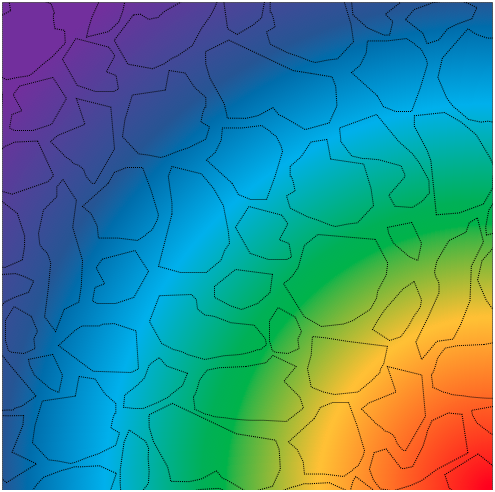
\includegraphics[width=0.8\linewidth]{figs/macro.png}
  \caption{Macroscale \(T_s\) distribution}
  \label{fig:mesoa}
\end{subfigure}
\begin{subfigure}{.485\textwidth}
  \centering
  
\includegraphics[width=0.8\linewidth]{figs/meso.png}
  \caption{Mesoscale surface BCs}
  \label{fig:mesob}
\end{subfigure}
\caption{Schematic of the (a) macroscale \gls{rev}-averaged solid surface temperature distribution and (b) the uniform surface temperature \gls{bc} on each mesoscale domain.}
\label{fig:meso}
\end{figure}

The spatial distribution of pebbles within the macroscale domain is usually unknown, so the use of the identical pebble representation in Figs. \ref{fig:mesoa} and \ref{fig:mesob} is purely pedagogical. Given the assumption of mesoscale periodicity, the solid surface temperature at each position \(\vec{x}\) in the macroscale domain represents a uniform surface temperature on a representative solid pebble centered at \(\vec{x}\).

In solid-fluid mixtures consisting of a homogeneous or multi-layer homogeneous solid phase, the heat equation may readily be applied to estimate the internal solid temperature distribution,

\beq
\label{eq:oem}
\rho_S C_{p,S}\frac{\partial T_S}{\partial t}-\nabla\cdot\left(k_S\nabla T_S\right)-\dot{q}_S=0\ ,
\eeq

\noindent where \(\rho_S\) is the solid density, \(C_{p,S}\) is the solid isobaric specific heat capacity, \(k_S\) is the solid thermal conductivity, \(T_S\) is the internal solid temperature, and \(\dot{q}_S\) is the volumetric heat source. The \(S\) subscript indicates that the thermal properties, volumetric heat source, and temperature correspond to the interior of the solid phase, and is distinct from the \(s\) subscript used to denote the intrinsic phase-averaged quantities in the macroscale solid energy conservation equations in Eqs.\ \eqref{eq:PSEnergy} and \eqref{eq:PSEnergy2}.

To reinforce the conceptual difference between \(s\) and \(S\) subscripts, consider a hypothetical pebble design consisting of three concentric layers of \gls{uo2}, helium, and zircaloy. Then, \(k_S\) might be specified as

\beq
k_S(r, T_S)=\begin{dcases}
k_{\text{UO}_2}(T_S) & r \leq r_1\\
k_{\text{helium}}(T_S) & r_1 < r \leq r_2\\
k_{\text{zircaloy}}(T_S) & r_2 \leq r < d_p/2\ ,
\end{dcases}
\eeq

\noindent where \(k_{\text{UO}_2}\), \(k_\text{helium}\), and \(k_\text{zircaloy}\) are temperature-dependent thermal conductivity correlations for each layer. The spatial dependence is listed in terms of the radial coordinate due to the uniform surface temperature \gls{bc} and interpretation of each representative pebble as a sphere with radius \(d_p/2\). \(r_1\) indicates the boundary between the \gls{uo2} and helium regions and \(r_2\) indicates the boundary between the helium and zircaloy regions. Similar piecewise expressions would be used for the heat source and the other properties of the solid. Conversely, properties with an \(s\) subscript differ are homogenized over the entire solid phase, which would be computed as some average of \(k_{\text{UO}_2}\), \(k_\text{helium}\), and \(k_\text{zircaloy}\).

Systems to which this multi-layer homogeneous solid modeling approach is readily applicable include homogeneous graphite pebbles commonly used near outer reflectors in \glspl{pbr} and conventional multi-layer pincell fuels in \glspl{lwr}. \gls{pbr} fuels, on the other hand, are extremely heterogeneous. Fig.\ \ref{fig:pbmr_pebble} shows a pictorial rendering of the fuel pebble design for the \gls{pbmr}, which is representative of many other \gls{pbr} fuels \cite{tecdoc1694}. The pebble consists of two main regions\mdash 1)~a central fuel-matrix region containing approximately 15,000 \glspl{cfp} randomly distributed in a graphite matrix and 2)~a homogeneous graphite shell. The micro length scale characterizes ``representative'' heterogeneous structures within the mesoscale domain; for application to the fuel-matrix region of \gls{pbr} fuels, these heterogeneous structures are the \glspl{cfp}.

Many other solid fuel forms encountered in nuclear applications share this heterogeneous character. \gls{fcm} fuels consist of conventional \glspl{cfp} dispersed in a \gls{sic} matrix and fabricated into cylindrical pellets that are intended to replace \gls{uo2} pellets in \glspl{lwr} \glspl{htgr} \cite{lu,snead_fcm}. For the conversion of research reactors from high- to low-enriched uranium, either the fuel loading or fissile atom density must be increased to retain the same reactor performance. As the size of the reactors are typically fixed, high fissile density dispersion fuels consisting of U$_3$Si$_2$ or UMo particles in an aluminum matrix have been used \cite{mistarihi,jeong2015}. A fast reactor fuel design consisting of metallic-coated fissile kernels surrounded by a fuel powder matrix has also been proposed \cite{abdalla}.

\begin{figure}[!h]
\centering
  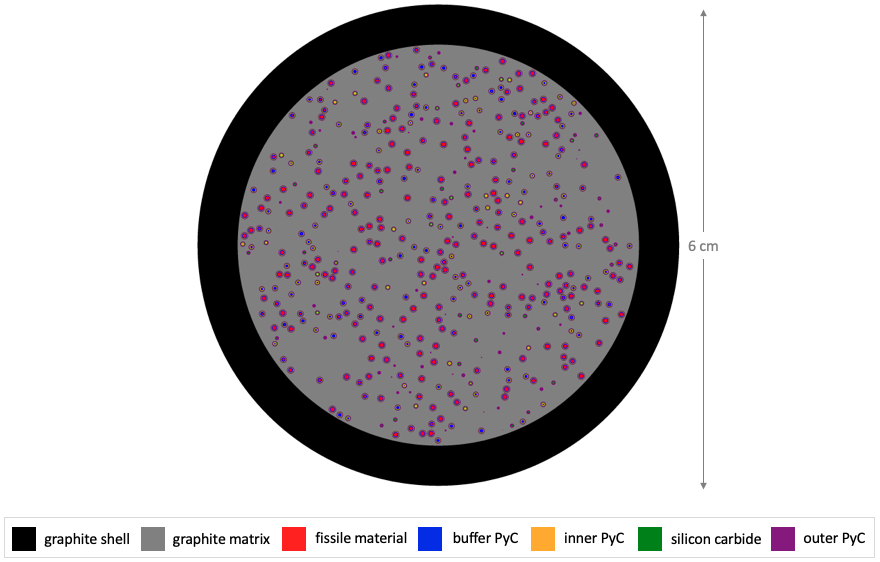
\includegraphics[width=0.85\linewidth]{figs/pbmr_pebble.png}
\caption{Schematic of the \gls{pbmr} fuel pebble design with colors indicating material composition.}
\label{fig:pbmr_pebble}
\end{figure}

The different material properties of the \gls{cfp} layers, combined with the localization of the fission heat source to the central \gls{cfp} kernel, makes Eq.\ \eqref{eq:oem} incapable to capturing the heat transfer in such a heterogeneous geometry. Rudimentary models based on volume-averaging the fuel-matrix properties and heat source as inputs to Eq.\ \eqref{eq:oem} may significantly underpredict fissile kernel temperatures \cite{brown_fcm,kamalpour, novak_2019}.

Multiscale analysis of heterogeneous solids is a large research field, especially in the analysis of conduction through composite materials; as such, a wide variety of methods have been proposed and used. A brief discussion of this research area provides larger context to this work. 

One obvious multiscale model is based on extending the \gls{rev} homogenization of a two-phase fluid-solid domain performed in Section \ref{sec:macro_deriv} to a two-phase soild-solid domain. By interpreting the continuous fluid phase as the solid matrix and the discrete solid pebble phase as the \glspl{cfp}, the spatially homogenized conservation equations in Eq.\ \eqref{eq:PorousEquations} also apply to the fuel-matrix region of \gls{pbr} fuels. For solid-solid domains, the velocity \(\vec{V}\) is zero such that closure requires specification of the volume fraction of the matrix phase, the effective matrix conductivity, the effective particle conductivity, and the interphase convective heat transfer coefficient. The latter three of these closures can be obtained as extensions of the models described in Sections \ref{sec:Kappa}, \ref{sec:KappaS}, and \ref{sec:alpha}, respectively. The models for \(\kappa_f\) are evaluated with zero thermal dispersion; the models for \(\kappa_s\) are evaluated with the assumption of a transparent solid matrix and no contact conduction component; and the models for \(\alpha\) are evaluated with zero Reynolds number. Other definitions for these closures from Monte Carlo simulations \cite{cho} or mixed diffusion kernels \cite{espinosa} have been proposed. 

A second method, referred to as ``multiscale expansion,'' expresses the temperature as a Taylor series expansion of successive corrections of order \(1\), \(\varsigma\), \(\varsigma^2\), \(\cdots\), where \(\varsigma\) is a small parameter. This ansatz is then plugged into the heat conduction equation and like terms collected to yield a separate differential equation for each correction \cite{weinan}. 

While the spatial homogenization is a natural companion to the macroscale porous media method, its implementation and use is considered as a future research activity. The multiscale expansion method, while mathematically rigorous, results in many unique physics kernels with low reuse potential in a modular computing framework. This method is therefore also not pursued further. The remainder of this section describes the two models investigated in this dissertation\mdash the \gls{hl} method and the \gls{hsd} method. Justification for their use over the macroscale homogenization and multiscale expansion methods is provided alongside a technical description.

\subsection{The Homogeneous Layers Method}

The \gls{hl} method blends aspects of a multilayer homogeneous solid that can be described by Eq.\ \eqref{eq:oem} with consideration of the \gls{cfp} layers thermal resistance and heat source localization. The \gls{hl} method is based on symmetrically smearing heterogeneities into a \gls{1d} multilayer solid while preserving volume fractions. Fig.\ \ref{fig:pbmr_hlm} shows one possible representation of the \gls{pbmr} pebble in Fig.\ \ref{fig:pbmr_pebble} with the \gls{hl} method. The total mass of each material is conserved and the geometric structure of the \glspl{cfp} is approximated as a multilayer spherical shell; 15,000 randomly-distributed particles have been simplified to a single pseudo-particle at the expense of a distortion in the thermal resistance seen by the kernel and the separation of a continuous matrix into isolated regions.

\begin{figure}[!h]
\centering
  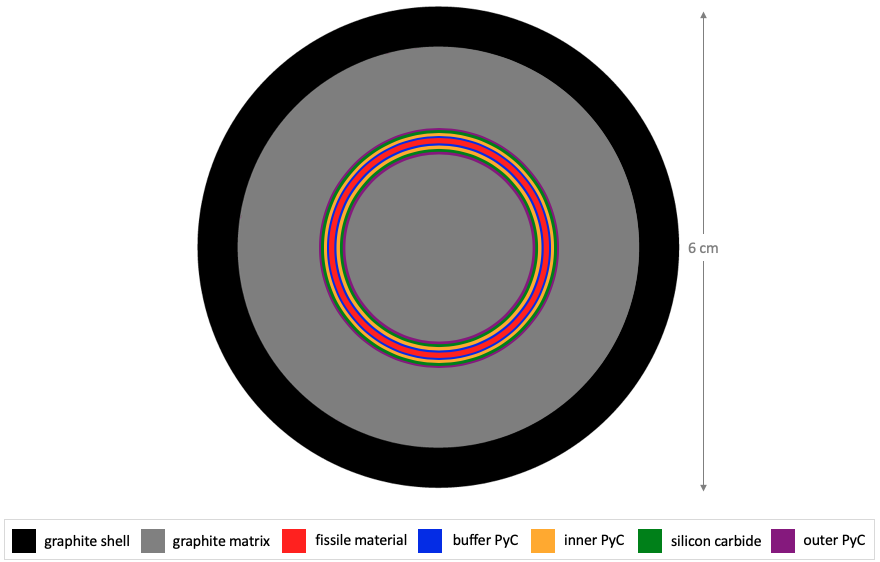
\includegraphics[width=0.85\linewidth]{figs/pbmr_hlm.png}
\caption{Schematic of the \gls{pbmr} fuel pebble design as represented by the \gls{hl} method; colors indicate different material compositions.}
\label{fig:pbmr_hlm}
\end{figure}

However, conserving volume fractions of the materials in the fuel-matrix region does not provide a sufficient number of constraints to determine 1)~the number of pseudo-particles, 2)~the location of the pseudo-particles, and 3)~the relative thicknesses of the ``inner'' and ``outer'' layers of non-kernel materials in the pseudo-particles. An infinite number of \gls{hl} representations of the pebble in Fig.\ \ref{fig:pbmr_pebble} can be conceived, so several additional requirements are arbitrarily imposed. 

The number of pseudo-particles \(N_p\) is the only free parameter. First, the fuel-matrix region is divided into \(N_p\) equal-volume spherical shells. Consider a shell spanning \(r_i\leq r\leq r_o\) with total volume \(\volume\) given as

\beq
\volume=\frac{4}{3}\pi\left(r_o^3-r_i^3\right)\ .
\eeq

\noindent For a \gls{cfp} \gls{pf} in the fuel-matrix region of \(\epsilon_\text{cfp}\), \(1-\epsilon_\text{cfp}\) of the shell volume is matrix material. The thickness of the matrix layer along the inner surface, or \(\delta_i\), is chosen such that half of the matrix material is present in a layer along the inner surface. Likewise, the thickness of the matrix layer along the outer surface, or \(\delta_o\), is chosen such that half of the matrix material is present in a layer along the outer surface. In other words, the inner matrix layer thickness is calculated as

\beq
\frac{4}{3}\pi\left\lbrack\left(r_i+\delta_i\right)^3-r_i^3\right\rbrack=\frac{1}{2}\left(1-\epsilon_\text{cfp}\right)\volume\ ,
\eeq

\noindent while the outer matrix layer thickness is calculated as

\beq
\frac{4}{3}\pi\left\lbrack r_o^3-\left(r_o-\delta_o\right)^3\right\rbrack=\frac{1}{2}\left(1-\epsilon_\text{cfp}\right)\volume\ .
\eeq

\noindent A similar process is then performed for the materials in the \gls{cfp}, where the \gls{pf} of each material in the \gls{cfp} is used to determine the relative volume occupied in the segment.

The \gls{hl} method has no direct correlation to the actual geometry, and temperature solutions should only be used to predict integral metrics such as maximum and average material-wise temperatures. However, the \gls{hl} method is considered here for two reasons \mdash1)~the method is simple to implement and representative of the limitations in single-\gls{pde} fuel models used in many legacy \gls{th} tools; and 2)~the \gls{hl} method has recently been used in preliminary steady-state modeling of \gls{fcm} fuels \cite{brown_fcm} and transient analysis of the Mark-1 \gls{pbfhr} \cite{xin_wang_thesis} that is the subject of the modeling in Chapter \ref{sec:pbfhr}.

\subsection{The Heat Source Decomposition Method}

The second multiscale model considered is the \gls{hsd} method, which is based on the concept of superposition solutions to linear differential equations \cite{stainsby}. If the heat equation is linear, it may be split into different models for the meso and micro length scales that are superimposed to obtain an approximate temperature solution. A description of the \gls{hsd} method begins by splitting the heterogeneous heat source \(\dot{q}\) into an average \(\la\dot{q}\ra\) and a fluctuation \(\hat{\dot{q}}\),

\beq
\label{eq:heat_source_decomp}
\dot{q}=\la\dot{q}\ra+\hat{\dot{q}}\ ,
\eeq

\noindent where the average of the fluctuation is zero. Each heat source on the \gls{rhs} of Eq.\ \eqref{eq:heat_source_decomp} is used in a separate conduction equation. The conduction equation based on the average heat source is referred to as the ``mesoscale'' model,

\beq
\label{eq:MesoscaleSolution}
\rho_\text{meso} C_{p,\text{meso}}\frac{\partial T_\text{meso}}{\partial t}-\nabla\cdot(k_\text{meso}\nabla T_\text{meso})-\la\dot{q}\ra=0\ ,
\eeq

\noindent \(\rho_\text{meso}\), \(C_{p,\text{meso}}\), and \(k_\text{meso}\) represent the thermal properties of the heterogeneous domain homogenized in space according to various mixing approaches described in Section \ref{sec:ClosuresMesoMicro}. The mesoscale temperature \(T_\text{meso}\) represents the long-wavelength thermal solution due to the average heat source and average properties. Note that Eq.\ \eqref{eq:MesoscaleSolution} is very similar to the multi-layer homogeneous solid model in Eq.\ \eqref{eq:oem}, except that all thermal properties are spatially homogenized and the heat source is averaged over the domain.

The conduction equation based on the fluctuating heat source is referred to as the ``microscale'' model,

\beq
\label{eq:MicroscaleSolution}
\rho_\text{micro} C_{p,\text{micro}}\frac{\partial T_\text{micro}}{\partial t}-\nabla\cdot(k_\text{micro}\nabla T_\text{micro})-\hat{\dot{q}}=0\ ,
\eeq

\noindent \(\rho_\text{micro}\), \(C_{p,\text{micro}}\), and \(k_\text{micro}\) represent the thermal properties resolved on the fine scale; an \(S\) subscript instead of the ``micro'' subscript would also have been appropriate. The microscale temperature \(T_\text{micro}\) represents the small-scale correction to the mesoscale solution.

The approximate temperature solution in the interior solid domain is the superposition of the two solutions,

\beq
\label{eq:MultiscaleSolution}
T_S(\vec{x})=T_\text{meso}(\vec{x})+\sum_{i=1}^{n_p}T_{\text{micro},i}(\vec{x}_i)\ ,
\eeq

\noindent where the summation over the number of \glspl{cfp} \(n_p\) indicates that the microscale solution \(T_{\text{micro},i}\) for the \(i\)-th particle is translated to the location \(\vec{x}_i\) corresponding to the center of that particle. If pebble self-shielding effects are neglected such that the heat source in each particle is identical, a microscale model may be constructed for a single particle and translated to each of the \(n_p\) locations. This simplification is assumed throughout, though it is not an inherent limitation of the method. 

In summary, application of the \gls{hsd} method to the \gls{pbmr} pebble in Fig.\ \ref{fig:pbmr_pebble} involves the following calculation steps\mdash 

\begin{enumerate}
\itemsep0.3em
\item Decompose the heat source into an average and a fluctuation according to Eq.\ \eqref{eq:heat_source_decomp}.
\item Solve the mesoscale model in Eq.\ \eqref{eq:MesoscaleSolution} over the entire fuel-matrix region and subject to the \glspl{bc} described in Section \ref{sec:BCsMesoMicro}.
\item Solve the microscale model in Eq.\ \eqref{eq:MicroscaleSolution} over a single average \gls{cfp} and subject to the \glspl{bc} described in Section \ref{sec:BCsMesoMicro}.
\item Translate the microscale solution to the locations of the 15,000 \glspl{cfp} and add to the mesoscale solution according to Eq.\ \eqref{eq:MultiscaleSolution}.
\end{enumerate}

An in Section \ref{sec:verification_meso} provides a more intuitive grasp of the method. The \gls{hsd} method is considered here due to successful application to cylindrical \gls{cfp} compacts that share many similarities to \gls{pbr} fuels \cite{stainsby}.

In practice, the location of each \gls{cfp} is unknown, preventing prediction of the temperature at a specific location. However, often of greater practical interest is the estimation of integral metrics such as maximum and material-wise averaged temperatures. Even if the locations of the heterogeneities are unknown, provided the \glspl{cfp} are randomly dispersed through the domain, the maximum and minimum temperatures in material \(i\) can be approximated as

\beq
\label{eq:MaxT}
\text{max}\left(T_{i}\right)= \text{max}\left(T_\text{meso}\right)+\text{max}\left(T_{\text{micro},i}\right)\ ,
\eeq

\beq
\label{eq:MinT}
\text{min}\left(T_{i}\right)= \text{min}\left(T_\text{meso}\right)+\text{min}\left(T_{\text{micro},i}\right)\ .
\eeq

\noindent In other words, maximum and minimum temperatures are evaluated assuming a microscale domain is situated precisely at the location of the maximum and minimum mesoscale temperatures, respectively. This provides the bounding maximum and minimum temperatures for material \(i\), and hence the actual maximum and minimum temperatures will be within this range given the limitations of the mixing methods used for mesoscale material properties.

In addition, if the mesoscale temperature solution varies over a longer length scale than the size of the \glspl{cfp}, the average temperature in material \(i\) can be approximated as

\beq
\label{eq:AvgT}
\la T_i\ra=\la T_\text{meso}\ra+\la T_{\text{micro},i}\ra\ .
\eeq

\noindent Note that while Eq.\ \eqref{eq:ConstantShiftMMD} requires the average of the microscale solution over the entire microscale domain to be zero, the $i$ subscript in Eq.\ \eqref{eq:AvgT} represents the average over only the $i$-th material layer in the microscale domain. The approximation in Eq.\ \eqref{eq:AvgT} is frequently applicable to \gls{pbr} fuels because the micro length scale is approximately 50 times smaller than the meso length scale, and extremely different particle-to-particle powers or non-uniform matrix-shell \glspl{bc} are uncommon.

The most important assumption made in the \gls{hsd} method is that the heat equation is linear, and thus amenable to superposition techniques. Linearity implies that the thermal properties are independent of temperature. In this research, the meso and micro scale models are applied to steady-state analysis of the Mark-1 \gls{pbfhr}. The \gls{pbfhr} core temperature rise of 100\si{\celsius}, the close proximity of the \glspl{cfp} to the pebble surface, and the distribution of the pebble power among a relatively high number of \glspl{cfp} per pebble result in pebble temperature distributions that vary relatively little throughout the bed as compared to other nuclear fuels such as \gls{uo2} pellet fuels. 

Based on the solid properties provided in Appendix \ref{sec:props}, a \(\pm\)100\si{\celsius} change in temperature relative to 800\si{\celsius} results in approximately a \(\mp\)5\%, \(\mp\)10\%, and \(\mp\)10\% change in the matrix graphite, \gls{uo2}, and \gls{sic} thermal conductivities, respectively. To the author's knowledge, temperature-dependent models are unavailable for porous and pyrolitic graphite. These relatively small variations with temperature justify the use of thermal properties evaluated at the bed-averaged temperature.

Transient modeling, especially in scenarios with large power changes such as \glspl{ria}, must consider temperature dependence. There are a number of ways in which some property temperature dependence can be retained. The \gls{hsd} method can be applied iteratively in a number of discrete heterogeneous regions, each with unique thermal properties evaluated at the average temperature of the region. Or, unique thermal properties may be used for each pebble according to its location in the macroscale solid temperature field. Future work will incorporate temperature dependence in the \gls{hsd} method.

In most \glspl{pbr}, of equal or greater concern is the dependence of thermal properties on burnup. This dependence can be easily accommodated provided the burnup over a pebble is assumed uniform by using constant thermal properties evaluated at a particular burnup level.

\subsection{Boundary and Initial Conditions}
\label{sec:BCsMesoMicro}

Most \gls{pbr} fuels contain a surface layer of homogeneous graphite to protect the fuel-matrix region from erosion. The surface temperature of a representative pebble in each computational element is taken as the average macroscale solid surface temperature over the element, or \(T_{s,\text{avg}}\). The \gls{hl} method is applied over both the heterogeneous fuel-matrix region and the homogeneous graphite shell, so a temperature \gls{bc} on the pebble surface \(\Gamma_p\) is specified as

\beq
\label{eq:PebSurf}
T_S\rvert_{\Gamma_p}=T_{s,\text{avg}}\ .
\eeq

\noindent The \gls{hsd} method involves coupled solutions on two length scales and summing those solutions together as in Eq.\ \eqref{eq:MultiscaleSolution}. Unlike the \gls{hl} method, the \gls{hsd} method is only applied in heterogeneous regions. In the homogeneous graphite shell, the temperature distribution is obtained by solution of Eq.\ \eqref{eq:oem} with surface \gls{bc} given by Eq.\ \eqref{eq:PebSurf}. At the interface between the homogeneous shell and the fuel-matrix region, continuity of temperature and heat flux with the homogeneous shell is required.

\begin{comment}
\beq
\label{eq:MesoShift}
\left(T_\text{meso}+T_\text{micro}\right)\rvert_{\Gamma_i}=T_S\rvert_{\Gamma_i}\ ,
\eeq

\beq
\label{eq:MesoShift2}
\left(-k_\text{meso}\nabla T_\text{meso}\cdot\hat{n}-k_\text{micro}\nabla T_\text{micro}\cdot\hat{n}\right)\rvert_{\Gamma_i}=-k_S\nabla T_S\cdot\hat{n}\rvert_{\Gamma_i}\ .
\eeq
\end{comment}

In addition, the microscale solution must have a zero average over the microscale domain in order to represent a zero-average fluctuation on the long-wavelength mesoscale solution. This is enforced by applying a Dirichlet \gls{bc} on the boundary \(\Gamma_\text{micro}\) of the microscale domain such that the average of the microscale solution over the microscale volume \(\volume_\text{micro}\) is zero,

\beq
\label{eq:ConstantShiftMMD}
T_\text{micro}\rvert_{\Gamma_m} =-\frac{1}{\volume_\text{micro}}\int_{\volume_\text{micro}} T_\text{micro}d\volume\ .
\eeq

\subsection{Closures}
\label{sec:ClosuresMesoMicro}

This section describes models used for the meso and micro scale closures. Section \ref{sec:micro_props} describes models for the locally resolved properties \(\rho_\text{micro}\), \(C_{p,\text{micro}}\), and \(k_\text{micro}\), while Section \ref{sec:meso_props} describes models for the spatially homogenized mesoscale properties \(\rho_\text{meso}\), \(C_{p,\text{meso}}\), and \(k_\text{meso}\).


\subsubsection{Microscale Solid Properties}
\label{sec:micro_props}

Both the \gls{hl} and \gls{hsd} methods require the internal solid properties \(\rho_S\), \(C_{p,S}\), and \(k_S\) for closure; in the context of the \gls{hsd} method, these properties have been represented equivalently with the notation \(\rho_\text{micro}\), \(C_{p,\text{micro}}\), and \(k_\text{micro}\). Correlations for density, isobaric specific heat, and thermal conductivity of pure, un-mixed, solid materials as a function of internal solid temperature is provided in Appendix \ref{sec:props}.

\subsubsection{Mesoscale Solid Properties}
\label{sec:meso_props}

The spatially homogenized properties \(\rho_\text{meso}\), \(C_{p,\text{meso}}\), and \(k_\text{meso}\) represent effective properties of a heterogeneous solid. The homogenization models described in this section assume that these effective properties are a combination of the properties of its constituents.

Consider a mixture of materials \(i\) for \(i=1\ ...\ N_m\) each with a phase fraction \(\epsilon_i\) and generic property \(\chi_i\). These phase fractions sum to unity. The simplest method for determining average properties is the use of series combination,

\beq
\label{eq:series}
\chi=\sum_{i\ =\ 1}^{N_m}\epsilon_i\chi_i\ ,
\eeq

\noindent which is equivalent to a volume average. Alternatively, a parallel combination may be used,

\beq
\label{eq:parallel}
\frac{1}{\chi}=\sum_{i\ =\ 1}^{N_m}\frac{\epsilon_i}{\chi_i}\ .
\eeq

\noindent Specifically for binary systems such as the particle-matrix system, many theoretical models based on the notion of transport have been developed. Chiew and Glandt extended Maxwell's potential theory for randomly-distributed, non-interacting, spheres \cite{progelhof} to higher order, giving

\beq
\label{eq:ChiewGlandt}
\chi=\chi_c\frac{1+2\beta_n\epsilon_d+\left(2\beta_n^3-0.1\beta_n\right)\epsilon_d^2+0.05\epsilon_d^3\exp{(4.5\beta_n)}}{1-\beta_n\epsilon_d}\ ,
\eeq

\noindent where \(\beta_n\) is defined as

\beq
\label{eq:betanDef}
\beta_n\equiv\frac{\chi_d-\chi_c}{\chi_d+2\chi_c}\ ,
\eeq

\noindent and \(c\) subscripts indicate the continuous phase and \(d\) subscripts indicate the dispersed phase \cite{kamalpour,liu,gonzo,folsom}. Lewis and Nielsen developed a similar extension to Maxwell's theory as \cite{nielsen,progelhof}

\beq
\label{eq:Nielsen}
\chi=\chi_c\frac{1+1.5\beta_m\epsilon_d}{1-\beta_m\epsilon_d\left(1+\frac{1-0.637}{0.637^2}\ \epsilon_d\right)}\ ,
\eeq

\noindent where \(\beta_m\) is defined as

\beq
\label{eq:BmDef}
\beta_m\equiv\frac{\chi_d-\chi_c}{\chi_d+1.5\chi_c}\ .
\eeq

\noindent For solids with multiple layers of heterogeneity, such as most \gls{pbr} fuels, properties are first homogenized beginning on the fine scales and then on increasingly coarse scales. In this work, either Eq.\ \eqref{eq:ChiewGlandt} or Eq.\ \eqref{eq:Nielsen} is used for averaging the fuel matrix with the \glspl{cfp}, while either Eq.\ \eqref{eq:series} or Eq.\ \eqref{eq:parallel} are used for all other averages. 

Take the \gls{pbmr} pebble in Fig.\ \ref{fig:pbmr_pebble} as an example, with Eq.\ \eqref{eq:series} used for all averages except the \glspl{cfp} with the matrix. The intrinsic phase average of a property \(\chi\) over the pebble is calculated as

\beq
\label{eq:NonTransport2}
\chi_s= \epsilon_\text{fm}\chi_\text{fm}+(1-\epsilon_\text{fm})\chi_\text{gs}\ ,
\eeq

\noindent where \(\epsilon_\text{fm}\) is the volume fraction of the pebble that is the fuel-matrix region, \(\chi_\text{fm}\) is the average of \(\chi\) over the fuel-matrix region, and \(\chi_\text{gs}\) is the property of the graphite shell. \(\chi_\text{fm}\) is calculated as

\beq
\label{eq:NonTransport}
\chi_\text{fm}= \epsilon_\text{cfp}\chi_\text{cfp}+(1-\epsilon_\text{cfp})\chi_\text{mat}\ ,
\eeq

\noindent where \(\epsilon_\text{cfp}\) is the volume fraction of the fuel-matrix region that is \glspl{cfp}; \(\chi_\text{cfp}\) is the average of \(\chi\) over a \gls{cfp} using the series average in Eq.\ \eqref{eq:series}; and \(\chi_\text{mat}\) is the property of the matrix. 

For \gls{pbr} applications, the mesoscale properties indicated generically by \(\rho_\text{meso}\), \(C_{p,\text{meso}}\) and \(k_\text{meso}\) are equivalent to \(\rho_\text{fm}\), \(C_{p,\text{fm}}\) and \(k_\text{fm}\). The intrinsic solid phase-averaged properties \(\rho_s\), \(C_{p,s}\), and \(k_s\) required in the macroscale model are computed using these homogenization models over the entire pebble.

\section{Limitations, Assumptions, and Knowledge Gaps}
\label{sec:MacroAssumptions}

Many assumptions were made explicitly or implicitly in the derivation of the macroscale spatially homogenized conservation equations in Section \ref{sec:macro_deriv} and in the models selected for the meso and micro length scales in Section \ref{sec:mesomicro}. Assumptions have been made in 1)~the form of the local conservation equations in Eqs.\ \eqref{eq:ContinuityNonPorous}--\eqref{eq:EnergyNonPorous} and \eqref{eq:InternalEnergy}, 2)~in the spatial homogenization procedure used to obtain the macroscale model in Eqs.\ \eqref{eq:PorousEquations} and \eqref{eq:PrimitiveEqns}, and 3)~in the implementation details of the \gls{hl} and \gls{hsd} methods. Existing closure models applicable to \glspl{pbr} also exhibit many limitations and knowledge gaps at all three length scales. A brief summary is now provided of the limitations, assumptions, and knowledge gaps that have the largest impact on the general applicability of this multiscale method to modeling of \glspl{pbr}.

Both the local mass conservation in Eq.\ \eqref{eq:ContinuityNonPorous} and the two-phase homogenization assume a single phase fluid and no mass transfer between the fluid and solid phases. The macroscale model therefore cannot model multi-phase fluid flow, such as water ingress events important to safety analysis of \glspl{htgr}. The assumption of a pure, simple, fluid in the conservation of energy equations excludes analysis of reacting flows. The macroscale \glspl{bc} assume the flow is subsonic. 

There are several inherent limitations of the macroscale modeling approach with regards to predicting key safety metrics such as maximum fuel temperature. Because porous media models are based on spatial averaging, all local flow and heat transfer effects are only retained in an average sense. The distribution of temperature on an individual pebble surface or reflector block is unknown. Resolved \gls{cfd} simulations of pebbles show that surface temperatures are tens to hundreds of degrees higher, depending on the flow conditions, at stagnation points and near the low-flow recirculation regions behind pebbles than near thin, main-flow aligned, gaps \cite{bai,ferng,ge,lee2007,song,wu2010}. This surface temperature distribution affects the maximum fuel temperature, but the macroscale model is restricted to predicting the meso and micro scale temperatures based on a surface-uniform solid temperature, and hence will underpredict the true maximum fuel temperature. \gls{cfd} simulations of fluid flow around pebbles with the \glspl{cfp} resolved within each pebble are required to estimate the extent to which a uniform pebble surface temperature underpredicts the true maximum fuel temperature. The large temperature margins to \gls{cfp} failure often permit the use of safety factors to conservatively account for this effect. However, reactors with higher power densities and operating temperatures may have smaller margins to failure and require more refined analysis.

Chemical reactions are frequently strong functions of temperature. In addition to underpredicting the true maximum fuel temperature, the homogenization of the pebble surface temperature will underpredict the variation in chemical reaction rates over the surface of a pebble. For example, Fig.\ \ref{fig:corroded_pebble} shows a graphite pebble, originally spherical in shape, with significant and nonuniform oxidation that may have been caused by nonuniform surface temperature distributions. Similar stagnation-related chemical reactions have resulted in coolant polymerization in organic-cooled reactors \cite{shirvan}. Extensive dimensional changes may result in further amplification of surface temperature non-uniformity and complicate pebble handling systems. 

Spatial homogenization may also fail to correctly capture mass transfer processes such as tritium uptake in the pebbles of lithium-bearing salt-cooled systems. Further investigation is needed to better understand the effect of spatial homogenization on prediction of integral chemical reaction and mass transfer rates.

% Stagnation points usually occur at or near the pebble contact points that are not aligned with the flow direction due to vortex formation and back flow \cite{lee_lee, hassan, ge,king}. Nusselt numbers typically range between 10 and 150 over the surface of a single pebble \cite{ferng}.

\begin{figure}[!h]
\centering
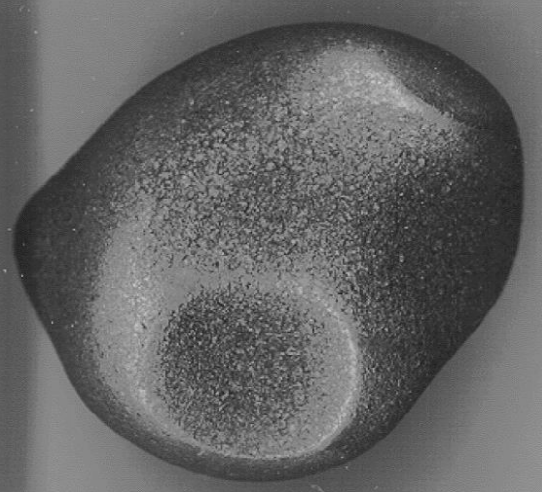
\includegraphics[width=0.4\linewidth]{figs/corroded_pebble.png}
\caption{Corroded graphite pebble, originally spherical in shape, with nonuniform oxidation damage from the KFA Veluna experiment \cite{hassan_mev}.}
\label{fig:corroded_pebble}
\end{figure}

%Provided the neutron migration length is larger than the porous media averaging length, the use of a porous media \gls{th} solution for temperature feedback in neutronics simulations is an acceptable simplification of the fluid flow and heat transfer \cite{aufiero_2016, rintala}.

In addition to the assumptions and limitations inherent in the macroscale model, the existing literature on macroscale closures is characterized by many knowledge gaps that affect the applicability of this form of multiscale analysis to \glspl{pbr}. The remainder of this section highlights several of these gaps in order to motivate future experimental programs aimed at closure refinement. Most of the emphasis is placed on the interphase friction factor \(W\), interphase convective heat transfer coefficient \(\alpha\), and effective solid thermal conductivity \(\kappa_s\), rather than on the porosity \(\epsilon\), Brinkman viscosity \(\tilde{\mu}\), and effective fluid thermal conductivity \(\kappa_f\). This emphasis is justified because the field of \gls{dem} modeling is well-established and equipped with methods for predicting porosity in complex domains, provided accurate data is available for pebble material properties such as roughness and elastic modulus \cite{lammps,openfoam,liggghts,zhang2001}. However, the assumption of a time-independent porosity precludes analysis of large-motion events such as earthquakes, and future work may incorporate \gls{dem} modeling to obtain more accurate predictions of porosity. Further, the Brinkman viscosity and effective fluid thermal conductivity are seldom used in modeling of \glspl{pbr}, and flow and temperature predictions are relatively insensitive to their selection \cite{auwerda_2011,tecdoc1163}.

Generally speaking, models for \(W\), \(\alpha\), and \(\kappa_s\) are based on experimental data measured at the inlet and outlet of a bed. For example, a model for \(W\) would be developed by fitting pressure drop data obtained as differences between the inlet and outlet pressure along the centerline of a pipe containing a packed bed. The most significant knowledge gap for macroscale closures is the lack of a spatial dependence that explicitly considers the very different \gls{th} effects in the near-wall versus bulk regions of the bed. The porosity that appears in these closure models represents the bed-averaged porosity. A common, but crude, approximation attempts to extend bulk bed correlations to the near-wall regions by interpreting the porosity as the local porosity \cite{kaviany, vortmeyer, giese, vafai}. However, many of the macroscale closures predict unphysical behavior as porosity tends to unity. For example, the hydraulic diameter in Eq.\ \eqref{eq:Dh} and \(\kappa_\text{radiation}\) in Eq.\ \eqref{eq:KappaRadiationBB} both tend to infinity.

As discussed in greater detail in Chapter \ref{sec:sana}, the lack of models correlated for the near-wall region may contribute to significantly higher errors in temperature predictions in these regions \cite{novak_2019}. Experimental and numerical investigations are required to develop macroscale closures applicable to the near-wall region, as well as supporting parameters such as the hydraulic diameter. The \gls{neams} funding call in 2019 titled ``Near-Wall Gas-Flow Correlations in Pebble Bed Reactors'' points to the importance of addressing this knowledge gap for \gls{pbr} thermal analysis \cite{neams2}. 

Even in the bulk region, a number of important assumptions have been made. The model for \(\kappa_\text{radiation}\) in Eq.\ \eqref{eq:KappaRadiationBB} applies to a transparent fluid. While many pure salts are broadly transparent, absorption coefficients may be five times higher upon the addition of impurities such as chromium \cite{chaleff}. In addition, few macroscale closure models consider any entrance length effects, and inconsistencies are commonly observed in proposed modifications for entrance regions. For example, the Nusselt number is generally larger in the first few sphere layers because of thinner boundary layers \cite{ferng,song}. However, others have observed the opposite \cite{KTAhtc} or no effect \cite{song}, which may be attributable to differences in packing structure and the counteracting effect of absent turbulent wakes from upstream pebbles \cite{achenbach}. 

At the meso and micro length scales, the heterogeneous pebble geometry has been dramatically simplified through either the \gls{hl} or \gls{hsd} method. In this dissertation, the effect of self-shielding on \gls{cfp} power distribution has been neglected, and thermal properties in the \gls{hsd} are assumed independent of temperature. 

Finally, all three length scales are affected by uncertainties in fundamental fluid and solid properties, as well as in their effective mixed state. The strong dose dependence on graphite properties is neglected \cite{seker}, and the dependence of \gls{cfp} layer properties on manufacturing conditions is not considered. In the mixing of component properties to estimate effective properties, it is assumed that the properties of an individual component in a mixture are the same as the properties of the corresponding pure material. This simplification neglects differences in microstructure between the pure components and the mixture, which can be significant in graphite and \gls{fcm} fuels \cite{folsom,lee2017}.


% TODO: literature review of CFD of pebble beds
\begin{comment}


Most experiments and simulations show a higher pressure drop per unit length in the first several sphere layers than in the bulk \cite{baker_2010}, though others have not observed any entrance region effect \cite{calis,bai_2009,zhang2016}. 

These different reported entrance effects for Nusselt number and friction factor remain to be reconciled as functions of packing and flow regime.

%\cite{bai} fits drag with polynomial in Re, gives bad results at high Re
\end{comment}

% uncertainties in the correlations
%Maximum temperatures are in some cases very sensitive to the models used for \(\kappa_s\) \cite{sana_report,becker}. Contributing to this sensitivity are the relatively high uncertainties reported in many experimental measurements, which may be partially attributable to the sensitivity of contact conduction to corrosion \cite{aichlmayr}, the sensitivity of the thermal conductivity to the oxidation state \cite{swift}, and/or the presence of small convection currents \cite{nozad}.



\chapter{Pronghorn: Software for Multiscale Analysis}
\label{sec:ph}

The tightly-coupled multiscale and multiphysics nature of \glspl{pbr}, the importance of \gls{3d} unstructured meshing capabilities, and the restrictive emphasis of earlier modeling tools on gas coolants motivates the development of a new modeling tool in this research to enable application of the models described in Chapter \ref{sec:PhysicalModels} to multiscale analysis of single-phase \glspl{pbr}. This new application, Pronghorn, is a multi-dimensional, coarse-mesh, reactor analysis tool intended to accelerate the design and analysis cycle for \glspl{pbr} with computing requirements within reach of industry and regulatory stakeholders. 

Multiscale analysis at its core is a form of multiphysics analysis\mdash a set of models are coupled together to account for physics feedback effects between various length scales. The key functional requirements in the development of new \gls{pbr} multiscale simulation capabilities are 1)~tightly-coupled solution and data transfer schemes between multiple physics and length scales relevant to nuclear reactors, 2)~efficient simulation on unstructured meshes, and 3)~flexible source code modification to include closures for non-gas coolants. Additionally, new capabilities should be developed with the goal of enhancing modeling tools available to the nuclear engineering community and designed with reuse and longevity in mind.

Many commercial \gls{cfd} applications such as COMSOL and FLUENT include porous media models for fluid flow on unstructured meshes with capacity for user-defined closures and native multiphysics coupling with other physics domains \cite{comsol_cfd,fluent}. However, neutron transport physics, perhaps the most important feedback effect on \gls{th} physics, are often not available in these commercial applications due to export control regulations. While most commercial \gls{cfd} tools include a model builder for implementation of user-defined \glspl{pde}, individual efforts in this area are difficult to reuse across multiple research groups and institutions and often require custom-built testing systems to ensure high software quality. For example, a number of research groups have separately implemented deterministic neutron transport models into local COMSOL license checkouts, duplicating many person-hours of effort that could have been avoided through the use of existing neutron transport solvers \cite{xin_wang,hurt,chandler,xoubi,fiorina}. The heavy use of empirical models for fission gas buildup and irradiation-induced microstructural changes in nuclear materials modeling makes implementation of this second important physics domain in commercial \gls{cfd} tools an additional challenge to comprehensive multiphysics analysis for \glspl{pbr}. Difficulty parallelizing user-defined functions has in some cases restricted these types of software development to serial implementations \cite{becker}.

Commercial applications are also usually closed source, complicating or precluding the adjustment of the numerical solution procedure or physics model. For instance, implementation of acceleration methods to achieve robust numerical performance for neutron transport simulations of a wide range of nuclear systems \cite{willert} may be challenging. The closed source nature of commercial tools is likely a primary motivation for the previously-cited researchers resorting to implementation of deterministic transport models in COMSOL as opposed to coupling an existing tool to COMSOL. The combination of license costs in the thousands to tens of thousands of dollars range, closed source code, and difficulty distributing new physics capabilities within the nuclear engineering community prompt alternative strategies for numerical implementation of the models in Chapter \ref{sec:PhysicalModels}.

Within the nuclear engineering field, several non-commercial tools exist for modeling \gls{pbr} \gls{th}. Examples of these tools include the German Forschungszentrum J{\"u}lich Research Centre THERMIX application, widely used in the design and analysis of \glspl{pbr} in Germany and South Africa \cite{gao,tecdoc1163,THERMIX, zwaan}; the University of Michigan and \gls{nrc} \gls{agree} application frequently applied to prismatic gas reactor analysis \cite{seker}; the \gls{kaeri} GAMMA application \cite{lim}; the Rensselaer Polytechnic Institute \gls{pebfd} application \cite{y_li}; and the Iranian Sharif University of Technology \gls{thpp} application \cite{nouri}.

A significant limitation of many of these tools is the use of structured meshes that are frequently also restricted to \gls{2d} $r$-$z$ geometries. Unstructured meshes are necessary for representing the diverging and converging cones common to many \gls{pbr} beds, while \gls{3d} geometries are needed to capture asymmetric power profiles, \glspl{bc}, and transients such as control rod ejection. THERMIX and \gls{thpp} only include a friction-dominated model, and may not be capable of accurately simulating plena or high-Reynolds number flows. Several applications are also restricted to the ideal gas \gls{eos} for fluid properties, preventing simulation of salt-cooled systems. 

While modifying one or more of these tools to solve the multiscale models in Chapter \ref{sec:PhysicalModels} on a \gls{3d} unstructured mesh is certainly an option, the age of many of the applications may make source code changes and maintenance challenging. Further, modification of one of these tools does not directly address the objective of tightly-coupled solution and data transfer with other physics domains relevant to \glspl{pbr}. For these reasons, development of a new application, Pronghorn, on an existing and modern multi-application computing framework is the best approach to meet the key design objectives of tightly-coupled multiphysics, unstructured meshing, and source flexibility. For reasons to follow, the \gls{moose} framework is selected as the base computing platform for the present work.

\gls{moose} is an open source, distributed- and shared-memory parallel, \texttt{C++} \gls{fe} framework developed by \gls{inl} that enables tightly-coupled implicit solution of nonlinear equations \cite{gaston,moose}. \gls{moose} enables practitioners familiar with the applied math aspects of their application areas to translate those concepts into portable, extensible, and high performance software in a method similar to other general purpose toolkits such as deal.II \cite{dealII91} and OpenFOAM \cite{openfoam}. The \gls{moose} framework combines the LibMesh \gls{fe} library \cite{libMeshPaper} with the nonlinear solution and preconditioning capabilities of the \gls{petsc} together in a modular structure to allow rapid production of new simulation tools. 

The use of a \gls{fe} spatial discretization permits the use of unstructured meshes based on a wide variety of element types, and the \gls{parmetis} library provides \gls{mpi}-based mesh partitioning, while LibMesh provides \gls{amr}. \gls{moose} simulations have demonstrated scalability to over 30,000 cores \cite{kong}. Nonlinear solution is based on the \gls{jfnk} method with Jacobians that can optionally be calculated by \gls{ad} to greatly reduce application development time and improve numerical convergence. 

A simulation tool built on the \gls{moose} framework is referred to as an ``application.'' The hierarchical design and common class inheritance permit in-memory multiphysics coupling of these applications to enable prediction of complex interacting phenomena. Fig. \ref{fig:moose_apps} shows a hierarchical depiction of all of the applications tracked by \gls{moose}'s \gls{ci} system and their relationships to one another \cite{moose_training}. Text within rectangular boxes are the names of \gls{moose} applications, while an arrow pointing from box \(A\) to box \(B\) indicates that application \(A\) depends upon, or ``consumes'' application \(B\). The applications shown in the boxes are a mix of physics modules and fluid property implementations. All applications depend upon the \gls{moose} framework, which consists of the framework and open source physics modules listed at the bottom of the \gls{moose}-labeled rectangle.

\begin{figure}[!h]
  \centering
  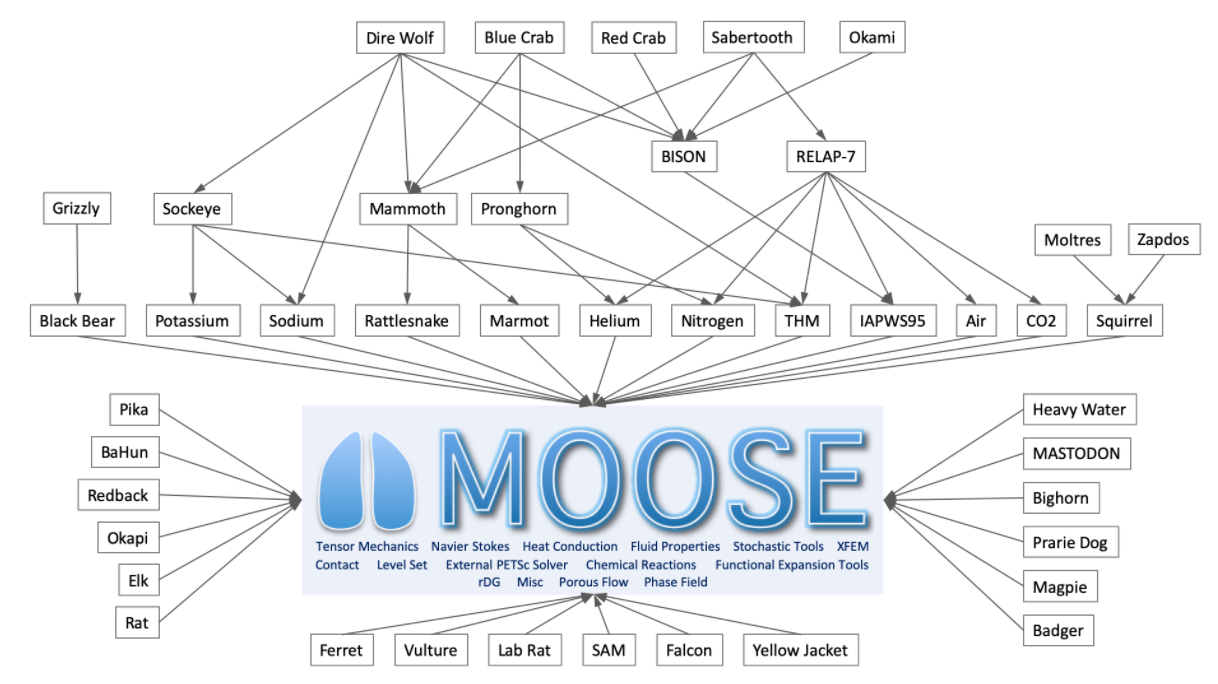
\includegraphics[width=0.9\linewidth]{figs/moose_apps.png}
  \caption{Hierarchical summary of all applications tracked by \gls{moose}'s \gls{ci} system and their relationships to one another \cite{moose_training}.}
\label{fig:moose_apps}
\end{figure}

Examples of applications in the nuclear engineering space include Rattlesnake neutron transport \cite{rattlesnake}; BISON nuclear fuels performance \cite{bison}; RELAP-7 and SAM systems-level \gls{th} \cite{relap7,hu}; and MARMOT phase field \cite{tonks}. The flexible multi-application data transfer and communication design also permits wrapping of external applications by selectively overriding LibMesh \gls{fe} routines to call external libraries. Examples of external wrappings include OpenMC Monte Carlo particle transport and Nek5000 spectral element \gls{cfd} with an application named Okapi \cite{romano, NEK5000, novak}. The \gls{moose} framework also contains a number of open source modules available to all applications, such as a common set of fluid properties and functional expansion data transfer capabilities \cite{wendt}. 

The open source nature of the framework, large user and developer community in areas relevant to \gls{pbr} analysis, native capability for in-memory multiphysics simulations with both peer \gls{moose} applications and external wrapped tools, modular software design, and use of state-of-the-art \gls{3d} unstructured mesh \gls{fe} and solver libraries all contribute to \gls{moose} being the ideal framework upon which to build the next-generation \gls{pbr} \gls{th} solver. As part of this research, the Pronghorn application was developed from scratch to capitalize on the latest advancements in the \gls{moose} framework and its supporting libraries. The remainder of this chapter describes the numerical methods employed for discretization and solution of the models described in Chapter \ref{sec:PhysicalModels}. Section \ref{sec:fem} describes the \gls{fe} spatial discretization and \gls{mol} time discretization. Section \ref{sec:solution} discusses the Picard iteration of multiple applications and nonlinear solution with Newton-Krylov methods. Section \ref{sec:software} then concludes with a brief discussion of the software engineering design.

Throughout this discussion, several brief examples of \texttt{C++} source code are shown to highlight the modular nature and ease-of-development to encourage other applied math practitioners to consider the \gls{moose} framework for their applications. 

\section{Finite Element Discretization}
\label{sec:fem}

This section discusses the discretization of the multiscale models described in Chapter \ref{sec:PhysicalModels} with the continuous \gls{fem}. A comprehensive description of the \gls{fem} is beyond the present scope, and many other texts provide excellent coverage of the method \cite{zienkiewicz,reddy,logan}. 

The objective of this section is to introduce the salient aspects of the method with regards to work performed in this dissertation\mdash that is, implementation of the multiscale models in Chapter \ref{sec:PhysicalModels} within a \gls{fe} framework. Following a high-level discussion of the \gls{fem}, Section \ref{sec:weak_form} presents the weak forms of the governing equations, Section \ref{sec:basis} describes the selection of basis and weight functions, and Section \ref{sec:mol} describes the time discretization. 

The \gls{fem} is characterized by an elegant software implementation and computational efficiency that make it the method of choice for many physics applications, especially for systems with symmetric operators that take advantage of the \gls{fem}'s best approximation properties for self-adjoint differential equations \cite{reddy,zohdi,zienkiewicz}. Unfortunately, the \gls{fem} is conditionally unstable for advection-diffusion equations such as those in Eqs.\ \eqref{eq:PorousEquations} and \eqref{eq:PrimitiveEqns}. Section \ref{sec:supg} therefore concludes this section with a description of a stabilization method implemented to address this shortcoming.

The \gls{fem} is an element-wise application of a Galerkin weighted residual method. Weighted residual methods seek an approximate solution to a differential equation with the assumed form

\beq
\label{eq:WRExpansion}
u=\sum_{j\ =\ 1}^NC_j\phi_j\ ,
\eeq

\noindent where \(u\) is the approximate solution, \(C_j\) are scalar coefficients, \(\phi_j\) are shape functions, and \(N\) is the number of terms in the summation. The discussion in this section is presented in terms of a generic differential equation

\beq
\label{eq:linear1}
K(u_*)=f\ ,
\eeq

\noindent where \(K\) is a nonlinear operator that acts on the true solution \(u_*\) and \(f\) is a function that does not contain \(u_*\). In general, the approximate solution in Eq.\ \eqref{eq:WRExpansion} will not equal the true solution \(u_*\) such that the residual \(R\) is nonzero,

\beq
\label{eq:residual}
R(u)\equiv K(u)-f\ .
\eeq

\noindent Weighted residual methods seek the coefficients \(C_j\) in Eq.\ \eqref{eq:WRExpansion} that minimize the residual with respect to a particular norm. All weighted residual methods can be written in the form

\beq
\label{eq:WR}
\int_\Omega R^*\psi\ d\Omega=0\ ,
\eeq

\noindent where a \(*\) superscript indicates the Hermitian complex conjugate, \(\Omega\) is the phase space, and \(\psi\) is a weight function, also referred to as a ``test'' function. The choice of norm in which to minimize the residual determines the particular form of \(\psi\). The Galerkin weighted residual method chooses \(\psi\) in an attempt to minimize the error \(e\), defined as

\beq
\label{eq:error123}
e\equiv u_*-u\ .
\eeq

\noindent The error is minimized when \(e\) is orthogonal to \(u\), or

\beq
\label{eq:GalerkinErrorMin}
\int_{\Omega}e^*u\ d\Omega=0\ .
\eeq

\noindent The error is in general unknown because the true solution is in general unknown. However, a good approximation of the error is the residual, since the residual is zero when the error is zero. Substituting the residual for the error in Eq.\ \eqref{eq:GalerkinErrorMin}, the Galerkin weighted residual method seeks a solution that minimizes the residual by requiring that it be orthogonal to the approximate solution,

\beq
\label{eq:GalerkinInt}
\int_{\Omega}R^*u\ d\Omega=0\ .
\eeq

\noindent Comparing Eqs.\ \eqref{eq:WR} and \eqref{eq:GalerkinInt}, it is seen that the weight function must lie in the same space as the approximate solution with the exception of the trivial solution. Therefore, \(\psi\) may be expressed in the same basis as \(u\) in Eq.\ \eqref{eq:WRExpansion},

\beq
\label{eq:PsiExpansion}
\psi=\sum_{i\ =\ 1}^ND_i\phi_i\ ,
\eeq

\noindent where different scalar coefficients \(D_i\) are used for generality and to contrast with \(C_j\) in Eq. \eqref{eq:WRExpansion}. More specifically, a Galerkin method with the approximate solution and weight function sharing the same function space is referred to as a Bubnov-Galerkin method. Writing Eq.\ \eqref{eq:GalerkinInt} with \(u\) given by Eq.\ \eqref{eq:WRExpansion} and \(\psi\) given by Eq.\ \eqref{eq:PsiExpansion} gives

\beq
\label{eq:GalerkinInt2}
\bigintsss_{\Omega}\left\lbrack R\left(\sum_{\ j\ =\ 1}^NC_j\phi_j\right)\right\rbrack^*\sum_{i\ =\ 1}^N\phi_i\ d\Omega=0\ ,
\eeq

\noindent where \(R(u)\) indicates that the residual \(R\) may be a general nonlinear function of \(u\). Requiring Eq.\ \eqref{eq:GalerkinInt2} to hold for all \(j\in N\) results in \(N\) equations for the \(N\) coefficients in \(u\),

\beq
\label{eq:GalerkinInt3}
\int_{\Omega}\left\lbrack R\left(C_j\phi_j\right)\right\rbrack^*\phi_i\ d\Omega=0\hspace{1cm}\text{for }j\in N\ .
\eeq

\subsection{The Weak Form}
\label{sec:weak_form}

To ensure a finite integral in Eq.\ \eqref{eq:GalerkinInt3}, the shape functions must be sufficiently differentiable. Define the Hilbert-space norm in \gls{1d} for a function \(\chi\) as

\beq
\label{eq:HilbertNorm}
\|\chi\|_{H^l(\Omega)}\equiv\left\lbrack\sum_{\ j\ =\ 0\ }^{l}\int_{\Omega}\frac{\partial^j\chi}{\partial x^j}\frac{\partial^j\chi}{\partial x^j}d\Omega\right\rbrack^{1/l}\ ,
\eeq

\noindent where \(l>0\) is an integer. For a weighted residual statement with highest derivative \(l\) on the shape functions, finite integrals require that the \(H^l(\Omega)\) norm be finite, or that \(u\in H^l(\Omega)\) and \(\psi\in H^l(\Omega)\). If the residual \(R\) contains higher than first-order derivatives in \(u\), differentiability requirements of the shape functions can be reduced by integrating the residual by parts to transfer some differentiability requirements to the weight function. The resulting equation is referred to as the ``weak form'' of the original ``strong form'' equation. Provided the weak form holds for all choices of \(\psi\), the weak form is equivalent to Eq.\ \eqref{eq:GalerkinInt3} and is solved in this work in place of Eq.\ \eqref{eq:GalerkinInt3}.

The weak form of the Navier-Stokes model is obtained multiplying Eq.\ \eqref{eq:PorousEquations} by \(\psi\) and integrating by parts where possible, giving
\begin{subequations}
\label{eq:PronghornEquations_V2WeakForm}
\begin{align}
\label{eq:MassWeak}
\begin{split}
\int_{\Omega}\epsilon\frac{\partial\rho_f}{\partial t}\psi d\Omega-\int_\Omega\epsilon\rho_f\vec{V}\cdot\nabla\psi d\Omega+\int_\Gamma\epsilon\rho_f\vec{V}\cdot\hat{n}\psi d\Gamma=0&\ ,\\
&\end{split}\\
%
%
\label{eq:MomWeak}
\begin{split}\int_\Omega\left\lbrack\epsilon\frac{\partial(\rho_fV_i)}{\partial t}-\epsilon\rho_f g_i+W\rho_fV_i-P\frac{\partial\epsilon}{\partial x_i}\right\rbrack\psi d\Omega -\int_\Omega \epsilon\rho_fV_i\vec{V}\cdot\nabla\psi d\Omega\ +\hspace{1cm}&\\
\int_\Omega \left(-\epsilon P\frac{\partial\psi}{\partial x_i}+\tilde{\mu}\nabla V_i\cdot\nabla\psi\right)d\Omega+\int_\Gamma\left(\epsilon\rho_fV_i\vec{V}\cdot\hat{n} + \epsilon Pn_i-\tilde{\mu}\nabla V_i\cdot\hat{n}\right)\psi d\Gamma=0&\ ,\\
&
\end{split}\\
%
%
\label{eq:EnergyWeak}
\begin{split}
\int_\Omega\left\lbrack\epsilon\frac{\partial(\rho_fE_f)}{\partial t}-\epsilon\rho_f\vec{g}\cdot\vec{V}+\alpha(T_f-T_s)-\dot{q}_f\right\rbrack\psi d\Omega\ -\int_\Omega \epsilon H_f\rho_f\vec{V}\cdot\nabla\psi d\Omega\ +\hspace{1cm}&\\
\int_\Omega\kappa_f\nabla T_f\cdot\nabla\psi d\Omega+\int_\Gamma\left(\epsilon H_f\rho_f\vec{V}\cdot\hat{n}-\kappa_f\nabla T_f\cdot\hat{n}\right)\psi d\Gamma=0&\ ,\\
&
\end{split}\\
%
%
\begin{split}\int_\Omega\left\lbrack(1-\epsilon)\rho_sC_{p,s}\frac{\partial T_s}{\partial t}+\alpha(T_s-T_f)-\dot{q}_s\right\rbrack\psi d\Omega\ +\hspace{1cm}\\
\int_\Omega\kappa_s\nabla T_s\cdot\nabla\psi d\Omega-\int_\Gamma\kappa_s\nabla T_s\cdot\hat{n}\psi d\Gamma=0&\ .\end{split}
\end{align}
\end{subequations}

\noindent Similarly, the weak form of the friction-dominated model in Eq.\ \eqref{eq:PrimitiveEqns} is
\begin{subequations}
\label{eq:PrimitiveWeakForms}
\begin{align}
\label{eq:Mass2Weak}
\begin{split}
\int_\Omega\epsilon\frac{\partial\rho_f}{\partial t}\psi d\Omega-\int_\Omega\left\lbrack\frac{\epsilon^2}{W}\left(\rho_f\vec{g}-\nabla P\right)\right\rbrack\cdot\nabla\psi d\Omega+\int_\Gamma\left\lbrack\frac{\epsilon^2}{W}\left(\rho_f\vec{g}-\nabla P\right)\right\rbrack \psi d\Gamma=0&\ ,\\
&
\end{split}\\
%
%
\label{eq:Mom2Weak}
\begin{split}\int_\Omega\left\lbrack-\epsilon\rho_f g_i+W\rho_fV_i-P\frac{\partial\epsilon}{\partial x_i}\right\rbrack\psi d\Omega\ -\int_\Omega \epsilon P\frac{\partial\psi}{\partial x_i}d\Omega+\int_\Gamma\epsilon Pn_i\psi d\Gamma=0&\ ,\\
&
\end{split}\\
%
%
\label{eq:Energy2Weak}
\begin{split}
\int_\Omega\left\lbrack\epsilon\rho_fC_{p,f}\frac{\partial T_f}{\partial t}+\epsilon\rho_fC_{p,f}\vec{V}\cdot\nabla T_f+\alpha(T_f-T_s)-\dot{q}_f\right\rbrack\psi d\Omega\ +\hspace{1cm}\\
\int_\Omega\kappa_f\nabla T_f\cdot\nabla \psi d\Omega-\int_\Gamma\kappa_f\nabla T_f\cdot\hat{n}\psi d\Gamma=0&\ ,\\
&
\end{split}\\
%
%
\label{eq:PrimitiveEnergyWeak}
\begin{split}\int_\Omega\left\lbrack(1-\epsilon)\rho_sC_{p,s}\frac{\partial T_s}{\partial t}+\alpha(T_s-T_f)-\dot{q}_s\right\rbrack\psi d\Omega\ +\hspace{1cm}\\
\int_\Omega\kappa_s\nabla T_s\cdot\nabla\psi d\Omega-\int_\Gamma\kappa_s\nabla T_s\cdot\hat{n}\psi d\Gamma=0&\ .\end{split}
\end{align}
\end{subequations}

\noindent In Eqs.\ \eqref{eq:MomWeak} and \eqref{eq:Mom2Weak}, \(i=1,2,3\) represents each component of the momentum equation. The pressure kernel with strong form \(\epsilon\nabla P\) is first written as \(\nabla(\epsilon P)-P\nabla\epsilon\); then, the \(\nabla(\epsilon P)\) term is integrated by parts so that pressure appears in a boundary integral to provide a natural pressure \gls{bc}. 

Finally, the weak form of the meso and micro scale models in Eqs.\ \eqref{eq:oem}, \eqref{eq:MesoscaleSolution}, and \eqref{eq:MicroscaleSolution} is

\beq
\label{eq:MultiscaleWeak}
\int_\Omega\left\lbrack\rho_\jmath C_{p,\jmath}\frac{\partial T_\jmath}{\partial t}\psi+k_\jmath\nabla T_\jmath\cdot\nabla\psi+Q\psi\right\rbrack d\Omega-\int_\Gamma k_\jmath\nabla T_\jmath\cdot\hat{n}\psi d\Gamma=0\ ,
\eeq

\noindent where \(\jmath=S\) and \(Q=\dot{q}_s\) for Eq.\ \eqref{eq:oem}; \(\jmath=\text{meso}\) and \(Q=\la\dot{q}\ra\) for Eq.\ \eqref{eq:MesoscaleSolution}; and \(\jmath=\text{micro}\) and \(Q=\hat{\dot{q}}\) for Eq.\ \eqref{eq:MicroscaleSolution}.

The \gls{moose} framework is designed based on object-oriented programming principles that abstract much of the numerical implementation of Eqs.\ \eqref{eq:PronghornEquations_V2WeakForm}--\eqref{eq:MultiscaleWeak} from the software developer, such as numeric integration, physical-to-master mappings, and looping over the basis and weight function summations in Eqs.\ \eqref{eq:WRExpansion} and \eqref{eq:PsiExpansion}, to \gls{moose} framework classes and the LibMesh \gls{fe} library. Application developers simply need to override the quadrature point residual calculation of base \texttt{Kernel} and \texttt{BoundaryCondition} classes to represent their desired physics. For example, the source code responsible for residual calculation of the diffusive kernel contribution to Eqs.\ \eqref{eq:EnergyWeak} and \eqref{eq:Energy2Weak} at a quadrature point is shown in Listing \ref{lst:one}.

\vspace{1em}
\begin{minipage}[c]{0.92\linewidth}
\begin{lstlisting}[caption={Pronghorn source code calculation of \(\int_\Omega\kappa_f\nabla T_f\cdot\nabla\psi d\Omega\).},captionpos=b,label={lst:one}]
Real
FluidEnergyDiffusiveFlux::computeQpResidual()
{
  return _kappa_f[_qp] * _grad_T_fluid[_qp] * _grad_test[_i][_qp];
}
\end{lstlisting}
\end{minipage}

\texttt{FluidEnergyDiffusiveFlux} is the kernel class name and \texttt{computeQpResidual} is the name of the base \texttt{Kernel} method that provides the residual calculation at a quadrature point. \texttt{\_kappa\_f} is the name of the \(\kappa_f\) material property coupled to the kernel; \texttt{\_grad\_T\_fluid} is the name of the gradient of the fluid temperature \(\nabla T_f\) coupled to the kernel; and \texttt{\_grad\_test} is the name of the gradient of the weight function \(\nabla\psi\), indexed by \texttt{\_i} as shown in Eq.\ \eqref{eq:PsiExpansion}. The base \texttt{Kernel} class loops over the \texttt{computeQpResidual} method at each quadrature point, with index \texttt{\_qp}, to construct the discretized residual.

Each of the kernels and \glspl{bc} in Eqs.\ \eqref{eq:PronghornEquations_V2WeakForm}--\eqref{eq:MultiscaleWeak} are implemented in this manner in Pronghorn. Intermediate \texttt{Material} classes express all possible solution variables\mdash \(P\) and \(\rho_f\) for the mass equation; \(\vec{V}\), \(\vec{v}\), \(\rho_f\vec{V}\), and \(\rho_f\vec{v}\) for the momentum equations; \(T_f\) and \(\rho_fE_f\) for the fluid energy equation; and \(T_s\) for the solid energy equation\mdash as material properties. This enables a flexible coupling in the class constructors that is agnostic to the underlying set of solution variables. Unless otherwise noted, all integrals are evaluated with Gaussian quadrature rules in this work.

The multiscale closures are implemented by overriding the property evaluation of base \texttt{Material} classes. For example, the source code responsible for calculation of the effective fluid thermal conductivity \(\kappa_f\) at a quadrature point is shown in Listing \ref{lst:two}.

\vspace{1em}
\begin{minipage}[c]{0.92\linewidth}
\begin{lstlisting}[caption={Pronghorn source code evaluation of \(\kappa_f\) by Eq.\ \eqref{eq:LinearPecletKappaFluid}.}, captionpos=b,label={lst:two}]
void
LinearPecletKappaFluid::computeQpProperties()
{
  _kappa_f[_qp] = _k_f[_qp] * (_epsilon[_qp] + _C0 * _Pe[_qp]);
}
\end{lstlisting}
\end{minipage}

\texttt{LinearPecletKappaFluid} is the material class name corresponding to the closure in Eq.\ \eqref{eq:LinearPecletKappaFluid} and \texttt{computeQpProperties} is the name of the base \texttt{Material} method that provides the material property calculation at a quadrature point. \texttt{\_kappa\_f} is the name of the computed property. \texttt{\_epsilon}, \texttt{\_k\_f}, and \texttt{\_Pe} are the names of the porosity \(\epsilon\), fluid thermal conductivity \(k_f\), and Peclet number \(Pe\), materials coupled to the \texttt{LinearPecletKappaFluid} material, respectively. \texttt{\_C0} is the name of a user-specified scaling parameter. Each of the closures in Eqs.\ \eqref{eq:PronghornEquations_V2WeakForm}--\eqref{eq:MultiscaleWeak} are implemented in this manner in Pronghorn and consumed by kernel and \gls{bc} classes as required in the weak form.

\subsection{The Selection of Basis and Weight Functions}
\label{sec:basis}

The \gls{fem} solves the weak form in a domain discretized into computational elements. Fig.\ \ref{fig:fe_mesh} shows an example discretization of a rectangular domain into a number of triangular elements. Each black dot represents a ``node;'' only the nodes coinciding with the highlighted element are shown in Fig.\ \ref{fig:fe_mesh}.

\begin{figure}[!h]
\centering
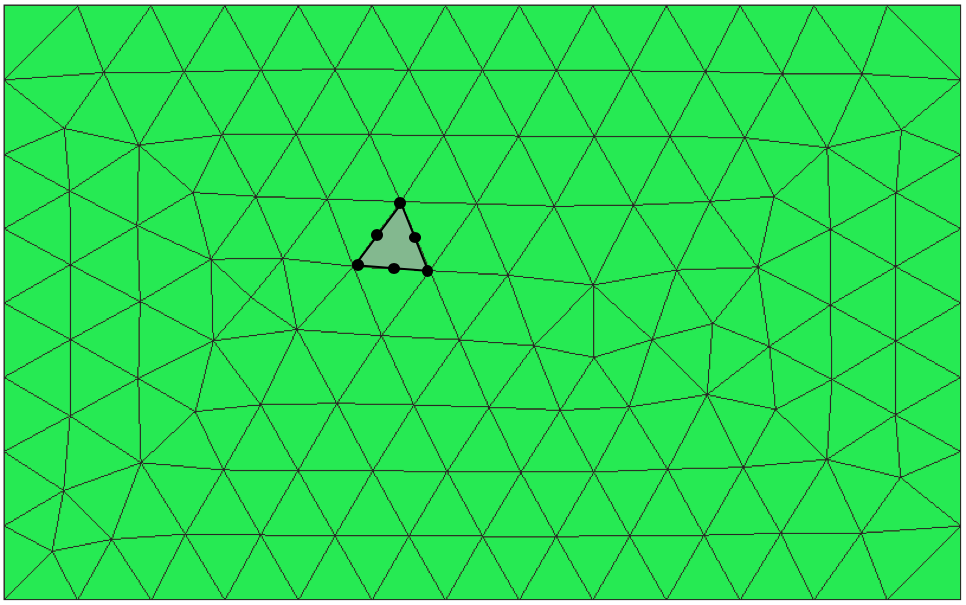
\includegraphics[width=0.45\linewidth]{figs/fe_mesh.png}
\caption{Illustration of a continuous domain discretized into triangular finite elements.}
\label{fig:fe_mesh}
\end{figure}

If \(\psi\) and \(\phi\) are nonzero over the entire domain, every region of the problem is tightly coupled to all other regions, resulting in a dense matrix system. A sparse system can be attained by restricting the shape functions to a nodal basis such that

\beq
\label{eq:Nodal}
\phi_i(\Omega_j)=\delta_{ij}\ ,
\eeq

\noindent where \(\Omega_j\) is the coordinate describing the location of the \(j\)-th node and \(\delta_{ij}\) is the Kronecker delta. The number of nodes in the entire domain, \(N\), determines the number of basis functions used in the approximate solution in Eq.\ \eqref{eq:WRExpansion}. Unless otherwise noted, first-order Lagrange basis functions are used for all solution variables in this work, though the \gls{moose} framework supports higher orders and many other shape function families, such as Hermite and monomial functions.

The boundary terms in Eqs.\ \eqref{eq:PronghornEquations_V2WeakForm}--\eqref{eq:MultiscaleWeak} are integrals over the entire boundary. The boundary may in general be decomposed into the portion on which Dirichelt conditions are specified, \(\Gamma_\text{Dirichlet}\), and the portion on which Neumann conditions are specified, \(\Gamma_\text{Neumann}\). The boundary is the union of these two boundaries

\beq
\Gamma\equiv\Gamma_\text{Dirichlet}\cup\Gamma_\text{Neumann}\ ,
\eeq

\noindent where \(\Gamma_\text{Dirichlet}\cap\Gamma_\text{Neumann}=\emptyset\). On Dirichlet boundaries, the fluxes appearing in the boundary integrals may be unknown. Rather than back-calculating the flux that results in the desired Dirichlet condition on the primal variable, Dirichlet conditions are imposed by requiring

\beq
\psi=0\text{ for }\Gamma\in\Gamma_\text{Dirichlet}\ .
\eeq

\noindent All Dirichlet \glspl{bc} in Pronghorn are strongly enforced. The \texttt{DirichletBC} class, a child of the \texttt{BoundaryCondition} class, abstracts the implementation details of the ``removal'' of Dirichlet nodes from the solve.

\subsection{Method of Lines Time Stepping}
\label{sec:mol}

The expansion used for the approximate solution in Eq.\ \eqref{eq:WRExpansion} is assumed separable in space and time. That is, the expansion coefficients \(C\) are only functions of time, while the basis functions \(\phi\) are only functions of space. All time derivatives in Eqs.\ \eqref{eq:PronghornEquations_V2WeakForm}--\eqref{eq:MultiscaleWeak} are replaced by \gls{fd} approximations, a method that is often referred to as the \gls{mol}. For time step \(n+1\), all other terms in the weak form are evaluated at time \(m\) or time \(m+1\) for explicit and implicit \gls{fd} approximations, respectively.

The \gls{moose} framework abstracts much of the details of the \gls{mol} implementation to \gls{moose} framework classes and the \gls{petsc} library. For instance, there is no time indexing in the variables and material properties referenced in the example source snippets shown in Listings \ref{lst:one} and \ref{lst:two}. Application developers take advantage of polymorphism to represent time derivatives in the source implementation agnostic of the discretization, similar to the spatial representation shown in Section \ref{sec:weak_form}. For example, the source code responsible for residual calculation of the time derivative contribution to Eqs.\ \eqref{eq:MassWeak} and \eqref{eq:Mass2Weak} at a quadrature point is shown in Listing \ref{lst:three}.

\vspace{1em}
\begin{minipage}[c]{0.92\linewidth}
\begin{lstlisting}[caption={Pronghorn source code calculation of \(\int_\Omega\epsilon\frac{\partial\rho_f}{\partial t}\psi d\Omega\).},captionpos=b,label={lst:three}]
Real
MassTimeDerivative::computeQpResidual()
{
  return _epsilon[_qp] * _drho_f_dt[_qp] * _test[_i][_qp];
}
\end{lstlisting}
\end{minipage}

\texttt{MassTimeDerivative} is the kernel class name, \texttt{\_drho\_f\_dt} is the name of the density time derivative \(\partial\rho_f/\partial t\) material coupled to the kernel, and \texttt{\_test} is the name of the weight function \(\psi\). Other terms have the same interpretation as in Listings \ref{lst:one} and \ref{lst:two}. Unless otherwise noted, an implicit Euler discretization is used for all time derivatives in this work.

\subsection[Streamline Upwind Petrov-Galerkin Stabilization]{SUPG Stabilization}
\label{sec:supg}

The continuous \gls{fem} is well-known to be conditionally stable for convection-diffusion equations. Consider the \gls{1d}, linear convection-diffusion equation,

\beq
\label{eq:1DConvectionDiffusion}
-\alpha_d\frac{\partial^2\upsilon}{\partial x^2}+V\frac{\partial \upsilon}{\partial x}=0\ ,
\eeq

\noindent where \(\alpha_d\) is the diffusivity, \(V\) is the velocity, and \(\upsilon\) is a transported scalar. For a linear Lagrange interpolation on uniform elements, the stability criterion for Eq.\ \eqref{eq:1DConvectionDiffusion} is straightforward to derive and is shown in ref. \cite{novak_manual}. This derivation yields

\beq
\label{eq:PeCriterion}
Pe_{el}>1\ ,
\eeq

\noindent where \(Pe_{el}\) is the element Peclet number, defined as

\beq
\label{eq:PeEl}
Pe_{el}\equiv\frac{\|\vec{V}\|h_e}{2\alpha_d}\ ,
\eeq

\noindent where \(h_e\) is the element size. For generality, Eq.\ \eqref{eq:PeEl} is shown in terms of a general diffusivity \(\alpha_d\) rather than the thermal diffusivity \(k/\rho C_p\) used in the definition of \(Pe\) in Eq.\ \eqref{eq:PecletDef}. 

It can be shown that a linear Lagrange interpolation of Eq.\ \eqref{eq:1DConvectionDiffusion} on uniform elements is equivalent to a central \gls{fd} approximation of both the diffusive and convective kernels. This symmetric discretization results in non-physical nodal oscillations for flows with \(Pe_{el}>1\) with magnitudes that tend to increase with \(Pe_{el}\) \cite{novak_manual,zienkiewicz}. 

Fig.\ \ref{fig:Convection_vs_Diffusion} illustrates typical convective and diffusive processes transporting a passive scalar in both space and time between the same \gls{ic} and the same end time. While diffusion is a symmetric phenomenon, convection transports in the direction of velocity such that the flow at a point is only dependent on the upstream conditions. This observation is the underlying cause of the numeric instability\mdash a symmetric discretization of the convective derivative is a poor representation of convective physics unless the symmetry of the diffusive process dominates the upwind nature of convection, or \(Pe_{el}<1\). The same conclusion can be shown in more rigorous manner in terms of the self-adjoint and non-self-adjoint properties of diffusion and convection operators, respectively \cite{zienkiewicz}.

\begin{figure}[!h]
\centering
\begin{subfigure}{.45\textwidth}
  \centering
  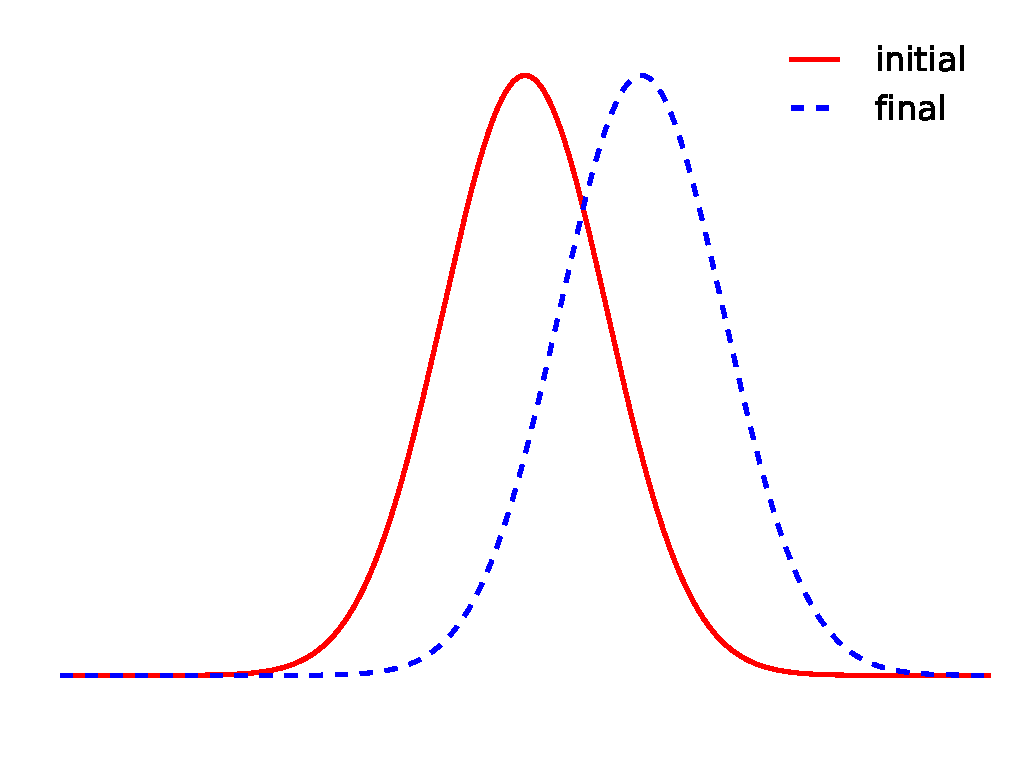
\includegraphics[width=0.9\linewidth]{figs/convective_process.pdf}
  \caption{Convective phenomenon}
\end{subfigure}
\begin{subfigure}{.45\textwidth}
  \centering
  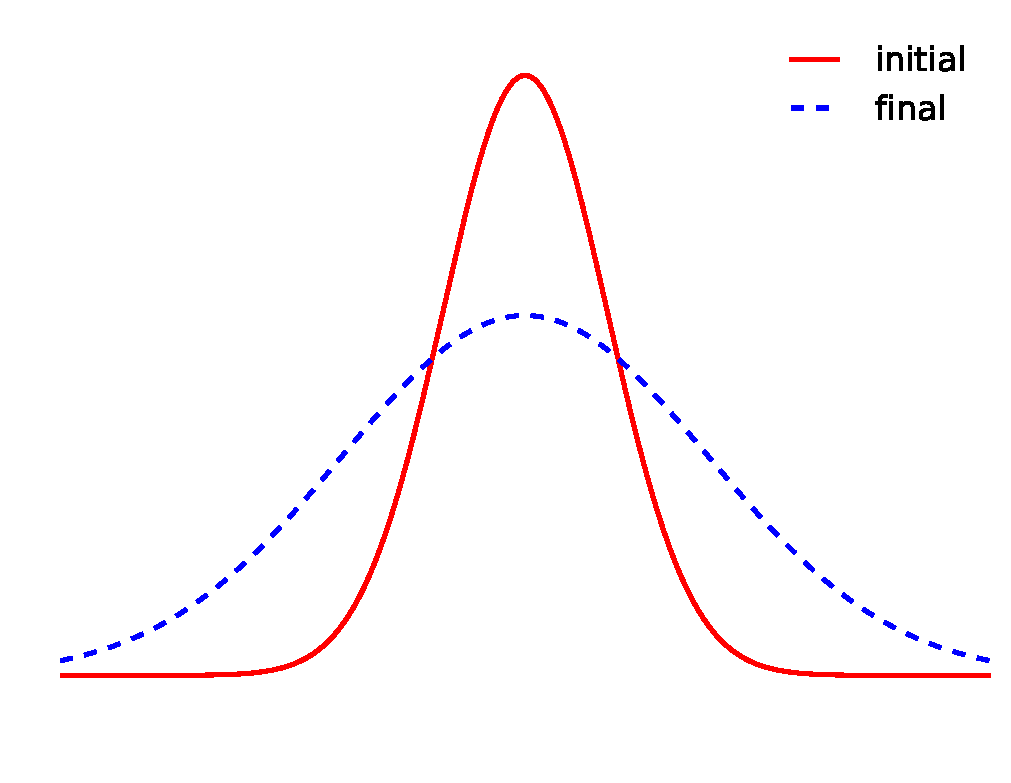
\includegraphics[width=0.9\linewidth]{figs/diffusive_process.pdf}
  \caption{Diffusive phenomenon}
\end{subfigure}
\caption{Difference between (a) convective (flow from left to right) and (b) diffusive transport of a passive scalar from the same \gls{ic} (---) to the same end time (- - -).}
\label{fig:Convection_vs_Diffusion}
\end{figure}

For systems with some diffusion, the mesh can in theory be refined until \(Pe_{el}<1\); however, this strategy is often prohibitively expensive. This section describes an upwind Petrov-Galerkin method that supplements the weak forms in the fluid conservation equations with additional integrals that act to discretize the convective kernels with upwind approximations to better match the directional dependence of convection.

Petrov-Galerkin methods differ from Bubnov-Galerkin methods in that the approximate solution and the weight function no longer live in the same function space; that is, \(\psi\) is no longer given by Eq.\ \eqref{eq:PsiExpansion}. For the Petrov-Galerkin methods considered here, the weight function is instead given as the sum of the original element-continuous weight functions \(\psi\) and an element-discontinuous function \(\psi^\star\),

\beq
\label{eq:pgwf}
\tilde{\psi}=\psi+\psi^\star\ ,
\eeq

\noindent where \(\tilde{\psi}\) represents the Petrov-Galerkin weight function and \(\psi\) is given by Eq.\ \eqref{eq:PsiExpansion}. The weighted residual statement in Eq.\ \eqref{eq:GalerkinInt3} becomes

\beq
\label{eq:PG}
\int_{\Omega}\left\lbrack R\left(C_j\phi_j\right)\right\rbrack^*\phi_i\ d\Omega+\int_{\Omega}\left\lbrack R\left(C_j\phi_j\right)\right\rbrack^*\psi^\star_i\ d\Omega=0\hspace{1cm}\text{for }j\in N\ .
\eeq

\noindent The first integral is the same Bubnov-Galerkin weighted residual statement from Eq.\ \eqref{eq:GalerkinInt3}. While the first integral in Eq.\ \eqref{eq:PG} is integrated by parts where possible, the second integral cannot be integrated by parts because \(\psi^\star\) is discontinuous across elements. If the approximate solution shape functions are sufficiently differentiable to have nonzero and finite derivatives in the second term, the Petrov-Galerkin method is consistent\mdash that is, the solution to Eq.\ \eqref{eq:PG} is the same as the solution to the Bubnov-Galerkin form in Eq.\ \eqref{eq:GalerkinInt3}.

For a linear Lagrange interpolation of Eq.\ \eqref{eq:1DConvectionDiffusion} on uniform elements, selecting \(\psi^\star\) as

\beq
\label{eq:psiStar}
\psi^\star=\frac{h_e}{2\|\vec{V}\|}\vec{V}\cdot\nabla\psi\ 
\eeq

\noindent is equivalent to a central \gls{fd} approximation of the diffusive kernel and an upwind approximation of the convective kernel that eliminates the \(Pe_{el}\) stability criterion \cite{zienkiewicz,brooks,novak_manual}. 

In 1981, Brooks developed a consistent generalization of Eq.\ \eqref{eq:psiStar} to multi-dimensional, coupled, systems of convection-diffusion equations known as the \gls{supg} method that is now widely used in continuous \gls{fem} discretizations of convection-diffusion systems \cite{hauke,tezduyar,kirk,hauke_1998,TH1983,tezduyar1983,zienkiewicz,StabilizationReview}. The remainder of this section describes the application of the \gls{supg} stabilization scheme to the macroscale equations described in Chapter \ref{sec:PhysicalModels}. A detailed discussion of the stabilization is presented to illustrate the extension of the original \gls{supg} method to porous flows. 

The Navier-Stokes and friction-dominated fluid conservation equations are sufficiently different to warrant separate discussions of the \gls{supg} stabilization for each model. Stabilization of the Navier-Stokes model is described first due to its similarity to the conservative forms of convection-diffusion equations for which the \gls{supg} method was originally formulated. Rewrite the fluid conservation equations in the Navier-Stokes model in Eq.\ \eqref{eq:PorousEquations} in compact notation as

\beq
\label{eq:NSConcise}
\frac{\partial(\epsilon\vec{U})}{\partial t}+\frac{\partial(\epsilon\vec{F}_i)}{\partial x_i}-\frac{\partial\vec{G}_i}{\partial x_i}+\vec{S}=\vec{0}\ ,
\eeq

\noindent where \(\vec{U}\) is the vector of conserved quantities,

\beq
\label{eq:EulerNL}
\vec{U}\equiv\begin{bmatrix}\rho_f\\\rho_f V_1\\\rho_f V_2\\\rho_f V_3\\\rho_f E_f
\end{bmatrix}\ ;
\eeq

\noindent \(\vec{F}_i\) is the inviscid flux vector in the \(i\)-th dimension,

\beq
\label{eq:EulerIF}
\vec{F}_i\equiv \begin{bmatrix}\rho_fV_i \\ \rho_f V_1V_i+ P\delta_{1i}\\\rho_f V_2V_i+ P\delta_{2i}\\\rho_f V_3V_i+ P\delta_{3i}\\ \rho_f V_iH_f
\end{bmatrix}\ ;
\eeq

\noindent \(\vec{G}_i\) is the diffusive flux vector in the \(i\)-th dimension,

\beq
\label{eq:PHEquationsConcise}
\vec{G}_i\equiv\begin{bmatrix}0\\\tilde{\mu}\frac{\partial V_1}{\partial x_i}\\\tilde{\mu}\frac{\partial V_2}{\partial x_i}\\\tilde{\mu}\frac{\partial V_3}{\partial x_i}\\ \kappa_f\frac{\partial T_f}{\partial x_i}
\end{bmatrix}\ ;
\eeq

\noindent and \(\vec{S}\) is the source vector,

\beq
\label{eq:EulerS}
\vec{S}=\begin{bmatrix}0\\-\epsilon\rho_fg_1+W\rho_fV_1+P\frac{\partial\epsilon}{\partial x_1}\\-\epsilon\rho_fg_2+W\rho_fV_2+P\frac{\partial\epsilon}{\partial x_2}\\-\epsilon\rho_fg_3+W\rho_fV_3+P\frac{\partial\epsilon}{\partial x_3}\\ -\epsilon\rho_fg_iV_i+\alpha(T_f-T_s)-\dot{q}_f
\end{bmatrix}\ .
\eeq

\noindent For notational simplicity, \(\epsilon\) is shown within the time differentiation term in Eq.\ \eqref{eq:NSConcise} though the actual implementation assumes porosity is independent of time. Define a quasi-linear residual \(\vec{\mathscr{R}}\) as

\beq
\label{eq:StrongResidual}
\vec{\mathscr{R}}\equiv\frac{\partial(\epsilon\vec{U})}{\partial t}+\epsilon\textbf{A}_i\frac{\partial\vec{U}}{\partial x_i}+\vec{F}_i\frac{\partial\epsilon}{\partial x_i}-\frac{\partial \vec{G}_i}{\partial x_i}+\vec{S}\ ,
\eeq

\noindent where \(\textbf{A}_i\) are the inviscid flux Jacobian matrices,

\beq
\label{eq:IFJM}
\textbf{A}_i\equiv\frac{\partial\vec{F}_i}{\partial\vec{U}}\ .
\eeq

\noindent The inviscid flux Jacobian matrices require the partial derivatives of \(P\), \(H_f\), and the components of \(\vec{U}\) with respect to the components of \(\vec{U}\). The partial derivative of \(U_i\) with respect to \(U_j\) is

\beq
\label{eq:UDerivs}
\frac{\partial U_i}{\partial U_j}=\delta_{ij}\ ,
\eeq

\noindent The derivative of \(H_f\) with respect to \(\vec{U}\) is

\beq
\frac{\partial H_f}{\partial \vec{U}}=\frac{1}{\rho_f}\begin{bmatrix}\frac{\partial P}{\partial U_0}-H_f & \frac{\partial P}{\partial U_1} & \frac{\partial P}{\partial U_2} & \frac{\partial P}{\partial U_3} & \frac{\partial P}{\partial U_4}+1\end{bmatrix}\ .
\eeq

\noindent The derivative of pressure with respect to \(\vec{U}\) is written in the form of a chain rule as

\beq
\label{eq:PressureDerivsCons}
\frac{\partial P}{\partial \vec{U}}=\frac{\partial P}{\partial v_f}\frac{\partial v_f}{\partial \vec{U}}+\frac{\partial P}{\partial e_f}\frac{\partial e_f}{\partial \vec{U}}\ ,
\eeq

\noindent where \(v_f\) is the fluid intrinsic phase averaged specific volume; \(\partial P/\partial v_f\) and \(\partial P/\partial e_f\) are obtained from the \gls{eos}; \(\partial v_f/\partial \vec{U}\) is given as

\beq
\label{eq:dvdU}
\frac{\partial v_f}{\partial \vec{U}}=\begin{bmatrix}\frac{1}{\rho_f^2} & 0 & 0 & 0 & 0\end{bmatrix}\ ;
\eeq

\noindent and \(\partial e_f/\partial \vec{U}\) is given as

\beq
\label{eq:dedU}
\frac{\partial e_f}{\partial \vec{U}}=\frac{1}{\rho_f}\begin{bmatrix}\|\vec{V}\|^2-E_f & -V_1 & -V_2 & -V_3 & 1\end{bmatrix}\ .
\eeq

\noindent With the derivatives in Eqs.\ \eqref{eq:UDerivs}--\eqref{eq:dedU}, the inviscid flux Jacobian matrices are

\beq
\label{eq:IFJMi}
\textbf{A}_i=
\begin{bmatrix}
0 & \delta_{1i} & \delta_{2i} & \delta_{3i} & 0\\
\frac{-U_1U_i}{U_0^2}+\delta_{1i}\frac{\partial P}{\partial U_0} & \delta_{1i}\zeta_1+\tilde{\delta}_{1i}\frac{U_i}{U_0} & \delta_{i2}\frac{U_1}{U_0}+\delta_{1i}\frac{\partial P}{\partial U_2} & \delta_{i3}\frac{U_1}{U_0}+\delta_{1i}\frac{\partial P}{\partial U_3} & \delta_{1i}\frac{\partial P}{\partial U_4}\\
\frac{-U_2U_i}{U_0^2}+\delta_{2i}\frac{\partial P}{\partial U_0} & \delta_{1i}\frac{U_2}{U_0}+\delta_{2i}\frac{\partial P}{\partial U_1} & \delta_{2i}\zeta_2+\tilde{\delta}_{2i}\frac{U_i}{U_0} & \delta_{i3}\frac{U_2}{U_0}+\delta_{2i}\frac{\partial P}{\partial U_3} & \delta_{2i}\frac{\partial P}{\partial U_4}\\
\frac{-U_3U_i}{U_0^2}+\delta_{3i}\frac{\partial P}{\partial U_0} & \delta_{1i}\frac{U_3}{U_0}+\delta_{3i}\frac{\partial P}{\partial U_1} & \delta_{2i}\frac{U_3}{U_0}+\delta_{3i}\frac{\partial P}{\partial U_2} & \delta_{3i}\zeta_3+\tilde{\delta}_{3i}\frac{U_i}{U_0} & \delta_{3i}\frac{\partial P}{\partial U_4}\\
U_i\frac{\partial H_f}{\partial U_0} & U_i\frac{\partial H_f}{\partial U_1}+\delta_{1i}H_f & U_i\frac{\partial H_f}{\partial U_2}+\delta_{2i}H_f & U_i\frac{\partial H_f}{\partial U_3}+\delta_{3i}H_f & U_i\frac{\partial H_f}{\partial U_4}\\
\end{bmatrix}\ ,
\eeq

\noindent where the following terms are defined for conciseness,

\beq
\label{eq:tilde_delta}
\tilde{\delta}_{ij}\equiv1-\delta_{ij}\ ,
\eeq

\beq
\label{eq:zeta_placeholder}
\zeta_i\equiv\frac{2U_i}{U_0}+\frac{\partial P}{\partial U_i}\ .
\eeq

\noindent All prerequisite notation has been introduced to now describe the stabilization. The \gls{supg} method adds the following integral to the Bubnov-Galerkin weak form,

\beq
\label{eq:supg1}
\int_\Omega\epsilon\left\lbrack\textbf{A}_i\left(\tau_{SUPG}\ \vec{\mathscr{R}}\right)\right\rbrack\cdot\frac{\partial\vec{W}}{\partial x_i}d\Omega\ ,
\eeq

\noindent where \(\tau_{SUPG}\) is a matrix of stabilization coefficients and \(\vec{W}\) is the vector of weight functions corresponding to each coupled equation. To clearly illustrate the indexing, rewrite Eq.\ \eqref{eq:supg1} as

\beq
\label{eq:supg2}
\int_\Omega\epsilon\textbf{A}_{i,jk\ }\tau_{SUPG,kl\ }\mathscr{R}_l\frac{\partial W_j}{\partial x_i}d\Omega\ .
\eeq

\noindent For the five coupled equations in Eq.\ \eqref{eq:NSConcise} in three spatial dimensions, \(j\), \(k\), \(l=1,2,3,4,5\) and \(i=1,2,3\). In other words, \(j\), \(k\), \(l\) represent the number of coupled equations and \(i\) represents the number of spatial dimensions. The weak form of the Navier-Stokes model with the \gls{supg} stabilization is then

\beqa
\label{eq:EqnWeakForm}
\int_{\Omega}\left\lbrack\epsilon\vec{W}\cdot\frac{\partial\vec{U}}{\partial t}+\frac{\partial\vec{W}}{\partial x_i}\cdot\left(\vec{G}_i-\epsilon\vec{F}_i\right)+\vec{W}\cdot\vec{S}\right\rbrack d\Omega+\int_{\Gamma}\left(\epsilon\vec{F}_i-\vec{G}_i\right)\cdot\vec{W}n_id\Gamma\ +\hspace{1cm}\\
\int_\Omega\epsilon\left\lbrack\textbf{A}_i\left(\tau_{SUPG}\ \vec{\mathscr{R}}\right)\right\rbrack\cdot\frac{\partial\vec{W}}{\partial x_i}d\Omega=0\ ,
\eeqa

\noindent where integration by parts is applied only to the element-continuous terms. The first two integrals in Eq.\ \eqref{eq:EqnWeakForm} have already been presented in Eq.\ \eqref{eq:PronghornEquations_V2WeakForm}.

While perhaps not immediately apparent, Eq.\ \eqref{eq:supg1} is equivalent to upwinding in directions parallel to the velocity vector. To the \(j\)-th coupled equation is added an integral involving terms proportional to \(\vec{V}\cdot\nabla W_j\), \(\vec{\mathscr{R}}_u\cdot\nabla W_j\), and \(\partial W_j/\partial x_j\) (no summation implied), where \(\vec{\mathscr{R}}_u\) is the vector of momentum quasi-linear strong residuals. These new terms have a clear resemblance to the \gls{1d} \(\psi^\star\) in Eq.\ \eqref{eq:psiStar} that introduced an upwind discretization of the convective derivative, but now generalized to coupled systems of equations. As an instructive example, Appendix \ref{sec:supg_app} shows the \gls{supg} integrals in Eq.\ \eqref{eq:EqnWeakForm} for the mass, momentum, and energy conservation equations in the Navier-Stokes model with the ideal gas \gls{eos}.

The friction-dominated model lacks convective terms in the momentum conservation equations and the fluid energy conservation equation is not written in conservative form. Rather than cast the friction-dominated model into the notation in Eq.\ \eqref{eq:NSConcise}, carrying through the algebra in Eq.\ \eqref{eq:supg1} shows that a term proportional to \(\vec{\mathscr{R}}_i\cdot\nabla W_0\) is added to the Navier-Stokes mass conservation equation. Extending this concept to the friction-dominated model, the following integral is added to the friction-dominated mass conservation equation,

\beq
\label{eq:fd1}
\int_\Omega \tilde{\tau}\left(\epsilon\nabla P-\epsilon\rho_f\vec{g}+W\rho_f\vec{V}\right)\cdot\nabla\psi d\Omega\ ,
\eeq

\noindent where \(\tilde{\tau}\) is a scalar stabilization parameter. The weak form of the friction-dominated mass conservation equation with the \gls{supg} stabilization is then

\beqa
\label{eq:qqq1}
\int_\Omega\epsilon\frac{\partial\rho_f}{\partial t}\psi d\Omega-\int_\Omega\left\lbrack\frac{\epsilon^2}{W}\left(\rho_f\vec{g}-\nabla P\right)\right\rbrack\cdot\nabla\psi d\Omega+\int_\Gamma\left\lbrack\frac{\epsilon^2}{W}\left(\rho_f\vec{g}-\nabla P\right)\right\rbrack \psi d\Gamma+\hspace{1cm}\\
\int_\Omega \tilde{\tau}\left(\epsilon\nabla P-\epsilon\rho_f\vec{g}+W\rho_f\vec{V}\right)\cdot\nabla\psi d\Omega=0\ .
\eeqa

\noindent The first two integrals in Eq.\ \eqref{eq:qqq1} have already been presented in Eq.\ \eqref{eq:Mass2Weak}. No additional integrals are added to the momentum conservation equations due to the lack of convective terms. 

Finally, the fluid energy conservation equation is stabilized using the single-equation form suggested by Eq.\ \eqref{eq:psiStar} by adding the following integral to the fluid energy conservation equation,

\beq
\label{eq:fd2}
\int_\Omega\tilde{\tau}\left\lbrack\epsilon\rho_fC_{p,f}\frac{\partial T_f}{\partial t}+\epsilon\rho_fC_{p,f}\vec{V}\cdot\nabla T_f-\nabla\cdot(\kappa_f\nabla T_f)+\alpha(T_f-T_s)-\dot{q}_f\right\rbrack\vec{V}\cdot\nabla \psi d\Omega\ .
\eeq

\noindent The weak form of the friction-dominated fluid energy conservation equation with the \gls{supg} stabilization is then

\beqa
\label{eq:qqq2}
\int_\Omega\left\lbrack\epsilon\rho_fC_{p,f}\frac{\partial T_f}{\partial t}+\epsilon\rho_fC_{p,f}\vec{V}\cdot\nabla T_f+\alpha(T_f-T_s)-\dot{q}_f\right\rbrack\psi d\Omega+\int_\Omega\kappa_f\nabla T_f\cdot\nabla \psi d\Omega\ +\hspace{0.3cm}\\
\int_\Gamma\kappa_f\nabla T_f\cdot\hat{n}\psi d\Gamma+\int_\Omega\tilde{\tau}\left(\epsilon\rho_fC_{p,f}\frac{\partial T_f}{\partial t}+\epsilon\rho_fC_{p,f}\vec{V}\cdot\nabla T_f\right)\vec{V}\cdot\nabla\psi d\Omega\ +\hspace{0.15cm}\\
\int_\Omega\tilde{\tau}\left\lbrack-\nabla\cdot(\kappa_f\nabla T_f)+\alpha(T_f-T_s)-\dot{q}_f\right\rbrack\vec{V}\cdot\nabla \psi d\Omega=0\ .
\eeqa

\noindent The first two integrals in Eq.\ \eqref{eq:qqq2} have already been presented in Eq.\ \eqref{eq:Energy2Weak}. The \gls{supg} stabilization terms in Eq.\ \eqref{eq:supg1} for the Navier-Stokes model and Eqs.\ \eqref{eq:fd1} and \eqref{eq:fd2} for the friction-dominated model are implemented in Pronghorn in a similar manner as the other kernels as described in Section \ref{sec:weak_form}. 

\(\tau_{SUPG}\) represents a matrix of intrinsic time scales; for coupled systems of equations, each component in \(\tau_{SUPG}\) is a combination of the waves associated with the eigenvalues of the equation system. Rather than solve an eigenvalue problem at each quadrature point, computational efficiency motivates a diagonal approximation,

\beq
\label{eq:tauSUPG}
\tau_{SUPG}=\begin{bmatrix}
\tau_c & 0 & 0 & 0 & 0\\
0 & \tau_{u} & 0 & 0 & 0\\
0 & 0 & \tau_{u} & 0 & 0\\
0 & 0 & 0 & \tau_{u} & 0\\
0 & 0 & 0 & 0 & \tau_e\\
\end{bmatrix}\ ,
\eeq

\noindent where the stabilization parameters for the mass, momentum, and energy conservation equations are \(\tau_c\), \(\tau_u\), and \(\tau_e\), respectively \cite{hauke,tezduyar,hauke_1998,kirk,TH1983,tezduyar1983}. \(\tau_c\), \(\tau_u\), and \(\tau_e\) are typically selected as characteristic time scales representing normalized temporal, advective, and diffusive terms in the weak form \cite{tezduyar}. 

Three different time scales are considered in the construction of \(\tau_c\), \(\tau_u\), and \(\tau_e\)\mdash 1)~a transient limit, \(\tau_\text{temporal}\); 2)~an advective limit, \(\tau_\text{advective}\); and 3)~a diffusive limit, \(\tau_\text{diffusive}\). These time scales are combined into a single representative time scale with smooth transitions among its components,

\beq
\label{eq:switchTau}
\tau_j=\left\lbrack\left(\frac{1}{\tau_\text{temporal}}\right)^2+\left(\frac{1}{\tau_\text{advective}}\right)^2+\left(\frac{1}{\tau_\text{diffusive}}\right)^2\right\rbrack^{-1/2}\ ,
\eeq

\noindent where \(j=c\), \(u\), \(e\). The \(\tau_\text{temporal}\), \(\tau_\text{advective}\), and \(\tau_\text{diffusive}\) terms may in general be unique for each of the conservation equations. However, for the present analysis, the mass, momentum, and energy conservation equations share the same advective and temporal limits. The advective limit is given as

\beq
\label{eq:tau1}
\tau_\text{advective}=\frac{h_e}{2\left(\|\vec{V}\|+c\right)}\ ,
\eeq

\noindent and the temporal limit is given as

\beq
\label{eq:tau2}
\tau_\text{temporal}=\frac{\Delta t}{2}\ .
\eeq

\noindent Lacking diffusive terms, there is no diffusive limit for the mass conservation equation. For the momentum conservation equation, the diffusive limit is given as

\beq
\label{eq:tau3}
\tau_\text{diffusive}=\frac{\rho_fh_e^2}{4\left(\tilde{\mu}/\epsilon\right)}\ ,
\eeq

\noindent while for the energy conservation equation is given as

\beq
\label{eq:tau4}
\tau_\text{diffusive}=\frac{\rho_fC_{p,f}h_e^2}{4\left(\kappa_f/\epsilon\right)}\ .
\eeq

\noindent The scalar stabilization parameter \(\tilde{\tau}\) in the \gls{supg} stabilization of the friction-dominated model is taken as Eq.\ \eqref{eq:tau4}. The element size \(h_e\) is for simplicity taken as the minimum dimension of the element, though methods based on flow-aligned or element-averaged scales have been used elsewhere \cite{hauke_1998,hauke,tezduyar1983,tezduyar}. 

The selection of \(\tau_{SUPG}\) requires a balance between accuracy and stability\mdash too small a \(\tau_{SUPG}\) will still exhibit nodal oscillations, while too large a \(\tau_{SUPG}\) will result in excessive diffusion for basis functions with orders less than the highest derivative in the strong form \gls{pde}. The above definitions for \(\tau_c\), \(\tau_u\), and \(\tau_e\) are only approximate, and a multiplier \(\tilde{C}\) is used to scale the stabilization parameter. All simulations should be run for a number of \(\tilde{C}\) values to determine an appropriate balance between stability and accuracy. \

\section{Solution Methods}
\label{sec:solution}
This section describes the numerical solution of the coupled system of macroscale, mesoscale, and microscale equations. A Picard iteration described in Section \ref{sec:multiscale_solution} is used to couple the solutions on the three length scales, where the solution on each individual scale is obtained with a Newton-Krylov method described in Section \ref{sec:nonlinear}.

\subsection{Picard Iteration of Multiple Applications}
\label{sec:multiscale_solution}

Coupling between the macro, meso, and micro length scales is achieved using Picard iteration. The \gls{moose} framework uses a hierarchical tree-like system to control execution of and data transfer between multiple applications within a single simulation. A ``master'' application controls a number of sub-applications and facilitates data transfer between itself and the sub-applications. Each sub-application may itself control a number of sub-applications, locally acting as a master application to sub-applications double nested relative to the top-level application. 

The coupling tree is highly parallelized. The master application uses all processors, while all its sub-applications run simultaneously in parallel with the resources allocated to the local master application. For instance, consider a three-tiered coupling system with application \(\mathcal{A}\) controlling five sub-applications \(\mathcal{B}_i\) for \(i=1\cdots 5\), each of which controls two sub-applications \(\mathcal{C}_{ij}\) for \(j=1, 2\). Allocating a total of 60 \gls{mpi} processes to application \(\mathcal{A}\) will run each of the \(\mathcal{B}\) applications with 12 processes and each of the \(\mathcal{C}\) applications with 6 processes; all \(\mathcal{B}\) processes run in parallel with one another and all \(\mathcal{C}\) processes run in parallel with one another. 

\gls{moose}'s coupling system specifically aims to address many of the shortcomings of earlier multiphysics simulations that relied on rigid one-to-one spatial and temporal data transfers through the file system. All \gls{moose} applications may be coupled on different spatial meshes with subcycling time stepping, and all data is communicated in memory. 
% TODO - could cite multiphysics papers here

As an example, Fig.\ \ref{fig:multiapp} illustrates one possible execution and communication structure within a single Picard iteration for a simulation involving two applications on the same spatial domain. Both the master application and sub-application may in general solve a set of coupled nonlinear equations. In Picard iteration \(n\) within the time step incrementing to simulation time \(t\), the master application first solves a set of coupled equations with the Newton-Krylov method described in Section \ref{sec:nonlinear}. The master application then transfers the variable \(T\) to a sub-application that depends on that variable, such as through a source term or material property. Interpolation between meshes, sampling from element centroids, and functional expansions are several of the mechanisms available for representing data transfers between applications. For this example, Fig.\ \ref{fig:multiapp} depicts this data transfer as a mesh interpolation. Next, the sub-application solves a set of coupled equations with the Newton-Krylov method described in Section \ref{sec:nonlinear}. The master application then retrieves the variable \(\phi\) from the sub-application to use in dependent terms in its set of equations. The coupled simulation is converged and proceeds to the next time step if the relative change in the solution from the previous Picard iteration is less than a specified tolerance. If not converged, the Picard iteration is repeated. The example illustrated in Fig.\ \ref{fig:multiapp} is fairly simplistic, and the multi-application execution and data transfer system in \gls{moose} accommodates many other types of coupling, such as scalar and boundary coupling, with more fine-grained communication patterns. 

\begin{figure}[!h]
\centering
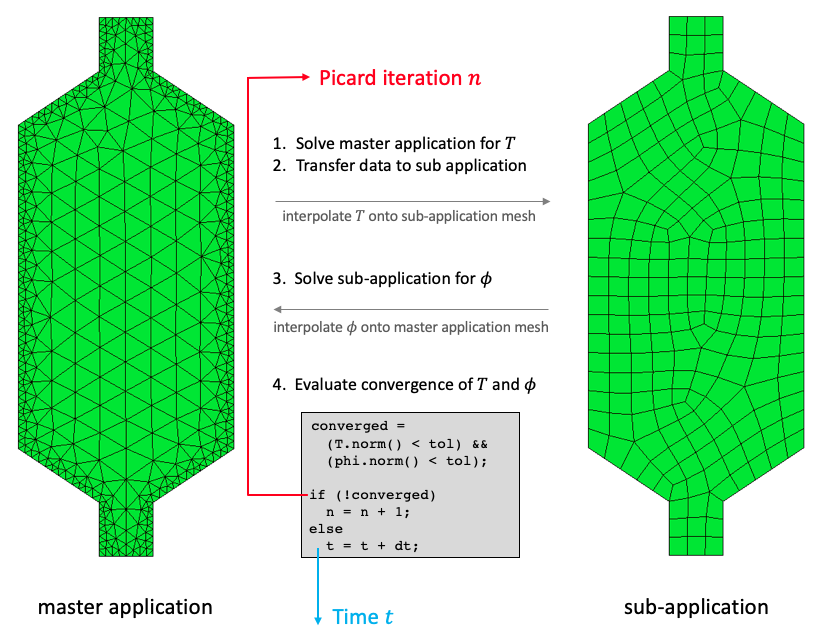
\includegraphics[width=0.9\linewidth]{figs/multiapp.png}
\caption{Illustration of one possible execution and communication structure for coupling multiple applications within the \gls{moose} framework.}
\label{fig:multiapp}
\end{figure}

Fig.\ \ref{fig:multiscale_pbr} shows an illustration of the length scale coupling in Pronghorn when the \gls{hsd} is used to describe the internal pebble heat transfer. The macroscale model is the master application, which controls the execution of the ``first-tier'' mesoscale sub-applications. Each mesoscale application controls the execution of the ``second-tier'' microscale sub-applications. In a single Picard iteration, the multiscale coupling procedure with the \gls{hsd} meso and micro scale model is as follows\mdash

\begin{enumerate}
\itemsep0.3em
\item The master application solves the macroscale model.
\item The master application calculates the average solid surface temperature \(T_s\) and solid power density in each element of the macroscale mesh.
\item The master application transfers the averaged solid surface temperature as a \gls{bc} and the averaged solid power density as a source term to a mesoscale sub-application in each element. Six macroscale elements are highlighted in Fig.\ \ref{fig:multiscale_pbr}; the ``color'' in the element represents the magnitude of the solid surface temperature used as a \gls{bc} in the mesoscale model. Note the similarity of this process to that illustrated in Fig.\ \ref{fig:meso}.
\item The first-tier sub-applications solve the mesoscale models, which themselves consist of several steps repeated until convergence of the pebble temperature distribution\mdash
	\begin{enumerate}
  \itemsep0.3em
	\item The first-tier sub-applications solve the mesoscale model given a previous microscale solution in each element of the mesoscale mesh.
	\item The first-tier sub-applications calculate averaged power densities in each element of the mesoscale mesh.
	\item The first-tier sub-applications transfer the averaged power densities as a source term to a microscale sub-application in each element.
	\item The second-tier sub-applications solve the microscale models.
	\item The first-tier sub-applications retrieve the microscale solution in each element of the mesoscale mesh and apply the continuity in heat flux and temperature \gls{bc} with the summation in Eq.\ \eqref{eq:MultiscaleSolution}.
	\end{enumerate}
\end{enumerate}

\begin{figure}[!h]
\centering
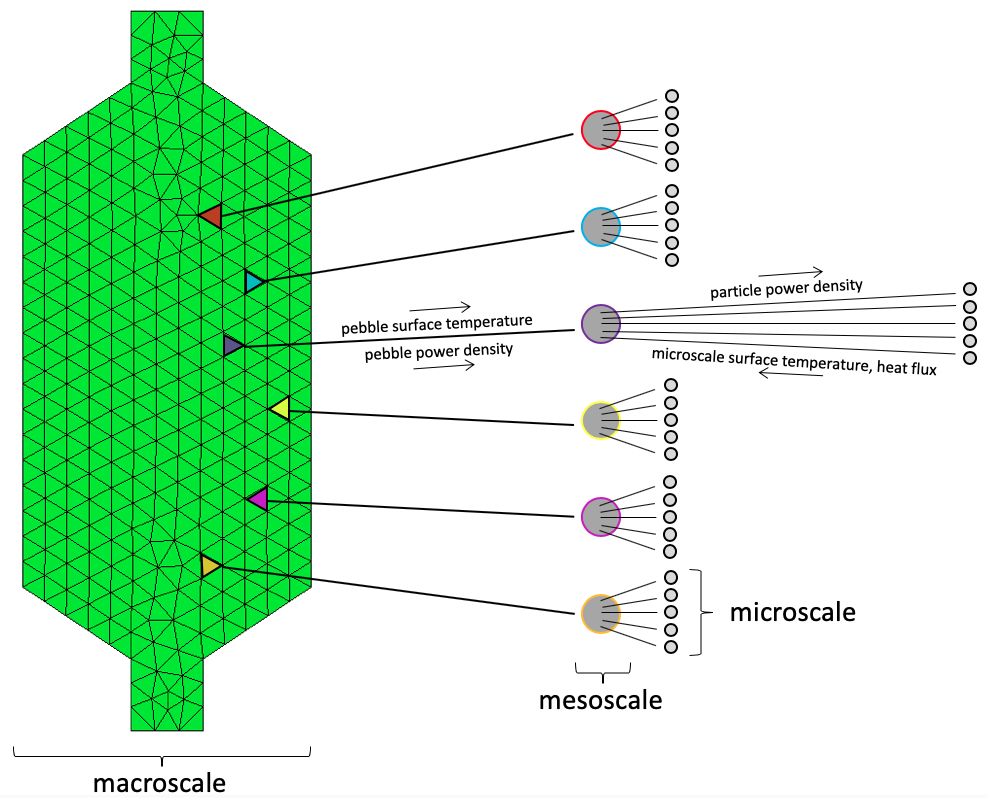
\includegraphics[width=0.8\linewidth]{figs/multiscale_pbr_d.png}
\caption{Illustration of the hierarchical multiscale execution and data transfer in Pronghorn when using the \gls{hsd} pebble model.}
\label{fig:multiscale_pbr}
\end{figure}

It is important to note that this coupling algorithm only applies to steady-state flows. An extension to transient modeling requires communication of the pebble surface heat flux to the macroscale application for use as a source term in the fluid energy conservation equation instead of the \(\alpha(T_f-T_s)\) kernel, eliminating the macroscale solid energy conservation equation. Transient capabilities are to be implemented in the near future. 

For generality, Fig.\ \ref{fig:multiscale_pbr} shows a number of microscale simulations in each pebble. As discussed in Section \ref{sec:mesomicro}, the thin fuel-matrix region of the \gls{pbfhr} modeled in Chapter \ref{sec:pbfhr} warrants the simplifying assumption that a single average microscale domain in each pebble captures the average particle heat transfer. Therefore, a single microscale domain is simulated in each mesoscale domain.

As compared to the \gls{hsd} model, the multiscale coupling procedure is much simpler for the \gls{hl} model due to the use of a single differential equation to describe the pebble temperature distribution. For the \gls{hl} method, the above calculation sequence replaces step 4, and all its sub-steps, with solution of the \gls{hl} model in Eq.\ \eqref{eq:oem} in a first-tier sub-application. The \gls{hl} method therefore does not involve second-tier sub-applications. 

\subsection{Newton-Krylov Nonlinear Solution}
\label{sec:nonlinear}

This section describes the solution of a nonlinear system of equations\mdash for the macroscale model, this refers to the four coupled equations in Eq.\ \eqref{eq:PorousEquations} or \eqref{eq:PrimitiveEqns}; for the mesoscale, this refers to the \gls{hl} model in Eq.\ \eqref{eq:oem} or the \gls{hsd} model in \eqref{eq:MesoscaleSolution}; and for the microscale, this refers to the \gls{hsd} model in Eq.\ \eqref{eq:MicroscaleSolution}. Notably, Pronghorn differs from many Navier-Stokes solvers in that the fluid conservation equations are solved together in the same matrix system, rather than with segregated solvers such as \gls{simple}.

A Newton-Krylov method is used to solve the \gls{fe} discretized forms of the multiscale models presented in Section \ref{sec:weak_form} with the \gls{supg} stabilization terms given in Section \ref{sec:supg}. The nonlinear system of equations is a root-finding problem; extending Eq.\ \eqref{eq:residual} to the discretized case, this nonlinear system is

\beq
\label{eq:nonlinear2}
\vec{R}(\vec{u})=0\ ,
\eeq

\noindent where \(\vec{R}\) is the discrete nonlinear residual vector and \(\vec{u}\) is the discrete approximate nonlinear solution. A Newton-Krylov method first linearizes Eq.\ \eqref{eq:nonlinear2} to the form

\beq
\label{eq:linear}
\textbf{A}\vec{x}=\vec{b}\ ,
\eeq

\noindent where \(\textbf{A}\) is a matrix, \(\vec{x}\) is the linear solution vector, and \(\vec{b}\) is the \gls{rhs} vector; linearization with Newton's method is explained shortly. Following this linearization, the Newton-Krylov method involves two main loops\mdash 1)~an inner loop with index \(k\) that iteratively solves for \(\vec{x}\) in Eq.\ \eqref{eq:linear}; and 2)~an outer loop with index \(i\) that iteratively solves for \(\vec{u}\) in Eq.\ \eqref{eq:nonlinear2}.

Linearization is performed with Newton's method by forming a Taylor series approximation about the current nonlinear iterate,

\beq
\label{eq:TaylorSeriesResidual}
\vec{R}(\vec{u}_{i+1})=\vec{R}(\vec{u}_i)+\frac{\partial\vec{R}(\vec{u}_i)}{\partial \vec{u}}(\vec{u}_{i+1}-\vec{u}_i)+\mathcal{O}(\vec{u}_{i+1}-\vec{u}_i)^2\ .
\eeq

\noindent Setting Eq.\ \eqref{eq:TaylorSeriesResidual} to zero and neglecting higher-order terms, a linear form is obtained,

\beq
\label{eq:linear3}
\textbf{J}(\vec{u}_i)\vec{\delta}_i=-\vec{R}(\vec{u}_i)\ ,
\eeq

\noindent where \(\textbf{J}(\vec{u}_i)\) is the Jacobian of the \(i\)-th iterate, defined as

\beq
\label{eq:JacobianDef}
\textbf{J}(\vec{u}_i)\equiv\frac{\partial \vec{R}(\vec{u}_i)}{\partial\vec{u}}\ ,
\eeq

\noindent and \(\vec{\delta}_i\) is the update vector, defined as

\beq
\label{eq:update}
\vec{\delta}_i\equiv\vec{u}_{i+1}-\vec{u}_i\ .
\eeq

\noindent Comparing Eq.\ \eqref{eq:linear3} with the general linear form in Eq.\ \eqref{eq:linear} shows that \textbf{A} represents \(\textbf{J}\), \(\vec{b}\) represents \(-\vec{R}\), and \(\vec{x}\) represents \(\vec{\delta}_i\). To match the convention used in most linear algebra texts, the notation in Eq.\ \eqref{eq:linear} is used in the remainder of this section to describe the linear problem in Eq.\ \eqref{eq:linear3}.

To summarize the Newton-Krylov method, the inner loop iteratively solves for \(\vec{x}_k\) until the norm of the linear residual in the \(k\)-th iteration, \(\vec{r}_k\), is less than a specified tolerance \(\varepsilon_l\),

\beq
\label{eq:convergence_linear}
\|\vec{r}_k\|\leq\varepsilon_l\ ,
\eeq 

\noindent where

\beq
\label{eq:linear_residual}
\vec{r}_k\equiv\textbf{A}\vec{x}_k-\vec{b}\ .
\eeq

\noindent After the linear iterations have converged, the \((i+1)\)-th nonlinear iterate is calculated as

\beq
\vec{u}_{i+1}=\vec{u}_i+\vec{x}_k\ .
\eeq

\noindent The matrix \(\textbf{A}\) and \gls{rhs} vector \(\vec{b}\) are then updated based on \(\vec{u}_{i+1}\), and the process repeated to obtain the next nonlinear iterate \(\vec{u}_{i+2}\). 

The nonlinear problem is converged once the norm of the nonlinear residual in the \(i\)-th iteration is less than a specified tolerance \(\varepsilon_n\),

\beq
\|\vec{R}(\vec{u}_i)\|\leq\varepsilon_n\ .
\eeq

\noindent The \gls{gmres} method, a Krylov subspace iterative method commonly used to solve non-symmetric linear systems, is used for solution of Eq.\ \eqref{eq:linear} \cite{saad}. A Krylov space is a vector space built by repeatedly applying a matrix to a vector. The Krylov space \(\mathcal{K}_k\) built by repeatedly applying \(\textbf{A}\) to \(\vec{r}_0\) is

\begin{equation}
\label{eq:krylov_space}
\mathcal{K}_k=\textrm{span}\{\vec{r}_0, \textbf{A}\vec{r}_0, \cdots, \textbf{A}^{k-1}\vec{r}_0\}\ .
\end{equation}

\noindent In each linear iteration, the \gls{gmres} method computes the \((k+1)\)-th linear iterate from the space \(\vec{x}_0+\mathcal{K}_k\) by minimizing the L$^2$ norm of the linear residual over \(\vec{x}_0+\mathcal{K}_k\). 

The convergence of iterative linear solvers such as \gls{gmres} generally depends on the condition number and location and clustering of the eigenvalues of \textbf{A} \cite{trefethen}. The total number of linear iterations can be dramatically reduced by preconditioning the linear system, or applying a preconditioner matrix \textbf{M} in such a way as to reduce the condition number and/or shift the eigenvalue spectrum \cite{benzi}. \gls{gmres} and other linear solvers based on minimizing residuals typically employ a ``right'' preconditioning process, which applies \textbf{M} to the linear system in Eq.\ \eqref{eq:linear} as

\beq
\textbf{A}\textbf{M}^{-1}(\textbf{M}\vec{x})=\vec{b}\ ,
\eeq

\noindent so that the residual is unchanged. \gls{petsc} options are exposed directly to \gls{moose} applications, enabling the use of a large set of preconditioners \cite{petsc}. Preconditioner selection is often problem-specific, but an \gls{asm} \gls{smp} with \gls{ilu} on sub-blocks is often sufficient.

\gls{ad}, sometimes referred to as ``algorithmic differentiation,'' is used to calculate the Jacobians in Eq.\ \eqref{eq:JacobianDef} \cite{ad}. Operator overloads are defined for all of the fundamental arithmetic operators, such as addition, subtraction, multiplication, and division, as well as for elementary functions such as exponentials and logarithms. These overloads then systematically apply the chain rule to the sequence of arithmetic operations used to construct the residual \(\vec{R}\) to compute a working precision accurate estimate of the derivatives of \(\vec{R}\) with respect to \(\vec{u}\). The use of \gls{ad} enables faster application development by avoiding the by-hand derivation of nonlinear residual derivatives. In many cases, \gls{ad} also decreases the number of linear and nonlinear iterations due to the more accurate Jacobian evaluation. The use of \gls{ad} also allows seamless interchange between different sets of solution variables without any modifications to the kernel and \gls{bc} classes that would otherwise be required for by-hand Jacobian evaluation.

\section{Software Engineering Design}
\label{sec:software}
% TODO: change many to all?

High-quality software is essential to support the safety analysis of nuclear reactors. The \gls{moose} framework meets many \gls{nqa1} standards that certify software providing safety functions for nuclear facilities. The \gls{moose} framework meets these standards through supporting a software engineering design incorporating the use of git version control, GitHub pull requests and peer review, \gls{ci} with regression and unit tests of the framework and registered applications, and code style and formatting requirements \cite{slaughter}. Pronghorn shares many of these software engineering best practices, including\mdash

\begin{itemize}
\itemsep0.3em
\item \gls{inl} GitLab repository with issue tracking and peer review of all proposed changes;
\item \gls{ci} with a regression and Googletest unit test suite to ensure proper application behavior before new feature addition to both Pronghorn and the \gls{moose} framework;
\item Hierarchical \gls{xml} input file syntax;
\item In-source \texttt{C++} Doxygen documentation;
\item In-source Markdown for rendering a navigable user guide as a \gls{html} web page; and
\item In-repository theory manual.
\end{itemize}

Select examples from Pronghorn's regression and unit test suite are described at greater length in Chapter \ref{sec:vv}.


\chapter{Pronghorn Model Verification}
\label{sec:vv}

The use of computational models to predict reactor response to nominal and off-normal conditions requires high software quality and a strong \gls{vv} base. The integrated documentation, use of version control systems, and \gls{ci} testing discussed in Section \ref{sec:software} ensure high software reliability, efficiency, and maintainability. Equally important is the establishment of a set of verification tests and validation benchmarks relevant to the software's intended application space. 

Efforts underway at \gls{inl} and \gls{ucb} focus on building a comprehensive software test matrix to support qualification of Pronghorn for single-phase \gls{pbr} simulations. The objective of this section is to describe a small subset of these verification tests in order to 1)~emphasize the rigor in the numerical implementation of the models in Chapter \ref{sec:PhysicalModels} and 2)~support the application of Pronghorn to low-speed gas-cooled pebble experiments in Chapter \ref{sec:sana} and to salt-cooled \glspl{pbr} in Chapter \ref{sec:pbfhr}. Additional verification exercises such as the code-to-code \gls{oecd} \gls{pbmr} benchmark and code-to-code comparisons against STAR-CCM+ are described at length elsewhere \cite{balestra,lee_2020}.

This chapter is organized as follows. Section \ref{sec:mms} discusses the use of the \gls{mms} to verify correct source implementation of all kernels and \glspl{bc}. The rigorous developer-imposed requirement to satisfy theoretical convergence rates for all source objects reflects the high caliber of the physics implementation, an essential first step before conducting more complex analyses.

The focus of Chapters \ref{sec:sana} and \ref{sec:pbfhr} are on porous flows, but many the pebble region of most \glspl{pbr} is adjacent to an open plenum that falls under the purview of a \gls{th} core simulator such as Pronghorn. \gls{th} models of \glspl{pbr} must be able to accurately predict fluid mixing in the plenum region and the resulting thermal stresses on core structural materials. The macroscale models derived in Chapter \ref{sec:PhysicalModels} reduce to equations applicable to open flows by setting \(\epsilon=1\), \(W=0\), \(\tilde{\mu}=\mu_f\), \(\alpha=0\), \(\kappa_f=k_f\), and \(\kappa_s=k_s\). To contrast with the porous simulations in Chapters \ref{sec:sana} and \ref{sec:pbfhr} and to verify the macroscale models for open flows such as plena, Sections \ref{sec:natural_convection} and \ref{sec:potential_flow} demonstrate application of the porous macroscale models to open flows with thermal and flow characteristics relevant to \glspl{pbr}.

Section \ref{sec:natural_convection} presents Pronghorn simulations of a numerical benchmark defined by de Vahl Davis and Jones for viscous natural convection flow in a square enclosure \cite{davis}. Many \gls{pbr} designs incorporate natural convection cooling in shutdown conditions, and this benchmark is an indication of the macroscale model's capabilities for modeling thermally-driven natural convection.

Section \ref{sec:potential_flow} presents Pronghorn simulations of inviscid flow over a cylinder. Most gas-cooled \glspl{pbr} operate at high Reynolds number, making inviscid flow models a reasonable simplification over viscous models and their accompanying boundary layer meshing requirements. In the limit of zero Mach number, the compressibility effects in the macroscale model become insignificant, allowing a comparison to the analytic incompressible potential flow solution for inviscid cylinder flow. This analysis therefore serves as a demonstration of the macroscale model's capabilities for modeling inviscid flow and compressibility effects that may be quite significant in gas-cooled systems with large core temperature rises \cite{martineau}.

All of the analyses in Chapters \ref{sec:sana} and \ref{sec:pbfhr} use the friction-dominated macroscale model in Eq. \eqref{eq:PrimitiveEqns} due to its more robust convergence properties and faster runtime relative to the Navier-Stokes model in Eq. \eqref{eq:PorousEquations}. The verification tests presented in Sections \ref{sec:natural_convection} and \ref{sec:potential_flow} therefore provide a diversity to the macroscale model applications in this dissertation and demonstrate Pronghorn's capacity as a general-purpose flow solver.
% However, the Navier-Stokes macroscale model in Eq. \eqref{eq:PorousEquations} is expected to be more accurate than the friction-dominated model for prototypical gas-cooled \gls{pbr} systems and coupled bed-plenum geometries due to the higher flowrates and more significant mixing effects.

To enable reproduction of the simulations presented in this chapter, Appendix \ref{sec:reproducibility} lists all data and input files related to this chapter.

\section{Method of Manufactured Solutions}
\label{sec:mms}

The \gls{mms} is used to verify correct source code implementation of all contributions to the residuals in Eqs. \eqref{eq:PronghornEquations_V2WeakForm} and \eqref{eq:PrimitiveWeakForms}\mdash that is, all kernels and \gls{bc} objects.

A user-specified solution to a particular governing equation is ``manufactured'' by adding an appropriate forcing term to that equation \cite{roache}. For example, the diffusion equation with unity diffusivity has the strong form

\begin{equation}
\label{eq:diff_example}
-\nabla^2\Phi=0\ ,
\end{equation}
 
\noindent where \(\Phi\) is the solution variable. For a manufactured solution of the form

\begin{equation}
\label{eq:mms_soln}
\Phi=f(\vec{x},t)\ ,
\end{equation}

\noindent where \(f\) is a generic function, solution of the modified equation

\begin{equation}
-\nabla^2\Phi=-\nabla^2f(\vec{x},t)
\end{equation}

\noindent with the appropriate \glspl{bc} on \(\Phi\) will return the manufactured solution in Eq. \eqref{eq:mms_soln} provided the source implementation of the diffusion kernel is correct. Successively refining the mesh and/or time resolution can then be used to estimate convergence rates for various \gls{fe} basis function orders and \gls{fd} time integration schemes.

To verify spatial convergence, the L$^2$ norm relative to the manufactured solution is computed on a series of uniformly refined meshes. When measured in the L$^2$ norm, the \gls{fem} is second-order accurate in space with linear elements and third-order accurate in space with quadratic elements. 

While arbitrary manufactured solution spatial dependencies are selected for the spatial convergence tests, the temporal convergence tests manufacture solutions that are separable in time and space. Further, the spatial dependence is linear such that the use of linear \gls{fe} basis functions nearly isolates the time discretization error from the spatial discretization error. To verify temporal convergence, the spatial mesh is fixed and the L$^2$ norm relative to the manufactured solution is computed on a series of uniformly refined time step sizes. When measured in the L$^2$ norm, the time integration is first-order accurate in time with the backward Euler method and second-order accurate in time with the \gls{bdf2}, Crank-Nicolson, and \gls{dirk} methods. 

Correct source implementation is inferred by achieving these theoretical spatial and temporal convergence rates. As an example, \gls{mms} convergence rates for the (a) \(-\nabla\cdot(\kappa_s\nabla T_s)\) kernel and (b) \(\epsilon\rho_fC_{p_f}\partial T_f/\partial t\) kernel are shown in Fig.\ \ref{fig:convergence}. The expected convergence rates of 2 and 3 for linear and quadratic elements, respectively, are obtained for the spatial kernel. The expected convergence rates of 1 and 2 are obtained for the various time discretization schemes for the time-dependent kernel.

\begin{figure}[!h]
\centering
    \begin{subfigure}{0.48\linewidth}
        \centering
        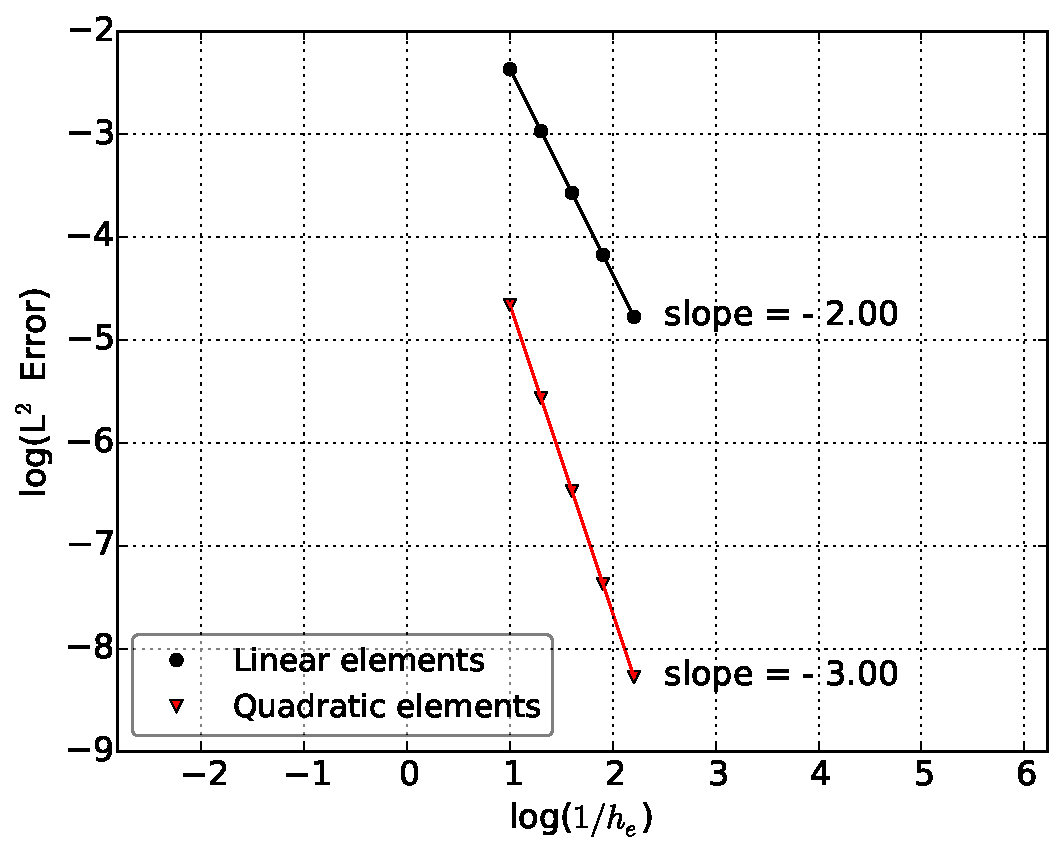
\includegraphics[width=1.0\linewidth]{figs/convergence_solid_energy_diffusion.pdf}
       \caption{\gls{mms} test of \(-\nabla\cdot \left(\kappa_s\nabla T_s\right)\)}
    \end{subfigure}
    \begin{subfigure}{0.48\linewidth}
        \centering
        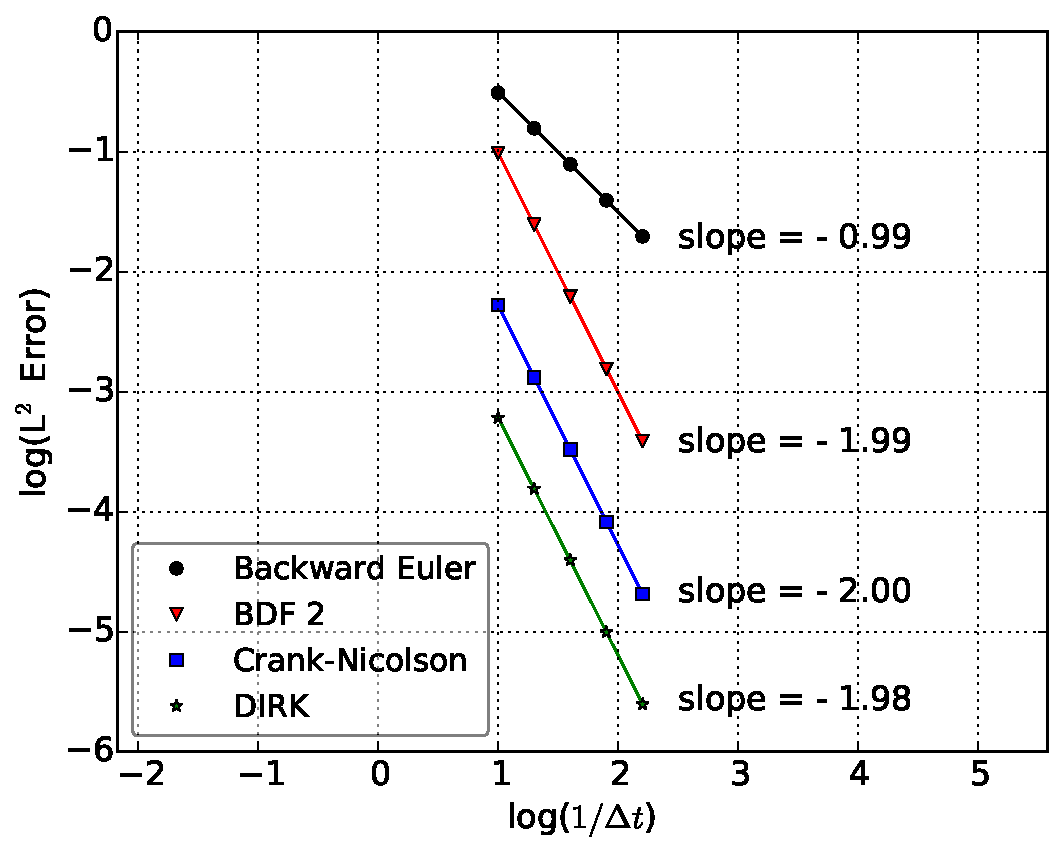
\includegraphics[width=1.0\linewidth]{figs/convergence_fluid_energy_time.pdf}
        \caption{\gls{mms} test of \(\epsilon\rho_fC_{p_f}\frac{\partial T_f}{\partial t}\)}
    \end{subfigure}
    \caption{\gls{mms} convergence studies for the (a) \(\nabla\cdot(\kappa_s\nabla T_s)\) kernel and (b) \(\epsilon\rho_fC_{p_f}\partial T_f/\partial t\) kernel. Discrete points are error measurements and solid lines are linear fits.}
    \label{fig:convergence}
\end{figure}

\section{Natural Convection in an Open Cavity}
\label{sec:natural_convection}

Many \glspl{pbr} are designed to remove decay heat via thermally-driven natural convection. The Rayleigh number \(Ra\) quantifies the relative importance of buoyant forces to diffusive forces, and is defined as

\beq
\label{eq:RaDef}
Ra\equiv\frac{|g|\rho_f^2C_{p,f}\beta_f L^3\Delta T_f}{\mu_f k_f}\ ,
\eeq

\noindent where \(\Delta T/L\) is the imposed temperature gradient in a domain of length \(L\). Provided the imposed temperature gradient is not entirely aligned with the gravitational acceleration vector, then for sufficiently large Rayleigh number, buoyant forces overcome dissipative forces to produce convective motions \cite{manneville,sandberg}.

This section presents Pronghorn simulations of flow in an open square cavity with differentially heated walls to verify the applicability of the Navier-Stokes macroscale model to open natural convection flows. This verification exercise is relevant to the use of coarse mesh tools for prediction of mixing and thermal striping in the open plena adjacent to many \gls{pbr} beds. Additional objectives of this analysis are to 1)~illustrate the reduction of the macroscale models in Chapter \ref{sec:PhysicalModels} to the open flow equations through proper selection of the macroscale closures and 2)~demonstrate mesh refinement studies for a physics simulation that are omitted in all later chapters for brevity.

The problem geometry is shown in Fig.\ \ref{fig:rb_cell}; the domain and \glspl{bc} are selected based on a benchmark defined by de Vahl Davis and Jones \cite{davis}. The cavity dimension \(L\) is 1 \si{\meter}, gravity acts in the \(-z\) direction, velocity satisfies no-slip \glspl{bc} on all surfaces, and the top and bottom boundaries are insulated. The temperature is \(T_H\) on the heated boundary and \(T_C\) on the cooled boundary. The fluid is modeled with the Navier-Stokes macroscale model in Eq. \eqref{eq:PorousEquations} with \(\epsilon=1\), \(W=0\), \(\tilde{\mu}=\mu_f\), \(\alpha=0\), \(\kappa_f=k_f\), and \(\kappa_s=k_s\) and properties closed by the ideal gas \gls{eos}. The Prandtl number is fixed at 0.71 and the Rayleigh number is varied from \(10^3\) to \(10^6\) by varying the fluid dynamic viscosity and thermal conductivity.

\begin{figure}[!h]
\centering
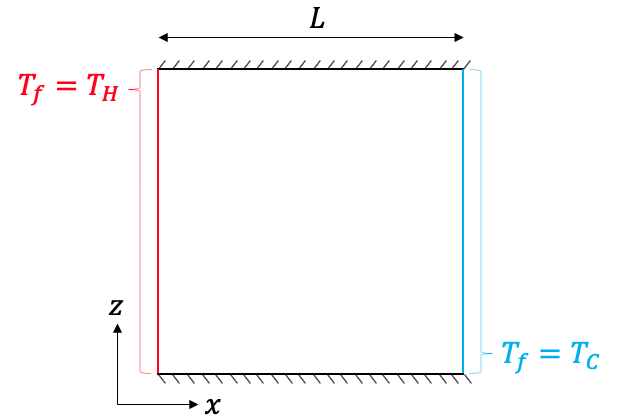
\includegraphics[width=0.5\linewidth]{figs/rb_cell.png}
\caption{Problem set-up for natural convection flow in an \(L\times L\) \si{\meter} square enclosure.}
\label{fig:rb_cell}
\end{figure}

Pronghorn predictions of velocity, temperature, and Nusselt number are compared with a reference solution distributed with the benchmark \cite{davis}. In addition to spatial velocity and temperature distributions, pointwise information requested of the original benchmark participants includes

\begin{itemize}
\itemsep0em
\item Maximum \(x\)-direction velocity on the \(x^+=0.5\) plane, \(V^+_{x,\text{max}}\), and its \(z\)-location \(z^+_u\);
\item Maximum \(y\)-direction velocity on the \(z^+=0.5\) plane, \(V^+_{z,\text{max}}\), and its \(x\)-location \(x^+_v\);
\item Maximum Nusselt number on the \(x^+=0\) plane, \(Nu_\text{max}\), and its location \(z^+_\text{max}\);
\item Minimum Nusselt number on the \(x^+=0\) plane, \(Nu_\text{min}\), and its location \(z^+_\text{min}\); and
\item Average Nusselt number \(\la Nu\ra\).
\end{itemize}

All locations, velocities, and temperatures are presented in nondimensional form by defining the following quantities,

\beq
\label{eq:nondim_x}
x^+=\frac{x}{L},\quad z^+=\frac{z}{L},\quad V_i^+=V_i\frac{\rho_f C_{p,f}L}{k_f},\quad T_f^+=\frac{T_f-T_C}{T_H-T_C}\ .
\eeq

\noindent A mesh refinement study based on a subset of the numeric information requested of benchmark participants is shown in Fig.\ \ref{fig:mr}. For each Rayleigh number, the same starting mesh is uniformly refined until the L$^1$ norm of the error in each of the scalar metrics is less than 5\%. A total of five meshes are considered, with errors computed relative to the to obtain all further results.

\begin{figure}[!h]
\centering
\begin{subfigure}{0.48\textwidth}
  \centering
  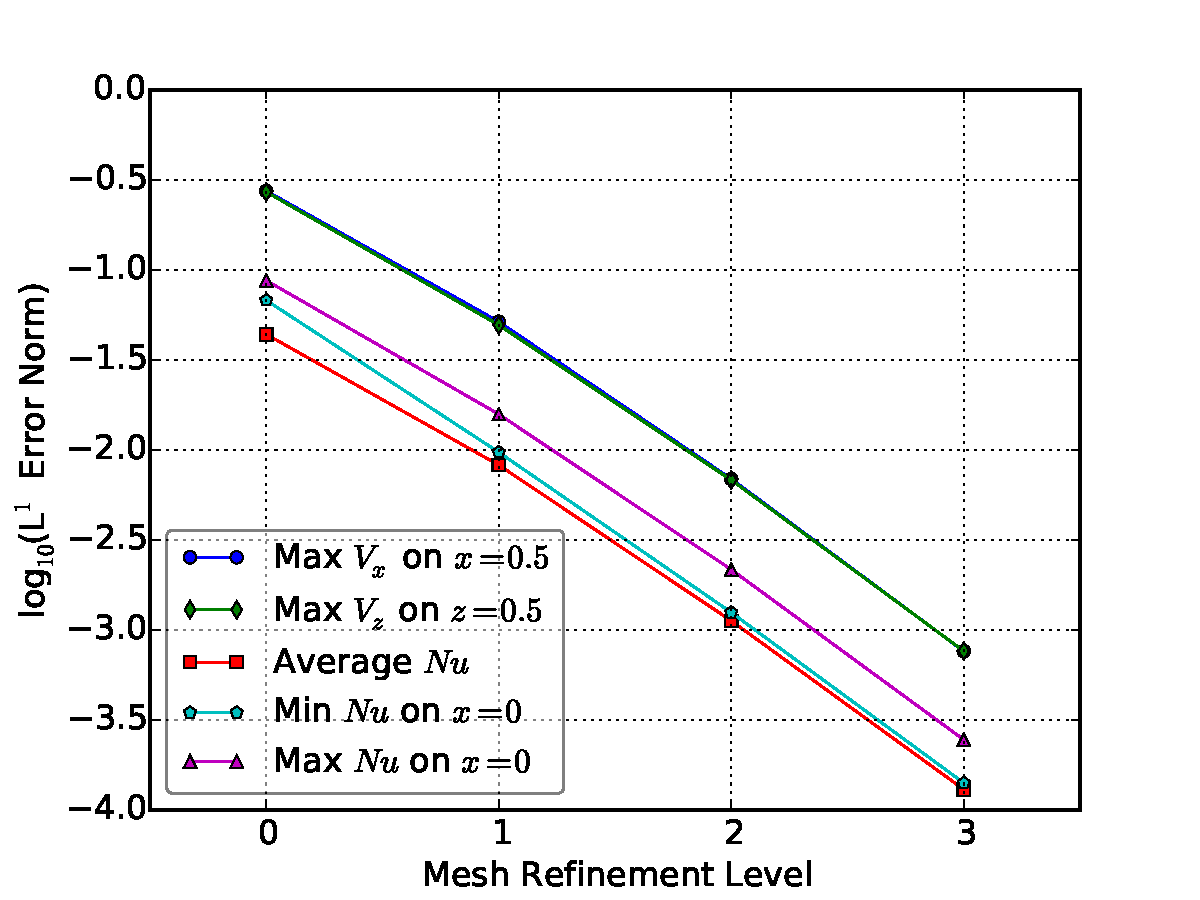
\includegraphics[width=\linewidth]{../../pronghorn/doc/laminar_flow/figs/Ra1000_mr.pdf}
  \caption{\(Ra=10^3\)}
  \label{fig:mr1}
\end{subfigure}
\begin{subfigure}{0.48\textwidth}
  \centering
  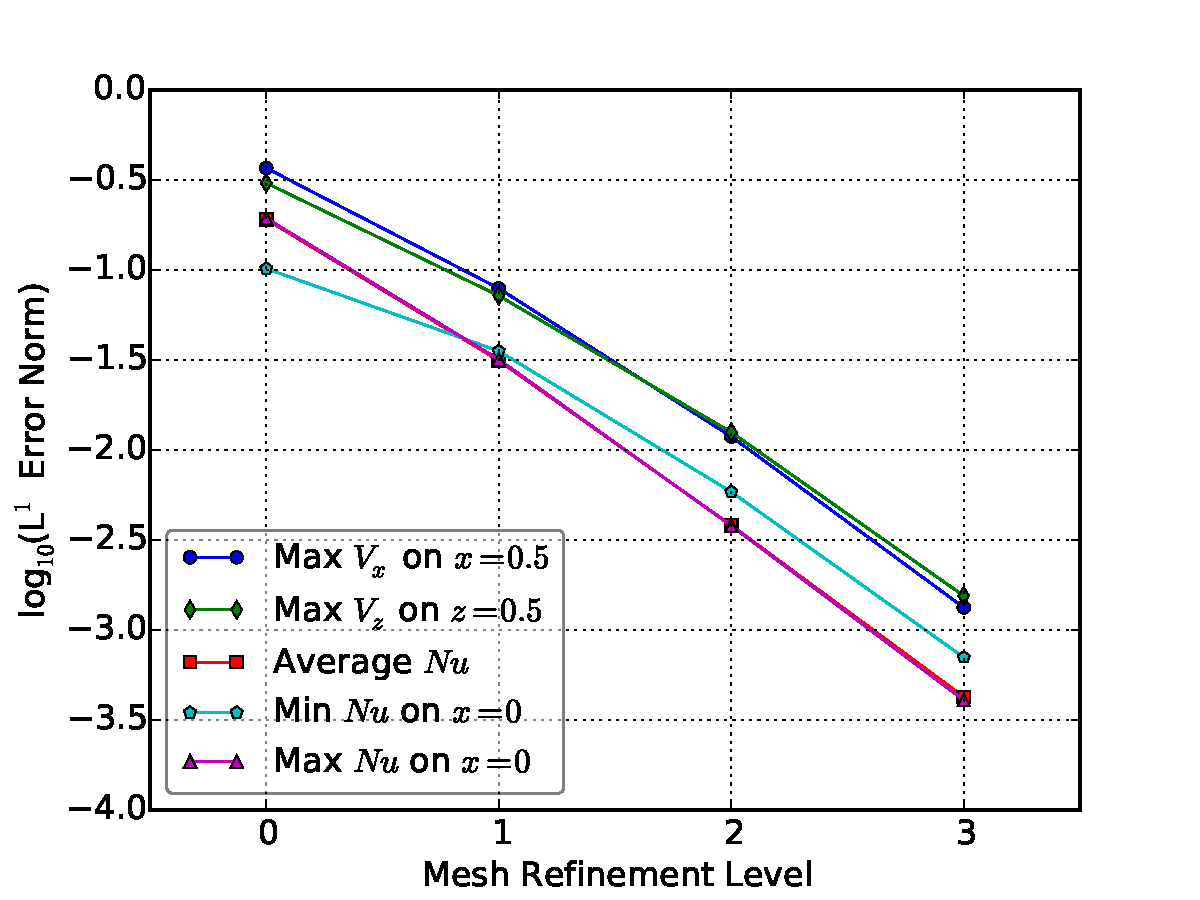
\includegraphics[width=\linewidth]{../../pronghorn/doc/laminar_flow/figs/Ra10000_mr.pdf}
  \caption{\(Ra=10^4\)}
  \label{fig:mr2}
\end{subfigure}
\begin{subfigure}{0.48\textwidth}
  \centering
  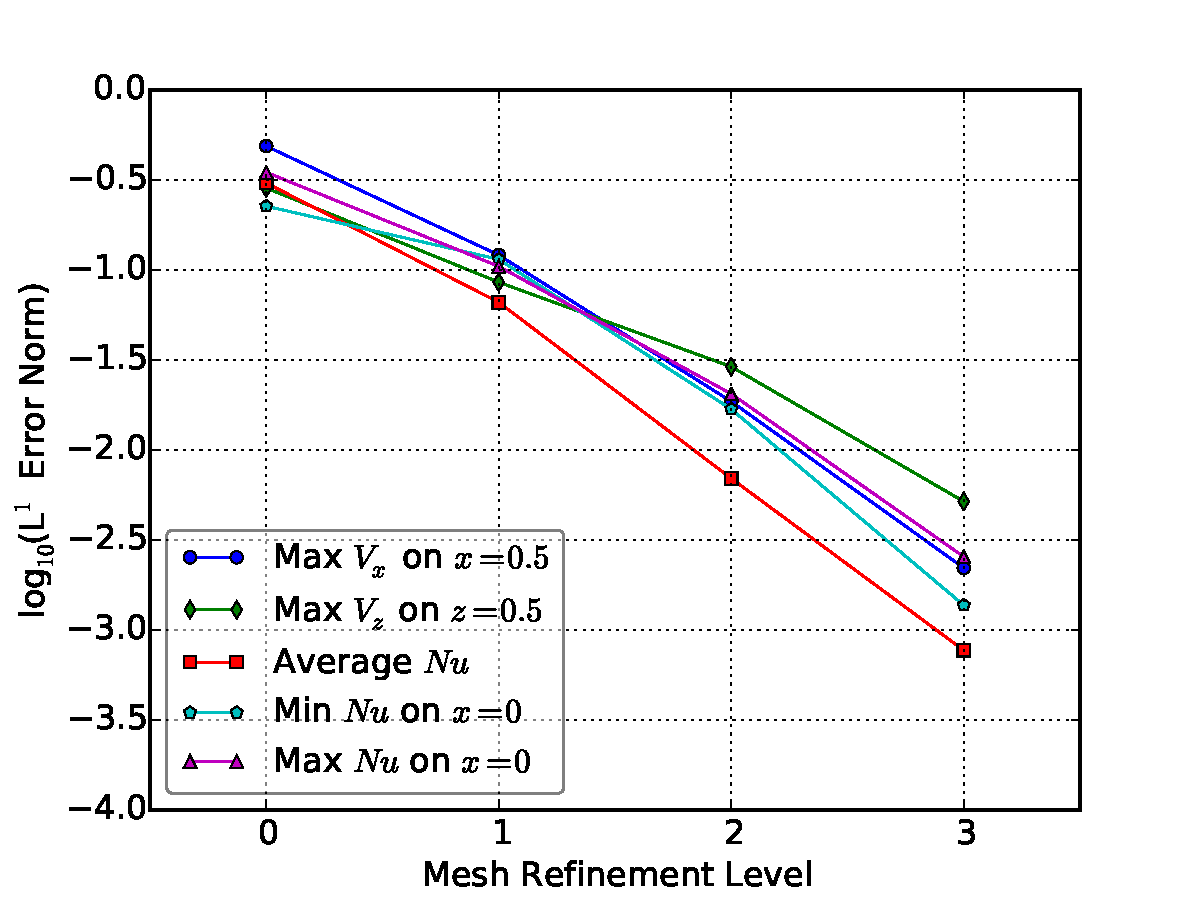
\includegraphics[width=\linewidth]{../../pronghorn/doc/laminar_flow/figs/Ra100000_mr.pdf}
  \caption{\(Ra=10^5\)}
  \label{fig:mr3}
\end{subfigure}
\begin{subfigure}{0.48\textwidth}
  \centering
  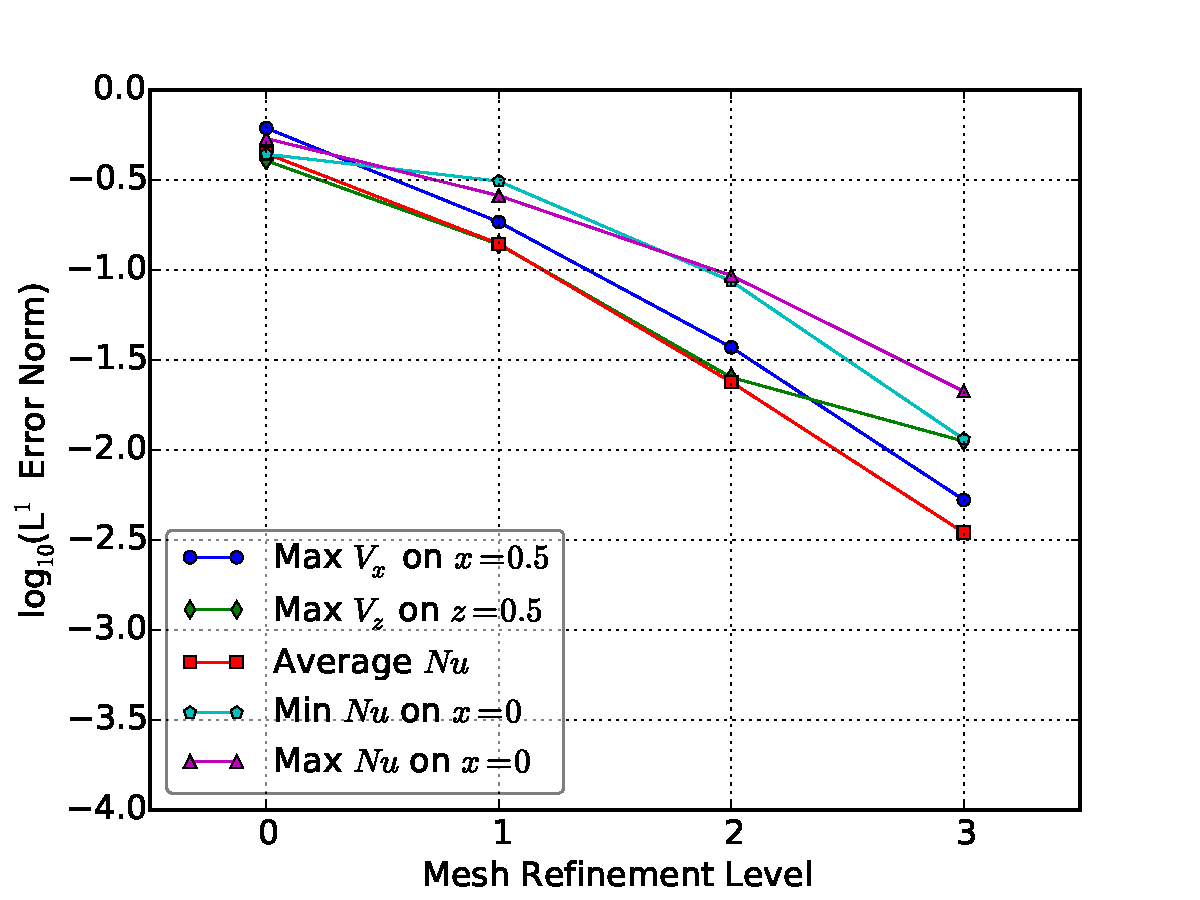
\includegraphics[width=\linewidth]{../../pronghorn/doc/laminar_flow/figs/Ra1000000_mr.pdf}
  \caption{\(Ra=10^6\)}
  \label{fig:mr4}
\end{subfigure}
\caption{L$^1$ error norm of scalar benchmark metrics as a function of the mesh refinement.}
\label{fig:mr}
\end{figure}

Fig.\ \ref{fig:rb_results} shows Pronghorn predictions of fluid temperature, \(x\)-direction velocity, and \(z\)-direction velocity with contours in white for Rayleigh numbers of \(10^3\), \(10^4\), \(10^5\), and \(10^6\). For all cases, the decrease in density along the hot surface causes the fluid to rise along the left wall, while the increase in density along the cool surface causes the fluid to sink along the right wall. 

As the Rayleigh number increases, the thickness of the thermal boundary layer on the hot and cool surfaces becomes thinner, the fluid motion becomes more chaotic, and the heat flux between the vertical cavity walls increases. For higher Rayleigh numbers, the largest \(z\)-velocity magnitudes occur in thinner regions near the vertical walls, while the increased momentum of the vertical flows causes the regions of large \(x\)-velocity magnitudes to move closer to the corners of the cavity. Excellent qualitative agreement in temperature and velocity is obtained with the reference solution \cite{davis_1983}.

\begin{figure}[!h]
\centering
\begin{subfigure}{0.32\textwidth}
  \centering
  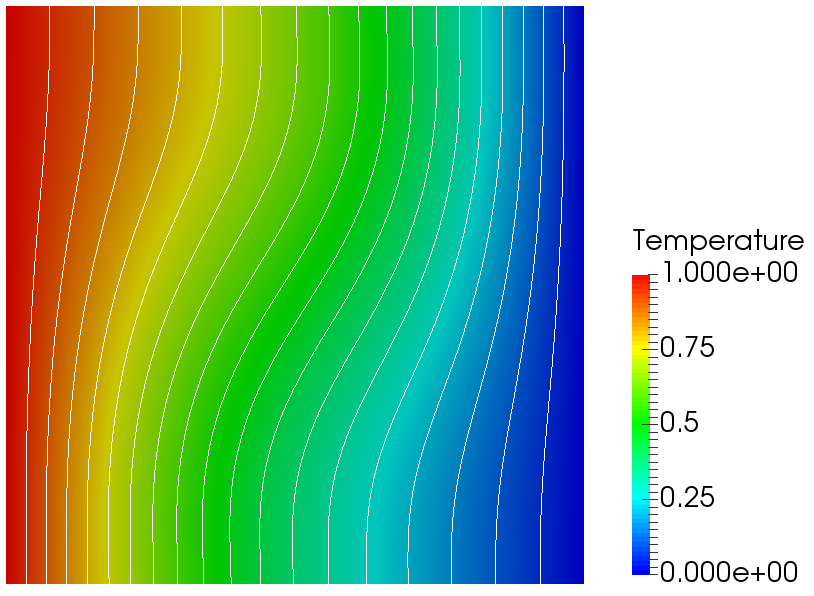
\includegraphics[width=\linewidth]{../../pronghorn/doc/laminar_flow/figs/Ra3_t.png}
  \caption{\(T_f^+\), \(Ra=10^3\)\color{white}1234}
    \vspace*{0.5em}
\end{subfigure}
\begin{subfigure}{0.32\textwidth}
  \centering
  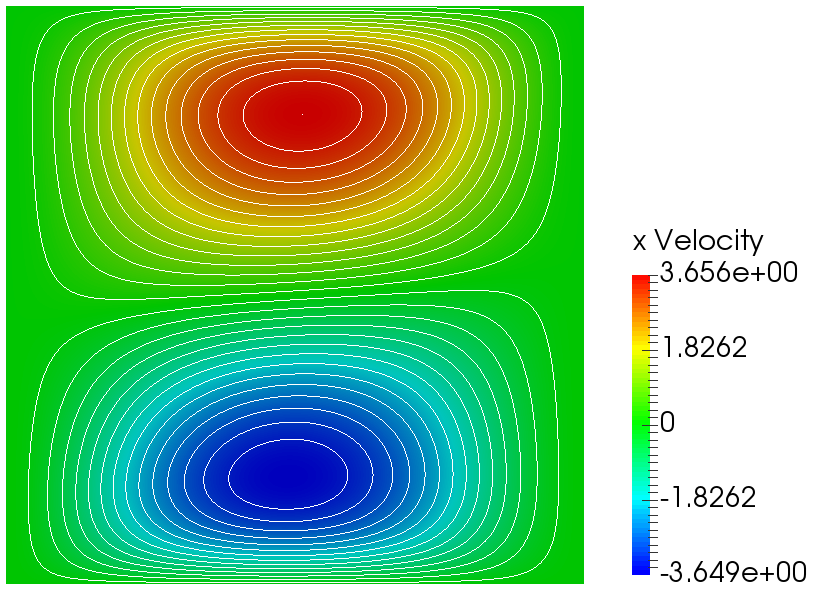
\includegraphics[width=\linewidth]{../../pronghorn/doc/laminar_flow/figs/Ra3_u.png}
  \caption{\(V_x^+\), \(Ra=10^3\)\color{white}1234}
    \vspace*{0.5em}
\end{subfigure}
\begin{subfigure}{0.32\textwidth}
  \centering
  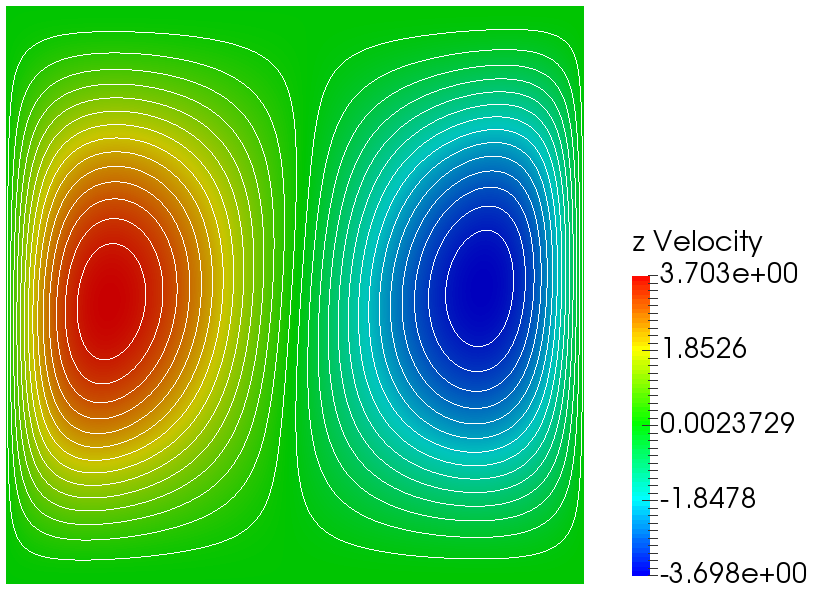
\includegraphics[width=\linewidth]{../../pronghorn/doc/laminar_flow/figs/Ra3_v.png}
  \caption{\(V_z^+\), \(Ra=10^3\)\color{white}1234}
  \vspace*{0.5em}
\end{subfigure}
\begin{subfigure}{0.32\textwidth}
  \centering
  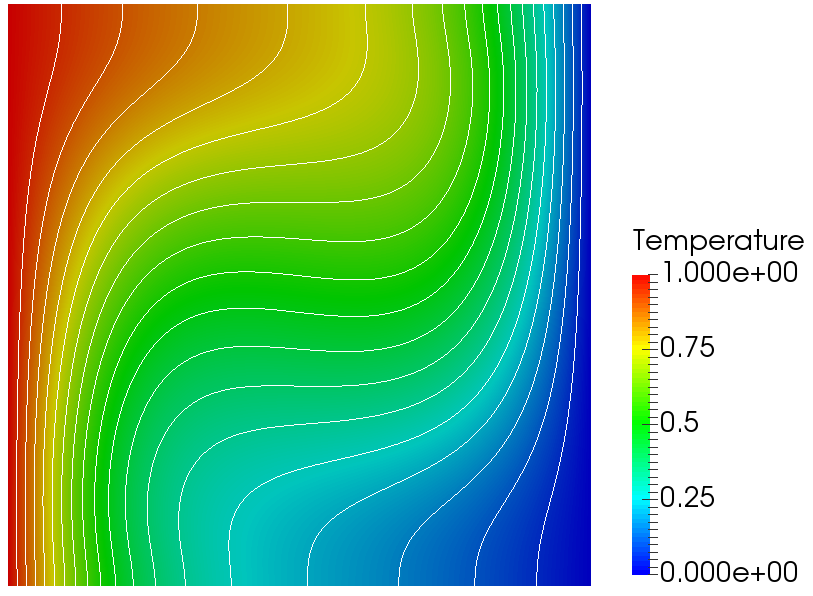
\includegraphics[width=\linewidth]{../../pronghorn/doc/laminar_flow/figs/Ra4_t.png}
  \caption{\(T_f^+\), \(Ra=10^4\)\color{white}1234}
    \vspace*{0.5em}
\end{subfigure}
\begin{subfigure}{0.32\textwidth}
  \centering
  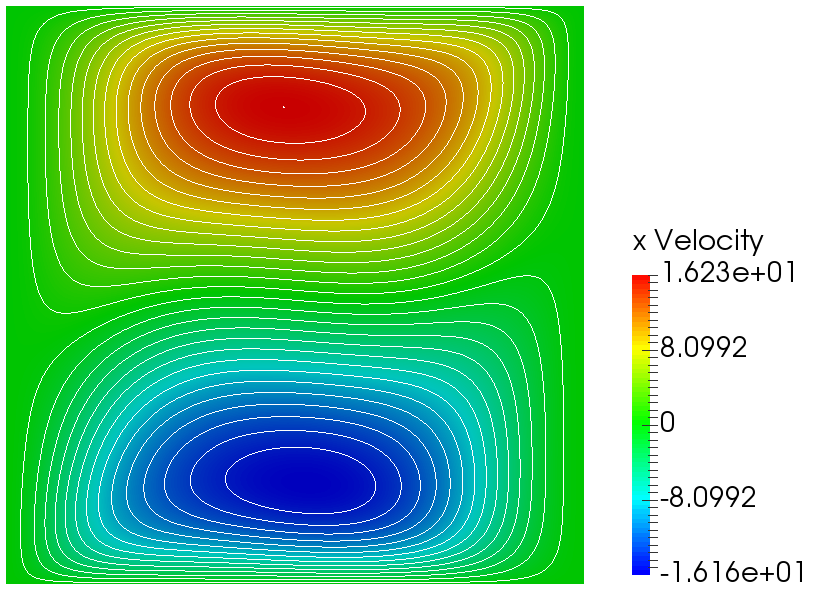
\includegraphics[width=\linewidth]{../../pronghorn/doc/laminar_flow/figs/Ra4_u.png}
  \caption{\(V_x^+\), \(Ra=10^4\)\color{white}1234}
    \vspace*{0.5em}
\end{subfigure}
\begin{subfigure}{0.32\textwidth}
  \centering
  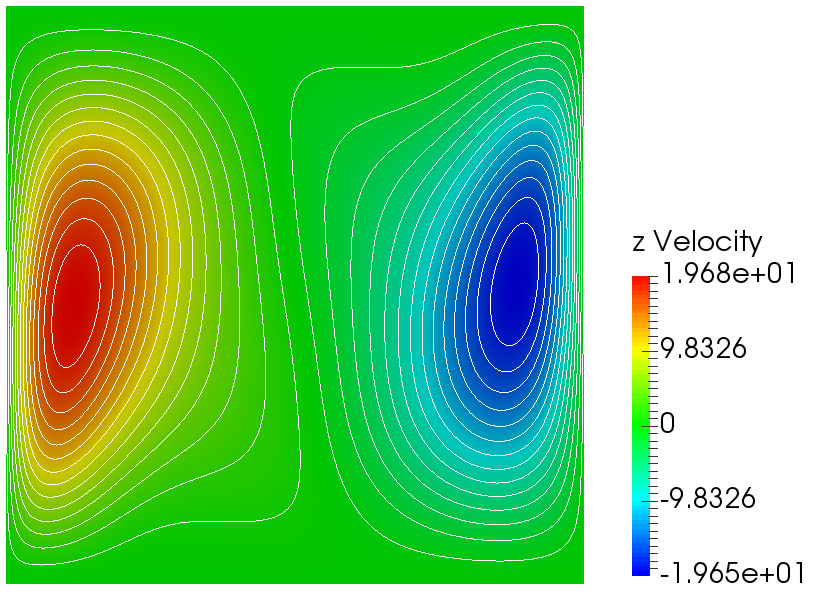
\includegraphics[width=\linewidth]{../../pronghorn/doc/laminar_flow/figs/Ra4_v.png}
  \caption{\(V_z^+\), \(Ra=10^4\)\color{white}1234}
    \vspace*{0.5em}
\end{subfigure}
\begin{subfigure}{0.32\textwidth}
  \centering
  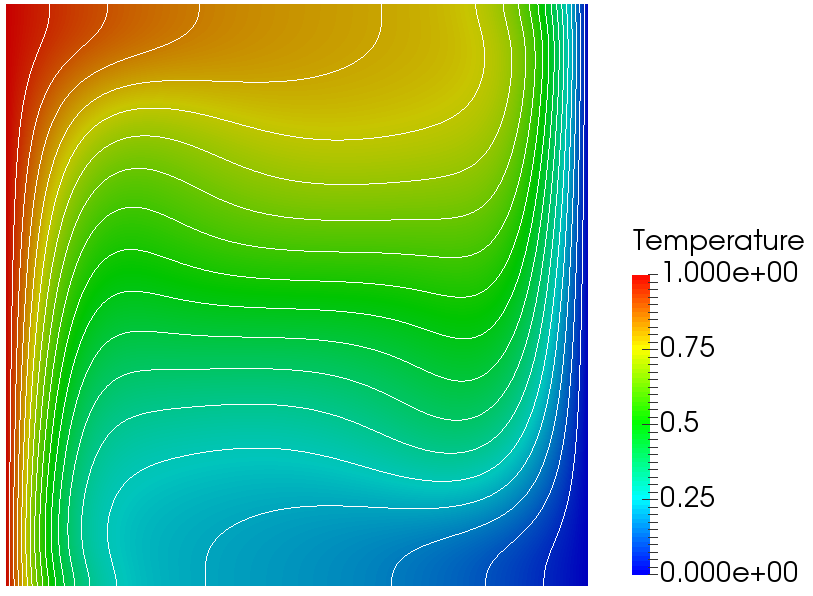
\includegraphics[width=\linewidth]{../../pronghorn/doc/laminar_flow/figs/Ra5_t.png}
  \caption{\(T_f^+\), \(Ra=10^5\)\color{white}1234}
    \vspace*{0.5em}
\end{subfigure}
\begin{subfigure}{0.32\textwidth}
  \centering
  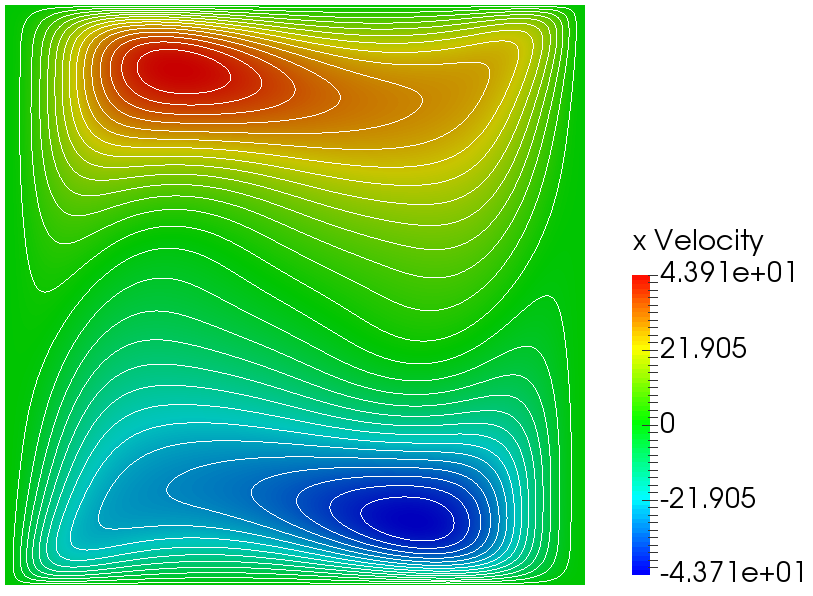
\includegraphics[width=\linewidth]{../../pronghorn/doc/laminar_flow/figs/Ra5_u.png}
  \caption{\(V_x^+\), \(Ra=10^5\)\color{white}1234}
    \vspace*{0.5em}
\end{subfigure}
\begin{subfigure}{0.32\textwidth}
  \centering
  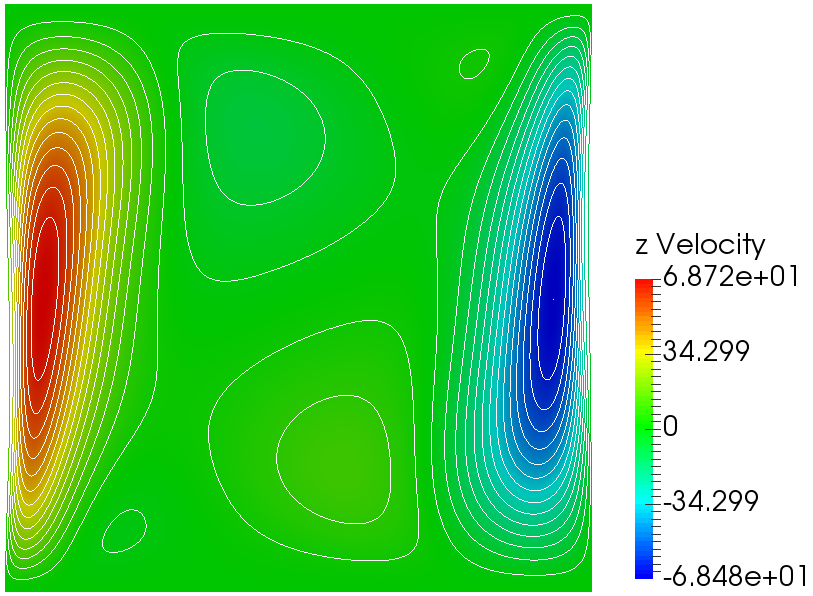
\includegraphics[width=\linewidth]{../../pronghorn/doc/laminar_flow/figs/Ra5_v.png}
  \caption{\(V_z^+\), \(Ra=10^5\)\color{white}1234}
    \vspace*{0.5em}
\end{subfigure}
\begin{subfigure}{0.32\textwidth}
  \centering
  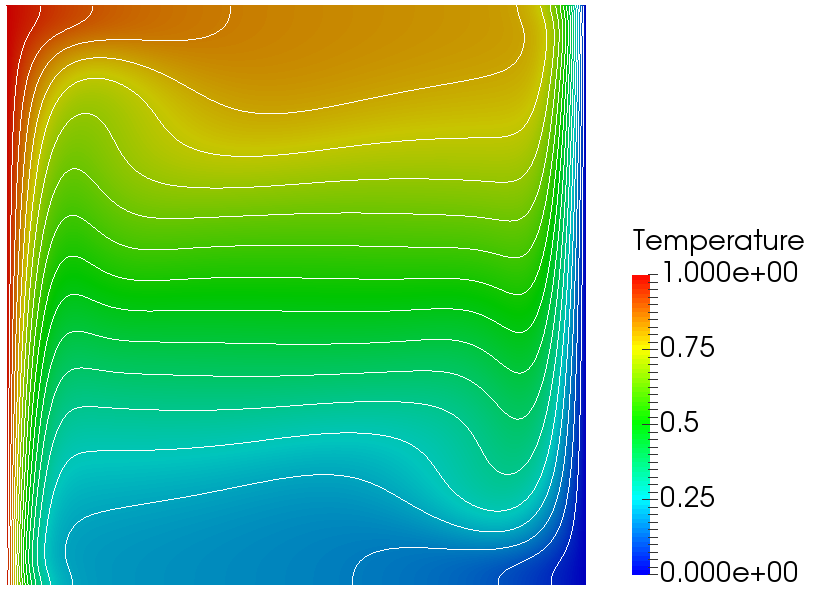
\includegraphics[width=\linewidth]{../../pronghorn/doc/laminar_flow/figs/Ra6_t.png}
  \caption{\(T_f^+\), \(Ra=10^6\)\color{white}1234}
  \label{fig:Ra6T}
    \vspace*{0.5em}
\end{subfigure}
\begin{subfigure}{0.32\textwidth}
  \centering
  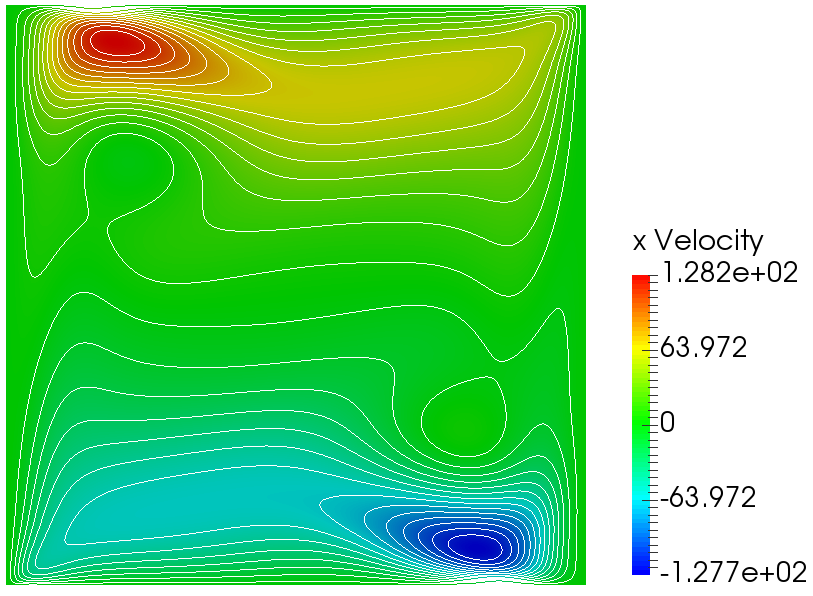
\includegraphics[width=\linewidth]{../../pronghorn/doc/laminar_flow/figs/Ra6_u.png}
  \caption{\(V_x^+\), \(Ra=10^6\)\color{white}1234}
  \label{fig:Ra6u}
    \vspace*{0.5em}
\end{subfigure}
\begin{subfigure}{0.32\textwidth}
  \centering
  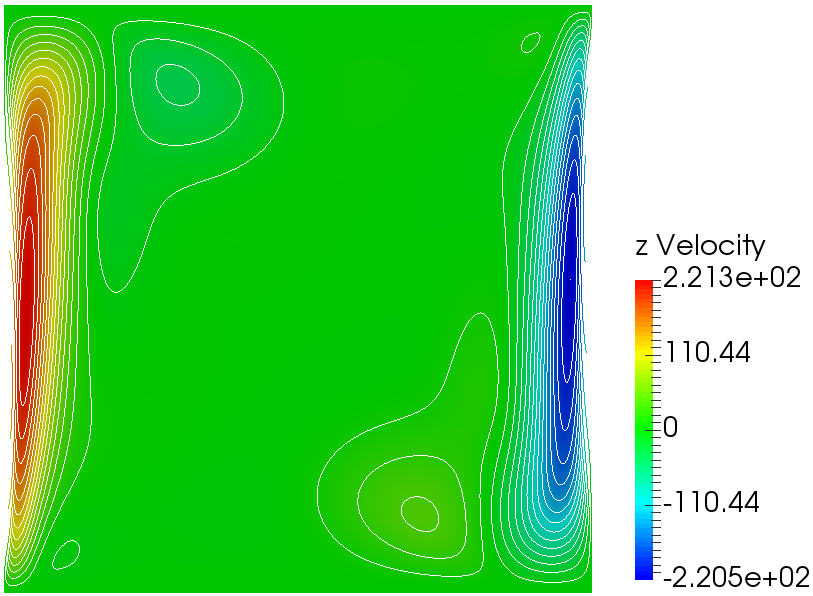
\includegraphics[width=\linewidth]{../../pronghorn/doc/laminar_flow/figs/Ra6_v.png}
  \caption{\(V_z^+\), \(Ra=10^6\)\color{white}1234}
  \label{fig:Ra6v}
    \vspace*{0.5em}
\end{subfigure}
\caption{Pronghorn predictions of \(T_f^+\), \(V_x^+\), and \(V_z^+\) for \mbox{(a -- c)} \(Ra=10^3\), \mbox{(d -- f)} \(Ra=10^4\), \mbox{(g -- i)} \(Ra=10^5\), and \mbox{(j -- l)} \(Ra=10^6\).}
\label{fig:rb_results}
\end{figure}

Table \ref{table:rb} provides a quantitative comparison between the Pronghorn and reference solutions for the scalar benchmark metrics. Given the limited significant figures reported in the benchmark, some relative errors are zero. For most data points, Pronghorn agrees with the reference solution to less than 1\% relative error. The largest relative errors, observed in the predictions for \(z^+_\text{max}\), represent absolute errors on the order of 0.001. When expressed in dimensional form with Eq. \eqref{eq:nondim_x}, the absolute error in this \(z_\text{max}\) for \(L=1\) \si{\meter} is only 1 \si{\milli\meter}.

\begin{table}[!h]
\caption{Pronghorn (PH) and reference (Ref.) solutions for the natural convection benchmark \cite{davis_1983} with percent error (Err.) between Pronghorn and the reference.} 
\centering
\footnotesize
\centerline{
\begin{tabular}{|c|c c >{\bfseries}c |c c >{\bfseries}c| c c >{\bfseries}c| c c >{\bfseries}c|}
\hline\hline
 & \multicolumn{3}{c|}{\color{white}${\rvert^\dagger}^\dagger$\color{black}\(Ra=10^3\)\color{white}${\rvert^\dagger}^\dagger$\color{black}} & \multicolumn{3}{c|}{\(Ra=10^4\)} &  \multicolumn{3}{c|}{\(Ra=10^5\)} &  \multicolumn{3}{c|}{\(Ra=10^6\)}\Bstrut\\\cline{2-13}
 & Ref. & PH & Err. & Ref. & PH & Err. & Ref. & PH & Err. & Ref. & PH & Err.\Tstrut\Bstrut\\
\hline
\(V^+_{x,\text{max}}\) & 3.649 & 3.651 & 0.05 & 16.178 & 16.210 & 0.20 & 34.730 & 34.864 & 0.39 & \color{white}0\color{black}64.630 & \color{white}0\color{black}64.780 & 0.23\Tstrut\\
\(z_u^+\) & 0.813 & 0.812 & 0.12 & \color{white}0\color{black}0.823 & \color{white}0\color{black}0.823 & 0.00 & \color{white}0\color{black}0.855 & \color{white}0\color{black}0.855 & 0.00 & \color{white}00\color{black}0.850 & \color{white}00\color{black}0.852 & 0.23\Bstrut\\
\hline
\(V^+_{z,\text{max}}\) & 3.697 & 3.699 & 0.05 & 19.617 & 19.635 & 0.09 & 68.590 & 68.719 & 0.19 & 219.36\color{white}0\color{black} & 220.64\color{white}0\color{black} & 0.58\Tstrut\\
\(x_v^+\) & 0.178 & 0.180 & 1.12 & \color{white}0\color{black}0.119 & \color{white}0\color{black}0.120 & 0.84 & \color{white}0\color{black}0.066 & \color{white}0\color{black}0.066 & 0.00 & \color{white}00\color{black}0.038 & \color{white}00\color{black}0.038 & 0.00\Bstrut\\
\hline
\(\la Nu\ra\) & 1.118 & 1.118 & 0.00 & \color{white}0\color{black}2.243 & \color{white}0\color{black}2.245 & 0.09 & \color{white}0\color{black}4.519 & \color{white}0\color{black}4.519 & 0.00 & \color{white}00\color{black}8.800 & \color{white}00\color{black}8.827 & 0.31\Tstrut\\
\(Nu_\text{min}\) & 0.692 & 0.693 & 0.14& \color{white}0\color{black}0.586 & \color{white}0\color{black}0.588 & 0.34 & \color{white}0\color{black}0.729 & \color{white}0\color{black}0.731 & 0.27 & \color{white}00\color{black}0.989 & \color{white}00\color{black}0.981 & 0.81\\
\(z^+_\text{min}\) & 1.000 & 1.000 & 0.00 & \color{white}0\color{black}1.000 & \color{white}0\color{black}1.000 & 0.00 & \color{white}0\color{black}1.000 & \color{white}0\color{black}1.000 & 0.00 & \color{white}00\color{black}1.000 & \color{white}00\color{black}1.000 & 0.00\\
\(Nu_\text{max}\) & 1.505 & 1.505 & 0.00 & \color{white}0\color{black}3.528 & \color{white}0\color{black}3.532 & 0.11 & \color{white}0\color{black}7.717 & \color{white}0\color{black}7.725 & 0.10 & \color{white}0\color{black}17.925 & \color{white}0\color{black}17.480 & 2.48\\
\(z^+_\text{max}\) & 0.092 & 0.090 & 2.17 & \color{white}0\color{black}0.143 & \color{white}0\color{black}0.144 & 0.70 & \color{white}0\color{black}0.081 & \color{white}0\color{black}0.082 & 1.23 & \color{white}00\color{black}0.038 & \color{white}00\color{black}0.041 & 7.89\Bstrut\\
\hline
\end{tabular}
}
\label{table:rb}
\end{table}

The excellent agreement with the reference benchmark solution demonstrates the capacity of the Navier-Stokes macroscale model to simulate open natural convection flows, providing important verification for the modeling of depressurized conduction cool-down in gas-cooled \glspl{pbr} in Chapter \ref{sec:sana}.

\section{Inviscid Flow Over a Cylinder}
\label{sec:potential_flow}

Because statements of momentum conservation that include the deviatoric viscous stress tensor are often combined with no-slip velocity \glspl{bc} on solid surfaces, the Navier-Stokes model is characterized by thin boundary layers that require enormous element counts and frequently, computationally prohibitive run times to resolve. However, most gas-cooled \glspl{pbr} operate at high Reynolds number such that inertial momentum transport dominates diffusive momentum transport. Because frictional momentum losses are still considered through the distributed loss term \(W\rho_f\vec{V}\), omitting the deviatoric stress tensor is a reasonable simplification to momentum conservation in high-Reynolds-number porous flows that results in more tractable boundary layer meshing requirements \cite{kececioglu}. Omission of the \(-\nabla\cdot(\tilde{\mu}\nabla\vec{V})\) kernel results in flows with significantly different mathematical and physical character to warrant additional verification exercises beyond the viscous convection flow considered in Section \ref{sec:natural_convection}.

This section presents Pronghorn simulations of inviscid flow over a cylinder to verify applicability of the inviscid variation of the Navier-Stokes macroscale model, referred to here as the ``Euler'' macroscale model for brevity, to open flows. This verification exercise is relevant to the use of coarse mesh tools for simulation of effectively 1-D fluid flow in riser channels in \gls{pbr} reflectors and mixing and thermal striping in the open plena adjacent to many \gls{pbr} beds. 

The problem geometry is shown in Fig.\ \ref{fig:pf_geometry}. The cylinder radius \(R\) is 0.25 \si{\meter}. The top, bottom, and cylinder surface boundaries are modeled as insulated slip walls; the left boundary is an inlet with uniform inflow condition

\beq
\label{eq:FreeStreamV}
\vec{V}=U\vec{e}_x\ ;
\eeq

\noindent and the right boundary is a free outlet. The domain width \(W\), height \(H\), and distance from entrance to the cylinder center \(L\) are selected based on recommendations by Hoffman et. al to introduce a small distortion from the free-stream velocity \(U\) at the top and bottom boundaries \cite{hoffman_2011}. The fluid is modeled with the Euler macroscale model in Eq. \eqref{eq:PorousEquations} with \(\epsilon=1\), \(W=0\), \(\tilde{\mu}=0\), \(\alpha=0\), \(\kappa_f=0\), and \(\kappa_s=0\) and properties closed by the ideal gas \gls{eos}. Further, gravitational acceleration effects are neglected by setting \(\vec{g}=\vec{0}\). The inlet temperature is 300 \si{\kelvin} and the outlet pressure is 1 atm. All \glspl{ic} are uniform and correspond to the inlet temperature and outlet pressure.

\begin{figure}[!h]
\centering
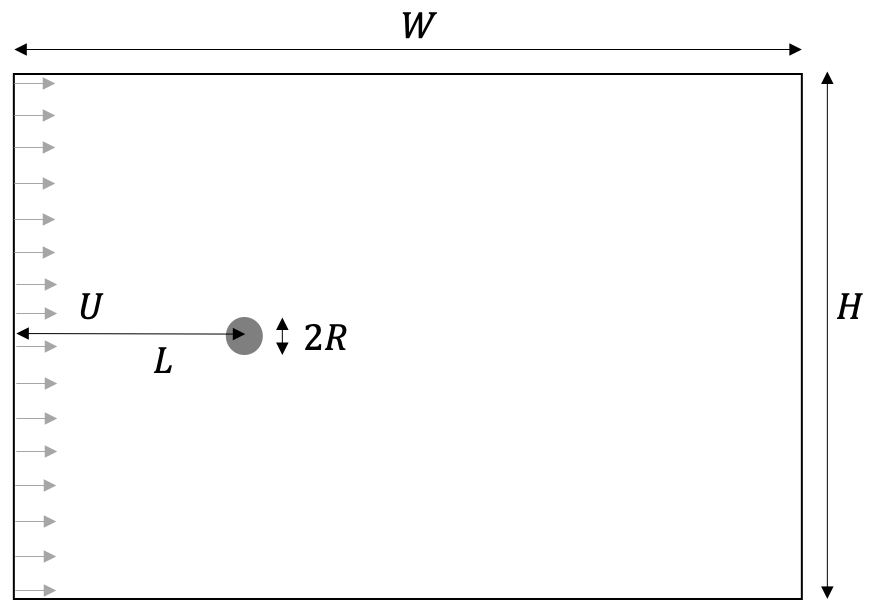
\includegraphics[width=0.5\linewidth]{figs/pf_geometry.png}
\caption{Problem set-up for flow over a cylinder in a rectangular enclosure.}
\label{fig:pf_geometry}
\end{figure}

This particular problem is selected to verify the Euler model because many other canonical Euler flows contain shocks that are not accurately captured with the numerical discretization described in Chapter \ref{sec:ph} due to a lack of ``shock-capturing'' terms \cite{hughes_1986,tezduyar_1986}. In addition, an analytic incompressible potential flow exists for comparison at low Mach numbers where compressibility effects\mdash the only underlying difference between a compressible Euler model and an incompressible potential flow model for the problem in Fig.\ \ref{fig:pf_geometry}\mdash are small. After outlining the potential flow solution, comparisons are made between Pronghorn's compressible Euler model and the incompressible potential flow solution for several different Mach numbers to illustrate that the compressible Euler solution tends towards the analytic incompressible solution as compressibility effects diminish.

The potential flow equations are a simplification to the Euler model for irrotational flow, or flows with zero vorticity \cite{munson,hirsch}. Irrotational flow is automatically satisfied if the velocity can be expressed as the gradient of a scalar potential \(\phi\),

\beq
\label{eq:PotentialVelocity}
\vec{V}=\nabla\phi\ ,
\eeq

\noindent because the curl of a gradient of a scalar is zero. For steady flow, substituting Eq. \eqref{eq:PotentialVelocity} into the incompressible Euler mass conservation equation gives a Laplace equation for the potential,

\beq
\label{eq:LaplacePhi}
\nabla^2\phi=0\ .
\eeq

\noindent For flow past a 2-D cylinder, an analytic solution to Eq. \eqref{eq:LaplacePhi} is formed by superimposing the solution for uniform inflow with the solution for a doublet, a combination of a source and sink of equal strength separated by a finite distance. A derivation of this solution is available in many introductory fluid mechanics texts \cite{munson}. For a cylinder centered on the origin, the \(x\)- and \(y\)-velocity components are

\beq
\label{eq:V1Analytic}
V_{x,p}=U\left\lbrack1-R^2\frac{x^2-y^2}{(x^2+y^2)^2}\right\rbrack\ ,
\eeq

\beq
\label{eq:V2Analytic}
V_{y,p}=-2UR^2\frac{xy}{(x^2+y^2)^2}\ ,
\eeq

\noindent where a \(p\) subscript is used to denote the potential flow solution. The Bernoulli equation is a simplification of the Euler momentum conservation equation for steady, irrotational, and isentropic flow. Because the \glspl{ic} are uniform, the potential flow model corresponds to isentropic flow. The Bernoulli equation for \(\vec{g}=\vec{0}\) is

\beq
\label{eq:B1}
\nabla\left(\frac{1}{2}V_iV_i+\frac{P}{\rho_f}\right)=0\ .
\eeq

\noindent To obtain the solution for pressure, apply Eq. \eqref{eq:B1} at the free-stream conditions of \(\vec{V}=U\vec{e}_x\) and \(P=P_\infty\) in combination with the velocity solutions in Eqs. \eqref{eq:V1Analytic} and \eqref{eq:V2Analytic} to give

\beq
\label{eq:PPressure}
P_p=P_\infty+\frac{1}{2}\rho_f\left(U^2-V_iV_i\right)\ .
\eeq

\begin{comment}
\noindent The surface pressure coefficient \(C_P\) represents a normalized pressure and is defined as

\beq
\label{eq:CPDef}
C_P\equiv\frac{P_\text{surface}-P_\infty}{\frac{1}{2}\rho_fU^2}\ .
\eeq

\noindent Substituting the pressure distribution in Eq. \eqref{eq:PPressure} with \(x^2+y^2=R^2\) into Eq. \eqref{eq:CPDef} gives the surface pressure coefficient for the potential flow as

\beq
\label{eq:PressureCoefficient}
C_{P,p}=1-4\sin^2(\theta)\ ,
\eeq

\noindent where \(\theta\) is the angle relative to the front of the cylinder. 
\end{comment}

\noindent Eqs. \eqref{eq:V1Analytic}, \eqref{eq:V2Analytic}, and \eqref{eq:PPressure}, are referred to here as the ``potential flow solution.''

The Mach number \(Ma\) is defined as

\beq
\label{eq:MaDef}
Ma\equiv\frac{\|\vec{V}\|}{c}\ 
\eeq

\noindent and represents the proximity of the flow to supersonic conditions. By writing the stagnation pressure as a Taylor series in terms of the Mach number for an ideal gas, compressibility effects are small for Mach numbers less than about 0.3. Therefore, in the limit of zero Mach number, Pronghorn's compressible Euler solution should predict velocities and pressures that match the potential flow solution. However, a flow simulation at exactly zero Mach number would correspond to a stagnant fluid for which matching the nonzero velocities in Eqs. \eqref{eq:V1Analytic} and \eqref{eq:V2Analytic} would not be possible. Therefore, the objective of comparing the compressible Euler solution with the incompressible potential flow solution is only to show that the difference between the two solutions decreases as the Mach number decreases. This investigation the verifies both 1)~correct numerical implementation of the inviscid form of the Navier-Stokes macroscale model and 2)~the mechanically compressible dependence on the fluid \gls{eos}.

Three different values of the Mach number are considered\mdash 0.08, 0.16, and 0.32. Each Mach number is a factor of two larger than the next-smallest value, and a Mach number of 0.32 is just above the classically-quoted value of 0.3 below which compressibility effects are insignificant.

A number of different metrics are used to assess the difference between the compressible Euler and incompressible potential flow solutions. The relative L$^2$ norm of the $x$-velocity, $y$-velocity, and pressure are evaluated over the entire domain and are represented as \(\|V_x-V_{x,p}\|/\|V_{x,p}\|\), \(\|V_y-V_{y,p}\|/\|V_{y,p}\|\), and \(\|P-P_p\|/\|P_p\|\), respectively. From Eqs. \eqref{eq:V1Analytic} and \eqref{eq:V2Analytic}, the potential flow velocity at the top of the cylinder is \(2U\). While the three norms listed earlier are computed over the entire domain, a point indicator of the velocity difference is useful for assessing error contributions due to the finite geometry. Therefore, the relative difference in the velocity at the top of the cylinder is included and represented as \(|V_x(0, R)-2U|/2U\).

A mesh refinement study is performed for the largest Mach number of 0.32 in the same fashion as in Section \ref{sec:natural_convection}. A starting mesh is uniformly refined until the relative change in the three L$^2$ norms described in the preceding paragraph is less than 5\% between two successive meshes. The finer of these two meshes is then used for all other Mach numbers.

First, a quantitative comparison between Pronghorn's compressible Euler model and the incompressible potential flow solution is provided. Table \ref{table:MNerror} summarizes the difference between the two models as a function of the Mach number. As expected, the difference between Pronghorn's compressible Euler solution and the incompressible potential flow solution decreases as the Mach number decreases.

\begin{table}[!h]
\caption{Difference between Pronghorn's compressible Euler solution and the incompressible potential flow solution as a function of the Mach number.}
\centering
\begin{tabular}{|c |c c c c|}
\hline\hline
\(Ma\) & \(\|V_x-V_{x,p}\|/\|V_{x,p}\|\) & \(\|V_y-V_{y,p}\|/\|V_{y,p}\|\) & \(|V_{x}(0, R)-2U|/2U\) & \(\|P-P_p\|/\|P_p\|\)\Tstrut\Bstrut\\
\hline
0.08 & \(3.53\times10^{-3}\) & \(3.27\times10^{-2}\) & \(2.62\times10^{-3}\) & \(1.50\times10^{-5}\)\Tstrut\\
0.16 & \(3.60\times10^{-3}\) & \(3.70\times10^{-2}\) & \(1.91\times10^{-2}\) & \(7.29\times10^{-5}\)\\
0.32 & \(4.88\times10^{-3}\) & \(8.48\times10^{-2}\) & \(8.72\times10^{-2}\) & \(6.71\times10^{-4}\)\Bstrut\\
\hline
\end{tabular}
\label{table:MNerror}
\end{table}

For the L$^2$ norms computed over the entire domain, or the second, third, and fifth columns in Table \ref{table:MNerror}, the reduction in these norms when halving the Mach number from 0.32 to 0.16 is much larger than the reduction when halving the Mach number from 0.16 to 0.08. For instance, the relative \(x\)-velocity norm decreases by a factor of 1.35 when halving the Mach number from 0.32 to 0.16, while only decreasing by a factor of 1.02 when halving the Mach number from 0.16 to 0.08. This occurs because of the finite size of the domain. That is, the difference in the two solutions should not be expected to tend to zero in the limit of zero Mach number\mdash the top and bottom walls are streamlines in the compressible Euler model, while the potential flow solution was derived with free stream \glspl{bc} as \(x, y\rightarrow\infty\) that result in nonzero curvature at \(y=\pm H/2\). To more clearly see this effect, consider the pointwise difference in the $x$-velocity at the top of the cylinder, which is sufficiently far from boundaries as to be unaffected by the \(W\) and \(H\) dimensions. In halving the Mach number from 0.32 to 0.16 and from 0.16 to 0.08, the relative difference in the $x$-velocity at the top of the cylinder decreases by a factor of 4.56 and 7.29, respectively. No significantly reduced solution difference is observed as the Mach number decreases for this pointwise metric.

The implicit \gls{bc} on the upper boundary does not impose any free-stream pressure such that the relative difference in the pressure distributions is comparatively unaffected by the finite nature of the domain. The relative difference in the pressure decreases by a factor of 9.20 as the Mach number is halved from 0.32 to 0.16 and by a factor of 4.79 as the Mach number is halved from 0.16 to 0.08.

To conclude this section, Pronghorn predicted velocity and pressure distributions for an inlet Mach number of 0.08 are presented. Define a nondimensional speed \(V^+\) as

\begin{equation}
V^+=\frac{\|\vec{V}\|}{U}\ .
\end{equation}

\noindent For the incompressible potential flow solution, \(V^+\) varies from zero on the front and back sides of the cylinder to 2.0 at the top and bottom of the cylinder. In the region near the cylinder, Fig.\ \ref{fig:Ma08} shows the nondimensional speed and pressure. In the speed subfigure, streamlines are shown as black lines. In the pressure subfigure, contours are shown colored by the pressure. The flow is nearly symmetric about the cylinder. At the front and rear stagnation points, the pressure is highest and the velocity lowest. Flow acceleration around the cylinder results in the highest velocities and lowest pressures occurring on the top and bottom of the cylinder. As already shown by the various norms in Table \ref{table:MNerror}, the velocity and pressure match the incompressible potential flow solution to within 4\% relative difference.

\begin{figure}[!h]
  \centering
  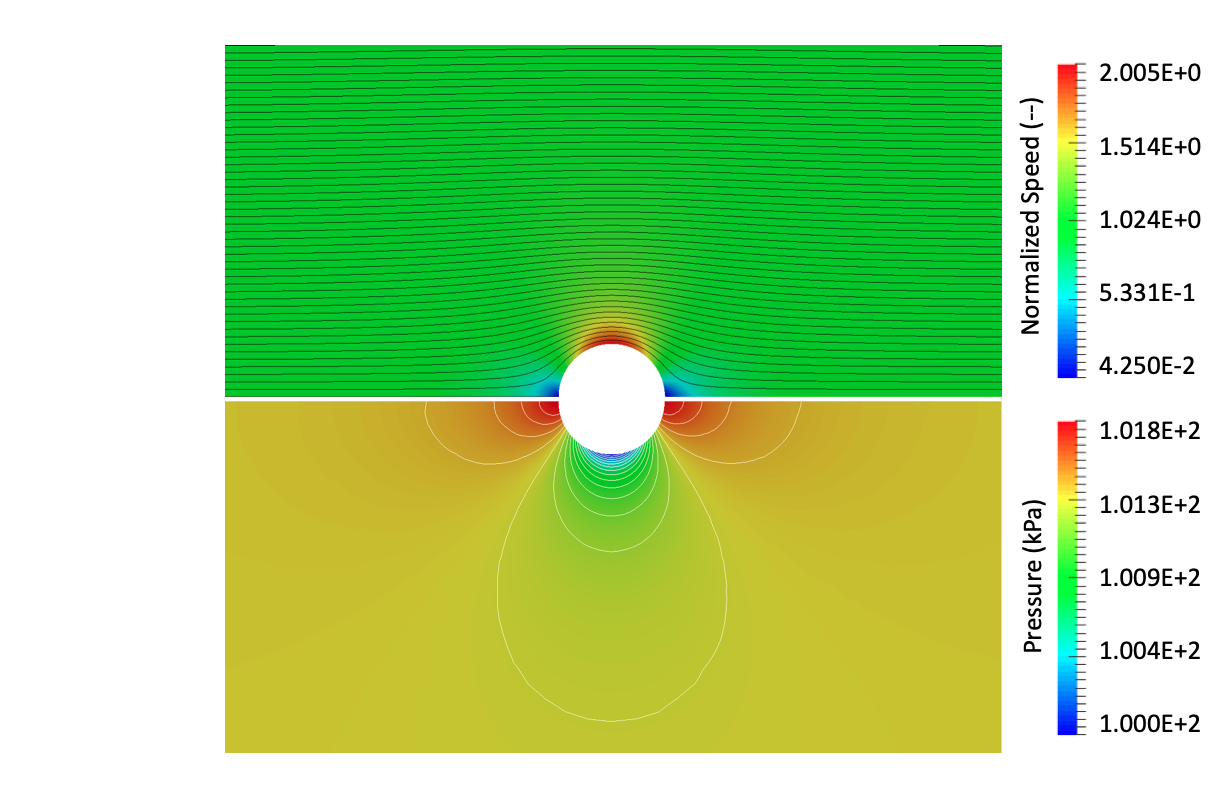
\includegraphics[width=0.7\linewidth]{figs/pf_Ma08.png}
  \caption{Pronghorn predicted \(V^+\), with streamlines in black, and \(P\), with contours shown colored by \(P\), for an inlet Mach number of 0.08.}
  \label{fig:Ma08}
\end{figure}

Overall, the mechanical compressibility effects are correctly modeled with the inviscid Navier-Stokes macroscale model. The combination of 1)~reduced differences between the compressible Euler and incompressible potential flow solutions as the Mach number decreases and 2)~low relative differences for Mach numbers in the range of \(0.08\leq Ma\leq0.32\) demonstrates the capacity of the inviscid Navier-Stokes model to simulate open flows, providing important verification for the modeling of high-Reynolds number flows in \glspl{pbr}.

\section{The Heat Source Decomposition Model}
\label{sec:verification_meso}

Given the computing resources available for routine design and analysis, the heterogeneous nature of \gls{pbr} fuels requires the use of multiscale models to predict temperatures. Simply homogenizing the fission heat source and thermal properties fails to capture the thermal resistance imposed by the low-conductivity buffer layer, and may result in significant underprediction of fuel temperatures. 

Two multiscale models were introduced in Chapter \ref{sec:PhysicalModels}\mdash the \gls{hsd} model and the \gls{hl} model. This section applies the \gls{hsd} model to a Cartesian domain consisting of nine \glspl{cfp} in a matrix and provides a comparison against a fully-resolved heat conduction solution of the same geometry. The objectives of this analysis are to 1)~verify the \gls{hsd} method for a simple, but representative, domain; 2)~explain the microscale ``translation'' process in Eq. \eqref{eq:MultiscaleSolution}; and 3)~address the accuracy of the averaging approximation in Eq. \eqref{eq:AvgT}. Because the \gls{mms} tests described in Section \ref{sec:mms} verify correct implementation of the diffusion kernels needed for the multi-layer \gls{hl} method, no such dedicated verification is required for the \gls{hl} method, which is simply a multi-layer conduction model.

For this demonstration problem, each \gls{cfp} is composed of five material layers with a uniform heat source of \(2\times10^8\) \si{\watt\per\cubic\meter} in the center kernel. While this power density is higher than that used in most \glspl{pbr}, the larger magnitude is selected to accentuate the differences between the meso and micro scale solutions. The \glspl{cfp} occupy 40\% by volume of the matrix material. Fig.\ \ref{fig:nine_particle_mesha} shows the mesh, colored by material ID, used to obtain the reference temperature solution. The \gls{cfp} layer thicknesses are the same as those in the \gls{pbfhr} design in Table \ref{table:pebble_props} and are typical of most \gls{triso} particle designs. Thermal properties in dimensionally consistent units are shown for each material in Fig.\ \ref{fig:nine_particle_mesha}. Thermal \glspl{bc} are selected in an arbitrary, but non-uniform, manner. The top, left, and right boundaries are set to 1100\si{\celsius}, 1100\si{\celsius}, and 1150\si{\celsius}, respectively, while the bottom boundary is insulated.

\begin{figure}[!h]
\centering
\hspace{1cm}
  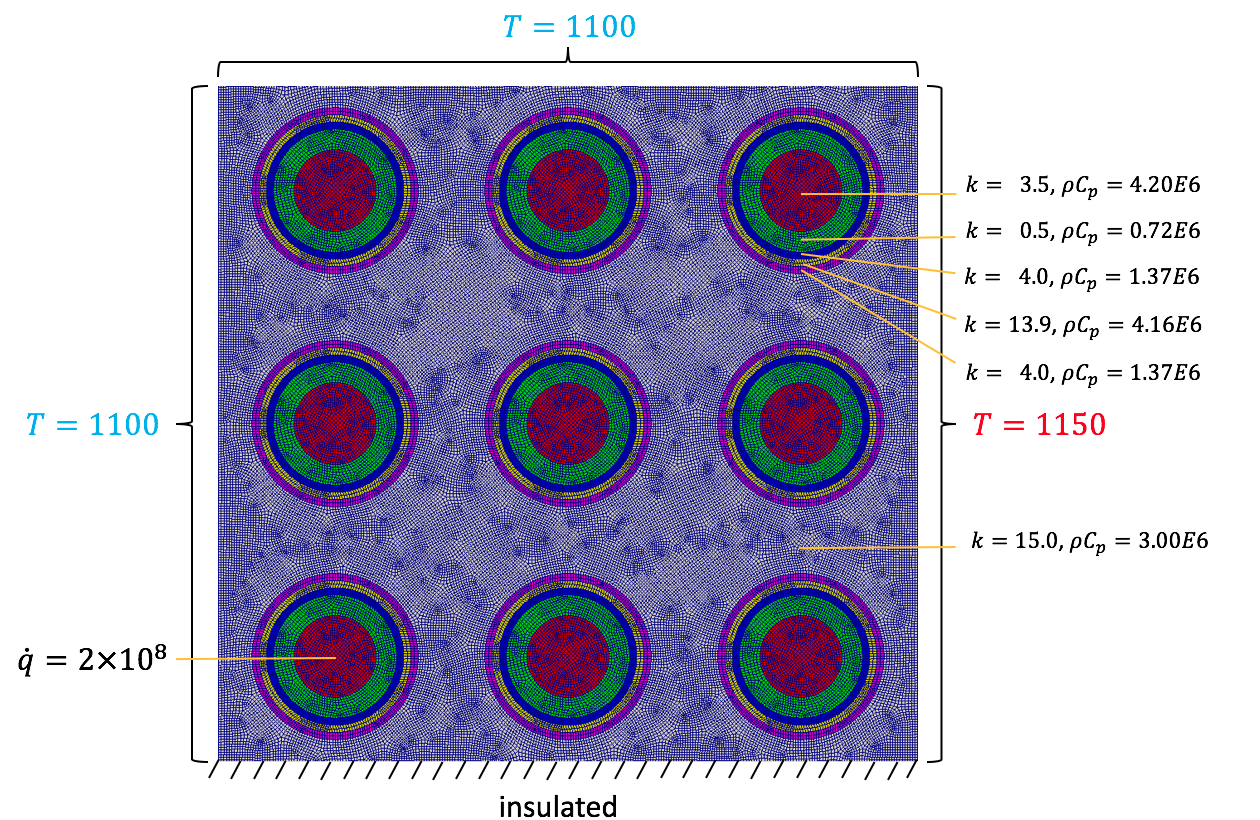
\includegraphics[width=0.75\linewidth]{figs/multiscale_9_problem.png}
\caption{Reference mesh and problem setup for a heterogeneous solid with \glspl{cfp} in a matrix.}
\label{fig:nine_particle_mesha}
\end{figure}

The reference temperature solution, shown in Fig.\ \ref{fig:nine_particle_mesh}, is obtained by solving the heat conduction equation in Eq. \eqref{eq:oem} with the \gls{moose} heat conduction module. The temperature contours are tightly packed in the second material layer in each \gls{cfp} due to its relatively low thermal conductivity. The objective of the \gls{hsd} model is to approximate the temperature distribution in Fig.\ \ref{fig:nine_particle_mesh} with significantly lower computational effort.

\begin{figure}[!h]
  \centering
  \hspace{3.2cm}
  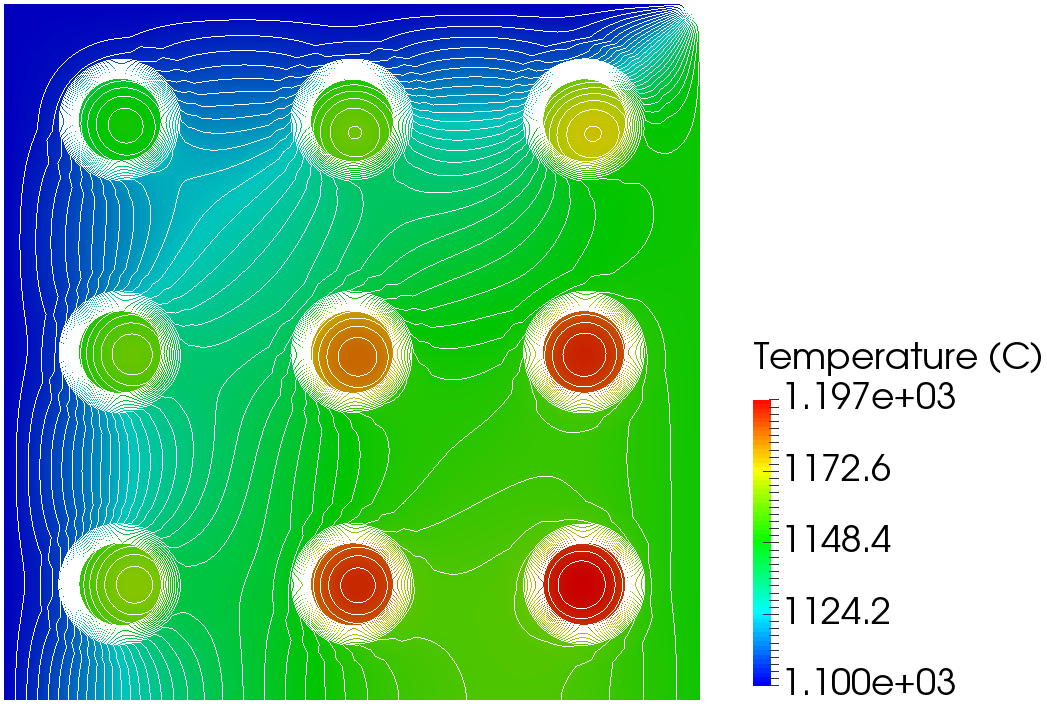
\includegraphics[width=0.63\linewidth]{../../pronghorn/doc/papers/MC2019/figures/compact_9_reference.png}
\caption{Reference temperature solution for the mesh in Fig.\ \ref{fig:nine_particle_mesha} with contour lines in white.}
\label{fig:nine_particle_mesh}
\end{figure}

The \gls{hsd} method involves the coupled solutions of the mesoscale model in Eq. \eqref{eq:MesoscaleSolution} and the microscale model in Eq. \eqref{eq:MicroscaleSolution}. The mesoscale mesh encompasses the entire heterogeneous region and is shown in Fig.\ \ref{fig:nine_particle_mesoscalea}. The \gls{cfp} properties are homogenized with the volume average in Eq. \eqref{eq:series}. \(\rho_\text{meso}\), and \(C_{p,\text{meso}}\) are then evaluated with the volume average in Eq. \eqref{eq:series}, while \(k_\text{meso}\) is evaluated with the Chiew and Glandt averaging theorem in Eq. \eqref{eq:ChiewGlandt}. The volumetric heat source is averaged over the \glspl{cfp} and matrix.

The mesoscale solution is shown in Fig.\ \ref{fig:nine_particle_mesoscaleb}. The mesoscale temperature represents a long-wavelength ``background'' response to the \glspl{bc}, averaged thermal properties, and averaged heat source. Note that the color bar in Fig.\ \ref{fig:nine_particle_mesoscaleb} is intentionally not the same as in Fig.\ \ref{fig:nine_particle_mesh} to reinforce that it is the sum of the meso and micro scale solutions that satisfies the imposed \glspl{bc}.

\begin{figure}[!h]
\centering
\begin{subfigure}{.45\textwidth}
  \centering
  
\includegraphics[height=0.72\linewidth]{../../pronghorn/doc/papers/MC2019/figures/mesoscale_9_mesh.png}
  \caption{Mesoscale problem}
  \label{fig:nine_particle_mesoscalea}
\end{subfigure}
\begin{subfigure}{.45\textwidth}
  \centering
  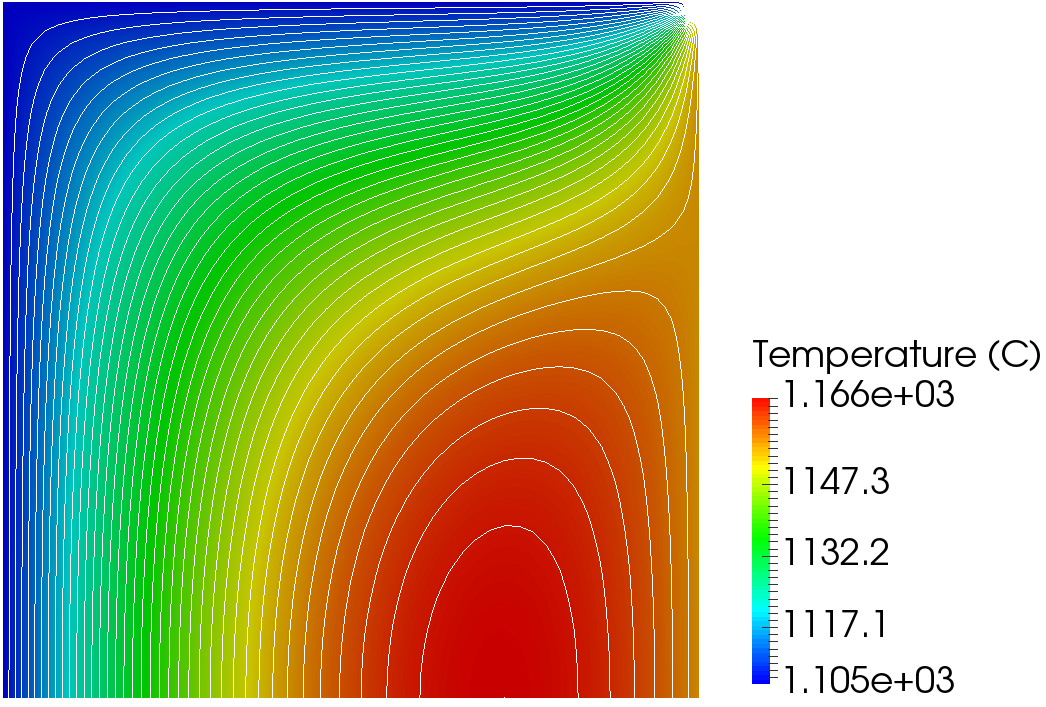
\includegraphics[height=0.71\linewidth]{../../pronghorn/doc/papers/MC2019/figures/compact_9_mesoscale.png}
  \caption{Mesoscale solution}
  \label{fig:nine_particle_mesoscaleb}
\end{subfigure}
\caption{\gls{hsd} mesoscale (a) mesh and (b) solution with contour lines in white.}
\label{fig:nine_particle_mesoscale}
\end{figure}

The microscale domain, shown in Fig.\ \ref{fig:micro_a}, is a 1-D representation of a \gls{cfp} plus a layer of matrix material sized to preserve all material \glspl{pf}. \(\rho_\text{micro}\), \(C_{p,\text{micro}}\), and \(k_\text{micro}\) are the local properties shown in Fig.\ \ref{fig:nine_particle_mesha}. The fluctuating heat source is positive within the central kernel and negative in all other regions to preserve the zero average. Fig.\ \ref{fig:micro_b} shows the microscale temperature solution. Because the fluctuating heat source is negative outside the central kernel, the temperature is negative in the outermost regions of the microscale domain.

\begin{figure}[!h]
\centering
\begin{subfigure}[b]{0.49\linewidth}
\centering
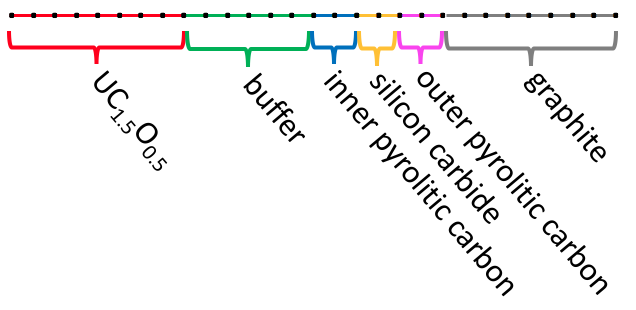
\includegraphics[width=6.cm]{../../pronghorn/doc/papers/MC2019/figures/microscale_domain_colored.png}
\vspace{2em}
\caption{Microscale problem}
\label{fig:micro_a}
\end{subfigure}
\begin{subfigure}[b]{0.49\linewidth}
\centering
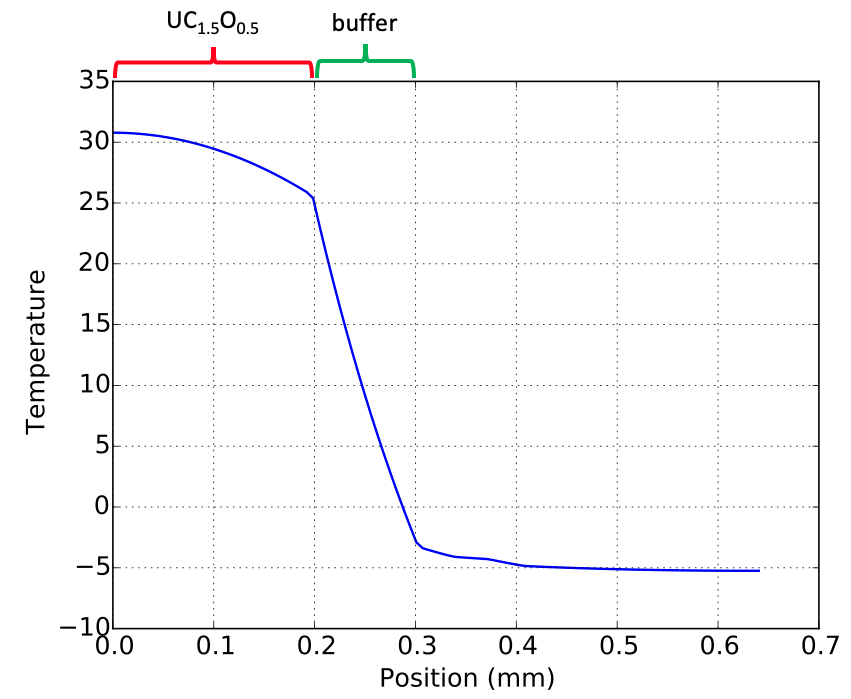
\includegraphics[height=6.cm]{../../pronghorn/doc/papers/MC2019/figures/microscale_solution.png}
\caption{Microscale solution}
\label{fig:micro_b}
\end{subfigure}
\caption{\gls{hsd} microscale (a) mesh and (b) solution.}
\end{figure}

Fig.\ \ref{fig:MMD_example} shows the reference and \gls{hsd} solutions along a horizontal line passing through the centers of the middle row of particles. The low-conductivity buffer results in significantly higher kernel temperatures than in surrounding materials. The bottom section of Fig.\ \ref{fig:MMD_example} shows the microscale solution translated to the location of each of the three particles. According to Eq. \eqref{eq:MultiscaleSolution}, the \gls{hsd} multiscale approximation is the sum of the long-wavelength mesoscale solution and the translated microscale solutions, and is shown as a red dashed line in Fig.\ \ref{fig:MMD_example}. The \gls{hsd} solution agrees very well with the reference temperature solution; the only source of error in the \gls{hsd} method is the homogenization of the mesoscale properties.

\begin{figure}[!h]
\centering
\includegraphics[width=0.6\linewidth]{../../pronghorn/doc/papers/MC2019/figures/nine_center_row_multiscale.png}
\caption{Multiscale, mesoscale, microscale, and reference solutions for the problem in Fig.\ \ref{fig:nine_particle_mesha}.}
\label{fig:MMD_example}
\end{figure}

It is important to note that legacy \gls{pbr} applications that simply homogenize the thermal properties and heat source to represent the fuel temperature with a single heat conduction \gls{pde} can only predict the long-wavelength background temperature in Fig.\ \ref{fig:MMD_example}. Such models would fail to capture the high kernel temperatures resulting from the buffer thermal resistance, and are hence not considered in this work.

Next, in order to verify applicability of the \gls{hsd} method to transients, consider the same problem in Fig.\ \ref{fig:nine_particle_mesha} with a time-dependent heat source given by

\begin{equation}
\label{eq:time_q}
\dot{q}=2\times10^8(t+1)\ .
\end{equation}

\noindent With this heat source, Fig.\ \ref{fig:time_q} shows the reference and \gls{hsd} multiscale solutions along a horizontal line passing through the centers of the middle row of particles. The \gls{hsd} approximation again agrees very well with the reference solution at all times considered. 

\begin{figure}[!h]
\centering
\begin{subfigure}[b]{0.49\linewidth}
\centering
\includegraphics[width=1.1\linewidth]{../../pronghorn/doc/figures/nine_particle_center_row_transient.png}
\caption{Solutions along line through center particles}
\label{fig:time_q}
\end{subfigure}
\begin{subfigure}[b]{0.49\linewidth}
\centering
\includegraphics[width=1.1\linewidth]{../../pronghorn/doc/figures/nine_particle_transient_postprocessors.png}
\caption{Solutions averaged in space}
\label{fig:avg_nine}
\end{subfigure}
\caption{Reference (---) and \gls{hsd} multiscale solutions (- -) (a) along a line through the centers of the middle row of particles and (b) spatially-averaged for the problem in Fig.\ \ref{fig:nine_particle_mesha} with the heat source in Eq. \eqref{eq:time_q}.}
\end{figure}

Fig.\ \ref{fig:avg_nine} shows the average temperatures of each material as a function of time. To reflect conditions typical of \gls{pbr} analysis, where the \gls{cfp} locations are unknown, the \gls{hsd} averages are evaluated with Eq. \eqref{eq:AvgT}. Excellent agreement is observed between the multiscale and reference solutions, especially considering that the mesoscale solution in this particular test problem varies on the order of the micro length scale.

The excellent agreement between the \gls{hsd} model and reference solution demonstrates the capacity of the \gls{hsd} model to simulate heat conduction in heterogeneous solids, providing important verification before application of the \gls{hsd} model to the Mark-1 \gls{pbfhr} in Chapter \ref{sec:pbfhr}.

\chapter{The SANA Experiments}
\label{sec:sana}

Power densities of gas-cooled \glspl{pbr} are typically low enough that radiation and conduction between touching pebbles, in combination with an ex-vessel cooling system, is sufficient to remove decay heat in a depressurized \gls{lofc} by natural convection cooling. However, low power densities result in larger reactor vessels that both complicate rail transport and increase structural material costs. Economic feasibility may motivate stretching paper design concepts to higher power densities or uprating an existing reactor. Safe reactor operation requires \gls{th} tools that can accurately model natural convection decay heat removal and the proximity of fuel temperatures to maximum allowable operating limits, especially when maximization of power density is a primary design objective. 

The SANA facility is a scaled experiment built and operated in Germany in the mid 1990s that models depressurized cool-down of gas-cooled \glspl{pbr} as a function of power density, coolant, and pebble properties \cite{SANA}. This section presents Pronghorn simulations of all steady-state and axisymmetric SANA experiments to assess the capability of the macroscale model for predicting core temperatures in depressurized \gls{lofc} events. This validation exercise is one piece of a much larger test matrix designed to qualify the multiscale model and its implementation in Pronghorn for gas- and liquid-cooled \glspl{pbr} \cite{ph_plan}.

The accuracy of porous media simulations is dependent on the closure relationships used to describe the solid-fluid phase distribution, interphase momentum and energy transfer, and lumped parameter effective heat transfer. Few \gls{th} simulations of reactor conditions have quantified the sensitivity of temperature predictions to the selection of particular closures from the enormous literature on the subject. For instance, a distillation of this literature over the course of a five year PhD project has resulted in the implementation of seven porosity models; four friction factor models; five interphase convective heat transfer coefficient models; 245 effective solid conductivity models as permutations of the seven \(\kappa_\text{radiation}\) models, seven \(\kappa_\text{conduction}\) models, and five \(\kappa_\text{contact}\) models; and two effective fluid conductivity models. The selection of these particular correlations for implementation in Pronghorn reflects their prominence in the porous media literature, and is by no means exhaustive. 

Due to the wealth of solid temperature data available, the SANA experiments are a useful baseline data set from which the sensitivity of pebble temperatures to variations in macroscale model closures can be obtained. By individually varying the porosity, near-wall effective solid thermal conductivity, interphase heat transfer and drag, and thermal dispersion models\mdash the five closures that tend to vary the most between applications of the macroscale model in Chapter \ref{sec:PhysicalModels} to gas-cooled \glspl{pbr}\mdash guidelines for closure selection and development are provided.

The remainder of this section is organized as follows. Section \ref{sec:experimental} introduces the SANA facility and experiments. Section \ref{sec:model} describes the Pronghorn model of the facility. Section \ref{sec:baseline} then presents simulation results for all 52 of the steady-state and axisymmetric experiments performed, plus an open upper plenum case, using a single set of baseline macroscale closures. When available, code-to-code comparisons are made to Flownex and GAMMA, two porous media applications that have previously been used to model gas-cooled \glspl{pbr} \cite{duToit2006,lim}. Simulation data has graciously been provided by Dr. C. G. Du Toit of the School of Mechanical and Nuclear Engineering at North-West University, South Africa and Dr. H. S. Lim of \gls{kaeri}.

In Section \ref{sec:sensitivity}, macroscale closures are individually varied from the baseline set used in Section \ref{sec:baseline} to determine the sensitivity of pebble temperature to closure selection. Finally, Section \ref{sec:5_summary} provides conclusions on the applicability of the friction-dominated macroscale model to the simulation of depressurized conduction cool-down in gas-cooled \glspl{pbr}, with particular emphasis on the importance of closure selection in future modeling activities and recommendations for experimental programs aimed at new closure development.

\section{The SANA Facility}
\label{sec:experimental}

The SANA facility consists of a closed cylindrical steel vessel containing about 9500 non-fueled pebbles heated by electrical resistance heaters in a variety of configurations in both steady and transient conditions \cite{SANA}. A depiction of the facility in a full-length, single-heater configuration is shown in Fig.\ \ref{fig:SANA_core}. Insulation on the bottom and top of the bed limits axial heat loss. The pebble surface temperature is measured throughout the bed with thermocouples at five different elevations, indicated as ``bottom,'' ``near bottom,'' ``middle,'' ``near top,'' and ``top'' in Fig.\ \ref{fig:SANA_core}. The precise axial coordinate of these measurement planes varied from test to test, and the scale shown in Fig.\ \ref{fig:SANA_core} is approximate. Most experiments involved a single centrally-located heater in an axisymmetric configuration, though several experiments placed multiple heaters throughout the bed so that the power distribution was no longer axisymmetric; these cases are not considered here.

\begin{figure}[h!]
\centering
\hspace{1.3cm}
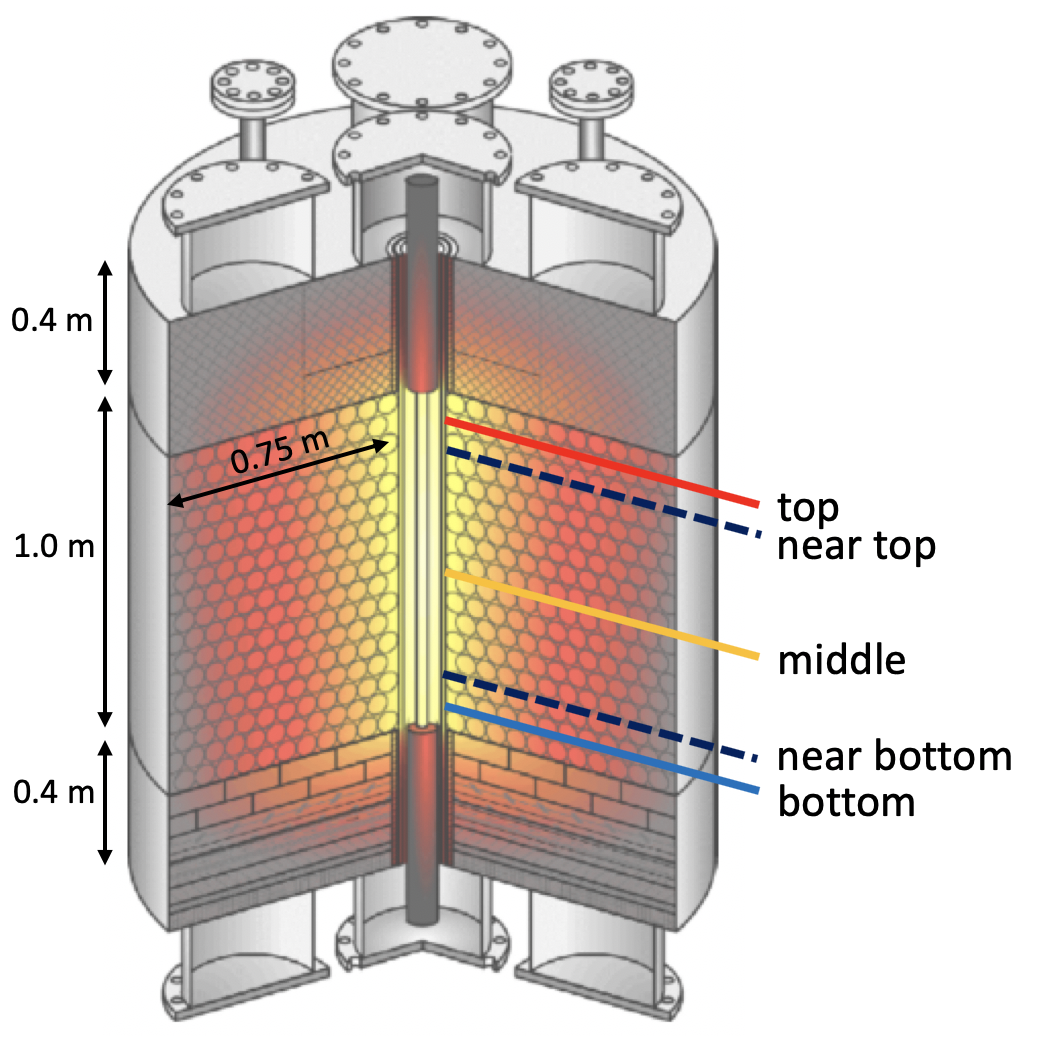
\includegraphics[width=0.5\linewidth]{figs/sana_core_labeled.png}
\caption{Illustration of the SANA facility with a single full-height heater. Temperature measurement planes are indicated as ``bottom,'' ``near bottom,'' ``middle,'' ``near top,'' and ``top'' (adapted from \cite{SANA}).}
\label{fig:SANA_core}
\end{figure}

A total of 52 steady-state and axisymmetric experiments were conducted with three different pebble designs, two different coolants, four different heater configurations, and seven different heater powers, resulting in a total of nearly 1300 solid temperature measurements. Fig.\ \ref{fig:sana_permutation} shows these experimental settings that, when permuted, encompass all the settings of the 52 experiments. Some heater configurations were only performed with 6 \si{\centi\meter} graphite pebbles, so not all experiments implied by Fig.\ \ref{fig:sana_permutation} were necessarily conducted, though all settings are represented.

The three pebble designs\mdash 6.5 \si{\centi\meter} diameter aluminum oxide, 6 \si{\centi\meter} diameter electric graphite, and 3 \si{\centi\meter} matrix graphite\mdash vary in their diameter and thermal properties. The smaller the pebble diameter, the greater the interphase friction and convective heat transfer. The three pebbles also have significantly different thermal conductivities; the electric graphite thermal conductivity is approximately two times and ten times larger than that of the matrix graphite and aluminum oxide, respectively. The higher the pebble thermal conductivity, the greater the effective solid thermal conductivity and heat transfer mechanisms independent of convection.

\begin{figure}[!h]
\centering
\includegraphics[width=0.9\linewidth]{figs/sana_permutation.png}
\caption{Experimental matrix for the 52 steady-state and axisymmetric SANA experiments (adapted from \cite{SANA}).}
\label{fig:sana_permutation}
\end{figure}

Experiments are performed with both helium and nitrogen due to the extensive use of helium coolant and nitrogen's thermodynamic similarity to air, barring high graphite corrosion rates. The SANA facility operates at atmospheric pressure, so both coolants correspond to depressurized \gls{lofc} conditions; experiments with nitrogen represent surrogates for air ingress, where natural convection cooling is distinct from that with helium. Helium and nitrogen have significantly different thermal properties; the helium thermal conductivity is approximately five times larger than that of nitrogen, resulting in stronger convective transport but weaker diffusive transport in nitrogen than in helium. The various combinations of pebble design and coolant result in different relative strengths of convective to diffusive transport and buoyant forces to friction losses. 

The partial length heater configurations are surrogates for partial control rod insertion, while the open plenum case models the bed-cavity interface found in most gas-cooled \glspl{pbr}. Finally, the various heater powers correspond to the decreasing decay heat levels at various times following an initial shutdown. The maximum power density of 28 \si{\kilo\watt\per\cubic\meter} represents about 1\% of the full power of a typical gas-cooled \gls{pbr} design, or decay heat levels several hours after shutdown.

All 52 of the steady-state and axisymmetric cases are simulated with Pronghorn. Validation results for eight cases are presented in detail, while the remaining 44 are summarized with error histogram plots. These eight cases are selected to cover most of the range of powers, heater arrangements, coolants, and pebble types used in the experiments, in addition to permitting direct comparison with the available Flownex and GAMMA results. Table \ref{table:CasesLetters} summarizes these eight cases and provides case letters for differentiation. One experiment with an open upper plenum is discussed as a separate demonstration of the macroscale model's capabilities for predicting bed-to-plenum heat and mass transfer. Fluid temperature and velocity results, for which no experimental data was collected, are also shown for a number of additional experiments aside from the eight highlighted cases.

\begin{table}[h!]
\caption{A summary of the SANA cases simulated with Pronghorn and presented in detail in this text. Case letters are provided for reference.}
\centering
\begin{tabular}{@{}cccccc@{}}
\toprule
\textbf{Case} & \textbf{Heater Description} & \textbf{Pebble Type} & \textbf{{\boldmath{\(d_p\)} (\si{\centi\meter})}} & \textbf{Fluid} & \textbf{Power (\si{\kilo\watt})}\\
\midrule
A & full-height & graphite & 6.0 & He & \color{white}0\color{black}5\\
B & full-height & graphite & 6.0 &He & 35\\
C & full-height & graphite & 6.0 & N & \color{white}0\color{black}5\\
D & full-height & graphite & 6.0 & N & 35\\
E & full-height & aluminum oxide & 6.5 & He & 30\\
F & full-height & aluminum oxide & 6.5 & N & 30\\
G & bottom half & graphite & 6.0 & He & 20\\
H & bottom half & graphite & 6.0 & N & 20\\
I & bottom half, open plenum & graphite & 6.0 & N & \color{white}0\color{black}5\\
\bottomrule
\end{tabular}
\label{table:CasesLetters}
\end{table}

\section{Computational Model}
\label{sec:model}

The low power and absence of forced convection cooling results in slow natural circulation flows with momentum conservation dominated by drag effects. Therefore, the friction-dominated model in Eq.\ \eqref{eq:PrimitiveEqns} is used for the macro length scale. The homogeneous pebble interiors and steady-state conditions preclude the need for meso and micro scale models because the temperature everywhere in a pebble with no heat source is equal to its uniform surface temperature. Helium and nitrogen properties are obtained with the \gls{sbtl} method described in Appendix \ref{sec:props}. Pebble properties are given in Appendix \ref{sec:props}.

The lack of significant azimuthal asymmetries justifies the use of a \gls{2d} cylindrically-symmetric geometry. For simplicity, only the interior of the vessel is modeled. That is, the left boundary coincides with the heater surface, the right boundary coincides with the inner surface of the vessel, and the bottom and top boundaries coincide with the inner surfaces of the insulation. The effects of the vessel and insulation on heat transfer are approximated using the thermal resistance concept\mdash the heat flux on a boundary is modeled as series conduction through a number of homogeneous layers, followed by parallel convection and radiation from the vessel surface to the ambient. That is, the boundary heat flux \(\tilde{q}\) is approximated as

\begin{equation}
\label{eq:ThermalResistanceBC}
\tilde{q}=\frac{T-T_\infty}{A_b\left\lbrack\sum_{i\ =\ 1}^{n_l}R_{\text{cond},i}+\frac{1}{\left(h_c+h_r\right)A_s}\right\rbrack}\ ,
\end{equation}

\noindent where \(A_b\) is the area of the boundary; \(A_s\) is the area of the surface; \(n_l\) is the number of conduction layers; \(R_{\text{cond},i}\) is the conduction resistance of the \(i\)-th layer; \(h_c\) is the convective heat transfer coefficient; and \(h_r\) is the radiation heat transfer coefficient,

\begin{equation}
\label{eq:RadiationHTC}
h_r=\varepsilon\sigma\left(T_\text{surf}^2+T_\infty^2\right)\left(T_\text{surf}^{\color{white}1\color{black}}+T_\infty\right)\ ,
\end{equation}

\noindent where \(T_\text{surf}\) is the surface temperature. In Eqs.\ \eqref{eq:ThermalResistanceBC} and \eqref{eq:RadiationHTC}, ``boundary'' refers to the mesh sideset where the \gls{bc} is applied and ``surface'' refers to the interface between the \mbox{\(n_l\)-th} conduction layer and the ambient. An under-relaxed fixed point iteration is performed to obtain \(T_\text{surf}\). Eq.\ \eqref{eq:ThermalResistanceBC} approximates the heat transfer through the conduction layers as unidirectional along \(\hat{n}\) and may not be accurate for very large thermal gradients in directions perpendicular to \(\hat{n}\).

On the bottom, top, and right boundaries, the heat flux applied to the solid energy conservation equation is given by Eq.\ \eqref{eq:ThermalResistanceBC} with constant insulation and vessel thermal properties \cite{SANA}. The vessel emissivity and convection heat transfer coefficient are assumed to be 0.8 and 15 \si{\watt\per\square\meter\per\kelvin}, respectively. Neither of these values are provided with the benchmark documentation, so both values were selected to be in the center of the ranges used by other participants \cite{rousseau,baggemann,becker2003,lim,tecdoc1163}. Due to the lower thermal conductivity of the fluid phase and the low velocities expected, the fluid is assumed insulated on the bottom, top, and right boundaries.

On the heater surface, the total heat flux \(\tilde{q}_\text{tot}\) is assumed uniform and is split between the phases according to the effective thermal conductivities \cite{alazmi}. On the left boundary, the heat flux into the solid phase is given as

\begin{equation}
\label{eq:HeatFluxSplitting}
\tilde{q}=\frac{\kappa_s}{\kappa_f+\kappa_s} \tilde{q}_\text{tot}\ ,
\end{equation}

\noindent while the heat flux into the fluid phase comprises the remainder of the total heat flux. Eq.\ \eqref{eq:HeatFluxSplitting} is a very crude approximation of the multi-phase heat transfer processes that occur near walls in packed beds. Other simplified \glspl{bc} have been proposed \cite{alazmi}, but preliminary tests with different \glspl{bc} did not show any clear advantage of any one option over another. Finally, zero normal mass flux is weakly imposed on all surfaces, while tangential slip is permitted. 

The baseline set of macroscale closures used in Section \ref{sec:baseline} are as follows. \(W\) is given by Eq.\ \eqref{eq:W_KTA}, \(\alpha\) is given by Eq.\ \eqref{eq:KTA}, and \(\kappa_f\) is given by Eq.\ \eqref{eq:KappaFluidBasic}. \(\kappa_s\) is given by the sum of Eqs.\ \eqref{eq:KappaRadiationBB}, \eqref{eq:KappaFluidConductionZS}, and \eqref{eq:KappaSolidConductionCT}, with Eq.\ \eqref{eq:Tsotsas} applied within a half pebble diameter of the walls as a correction to \(\kappa_\text{radiation}\). For all three pebble types, the emissivity, elastic modulus, and Poisson ratio are assumed to be 0.8, \(9\times10^9\) Pa, and 0.136, respectively\mdash values typically ascribed to \gls{pbr} fuel pebbles\mdash since more detailed information was not available. 

No information is available regarding the bed filling method, so \(\epsilon_\infty\) is selected as 0.39, a value commonly used for packed sphere beds. For all cases except the open plenum case, the porosity is given by Eq.\ \eqref{eq:ExpPorosity2} with \(\epsilon_\text{wall}=0.8\). For the open plenum case, the porosity in the plenum is unity and in the bed is given by Eq.\ \eqref{eq:ExpPorosity2} with \(\epsilon_\text{wall}=1\) to ensure a smooth transition to the plenum in the near-wall region.

Mesh refinement studies are performed for the highest-powered cases of each experiment category (such as nitrogen coolant with 3 \si{\centi\meter} pebbles and a long central heater) to ensure converged results, but for brevity are not shown here. Finally, to enable reproduction of the simulations presented in this chapter, Appendix \ref{sec:reproducibility} lists all data and input files related to this chapter.

\section{Baseline Results}
\label{sec:baseline}

This section presents Pronghorn simulations for the 52 steady-state and axisymmetric SANA experiments and one open plenum test using the baseline set of closures described at the end of Section \ref{sec:model}. 

Section \ref{sec:sana_subset} presents detailed validation results for the select cases given in Table \ref{table:CasesLetters}, while all 52 steady-state and axisymmetric cases are summarized in Section \ref{sec:AllTests}. To avoid repeating the same error discussion with each new validation case, all discussion of the effects of modeling simplifications and differences in the Pronghorn, Flownex, and GAMMA models is deferred to Section \ref{sec:AllTests}.

\subsection{A Selected Subset of the Experiments}
\label{sec:sana_subset}

A total of nearly 1300 solid temperature measurements were made across the steady-state and axisymmetric SANA experiments. While no fluid temperature or velocity data was recorded, a qualitative discussion of the effect of coolant and pebble properties on flow and heat transport via fluid temperature and velocity predictions provides useful physical intuition for understanding the later presentation of solid temperature data. Fig.\ \ref{fig:streamlines2} shows Pronghorn predictions of fluid temperature and velocity streamlines for the six experiments with a long central heater and 30 \si{\kilo\watt} heater power. The top and bottom rows show predictions for helium and nitrogen coolant, respectively. The left, middle, and right columns show predictions for 6 \si{\centi\meter} electric graphite pebbles, 3 \si{\centi\meter} matrix graphite pebbles, and 6.5 \si{\centi\meter} aluminum oxide pebbles, respectively. In each figure, the left axis is the $r$-$z$ symmetry axis that coincides with the center of the heater.

A natural convection flow is established as fluid buoyantly rises near the heater surface and cools near the vessel outer surface. The insulation on the bottom and top of the bed induces primarily radial temperature gradients. The low thermal conductivity of nitrogen results in more significant convective transport than in helium, which manifests as larger axial fluid temperature gradients and a recirculation vortex located closer to the bottom of the bed. 

The thermal conductivity of the pebbles is directly related to the maximum temperature in the bed\mdash from left to right, the pebble thermal conductivity decreases. Experiments with aluminum oxide pebbles and nitrogen coolant have the greatest convective heat transport, while experiments with graphite pebbles and helium coolant have the greatest diffusive heat transport. 

\begin{figure}[h!]
\centering
\centerline{
\includegraphics[height=0.55\linewidth]{figs/sana_30kW_vel.png}}
\caption{Pronghorn predicted fluid temperature and velocity streamlines for a full-length heater at 30 \si{\kilo\watt} for helium (top row) and nitrogen (bottom row) coolant for the three pebble types.}
\label{fig:streamlines2}
\end{figure}

To provide physical insight for the partial-length heater experiments, Fig.\ \ref{fig:streamlines1} shows Pronghorn predictions of fluid temperature and velocity streamlines for the eight experiments with a half-length heater in the bottom of the bed and 6 \si{\centi\meter} graphite pebbles. The top and bottom rows again show predictions for helium and nitrogen coolant, respectively, while each column corresponds to a unique power level. The higher the heater power, the further upward the recirculation vortex moves for the helium tests, as energy transfer is primarily diffusive and in the radial direction. For nitrogen, higher heater powers result in stronger fluid acceleration in the upwards direction, pushing the recirculation vortex further downwards as the fluid changes directions along the top and right walls of the vessel. Both of these observations are related to the stronger convective transport in nitrogen.

Moving to the solid temperature, similar trends with pebble and coolant thermal properties will be highlighted with each case. In presenting the validation data, all experimental results are shown as discrete points and Pronghorn predictions are shown as solid lines (---). When available, Flownex results are shown as dashed lines (- -) and GAMMA results are shown as dotted lines ($\ \cdots$). Measurements were taken at the five axial elevations shown in Fig.\ \ref{fig:SANA_core}, but only three of these elevations are plotted to simplify data presentation. The axial coordinate of these elevations is shown in the figure legends as $z=z_i$, where $z_i$ is the coordinate.

\begin{figure}[h!]
\centering
\centerline{
\includegraphics[height=0.6\linewidth]{figs/sana_bottom_vel.png}}
\caption{Pronghorn predicted fluid temperature and velocity streamlines for a partial-length heater in the bottom of the bed for helium (top row) and nitrogen (bottom row) for 6 \si{\centi\meter} graphite pebbles for four power levels.}
\label{fig:streamlines1}
\end{figure}

Figs. \ref{fig:helium_long} and \ref{fig:nitrogen_long} show Pronghorn and Flownex solid temperature predictions for heater powers of 5 and 35 \si{\kilo\watt} and 6 \si{\centi\meter} graphite pebbles with helium and nitrogen coolant, respectively. The 5 \si{\kilo\watt} cases in Figs. \ref{fig:helium_longa} and \ref{fig:nitrogen_longa} are shown on the same temperature scale of 0 to 500\si{\celsius}, while the 35 \si{\kilo\watt} cases in Figs. \ref{fig:helium_longb} and \ref{fig:nitrogen_longb} are shown on the same temperature scale of 0 to 1200\si{\celsius}. Similar to the fluid temperature shown in Fig.\ \ref{fig:streamlines2}, the greater diffusive transport in helium results in smaller axial solid temperature gradients and a lower maximum temperature as compared to nitrogen. Pronghorn and Flownex agree well for the helium cases and reasonably well for the nitrogen cases, though Pronghorn predicts lower temperatures at the lowest elevation in the nitrogen cases than Flownex. Both Pronghorn and Flownex tend to overpredict temperatures near the surface of the heater.

Fig.\ \ref{fig:long65} shows Pronghorn solid temperature predictions for a heater power of 30 \si{\kilo\watt} and 6.5 \si{\centi\meter} aluminum oxide pebbles with helium and nitrogen coolant. Compared to the graphite pebble experiments in Figs. \ref{fig:helium_long} and \ref{fig:nitrogen_long}, the lower thermal conductivity of the aluminum oxide results in larger radial temperature gradients and higher peak temperatures by about 400\si{\celsius}. Pronghorn predicts the experimental data well at all points except at the lowest elevation close to the heater surface for helium.

\begin{figure}[h!]
    \begin{subfigure}{0.5\linewidth}
        \centering
        \includegraphics[height=0.75\linewidth]{figs/exp_total_A.pdf}
       \caption{Case A: 5 \si{\kilo\watt} helium}
       \label{fig:helium_longa}
    \end{subfigure}
    \begin{subfigure}{0.5\linewidth}
        \centering
        \includegraphics[height=0.75\linewidth]{figs/exp_total_F.pdf}
        \caption{Case B: 35 \si{\kilo\watt} helium}
        \label{fig:helium_longb}
    \end{subfigure}
    \caption{Pronghorn (---) and Flownex (- -) predicted solid temperature for (a) case A and (b) case B, or a full-length heater with helium and 6 \si{\centi\meter} graphite pebbles.}
    \label{fig:helium_long}
\end{figure}

\begin{figure}[h!]
    \begin{subfigure}{0.5\linewidth}
        \centering
        \includegraphics[height=0.75\linewidth]{figs/exp_total_G.pdf}
       \caption{Case C: 5 \si{\kilo\watt} nitrogen}
       \label{fig:nitrogen_longa}
    \end{subfigure}
    \begin{subfigure}{0.5\linewidth}
        \centering
        \includegraphics[height=0.75\linewidth]{figs/exp_total_L.pdf}
        \caption{Case D: 35 \si{\kilo\watt} nitrogen}
        \label{fig:nitrogen_longb}
    \end{subfigure}
    \caption{Pronghorn (---) and Flownex (- -) predicted solid temperature for (a) case C and (b) case D, or a full-length heater with nitrogen and 6 \si{\centi\meter} graphite pebbles.}
    \label{fig:nitrogen_long}
\end{figure}

Fig.\ \ref{fig:bottom} shows Pronghorn, Flownex, and GAMMA solid temperature predictions for a heater power of 20 \si{\kilo\watt} in the bottom half of the bed with 6 \si{\centi\meter} graphite pebbles and helium or nitrogen coolant. Near the heater surface, the temperature distribution is inverted relative to the long central heater cases in Figs. \ref{fig:helium_long} and \ref{fig:nitrogen_long}, being highest at the bottom of the bed. This occurs due to the absence of a heat source in the top of the bed. The lower thermal conductivity of nitrogen results in poorer radial heat transport than in helium, resulting in an opposite temperature trend near the bed periphery compared to helium. All codes show similar trends in Fig.\ \ref{fig:bottom}, but the absolute variation is larger than for the full-length heater results. Pronghorn tends to underpredict temperatures in the higher elevations relative to Flownex and GAMMA. 

\begin{figure}[h!]
    \begin{subfigure}{0.5\linewidth}
        \centering
        \includegraphics[height=0.75\linewidth]{figs/exp_total_D2.pdf}
       \caption{Case E: 30 \si{\kilo\watt} helium}
    \end{subfigure}
    \begin{subfigure}{0.5\linewidth}
        \centering
        \includegraphics[height=0.75\linewidth]{figs/exp_total_J2.pdf}
        \caption{Case F: 30 \si{\kilo\watt} nitrogen}
    \end{subfigure}
    \caption{Pronghorn (---) predicted solid temperature for (a) case E and (b) case F, or a full-length heater with helium or nitrogen and 6.5 \si{\centi\meter} aluminum oxide pebbles.}
    \label{fig:long65}
\end{figure}

\begin{figure}[h!]
    \begin{subfigure}{0.5\linewidth}
        \centering
        \includegraphics[height=0.75\linewidth]{figs/exp_total_U2.pdf}
       \caption{Case G: 20 \si{\kilo\watt} helium}
    \end{subfigure}
    \begin{subfigure}{0.5\linewidth}
        \centering
        \includegraphics[height=0.75\linewidth]{figs/exp_total_Y2.pdf}
        \caption{Case H: 20 \si{\kilo\watt} nitrogen}
    \end{subfigure}
    \caption{Pronghorn (---), Flownex (- -), and GAMMA (\(\cdots\)) predicted solid temperature for (a) case G and (b) case H, or a half-length heater in the bottom of the bed and 6 \si{\centi\meter} graphite pebbles.}
    \label{fig:bottom}
\end{figure}

Finally, Fig.\ \ref{fig:plenuma} shows Pronghorn solid temperature predictions for a heater power of 5 \si{\kilo\watt} in the bottom half of the bed and an open plenum in the top third of the bed for 6 \si{\centi\meter} graphite pebbles and nitrogen coolant. Reasonable agreement is obtained with the experimental data, though temperatures are slightly overpredicted near the heater surface at the middle and top elevations. 

Fig.\ \ref{fig:plenumb} shows the predicted fluid temperature with velocity streamlines. The transition from the pebble bed to the open plenum is clearly visible in the velocity streamlines. Fluid re-entering the porous region is pulled towards the high-porosity region near the wall where friction factors are lower. When combined with the significantly reduced friction in the open plenum relative to the bed, this results in primarily radial flow in the plenum.

\begin{figure}[h!]
    \begin{subfigure}{0.5\linewidth}
        \centering
        \includegraphics[height=0.75\linewidth]{figs/piecewise_A3.pdf}
       \caption{Solid temperature}
       \label{fig:plenuma}
    \end{subfigure}
        \begin{subfigure}{0.5\linewidth}
        \centering
        \includegraphics[height=0.75\linewidth]{figs/A3_streamlines.png}
       \caption{Velocity streamlines}
       \label{fig:plenumb}
    \end{subfigure}
    \caption{Pronghorn predicted (a) solid temperature and (b) fluid temperature with velocity streamlines for case I, or an open plenum and 6 \si{\centi\meter} graphite pebbles.}
    \label{fig:plenum}
\end{figure}

It should be noted that the use of a friction-dominated model in the plenum is not justified as it is in the pebble bed because there is a large mixing region. However, the lack of experimental data for the plenum region precludes directly assessing the accuracy of the plenum velocity and fluid temperature predictions. Additional validation is required for open plenum geometries, though the solution in the bed region agrees reasonably well with experimental data.

\subsection{All Steady-State Axisymmetric Tests}
\label{sec:AllTests}

This section summarizes the results for all 52 steady-state and axisymmetric experiments, with a total of 1292 experimental pebble temperature data points. For simplicity, the plenum test shown at the end of Section \ref{sec:sana_subset} is excluded from the histograms shown here and in Section \ref{sec:sensitivity}. The error relative to the experimental measurements, \(e_\text{num}\) is defined as

\begin{equation}
\label{eq:Error}
e_\text{num}\equiv T_{s}\left(\vec{x}_i\right)-T_{s,\text{exp},i}\ ,
\end{equation}

\noindent where \(T_s\left(\vec{x}_i\right)\) is the predicted solid temperature at position \(\vec{x}_i\) and \(T_{s,\text{exp},i}\) is the experimentally-measured solid temperature at position \(\vec{x}_i\). The maximum error is defined to occur at the data point with error furthest from zero, and may be either positive or negative. 

Fig.\ \ref{fig:histogram} shows a histogram of the error for all 52 cases with the available Flownex and GAMMA data. Significantly more cases were simulated with Pronghorn than with Flownex and GAMMA. To provide a fair comparison of the average error and standard deviation, Table \ref{table:stats} shows the mean, standard deviation \(\sigma\), and maximum error for all 52 cases simulated with Pronghorn, the six cases simulated with Flownex, and the four cases simulated with GAMMA. 

\begin{figure}[h!]
\centering
\includegraphics[width=0.6\linewidth]{figs/histogram_abs_error.pdf}
\caption{Histogram of solid temperature error for Pronghorn (52 cases), Flownex (six cases), and GAMMA (four cases).}
\label{fig:histogram}
\end{figure}

In each column, the number of points compared between the three tools are the same. When directly comparing Pronghorn to Flownex and GAMMA, Pronghorn predicts a slightly smaller mean error and lower standard deviation relative to both Flownex and GAMMA. Pronghorn predicts a significantly smaller maximum error for the Flownex cases, but a slightly larger error for the GAMMA cases. Given the cases simulated, the three codes are of comparable accuracy. 

\begin{table}[h!]
\centering
\begin{threeparttable}
\caption{The mean, standard deviation \(\sigma\), and maximum solid temperature error for the six Flownex cases, the four GAMMA cases, and all 52 cases. All units are \si{\celsius}.}
\begin{tabular}{@{}lcc c c c cc c c c c@{}}
\toprule
 & \multicolumn{3}{c}{Flownex cases\hspace{0.01cm}\tnote{1}} &\phantom{a}& \multicolumn{3}{c}{GAMMA cases\hspace{0.01cm}\tnote{2}} &\phantom{a}& \multicolumn{3}{c}{\color{white}${\rvert^\dagger}^\dagger$\color{black}All cases\color{white}${\rvert^\dagger}^\dagger$\color{black}}\\
\cmidrule{2-4} \cmidrule{6-8} \cmidrule{10-12}
 & \textbf{Mean} & {\boldmath\(\sigma\)} & \textbf{Max.} && \textbf{Mean} & {\boldmath\(\sigma\)} & \textbf{Max.} && \textbf{Mean} & {\boldmath\(\sigma\)} & \textbf{Max.}\\
\midrule
Flownex & \color{white}-\color{black}19.8 & 51.4 & \color{white}-\color{black}207.0 && --- & --- & --- && --- & --- & ---\\
GAMMA & --- & --- & --- && \color{white}-\color{black}4.3 & 50.9 & 147.5 && --- & --- & ---\\
Pronghorn & \color{white}0\color{black}-7.8 & 47.5 & -155.8 && -1.6 & 48.7 & 148.4 && 22.6 & 54.6 & 198.6\\
\bottomrule
\end{tabular}
\label{table:stats}
\begin{tablenotes}
\item[1] \small A, B, C, D, H, and the 20 \si{\kilo\watt} top half heater with 6 \si{\centi\meter} graphite pebbles and nitrogen.
\item[2] \small G, H, and the 30 \si{\kilo\watt} long heater with 6 \si{\centi\meter} graphite pebbles with helium and nitrogen.
\end{tablenotes}
\end{threeparttable}
\end{table}

It should be noted that the presentation of the error and standard deviation for the SANA cases should not be taken as an indication of the expected accuracy of the macroscale model for all applications. Rather, this condensed presentation is performed to provide a quantitative comparison against Flownex and GAMMA and to provide a rough sense of the accuracy of porous media \gls{th} simulations in friction-dominated flows such as \gls{lofc} decay heat removal.

The standard deviation for all simulation tools is similar, on the order of 50\si{\celsius}. The SANA experiments are a challenging benchmark because of the large thermal gradients near the heater and outer radial wall. Fig.\ \ref{fig:error_location} shows the error in the Pronghorn predictions as a function of distance from the radial and axial walls. Black dots represent individual data points, while larger red dots are the means of the data at each value of the independent variable, either the radial distance or the axial distance. 

The spread, or standard deviation, in the error decreases with distance from radial and axial walls. This is expected because of the isotropic assumptions made in the derivation of porous media closures from bed-averaged data. Additional contributors to near-wall errors include the use of simplified thermal resistance \glspl{bc} and momentum equations that permit slip, the latter of which results in an overprediction of the velocity near the wall and a corresponding overprediction of convective heat transfer and drag. Therefore, the large standard deviation of 50\si{\celsius} can be partially attributed to the significant fraction of experimental data points close to bounding walls. 

\begin{figure}[h!]
    \begin{subfigure}{0.5\linewidth}
        \centering
        \includegraphics[width=1.0\linewidth]{figs/error_radial.pdf}
       \caption{Error vs. distance from radial wall}
       \label{fig:error_locationa}
    \end{subfigure}
    \begin{subfigure}{0.5\linewidth}
        \centering
        \includegraphics[width=1.0\linewidth]{figs/error_axial.pdf}
        \caption{Error vs. distance from axial wall}
        \label{fig:error_locationb}
    \end{subfigure}
    \caption{Solid temperature error as a function of distance from (a) a radial wall (inner or outer), and (b) an axial wall (lower or upper). Each black dot is one data point. Each red dot is the mean error for the data at each value of the independent variable.}
    \label{fig:error_location}
\end{figure}

Fig.\ \ref{fig:error_locationa} shows that the mean error decreases with distance from the radial walls, while no such trend is clearly visible in Fig.\ \ref{fig:error_locationb} for the mean error as a function of distance from the axial walls. This supports the claim that the SANA experiments are a challenging benchmark due to the very large thermal gradients in the radial direction. No such decrease in average error exists for distances from the axial walls, which are insulated to the extent that thermal boundary effects are less significant but are still characterized by slip effects and anisotropic momentum and heat transfer. This suggests that 1)~the average error in Pronghorn simulations will be lower for systems with less significant thermal boundary layers; and 2)~more sophisticated heat flux \glspl{bc} can potentially reduce mean error in the near-wall regions. 

On average, Pronghorn overpredicts the solid temperature by 22.6\si{\celsius}. In addition to the identified near-wall error contributions of isotropic closures, slip, and simplified resistance \glspl{bc}, additional modeling approximations that may have affected the accuracy of the simulations include the constant vessel surface convection coefficient and emissivity and the constant pebble emissivity, elastic modulus, and Poisson ratio. In all cases shown in Section \ref{sec:baseline}, temperatures are generally overpredicted near the heater surface. This may indicate that the closures used for \(\kappa_s\) underpredict the effective thermal conductivity in this region or that the pebble emissivity is too low. Pebble emissivities of 0.9 and 0.85 have been used in other simulations of \glspl{pbr} \cite{tecdoc1163,tecdoc1694}. Therefore, a higher emissivity is not without precedent, but an emissivity of 0.8 is used for easier comparison to Flownex and GAMMA. 

Additional insight can be obtained when considering the error for different subsets of the experiments as summarized in Table \ref{table:subcases}. On average, Pronghorn predicts the helium cases with 16.6\si{\celsius} lower standard deviation than the nitrogen cases. The maximum error for the nitrogen cases is 31.9\si{\celsius} higher than for the helium cases. The greater convective transport in nitrogen is more difficult to capture with the friction-dominated model. 

\begin{table}[h!]
\caption{The mean, standard deviation, and maximum error for different subsets of the 52 steady-state and axisymmetric SANA cases.}
\centering
\begin{tabular}{@{}l c c c c @{}}
\toprule
 & \textbf{\# Cases} & \textbf{Mean (\si{\celsius})} & \textbf{\boldmath{\(\sigma\)} (\si{\celsius})} & \textbf{Max. (\si{\celsius})}\\
\midrule
All cases & 52 & 22.6 & 54.6 & \color{white}-\color{black}198.6\\
Helium coolant & 26 & 20.5 & 45.8 & \color{white}-\color{black}166.7\\
Nitrogen coolant & 26 & 24.8 & 62.4 & \color{white}-\color{black}198.6\\
3 \si{\centi\meter} matrix graphite pebbles & 12 & 44.2 & 48.7 & \color{white}-\color{black}198.6\\
6 \si{\centi\meter} electric graphite pebbles & 28 & \color{white}0\color{black}2.0 & 48.4 & -189.6\\
6.5 \si{\centi\meter} aluminum oxide pebbles & 12 & 45.8 & 55.8 & \color{white}-\color{black}181.3\\
Full-length heater & 36 & 30.5 & 52.7 & \color{white}-\color{black}198.6\\
Partial-length heater & 16 & \color{white}0\color{black}3.9 & 54.7 & -189.6\\
\bottomrule
\end{tabular}
\label{table:subcases}
\end{table}

Pronghorn predicts temperatures with the aluminum oxide pebbles with a standard deviation approximately 7.3\si{\celsius} higher than the two types of graphite pebbles. This may be attributed to the use of graphite emissivity, Young's modulus, and Poisson ratio for the aluminum oxide pebbles due to a lack of aluminum oxide data. 

The 6 \si{\centi\meter} graphite pebble cases are predicted with remarkably lower mean error than the other two types of pebbles. While this may be partially attributable to the fact that partial-length heater cases were only performed with the 6 \si{\centi\meter} graphite pebbles, this lower error may be related to the use of the \gls{kta} correlations for drag and heat transfer, which were developed based on experiments using 6 \si{\centi\meter} graphite pebbles. Lower errors for the 3 \si{\centi\meter} matrix graphite and 6.5 \si{\centi\meter} aluminum oxide pebbles might be obtained if using closures based on those specific pebble designs. Finally, a margin of 1\% in temperature, 2 \si{\centi\meter} in axial position, and 1 \si{\centi\meter} in radial position are the levels of uncertainty in the experimental measurements themselves \cite{becker2003}.

Overall, good agreement is obtained with both Flownex and GAMMA. Visual comparisons against THERMIX, TINTE, and TRIO-EF results available in the literature \cite{tecdoc1163} show good agreement with Pronghorn. Differences between Pronghorn, Flownex, and GAMMA exist because of the use of different closures, equation models, and \glspl{bc}. For example, neither Flownex nor GAMMA consider an axial dependence in the porosity, while Pronghorn considers a \gls{2d} \(r\)-\(z\) dependence. Flownex and GAMMA include a viscous stress term in the conservation of momentum equation, while Pronghorn permits slip. Flownex uses a constraint-style equation to represent heat transfer between pebbles, while Pronghorn and GAMMA combine the solid effective heat transfer term with the conservation of solid energy equation. Different vessel surface convection coefficients are used in all three applications.

Significant development efforts in all three applications are required to fully disentangle these simultaneous effects to identify the most significant contributors to the different temperature predictions. Simulations of a small subset of the SANA experiments with the compressible Navier-Stokes macroscale model suggest that temperatures may differ by up to 20 to 30\si{\celsius} in some regions of the bed, though not always in the direction of lower error \cite{schunert_phr}. A rigorous quantification of the effect of macroscale model differences between Pronghorn, Flownex, and GAMMA is an area of future work. 

\section{Sensitivity to Macroscale Closures}
\label{sec:sensitivity}

This section explores the sensitivity of pebble temperature to particular closures for porosity, the near-wall treatment for the solid effective thermal conductivity, interphase heat transfer and drag, and thermal dispersion. The geometric representation and \glspl{bc} described in Section \ref{sec:model} are unchanged.

Table \ref{table:stats_location} shows the mean, standard deviation, and maximum error for the baseline Pronghorn model in comparison to various closure modifications. The data in each row was obtained by simulating all 52 steady-state and axisymmetric cases with a single isolated change in macroscale closures from the baseline model described in Section \ref{sec:model}. For example, the entry labeled ``constant \(\epsilon\)'' represents simulation predictions with the porosity closure used in the baseline model replaced by the constant porosity model in Eq.\ \eqref{eq:ConstantEps} with all other closures fixed. ``Near-wall scaling \(\kappa_s\)'' represents predictions with a \(0.5\) multiplier on \(\kappa_\text{radiation}\) in the near-wall region instead of the Tsotsas correlation in Eq.\ \eqref{eq:Tsotsas}. ``Ergun \(W\)'' represents predictions with the Ergun interphase friction factor in Eq.\ \eqref{eq:Ergun} instead of the \gls{kta} correlation in Eq.\ \eqref{eq:W_KTA}. ``Gnielinski \(\alpha\)'' represents predictions with the Gnielinski interphase convective heat transfer coefficient in Eq.\ \eqref{eq:GnielinskiPebblebed} instead of the \gls{kta} correlation in Eq.\ \eqref{eq:KTA}. ``With dispersion'' represents predictions with the linear Peclet dispersion model in Eq.\ \eqref{eq:LinearPecletKappaFluid} instead of the zero-dispersion model in Eq.\ \eqref{eq:KappaFluidBasic}.

To quantify the significance of the lack of complete experimental facility information, simulations are also performed for two different constant values of the vessel convection coefficient and for two different values of the pebble emissivity. Results are presented in terms of the thermocouple locations within the bed to illustrate how the error varies as a function of position. The near-wall region is defined to occur within a half pebble diameter of the walls, while the bulk region constitutes all other points. 459 points lie in the near-wall region, while the remaining 833 are in the bulk.

\begin{table}[h!]
\caption{The mean, standard deviation \(\sigma\), and maximum solid temperature error for all 52 cases simulated with Pronghorn as a function of location within the bed for various closure modifications to the baseline model described in Section \ref{sec:model}. All units are \si{\celsius}.}
\centering
\centerline{
\begin{tabular}{@{}l c c c c c c c c c c c@{}}
\toprule
 & \multicolumn{3}{c}{\color{white}${\rvert^\dagger}^\dagger$\color{black}All\color{white}${\rvert^\dagger}^\dagger$\color{black}} & \phantom{a}& \multicolumn{3}{c}{Near-Wall} &\phantom{a}& \multicolumn{3}{c}{Bulk}\\
 \cmidrule{2-4} \cmidrule{6-8} \cmidrule{10-12}
 & \textbf{Mean} & {\boldmath\(\sigma\)} & \textbf{Max.} && \textbf{Mean} & {\boldmath\(\sigma\)} & \textbf{Max.} && \textbf{Mean} & {\boldmath\(\sigma\)} & \textbf{Max.}\\
\midrule
Baseline & 22.6 & 54.6 & \color{white}-\color{black}198.6 && 29.3 & 60.5 & \color{white}-\color{black}198.6 && 18.9 & 50.7 & 181.3\\
Constant \(\epsilon\) & 34.2 & 66.0 & \color{white}-\color{black}280.1 && 42.1 & 74.4 & \color{white}-\color{black}280.1 && 29.8 & 60.4 & 250.4\\
Near-wall scaling \(\kappa_s\) & 35.5 & 52.0 & \color{white}-\color{black}197.3 && 41.3 & 58.5 & \color{white}-\color{black}197.3 && 32.3 & 47.8 & 191.1\\
Ergun \(W\) & 21.1 & 54.4 & \color{white}-\color{black}211.6 && 27.2 & 59.7 & -197.8 && 17.7 & 50.9 & 211.6\\
Gnielinski \(\alpha\) & 22.0 & 54.9 & \color{white}-\color{black}211.1 && 28.2 & 60.3 & -196.3 && 18.6 & 51.4 & 211.1\\
With dispersion & 21.5 & 54.2 & \color{white}-\color{black}208.1 && 27.5 & 59.6 & \color{white}-\color{black}194.1 && 18.1 & 50.7 & 208.1\\
\(h_c=10\) \si{\watt\per\square\meter\per\kelvin} & 36.1 & 51.3 & \color{white}-\color{black}218.0 && 41.4 & 57.0 & \color{white}-\color{black}206.8 && 33.2 & 47.6 & 218.0\\
\(h_c=20\) \si{\watt\per\square\meter\per\kelvin} & 11.6 & 57.8 & -215.3 && 18.5 & 63.1 & -215.3 && \color{white}0\color{black}7.8 & 54.3 & 203.6\\
\(\varepsilon=0.7\) & 35.5 & 63.6 & \color{white}-\color{black}221.4 && 45.0 & 70.7 & \color{white}-\color{black}221.4 && 30.3 & 58.7 & 195.0\\
\(\varepsilon=0.9\) & \color{white}0\color{black}9.5 & 48.8 & -179.5 && 13.7 & 53.9 & -179.5 && \color{white}0\color{black}7.2 & 45.7 & 167.3\\
\bottomrule
\end{tabular}
}
\label{table:stats_location}
\end{table}

For all models in Table \ref{table:stats_location}, the mean error and standard deviation are both approximately 10\si{\celsius} higher in the near-wall region than in the bulk. This is expected due to the use of isotropic macroscale closures and the use of slip \glspl{bc}, and is in line with the dependence shown in Fig.\ \ref{fig:error_location}. Interestingly, the location of the maximum error is not wholly dominated by the near-wall region; of the 10 models considered, the highest error occurs in the bulk region for four models.

Less than 2\si{\celsius} difference in both the mean and standard deviation are observed when varying the drag, interphase heat transfer, and thermal dispersion models. This relative average insensitivity to the drag and heat transfer correlation agrees with results observed by others \cite{becker}. However, the maximum error for the Ergun drag model, the Gnielinski convective heat transfer model, and the linear Peclet thermal dispersion model result in 26.8 to 30.3\si{\celsius} higher maximum error in the bulk region, but little absolute change in the near-wall region. 

The solid temperature is sensitive to both the porosity model and the near-wall effective solid thermal conductivity treatment. A constant porosity on average results in a 11.6\si{\celsius} higher error and a 11.4\si{\celsius} higher standard deviation than a \gls{2d} porosity. The maximum error in the near-wall and bulk regions increases by 81.5\si{\celsius} and 69.1\si{\celsius}, respectively. A simple scaling factor applied to the effective solid thermal conductivity in the near-wall region results in a 12.9\si{\celsius} higher error, but a 2.6\si{\celsius} lower standard deviation, than the use of a different \(\kappa_\text{radiation}\) correlation. The maximum error in the near-wall region is relatively unaffected, while the maximum error in the bulk region increases by 9.8\si{\celsius}.

While a constant porosity only differs from the \gls{2d} \(r\)-\(z\) porosity in the near-wall region, and the wall treatment for solid effective thermal conductivity is only applied in the near-wall region, it is important to note that the use of these different closures affects the accuracy in all regions of the bed. Additional investigations are required to determine how these conclusions extend to geometries with larger bed to pebble diameter ratios. 

The solid temperature is also sensitive to the vessel convection coefficient and pebble emissivity. A range of 24.5\si{\celsius} in mean error and 6.5\si{\celsius} in standard deviation is observed depending on the selection of \(h_c\), while a range of 26.0\si{\celsius} in mean error and 14.8\si{\celsius} in standard deviation is observed depending on the selection of \(\varepsilon\). For all the variations in closure parameters, increasing the pebble emissivity from 0.8 to 0.9 is the only change that simultaneously results in a lower mean error, a smaller standard deviation, and a lower maximum error relative to the baseline model. This strong dependence on emissivity has been observed elsewhere, and motivates complete characterization of pebble material properties \cite{tecdoc1163}. Some error and spread in the Pronghorn simulations must therefore be attributed to a lack of complete experimental and material details in the benchmark specifications.

\section{Summary and Conclusions}
\label{sec:5_summary}

Essential to the development of any new simulation tool is the establishment of a strong validation base. This section demonstrated validation of the friction-dominated macroscale model and its numerical implementation in Pronghorn with the SANA experiments, a scaled experiment modeling depressurized natural convection decay heat removal. Using a single baseline set of closures, Pronghorn on average overpredicts solid temperature by 22.6\si{\celsius} with a standard deviation of 54.6\si{\celsius}. A code-to-code comparison with Flownex and GAMMA shows similar accuracy, but with the additional advantages of \gls{3d} unstructured meshing and comprehensive multiphysics coupling to \gls{moose} applications. 

The standard deviation decreases with distance from radial and axial walls, while the error only decreases with distance from radial walls. These observations highlight the need for anisotropic drag and heat transfer closures for near-wall regions, which are all but absent from the porous media literature. The primarily radial temperature gradient in the SANA facility also suggests that more accurate predictions can be achieved with improved isotropic closures such as heat flux \glspl{bc} and near-wall corrections to the effective solid thermal conductivity. 

Future computational and physical experiments must consider the near-wall region as distinct from the bulk region. Multiscale coupling to high-resolution \gls{cfd} or the incorporation of new experimentally-derived closures has the potential to reduce the standard deviation in near-wall regions and consequently achieve more precise predictions of \gls{pbr} \gls{th} to allow reactor design with smaller thermal margins and improved economic viability. The SANA experiments are particularly well-suited for a multiscale demonstration due to the relatively small vessel size and the high number of measurements taken within \(d_p/2\) distance from walls.

The standard deviation and maximum error are 16.6\si{\celsius} higher and 31.9\si{\celsius} higher, respectively, for the experiments with nitrogen coolant. The greater convective transport in nitrogen than in helium is more difficult to capture with the friction-dominated model. Future work will repeat the SANA experiments with the compressible Navier-Stokes model to determine the improvement in accuracy when considering momentum advection.

Interestingly, the error is about 40\si{\celsius} lower for the experiments with 6 \si{\centi\meter} diameter graphite pebbles than for the other two pebble types. While this may be partially attributable to the absence of partial-length heater tests with other pebbles, this lower error may also be due to the use of macroscale heat transfer and drag closures obtained specifically from experiments with 6 \si{\centi\meter} diameter graphite pebbles \cite{KTA,KTAhtc}. Further, the higher error associated with the aluminum oxide pebble experiments and the sensitivity to the vessel convection coefficient and pebble emissivity show that a potentially large systematic error term is present resulting from incomplete experimental characterization.

Statistical analysis shows that the interphase drag, heat transfer, and thermal dispersion models are, on average, of little significance to solid temperature, though errors in the bulk region of the bed increased by up to 30.3\si{\celsius} when using different closures. The solid temperature is sensitive to the models used for porosity and the near-wall treatment of the solid effective thermal conductivity in the entirety of the bed. The highest single increase in error of 81.5\si{\celsius} was observed when switching from a \gls{2d} porosity distribution to a constant distribution. Similar sensitivity studies should be repeated for more systems to generalize these conclusions as a function of power density, bed size, and other characteristic scales.


\chapter[The Pebble Bed Fluoride-Salt-Cooled High-Temperature Reactor]{The Pebble Bed Fluoride-Salt-Cooled High-Temperature Reactor}
\chaptermark{The Pebble Bed FHR}
\label{sec:pbfhr}

% I'd have an introductory sentence at the least that frames this chapter, potentially a paragraph. 
Throughout most of the history of the \gls{pbr} concept, helium has been the working fluid of choice \cite{claxton,hecker,oehme,nrc_avr,moormann,thtr_1990,hofmann,thomas,koster,gao,chen_htr,xu_htr,htrpm}. Helium has low neutron interaction cross sections, a thermal conductivity several times larger than other common gases \cite{gases_k}, and is chemically compatible with fuel and structural materials. 

In the past 20 years, considerable interest has grown in the use of molten salt coolants for \glspl{pbr}. The volumetric heat capacities of molten salts, like most liquids, are two to three orders of magnitude higher than those of gases at the same temperature and pressure. Even when pressurized to tens of atmospheres, the lower volumetric heat capacity of gas-cooled systems limits them to power densities two to three orders of magnitude smaller than liquid-cooled systems. Power density often directly translates to the structural material inventory, which contributes roughly 10\% of the overnight capital cost of construction \cite{xin_wang_thesis}. Atmospheric pressure systems also eliminate many complex pressurizing systems, further reducing cost.

The early development of gas-cooled systems emphasized high outlet temperatures needed for process heat applications. While the initial goal of a sustained 1000\si{\celsius} outlet temperature has in most gas-cooled designs been reduced to the 750\si{\celsius} range due to material limitations, the high boiling points of molten salts enable operation at similar temperatures as gas-cooled systems while retaining the operational simplicity associated with single-phase flow. High temperature operation also corresponds to higher thermal efficiency. 

To place these statements in a more quantitative perspective, Fig.\ \ref{fig:fluid_T_p} shows characteristic primary loop operating pressure and core outlet temperature for reactor designs based on five different coolants\mdash water in a \gls{bwr}, water in a \gls{pwr}, sodium in a fast reactor, carbon dioxide in an \gls{agr}, helium in a \gls{htgr}, \gls{flibe} in a \gls{htr}, and an organic oil in an organic-cooled reactor\hspace{0.01cm}\footnote{Water in a \gls{scwr} is not included because the extreme changes in thermal properties with temperature and pressure at and beyond the critical point make calculation of a meaningful average \(\rho_fC_{p,f}\) difficult.}. The area of each circle is proportional to the volumetric heat capacity \(\rho_fC_{pf}\) of each coolant at the average operating temperature and pressure. 

\begin{figure}[h!]
\centering
\includegraphics[width=0.6\linewidth]{figs/fluid_T_p.pdf}
\caption{Characteristic pressure and outlet temperature for reactor designs based on five common coolants. The area of each circle is proportional to \(\rho_fC_{p,f}\).}
\label{fig:fluid_T_p}
\end{figure}

Salt-cooled designs can operate at similar outlet temperatures as many helium-cooled \glspl{pbr} and carbon dioxide cooled \glspl{agr} without significant pressurization. Water coolants require significant pressurization to reach relatively low outlet temperatures with sufficient heat removal capabilities; to the author's knowledge, water coolants have only been proposed for a fluidized bed concept introduced in Chapter \ref{sec:intro} \cite{sefidvash,sefidvash_1996}.

Most chemically pure molten salts are compatible with common structural materials such as nickel alloys and graphite \cite{fratoni}. Lubrication of graphite in salt is also expected to result in significantly less graphite dust production from frictional pebble wear than in helium-cooled \glspl{pbr}. Further, many fission products are soluble in molten salts. Through proper fission product cold trap design, salt-cooled systems may exhibit a more predictable source term than gas systems, simplifying both accident analyses and decommissioning activities \cite{moormann}.

The selection of reactor coolant is always a balance between many design objectives that include efficiency, reliability, safety, and economics. Molten salts have relatively high freezing points, in the vicinity of 450 to 500\si{\celsius}; extensive trace heating systems are required to prevent salt freezing and flow blockages. And while salts such as \gls{flibe} contribute to neutron moderation \cite{fratoni}, the high \((n,^3\text{H})\) absorption cross section in $^6$Li requires enrichment of the lithium in lithium-bearing salts from a natural $^7$Li concentration of 92.41\% to high purities, typically 99.995\%, to ensure a negative coolant temperature coefficient and acceptable tritium production rates. The lack of significant infrastructure results in an uncertain cost associated with $^7$Li enrichment. The design of \gls{flibe}-cooled \glspl{pbr} in particular often includes additional constraints on minimizing coolant inventory to reduce cost \cite{pbfhr}.

The multiscale model described in Chapter \ref{sec:PhysicalModels} applies to all single-phase \glspl{pbr}. Chapter \ref{sec:sana} presented validation of the friction-dominated macroscale model to depressurized conduction cool-down in gas-cooled \glspl{pbr}. At the time of writing, a lack of experimental data for salt-cooled \glspl{pbr} precludes a similar validation for salt systems. Therefore, in lieu of validation exercises, this section demonstrates application of the multiscale model to full-core, steady-state analysis of a salt-cooled \gls{pbr} considering the pebble bed, outer reflector bypass, and conjugate heat transfer with structural materials. 

The objectives of this section are to 1)~assess the capability of the multiscale model for capturing physics important to salt-cooled \glspl{pbr}; 2)~describe the incorporation of high-resolution \gls{cfd} into the coarse-mesh multiscale model for closure generation; and 3)~predict the core \gls{th} of a salt-cooled design of current interest to the Nuclear Engineering department at \gls{ucb}\mdash the Mark-1 \gls{pbfhr}. 

This particular concept design is selected for application of the multiscale models developed in this dissertation because several aspects of the core design both highlight model and implementation strengths relative to ``legacy'' \gls{pbr} simulation tools and constitute significantly different \gls{th} conditions than seen in most helium-cooled \glspl{pbr}. For example, a combination of radial and axial inflow \glspl{bc} results in multi-dimensional core flow, rather than the ``plug'' flow typically observed in helium-cooled \glspl{pbr}. The interaction of these non-uniform flow \glspl{bc} with non-Cartesian inflow and outflow boundaries necessitates unstructured meshing capabilities. 

An unconventional reflector block design with strong coupling between horizontal and vertical flow channels requires generation of new drag closures with off-line \gls{cfd} modeling. The pebble design is also distinct from the gas-cooled design shown in Fig.\ \ref{fig:pbr_fuel}. A very thin fuel-matrix annulus, as opposed to a large central heterogeneous core, may cause the \gls{hl} method to perform poorly because of thermal resistance distortion. The \gls{hsd} verification performed for compacts in Chapter \ref{sec:vv} may also not extend to thin regions, especially when considering the ad hoc averaging and extrema approximations in Eqs. \eqref{eq:MaxT}--\eqref{eq:AvgT}.

This section also incorporates many additional physical phenomena that are often omitted in preliminary analyses of salt-cooled designs. In place of a simple volume average of the phase thermal conductivities \cite{xin_wang_thesis,scarlat}, inter-pebble stagnant conduction, contact conduction, and radiation are included. And while the increase in advective heat transfer due to thermal dispersion is usually neglected \cite{xin_wang_thesis,scarlat}, this ``braiding'' effect is considered. Likely more significant than the inclusion of additional macroscale physics is the addition of bypass flow modeling. A lack of reflector drag closures prevented earlier studies from accounting for the reduction in core cooling associated with core bypass, resulting in non-conservative maximum fuel temperature predictions.

The remainder of this section is organized as follows. Section \ref{sec:mark1} describes the Mark-1 \gls{pbfhr} design, revisiting in greater detail the features highlighted in the preceding paragraphs. Section \ref{sec:pbfhr_model} describes the computational model of the Mark-1 \gls{pbfhr} core. To determine the applicability of the \gls{hsd} and \gls{hl} methods to fuel designs with thin fuel-matrix annuli, Section \ref{sec:meso_fhr} compares the \gls{hsd} and \gls{hl} fuel models against reference, explicitly-resolved, \gls{pbfhr} pebbles. To enable full-core modeling incorporating bypass flow, Section \ref{sec:bypass} describes the generation of drag correlations for the outer reflector blocks at end-of-life using COMSOL Multiphysics. Several gap sizes are investigated to identify the sensitivity of core undercooling to reflector block lifetime. 

Section \ref{sec:core} then combines the macroscale model described in Section \ref{sec:macro_deriv}, the meso and micro scale models described in Section \ref{sec:mesomicro} and verified in Section \ref{sec:meso_fhr}, and the high-resolution reflector block closure generation discussed in Section \ref{sec:bypass} to full-core steady-state analysis of the Mark-1 \gls{pbfhr}. Section \ref{sec:inflow} evaluates several potential core-flow \glspl{bc} from the perspective of the bypass fraction, outlet fluid temperature distribution, and pumping power. For a number of different reflector block gap distributions, an inflow \gls{bc} design that achieves low bypass, pressure drop, and maximum outlet temperatures is recommended for more detailed analysis.

Section \ref{sec:depth} then provides predictions of pressure; velocity; and fuel, coolant, and structural material temperatures for the coupled pebble bed and reflector system with the inflow \gls{bc} developed in Section \ref{sec:inflow}. Finally, Section \ref{sec:conclusions_fhr} revisits the limitations of the present work and outlines next steps in improving multiscale models for salt-cooled \glspl{pbr}.

\section{The Mark-1 Design}
\label{sec:mark1}

The Mark-1 \gls{pbfhr} is a 236 MW$_\text{th}$ \gls{flibe}-cooled \gls{pbr} concept developed by \gls{ucb}, \gls{mit}, and \gls{uw} through a \gls{doe} \gls{irp} \cite{pbfhr}. The combination of a high boiling point and low vapor pressure coolant with a robust pebble fuel form enables high-temperature and atmospheric pressure operation with passive decay heat removal. This section introduces the reactor design features salient for multiscale \gls{th} analysis in Sections \ref{sec:meso_fhr}--\ref{sec:core}. All geometric, operational, and material descriptions of the \gls{pbfhr} are taken from a technical design report published in 2014 by the \gls{th} Lab at \gls{ucb} \cite{pbfhr}. For brevity, the ``Mark-1'' designation is dropped throughout this section.

The nominal operating conditions of the \gls{pbfhr} relevant to core thermal analysis are summarized in Table \ref{table:operating}. The core consists of fixed block-type inner and outer graphite reflectors that constrain the pebbles into an annulus. Fig.\ \ref{fig:pbfhr_core} shows an illustration of the pebble bed region and a crude representation of the inner reflector. Conceptual streamlines are hand-drawn as gray lines; flow into the outer reflector is not shown.

\begin{table}[htb!]
\caption{Nominal operating conditions of the \gls{pbfhr}.}
\centering
\small
\begin{tabular}{|l|c|}
\hline\hline
Operating Condition & Value\Tstrut\Bstrut\\
\hline
Thermal power & 236 \si{\mega\watt}$_\text{th}$\Tstrut\\
Total mass flowrate & 976 \si{\kilo\gram\per\second}\\
Inlet temperature & 600\si{\celsius}\\
Outlet temperature & 700\si{\celsius}\\
Outlet pressure & 2 atm\Bstrut\\
\hline
\end{tabular}
\label{table:operating}
\end{table}

Surrounding the pebble bed is an outer graphite reflector, which is successively enclosed in a stainless steel 316 core barrel, a thin coolant downcomer region, and a stainless steel 316 reactor vessel. A \gls{rrcls} consisting of 0.5 \si{\meter} thick insulating firebrick liner blocks within a water-cooled reactor cavity liner plate reduce parasitic heat losses while ensuring sufficient heat removal in \glspl{bdbe}. The cavity liner plate is nominally maintained at 30\si{\celsius} to protect the thick layer of concrete encasing the \gls{rrcls}. Thermal properties for stainless steel, firebrick, and reflector graphite are provided in Appendix \ref{sec:props}.

Fig.\ \ref{fig:pbfhr_core2} shows a \gls{cad} rendering of the reactor vessel internals with the inner reflector mostly withdrawn from the top of the core and the bed region vacated of pebbles. Not shown are the firebricks, \gls{rrcls} system, and concrete that successively enclose the reactor vessel.

\begin{figure}[h!]
    \begin{subfigure}{0.5\linewidth}
        \centering
        \includegraphics[height=1.1\linewidth]{figs/pbfhr_core.png}
       \caption{Pebble bed and inner reflector}
       \label{fig:pbfhr_core}
    \end{subfigure}
    \begin{subfigure}{0.5\linewidth}
        \centering
        \includegraphics[height=1.1\linewidth]{figs/pbfhr_cad_core.png}
        \caption{Reactor vessel internals}
        \label{fig:pbfhr_core2}
    \end{subfigure}
    \caption{Schematic of the \gls{pbfhr} (a) pebble bed region with conceptual streamlines drawn in gray and (b) reactor vessel internals (adapted from \cite{pbfhr, krumwiede}).}
    \label{fig:pbfhr_big}
\end{figure}

\gls{flibe} enters the downcomer from two cold legs and then flows upwards directly into the pebble bed, the outer reflector, and through a series of machined channels in the central reflector. Fig.\ \ref{fig:in} shows a \gls{cad} model of one of the stacked blocks comprising the inner reflector at the core axial mid-plane. Each block is 0.26 \si{\meter} tall and consists of eight control rod channels and 16 instrumentation channels. Coolant flows upwards through the eight ``teardrop''-shaped channels and the eight control rod channels, entering the bed through horizontal slots between lobes and through the 20 coolant suction holes on each lobe, of which only five are indicated on the bottom lobe in Fig.\ \ref{fig:in}. 70\% of the total flow enters the bed through the central reflector, while the remaining flow is split between the pebble bed and the outer reflector according to the bypass flow fraction, or the fraction of the total flow that enters the outer reflector. 

In most \gls{pbr} designs, the coolant flow is primarily axial, lacking major inlet flow paths originating in the reflectors. Radial flow results in a lower core pressure drop than purely axial flow because the fluid path length through the bed is reduced. 

\begin{figure}[h!]
\centering
\hspace{1.1cm}
\includegraphics[width=0.5\linewidth]{figs/center_reflector_labeled.png}
\caption{Schematic of one of the stacked inner reflector blocks at the core mid-plane of the \gls{pbfhr} with various channels and flow paths indicated.}
\label{fig:in}
\end{figure}

The \gls{flibe} leaves the pebble bed through the defueling chute at the top of the core and through a series of axisymmetric suction holes on the inner surface of the outer reflector that connect to a single hot leg. The coolant from the defueling chute and the hot leg is then mixed in a collection plenum before transport to a power conversion system.

The outer reflector is constructed as rings of stacked graphite blocks; there are 24 blocks per ring. Fig.\ \ref{fig:ring} shows a \gls{cad} model of one ring of blocks, while Fig.\ \ref{fig:block} shows a close-up view of a single block. Each block contains a vertical coolant channel that is connected to the bed by 24 horizontal suction holes. Grooves on the back of each block fit into ribs on the core barrel to maintain alignment. The \gls{pbfhr} outer reflector block design differs from that in most gas-cooled \glspl{pbr} because the presence of horizontal suction channels leads to a strong coupling between horizontal and vertical flows.

\begin{figure}[h!]
    \begin{subfigure}{0.5\linewidth}
        \centering
        \includegraphics[height=0.6\linewidth]{figs/or_ring.png}
       \caption{Ring of outer reflector blocks}
       \label{fig:ring}
    \end{subfigure}
    \begin{subfigure}{0.5\linewidth}
        \centering
        \includegraphics[height=0.6\linewidth]{figs/or_block.png}
        \caption{Close-up view of single reflector block}
        \label{fig:block}
    \end{subfigure}
    \caption{Schematic of the \gls{pbfhr} outer reflector (a) ring and (b) block \cite{pbfhr}.}
    \label{fig:pbfhr_ring}
\end{figure}

The core contains two different types of 3 \si{\centi\meter} diameter pebbles\mdash fuel pebbles and non-fueled graphite blanket pebbles. Approximately 470,000 fuel pebbles comprise the majority of the bed, while approximately 218,000 graphite pebbles are located in a thin region adjacent to the outer reflector to protect the outer reflector from fast fluence. These two regions are shown as ``fuel pebbles'' and ``non-fuel pebbles'' in Fig.\ \ref{fig:pbfhr_big}. 

The \gls{pbfhr} fuel pebble differs from the nominal gas-cooled pebble design introduced in Section \ref{sec:pbr_concept}. To allow higher power densities without exceeding integrity temperature limits, the fuel-matrix region occupies a thin annular shell near the pebble surface instead of a large central core, a concept that has been considered since the very early days of \glspl{pbr} \cite{claxton}. The fuel pebbles consist of three regions\mdash 1)~a central graphite core with an outer radius of 1.2 \si{\centi\meter}; 2)~a heterogeneous fuel-matrix region with 30.9\% \gls{pf} of \glspl{cfp} in a graphite matrix with a thickness of 0.2 \si{\centi\meter}; and 3)~an outer graphite shell with a thickness of 0.1 \si{\centi\meter}. 

The density of the center graphite core is selected such that the total pebble density is 84\% of the coolant density at average operating conditions to ensure neutral buoyancy \cite{fratoni}. The \gls{cfp} uses the standard \gls{triso} particle design. The \gls{cfp} consists of a central UC$_{1.5}$O$_{0.5}$ fissile kernel successively enclosed by a porous graphite buffer, an inner \gls{pyc} layer, a \gls{sic} layer, and an outer \gls{pyc} layer. A schematic of a fuel pebble with randomized particle coordinates obtained using the OpenMC Monte Carlo code is shown in Fig.\ \ref{fig:pbfhr_fuel} \cite{romano}. Colors indicate the different material regions, with a legend on the right.

\begin{figure}[h!]
\centering
\hspace{1.5cm}
\includegraphics[width=0.6\linewidth]{figs/pbfhr_pebble.png}
\caption{Schematic of a \gls{pbfhr} fuel pebble along a slice through the center of the pebble with random particle coordinates obtained from the OpenMC Monte Carlo code \cite{romano}.}
\label{fig:pbfhr_fuel}
\end{figure}

The present analysis assumes a slightly thicker fuel-matrix shell thickness than the nominal design in order to fit the specified number of \glspl{cfp} given the constraint that particles cannot intersect the boundaries of the shell. The use of a thicker fuel-matrix region also meets realistic minimum inter-particle separation distances required to attain low as-manufactured defect fractions when using overcoating fabrication methods \cite{morris,nabielek,minato}. The geometry of the fuel particles and the pebble thermal properties are given in Table \ref{table:pebble_props}. Constant properties are selected based on evaluating the temperature-dependent correlations in Appendix \ref{sec:props} at the expected operating temperature. Finally, the pebble emissivity, Poisson ratio, and elastic modulus are assumed to be 0.8, \(9\times10^9\) Pa, and 0.136, respectively \cite{baker}.

\begin{table}[htb!]
\caption{Properties and kernel geometry for the \gls{pbfhr} fuel pebble \cite{novak_manual}.}
\centering
\small
\centerline{
\begin{tabular}{|l| c c c |c|}
\hline\hline
Material & \(\rho_S\) (\si{\kilo\gram\per\cubic\meter}) & \(k_S\) (\si{\watt\per\meter\per\kelvin}) & \(C_{p,S}\) (\si{\joule\per\kilo\gram\per\kelvin}) & Outer Radius in CFP (\si{\micro\meter})\Tstrut\Bstrut\\
\hline
UC$_{1.5}$O$_{0.5}$ & $11000$ & $\color{white}0\color{black}3.5$ & $\color{white}0\color{black}400$ & $200$\Tstrut\\
Porous carbon & $\color{white}0\color{black}1000$ & $\color{white}0\color{black}0.5$ & $\color{white}0\color{black}720$ & $300$\\
Inner PyC & $\color{white}0\color{black}1900$ & $\color{white}0\color{black}4.0$ & $\color{white}0\color{black}720$ & $335$\\
SiC & $\color{white}0\color{black}3180$ & $13.9$ & $1300$ & $370$\\
Outer PyC & $\color{white}0\color{black}1900$ & $\color{white}0\color{black}4.0$ & $\color{white}0\color{black}720$ & $405$\\
Graphite core & $\color{white}0\color{black}1450$ & $15.0$ & $1800$ & ---\\
Graphite matrix & $\color{white}0\color{black}1600$ & $15.0$ & $1800$ & ---\\
Graphite shell & $\color{white}0\color{black}1600$ & $15.0$ & $1800$ & ---\Bstrut\\
\hline
\end{tabular}
}
\label{table:pebble_props}
\end{table}

\section{Computational Model}
\label{sec:pbfhr_model}

This section describes the computational model of the \gls{pbfhr} reactor design with specifications given in Section \ref{sec:mark1}. The combination of the downcomer and the axisymmetric suction holes connecting the bed to the collection plenum results in nearly axisymmetric flow in the reactor. Therefore, the \gls{pbfhr} is modeled as a 2-D axisymmetric domain in Pronghorn. The Pronghorn model, colored by mesh block ID and with major dimensions indicated, is shown through a central slice in Fig.\ \ref{fig:pbfhr_slice}. The geometry of the outlet suction holes and collection plenum remain to be developed, so the coolant flow path from the bed to the collection plenum is approximated as an axisymmetric flow channel of simplified geometry. This ``outlet plenum'' is shown in cyan in Fig.\ \ref{fig:pbfhr_slice}. The significance of the various dashed lines are described in Section \ref{sec:core}.

\begin{figure}[h!]
\centering
\hspace{1cm}
\includegraphics[width=0.5\linewidth]{figs/pbfhr_slice.png}
\caption{Slice through center of $r$-$z$ axisymmetric Pronghorn model of the \gls{pbfhr}.}
\label{fig:pbfhr_slice}
\end{figure}

A top-down schematic of a section of the outer reflector block model at the axial mid-plane of the reactor is shown in Fig.\ \ref{fig:orh}. Several simplifications have been made relative to the as-designed component shown in Fig.\ \ref{fig:pbfhr_ring}. The protruding ribs from the barrel and ``lips'' forming small sheaths between adjacent rings are neglected. While not shown in Fig.\ \ref{fig:pbfhr_ring}, the \gls{pbfhr} design report also describes triangular notches machined into the corners of each block with carbon fiber tube inserts to suppress vertical bypass flows; a lack of any visual depiction of these notches and tubings precludes their inclusion in the present work. 

\begin{figure}[h!]
\centering
\includegraphics[width=0.8\linewidth]{figs/pbfhr_or.png}
\caption{Top-down schematic of a section of the outer reflector at the axial mid-plane of the \gls{pbfhr} as represented in COMSOL.}
\label{fig:orh}
\end{figure}

Gaps exist between the reflector blocks and between the barrel. The width of these gaps is represented as \(\Delta_h\) in Fig.\ \ref{fig:orh}. Gaps may also exist between each layer of blocks and the layers above and below due to as-manufactured contact gap tolerances and spatially-varying deformation. The width of these gaps between block rings is represented as \(\Delta_v\). Both the horizontal and vertical gaps are assumed to be uniform, which neglects the spatial dependence of the graphite dimensional changes and implies that the reflector blocks float relative to neighboring blocks above and below. The implications of this assumption are revisited in Section \ref{sec:conclusions_fhr}.

Finally, and perhaps most significantly, no geometric information is available for the reflector block design at axial positions away from the core mid-plane. For instance, the outer reflector thickness towards the bottom of the reactor is 0.793 \si{\meter}. Rather than arbitrarily assume the horizontal suction channels are 0.393 \si{\meter} longer than the design at the mid-plane or that no suction channels exist, requiring significantly more \gls{cfd} simulations, the entire outer reflector is modeled with the same closures as those calculated for the mid-plane blocks. Fig.\ \ref{fig:ord} shows more detailed schematics of the dimensions of a single outer reflector block at the axial mid-plane of the reactor with \(\Delta_h=0\) and \(\Delta_v=0\). 

\begin{figure}[h!]
    \begin{subfigure}{0.5\linewidth}
        \centering
        \includegraphics[width=0.6\linewidth]{figs/pbfhr_or2.png}
       \caption{Volume rendering}
    \end{subfigure}
    \begin{subfigure}{0.5\linewidth}
        \centering
        \includegraphics[width=0.6\linewidth]{figs/pbfhr_or1.png}
        \caption{Wireframe rendering}
    \end{subfigure}
    \caption{Schematic of the \gls{pbfhr} outer reflector blocks at the axial mid-plane as represented in COMSOL for \(\Delta_h=0\) and \(\Delta_v=0\) as (a) volumes and (b) wireframes.}
    \label{fig:ord}
\end{figure}

The pebble bed, outer reflector, and outlet plenum are modeled as porous media, while the barrel, vessel, and firebricks are modeled as conducting slabs. Small convective flows in gaps between the fire bricks are neglected. While coolant flows in the downcomer and inner reflector, both of these regions are also modeled as conducting slabs for two reasons. First, the inlet plenum geometry remains to be developed, so the geometry connecting the downcomer to the bed and reflectors is unknown. Second, the axial distribution of flow from the inner reflector into the bed is an open design question for the \gls{pbfhr} \cite{pbfhr,xin_wang_thesis,scarlat}. 

If the inner reflector were modeled as a porous medium, the interphase friction factor \(W\) as a function of height must be imposed in a manner to obtain the desired axial flow distribution, resulting in a complex nonlinear problem for every potential inlet flow \gls{bc}. Instead, the flow into the core is imposed on the inlet to the pebble bed region and along the inner reflector outer surface according to the desired axial distribution. The inner reflector is modeled as a two-phase conducting slab mixture of 50\% \gls{flibe} and 50\% graphite.

Many methods have been developed to model reflector bypass flows in \glspl{pbr}, with the particular geometry usually playing a role in model selection. The three most common approaches are to 1)~resolve a portion of the bypass paths and pebble bed, where a turbulence model is applied to the bypass regions and a porous media model to the bed region \cite{ximing,rensburg}; 2)~calculate reflector block resistance factors with off-line \gls{cfd} simulations that are used in a flow network model \cite{jun2011, liu_2018,wyk}; or 3)~model the reflector blocks as porous media.

The porous media approach is selected in the present study because of the more complex reflector structure in the \gls{pbfhr} than in the \gls{htrpm} and \gls{pbmr} designs that are the focus of the previously-cited works. While Pronghorn includes capabilities for modeling 1-D flow channels in a 3-D solid \cite{nrc_2020}, the presence of the 24 horizontal coolant channels precludes a clean separation of the vertical and horizontal flows. Further, the present analysis considers vertical gaps between blocks that may form due to spatially-varying irradiation- and temperature-induced deformation. 

In the porous regions, the friction-dominated macroscale model in Eqs. \eqref{eq:PMass2}--\eqref{eq:PSEnergy2} is used because of the relatively low Reynolds numbers expected. For the pebble bed region, \(\epsilon=0.4\) and \(W\), \(\alpha\), and \(\kappa_f\) are given by the Ergun model in Eq. \eqref{eq:Ergun}, the Wakao model in Eq. \eqref{eq:Wakao}, and the linear Peclet model in \eqref{eq:LinearPecletKappaFluid}, respectively. \(\kappa_s\) considers the combined heat transfer paths by radiation, conduction, and contact, and is given as the sum of Eqs. \eqref{eq:KappaRadiationBB}, \eqref{eq:KappaFluidConductionZS}, and \eqref{eq:KappaSolidConductionCT}. 

While outlet plena in \glspl{pbr} are frequently modeled as porous media \cite{ximing}, the lack of any geometric description of the \gls{pbfhr} outlet plenum requires simplified closure selection for this region. For the outlet plenum, \(\epsilon=0.5\); \(\kappa_f\) is given by the zero-dispersion model in Eq. \eqref{eq:KappaFluidBasic}; \(\kappa_s\) is given by volume average in Eq. \eqref{eq:VolumeAverageKappaSolid}; and \(\alpha=0\). The drag is approximated with the Churchill friction correlation assuming the outlet plenum consists of \(n_\text{pipe}\) 1 \si{\centi\meter} diameter pipes, where \(n_\text{pipe}\) is calculated based on the assumed 50\% porosity \cite{churchill}. Section \ref{sec:bypass} describes the generation of anisotropic drag models for the outer reflector with COMSOL \gls{cfd} simulations and Table \ref{table:porosity} provides the outer reflector porosity as a function of the block gap size. 

A total inlet flow of 976 \si{\kilo\gram\per\second} at 600\si{\celsius} is imposed along the inner reflector outer surface, the bottom of the pebble bed, and the bottom of the outer reflector. Beginning with zero bypass, the mass flowrate into the outer reflector is incrementally increased until the pressure at the bed and outer reflector inlet matches to within 10 \si{\pascal}, approximating the effect of an inlet plenum. An outlet pressure of 2 atm is imposed on all outflow boundaries. Due to the low flows expected, the fluid phase is assumed insulated on all walls. The solid phase is assumed insulated on all boundaries except the fire brick surface, where a temperature of 30\si{\celsius} is imposed to match the nominal operating temperature of the \gls{rrcls}. 

Fig.\ \ref{fig:high_level} summarizes the multiscale model and its application to the \gls{pbfhr}. The 2-D $r$-$z$ mesh, before applying a variety of surface and curve mesh refinements, is shown in the center. White arrows represent the flow \glspl{bc} into the core through the inner reflector, outer reflector, and pebble bed and out of the core through the pebble bed, outlet plenum, and outer reflector. The length of each arrow approximates spatially-nonuniform velocities.

\begin{figure}[h!]
\centering
\includegraphics[width=\linewidth]{figs/high_level_pbfhr.png}
\caption{High-level summary of the multiscale method applied to the \gls{pbfhr}.}
\label{fig:high_level}
\end{figure}

Within each computational element of the macroscale mesh in the pebble region, the average power density and surface temperature are passed to a mesoscale model of a representative pebble as a source term and uniform Dirichlet \gls{bc}, respectively. For the fuel pebbles, the homogeneous graphite shell and core are modeled with the heat conduction equation, while the fuel-matrix annulus is modeled with the \gls{hsd} method. For the blanket pebbles, the absence of heterogeneous regions allows modeling directly with the heat conduction equation. Text boxes in Fig.\ \ref{fig:high_level} with ``heat conduction module'' and ``Pronghorn'' indicate that kernel objects from the \gls{moose} heat conduction module and the Pronghorn application, respectively, are used to construct the residual in those regions.

To enable reproduction of the simulations presented in this chapter, Appendix \ref{sec:reproducibility} lists all data and input files related to this chapter.

\section{Verification of the Meso and Micro Scale Models}
\label{sec:meso_fhr}

This section compares the \gls{hsd} and \gls{hl} methods against reference temperature solutions obtained with the \gls{moose} heat conduction module. The reference solutions are obtained on meshes that explicitly account for all \glspl{cfp} and their layers; these are referred to as ``fully-resolved'' pebbles. The objective is to assess the applicability of the \gls{hsd} and \gls{hl} meso and micro scale models to the \gls{pbfhr} design and quantify the error as a function of thermal and geometric conditions.

When applying the multiscale model described in Section \ref{sec:mesomicro} to the full core, the uniform surface temperature of a representative pebble in each element is obtained as the cell averaged value of the macroscale solid surface temperature. Therefore, the present investigation assumes a uniform pebble surface temperature \gls{bc} to decouple the pebble temperature solution from the macroscale model. This surface \gls{bc} is arbitrarily set to 1000\si{\celsius}, though the use of constant pebble properties simply shifts all temperatures downward by \(\delta_s\) if the surface \gls{bc} is instead \(1000-\delta_s\) \si{\celsius}.

The simulations performed here match the geometry and materials of the \gls{pbfhr} fuel pebble shown in Fig.\ \ref{fig:pbfhr_fuel} in all regards except that the particle \gls{pf} is varied from \(5\) to \(30.9\)\% to investigate applicability of the \gls{hsd} and \gls{hl} methods to variations in pebble design. The pebble power is held fixed at 236 MW$_\text{th}$ divided by the 470,000 fuel pebbles. A total of 11 reference pebbles are constructed at \glspl{pf} of 5.0, 7.5, 10.0, 12.5, 15.0, 17.5, 20.0, 22.5, 25.0, 27.5, and 30.9\%. The reference meshes are constructed with particle coordinates obtained using the random packing algorithms in the OpenMC Monte Carlo code with all \gls{cfp} layers resolved \cite{jodrey}. Only one sixteenth of the pebble is meshed to reduce runtime; any particles that are ``cut'' by the \(x=0\), \(y=x\), or \(z=0\) faces of the partial pebble are first removed. To preserve the correct \gls{pf}, those particles are each re-sampled with new random coordinates such that they are fully contained within the fuel-matrix annulus or their centers are on the cut faces. This permits insulated \glspl{bc} to be applied on all faces without geometric distortion. Simulations with full and eighth pebbles show negligible impact of this resampling on average and maximum material-wise temperatures, so the use of a sixteenth of a pebble is a reasonable model for the present analysis. 

Approximately \(2\times10^8\ p\) tetrahedral elements are used in the reference meshes, where \(p\) is the \gls{pf}. That is, the one-sixteenth reference pebble at 30.9\% \gls{pf} contains approximately \(60\times10^6\) elements. The \gls{hsd} and \gls{hl} methods each represent approximately five orders of magnitude reduction in the number of elements relative to the reference because the \gls{hsd} and \gls{hl} methods are run on a 1-D mesh.

Fig.\ \ref{fig:pebble_octant_mesh} shows a close-up view of a portion of the tetrahedral reference mesh at 20\% \gls{pf}. The colors represent the different materials present; the gray, purple, and red colors correspond to the graphite core, graphite matrix, and graphite shell, while the other colors represent the layers of the \gls{cfp}. Some elements may appear non-tetrahedral because of the particular manner in which the slice was taken in the mesh.

\begin{figure}[h!]
\centering
\includegraphics[width=0.4\linewidth]{figs/pbfhr_pebble_mesh_cross_section.png}
\caption{Close-up view of a portion of the tetrahedral reference mesh at 20\% \gls{pf}. The colors represent different materials present, with the gray, purple, and red colors corresponding to the graphite core, matrix, and shell, respectively; other colors represent the \gls{cfp} layers.}
\label{fig:pebble_octant_mesh}
\end{figure}

For illustration, the reference temperature solution at \(20\)\% \gls{pf} is shown in Fig.\ \ref{fig:octant1} along a radial plane and in Fig.\ \ref{fig:octant2} on the surfaces of the particles with the core and shell shown for context. Different color scales are used to make results clearer. The absence of a heat source in the central graphite core results in a nearly uniform temperature distribution in this region, and the majority of the radial temperature drop occurs over the fuel-matrix region. Ten other simulations at different \glspl{pf} were performed, but for brevity not shown here.

\begin{figure}[!htb]
\centering
\begin{subfigure}{.475\textwidth}
  \centering
  \includegraphics[height=5.3cm]{figs/pbfhr_16_slice_pf20.png}
  \caption{Along plane parallel to \(x\) axis}
  \label{fig:octant1}
\end{subfigure}
\begin{subfigure}{.475\textwidth}
  \centering
  \includegraphics[height=5.3cm]{figs/pbfhr_16_surfaces_pf20.png}
  \caption{Particle surfaces with core and shell}
  \label{fig:octant2}
\end{subfigure}
\caption{Reference temperature solution for \(20\)\% \gls{pf} (a) along a radial plane and (b) on the surfaces of the particles, with the shell shown for context. Different temperature scales are used to enhance clarity.}
\label{fig:pebble_octant_ref}
\end{figure}

The \gls{hsd} method is applied with Eq. \eqref{eq:ChiewGlandt} used to average the fuel-matrix with the \glspl{cfp} and Eq. \eqref{eq:parallel} used for all other averages. After several trial-and-error tests, the \gls{hl} method is applied for two pseudo-particles; using a single particle resulted in poorer temperature predictions because of a reduced geometric attenuation, while no significant difference was observed for more than two pseudo-particles.

Figs. \ref{fig:hsd1} and \ref{fig:hsd2} compare the reference (dots), \gls{hsd} method (---), and \gls{hl} method \mbox{(- -)} integral temperature solutions as a function of \gls{pf}. The \gls{pf} corresponding to the \gls{pbfhr} fuel design is highlighted with a gray vertical line. The maximum kernel, average kernel, and average buffer temperatures are shown in Fig.\ \ref{fig:hsd1}, while average graphite temperatures in the core, matrix, and shell of the pebble are shown in Fig.\ \ref{fig:hsd2}. Different temperature scales are used to make results clearer.

\begin{figure}[!htb]
\centering
\begin{subfigure}{.49\textwidth}
  \centering
  \includegraphics[width=\linewidth]{figs/hsd_hlm_0.pdf}
  \caption{Materials in particle}
  \label{fig:hsd1}
\end{subfigure}
\begin{subfigure}{.49\textwidth}
  \centering
  \includegraphics[width=\linewidth]{figs/hsd_hlm_1.pdf}
  \caption{Materials not in particle}
  \label{fig:hsd2}
\end{subfigure}
\caption{Reference ($\bullet$), \gls{hsd} (---), and \gls{hl} method (- -) integral temperature solutions for (a) materials within the particle and (b) materials not within the particle as a function of \gls{pf}.}
\label{fig:hsd_hlm}
\end{figure}

As shown in Fig.\ \ref{fig:hsd1}, the temperature in each layer of the particle decreases with increasing \gls{pf} because the power per particle decreases. As shown in Fig.\ \ref{fig:hsd2}, the temperature in regions outside the particle increases slightly with \gls{pf} because the effective thermal conductivity of the heterogeneous region decreases with the replacement of relatively high thermal conductivity matrix by lower thermal conductivity \glspl{cfp}.

The \gls{hsd} is in remarkably good agreement with the reference solution over all ranges in \gls{pf}. The maximum error over all \glspl{pf} for regions within the particle is only 9.0\si{\celsius}, and occurs for the maximum kernel temperature at the lowest \gls{pf} where clustering effects are the most significant. The maximum error for regions outside the particle is only 2.3\si{\celsius}. Conversely, the accuracy of the \gls{hl} method is strongly affected by \gls{pf}, since the \gls{pf} determines the overall thermal resistance from the pseudo-particles to the matrix. The smaller the \gls{pf}, the thinner the layers surrounding the pseudo-particles and the smaller the overall resistance. The total thermal resistance increases with \gls{pf}; therefore, the \gls{hl} method predicts increasing temperatures within all particle layers with increasing \gls{pf} due to the continual increase in resistance, a nonphysical trend. The \gls{hl} method predicts nearly identical average kernel and buffer temperatures, which demonstrates a general failure to capture the thermal resistance.

While the \gls{hl} method predicts the correct trend of increasing temperatures outside the particle with \gls{pf} in Fig.\ \ref{fig:hsd2}, the error increases with \gls{pf}. This occurs because of a combination of lower effective thermal conductivity and the division of the continuous matrix material into increasingly separated segments. The \gls{hl} method does not converge to the reference at either low or high \gls{pf}, and nonphysical particle temperature trends with \gls{pf} do not establish confidence in the robustness of the method. 

Because a single reference solution is obtained at each \gls{pf}, the variations of the temperature distribution originating from the stochastic nature of the particle distribution have been neglected. For a similar \gls{cfp} design, Liu et al.\ estimate a 5\si{\celsius} standard deviation in temperatures associated with the stochastic particle distribution \cite{liu}. Future work extending this dissertation will perform multiple reference calculations to estimate the standard deviation for the \gls{pbfhr} design.

Table \ref{table:error} summarizes the error in the \gls{hsd} and \gls{hl} solutions for the nominal \gls{pbfhr} design at 30.9\% \gls{pf}. The \gls{hsd} method predicts all temperatures to within 1.8\si{\celsius}, which supports the use of the \gls{hsd} method for steady-state analysis of the \gls{pbfhr}. It is rather fortuitous that a reasonable agreement is obtained for the \gls{hl} method for the maximum and average kernel temperatures given the general failure to predict temperatures over the \gls{pf} range investigated. The underprediction of the \gls{cfp} thermal resistance and the division of the continuous matrix results in temperature overpredictions of \(22.3\) to \(38.2\)\si{\celsius} in regions outside the kernel aside from the shell. The \gls{hl} method is not recommended for analysis of the \gls{pbfhr} because of its inability to account for thermal resistance in low-\gls{pf} fuel variations, and hence is not considered further in this chapter.

\begin{table}[htb!]
\caption{Temperature error (multiscale minus reference) for the \gls{hsd} and \gls{hl} methods applied to the nominal \gls{pbfhr} fuel design at 30.9\% \gls{pf}.}
\centering
\small
\centerline{
\begin{tabular}{|r| c c c|c c c|}
\hline\hline
\multirow{2}{*}{}& Maximum & Average & Average & Average & Average & Average\Tstrut\\
& Kernel & Kernel & Buffer & Matrix & Pebble Core & Pebble Shell\Bstrut\\
\hline
HSD Error (\si{\celsius}) & $-0.1$ & $-0.9$ & $\color{white}0\color{black}-0.2$\hspace{0.15cm} & $\color{white}0\color{black}1.4$ & $\color{white}0\color{black}1.8$ & $-0.2$\Tstrut\\
HL Error (\si{\celsius}) & $\color{white}-\color{black}3.9$ & $-1.7$ & $\color{white}-\color{black}22.3$ & $22.9$ & $38.2$ & $\color{white}-\color{black}0.1$\Bstrut\\
\hline
\end{tabular}
}
\label{table:error}
\end{table}

The uniquely ``thermally-thin'' fuel-matrix region may explain the high accuracy of the \gls{hsd} and the low accuracy of the \gls{hl} method. Only at relatively high \glspl{pf} can the \gls{hl} method reasonably approximate the thermal resistance while preserving volume fractions with cubic spherical weighting. In addition, the approximations made in the effective mesoscale properties in the \gls{hsd} method are of smaller absolute consequence because of the thin shell thickness. 

To expand upon this last point, Fig.\ \ref{fig:hsd_err} shows the error (\gls{hsd} multiscale minus reference) as a function of \gls{pf} for integral temperature solutions (a) in the particle and (b) outside the particle for four different closure selections. Solid (---) lines correspond to the Chiew and Glandt model in Eq. \eqref{eq:ChiewGlandt} for the fuel-matrix with a parallel average for all other mixtures. Dashed (- -) lines correspond to the Chiew and Glandt model for the fuel-matrix with a series average for all other mixtures. Dashed-dot ($-\cdot-$) lines correspond to the Lewis and Nielsen model in Eq. \eqref{eq:Nielsen} for the fuel-matrix with a parallel average for all other mixtures. Dotted ($\cdots$) lines correspond to the Lewis and Nielsen model for the fuel-matrix with a series average for all other mixtures. In other words, two different fuel-matrix closures and two different \gls{cfp} and pebble layer closures are considered; the permutation gives four total sets of homogenization closures.

\begin{figure}[!htb]
\centering
\begin{subfigure}{.49\textwidth}
  \centering
  \includegraphics[width=\linewidth]{figs/hsd_error0.pdf}
  \caption{Materials in particle}
\end{subfigure}
\begin{subfigure}{.49\textwidth}
  \centering
  \includegraphics[width=\linewidth]{figs/hsd_error1.pdf}
  \caption{Materials not in particle}
\end{subfigure}
\caption{Integral temperature solutions for (a) materials within the particle and (b) materials not within the particle as a function of \gls{pf}. Solid (---) lines: Chiew and Glandt with parallel average; dashed (- -) lines: Chiew and Glandt with series average; dashed-dot ($-\cdot -$) lines: Lewis and Nielsen with parallel average; and dotted ($\cdots$) lines: Lewis and Nielsen with series average. }
\label{fig:hsd_err}
\end{figure}

The difference in temperature predictions among the various mixing closures generally increases with \gls{pf} as the fuel-matrix acts more as a mixture and less like pure graphite. However, the maximum difference in temperature predictions for all \gls{pf} is only about 4\si{\celsius}, demonstrating the relative insensitivity of the \gls{pbfhr} pebble temperature predictions to mixing closures for the thin fuel-matrix region. Jagged behavior in the error likely occurs due to small stochastic differences in the distance between the stochastic particle distribution and the mean distribution. In absolute terms, the non-smooth error behavior as a function of \gls{pf} is only on the order of 1\si{\celsius}. In general, temperatures are more sensitive to the series or parallel \gls{cfp} averaging model than to the binary Chiew and Glandt or Lewis and Nielsen mixing method for the fuel-matrix properties. 

It should be emphasized that the conclusions obtained in this section only apply to steady-state modeling of the \gls{pbfhr}. Similar verifications should be performed before application of the \gls{hsd} and \gls{hl} models to transients in the \gls{pbfhr} or to gas-cooled reactor fuel pebbles with thicker characteristic fuel-matrix regions.

\section[Computational Fluid Dynamics Modeling of Bypass Flows]{CFD Modeling of Bypass Flows}
\label{sec:bypass}

This section presents COMSOL \gls{cfd} modeling of flow through the \gls{pbfhr} outer reflector blocks; the objective is to obtain anisotropic drag correlations with form given by Eq. \eqref{eq:W3} to predict the maximum core bypass fraction. The presence of horizontal suction channels and a lack of graphite keys in the \gls{pbfhr} outer reflector block precludes the use of drag models developed for the \gls{htrpm} or \gls{pbmr}. After describing the \gls{cfd} model, correlation methodology, and mesh refinement study, anisotropic drag correlations are provided and select velocity and pressure predictions are shown.

Irradiation-induced dimensional changes in graphite are a complex function of the raw materials, manufacturing process, isotropy, in-service load conditions, and operating temperature \cite{marsden}. Generally, graphite initially shrinks and later swells during service. Temperature changes during transients and the resultant differential thermal expansion of the graphite and steel core structures also contribute to dimensional changes; for instance, the thermal expansion coefficient of steel may be five times that of graphite \cite{marsden}. Neutron flux and temperature gradients over the reflector blocks on core peripheries are usually large enough that dimensional changes may also be a function of position, especially in the 10 to 20 \si{\centi\meter} facing the bed \cite{oehme}.

Predicting the reflector block gap size with coupled solid mechanics and microstructure models is beyond the scope of the present investigation. Instead, the objective of this analysis is to predict the maximum core bypass fraction over the reflector lifetime, which represents the greatest diversion of coolant from the fuel. While core bypass has a significant effect on coolant and fuel temperatures, this effect has been assigned a medium-level importance in \glspl{pirt} because the maximum core bypass fraction can be bounded by assuming a limiting reflector gap size \cite{gou_2018}. For example, a maximum block shrinkage of 2\% was assumed for the \gls{thtr} \cite{oehme}.

The protective graphite pebble layer in the \gls{pbfhr} likely results in lower fluence in the outer reflector than in the non-shielded \gls{thtr}, so a maximum shrinkage of 1\% is assumed in this investigation. Assuming uniform and isotropic gaps, this shrinkage corresponds to gaps of 5 \si{\milli\meter} width, which is comparable to values suggested in other bypass flow studies \cite{liu_2018, viljoen,jun2011}. Further, to obtain a coarse understanding of the extent to which the gap size affects the core bypass fraction, a gap size of 10 \si{\milli\meter} is also considered. While a 10 \si{\milli\meter} gap size is likely unrealistically large when applied to the entire outer reflector, a gap size of 10 \si{\milli\meter} could be considered the maximum gap size in the areas of highest fluence.

Fig.\ \ref{fig:blocks} shows the two COMSOL representations of a \gls{pbfhr} outer reflector block for the 10 \si{\milli\meter} gap size\mdash Fig.\ \ref{fig:vertical} depicts the flow model used to correlate the drag in the axial direction and Fig.\ \ref{fig:horizontal} depicts the flow model used to correlate the drag in the horizontal direction. Symmetry permits modeling of half a block for the vertical flows and a quarter of a block for the horizontal flows, though this quarter-block geometry is not shown in Fig.\ \ref{fig:horizontal}. Inlet, outlet, and symmetry boundaries are indicated, with all remaining boundaries modeled as no-slip walls. A uniform velocity is imposed on inlet boundaries, while a uniform atmospheric pressure is imposed on outlet boundaries.

\begin{figure}[!htb]
\centering
\begin{subfigure}{.49\textwidth}
  \centering
  \includegraphics[width=0.85\linewidth]{figs/vertical.png}
  \caption{Vertical flow geometry}
  \label{fig:vertical}
\end{subfigure}
\begin{subfigure}{.49\textwidth}
  \centering
  \includegraphics[width=0.85\linewidth]{figs/horizontal.png}
  \caption{Horizontal flow geometry}
  \label{fig:horizontal}
\end{subfigure}
\caption{(a) Vertical and (b) horizontal COMSOL models of the \gls{pbfhr} outer reflector block with inlet, outlet, and symmetry boundaries indicated. All other boundaries are no-slip.}
\label{fig:blocks}
\end{figure}

The complex geometry of the outer reflector block introduces several complications in the use of a porous media macroscale model for this region. In the reflector, the characteristic macro length scale \(L\) is on the same order as the characteristic meso length scale \(l\), and the averaging theorems in Appendix \ref{sec:PorousMediaMath} used to derive the porous media equations in Chapter \ref{sec:PhysicalModels} are less accurate when \(l/L\approx1\). Provided the macroscale model is understood to represent flow and heat transfer averaged over a group of blocks or even a group of quarter-blocks, the length scale criterion of \(l\ll L\) can more closely be satisfied.

Related to the smaller scale separation than in the pebble region, the porosity and hydraulic diameter in the reflector are both functions of position to a larger extent than in the bed. For simplicity of model correlation and based on the quarter-block averaging interpretation, both the porosity and hydraulic diameter are taken as uniform in space. Because of the different no-slip \glspl{bc} in the two cases shown in Fig.\ \ref{fig:blocks}, the hydraulic diameter is different for the vertical and horizontal models. Table \ref{table:porosity} provides the porosity and hydraulic diameters for the two gap sizes considered.

\begin{table}[htb!]
\caption{Outer reflector porosity and hydraulic diameter as a function of the gap size.}
\centering
\small
\begin{tabular}{|c| c c c|}
\hline\hline
Gap size (\si{\milli\meter}) & Porosity & Vertical \(D\) (\si{\centi\meter}) & Horizontal \(D\) (\si{\centi\meter})\\
\hline
\color{white}0\color{black}5.0 & 0.112 & 2.00 & 2.58\\
10.0 & 0.146 & 2.65 & 3.43\\
\hline
\end{tabular}
\label{table:porosity}
\end{table}

While two-equation turbulence models are usually employed for \gls{cfd} simulations of \gls{pbr} reflector blocks \cite{ximing,peng,wyk,liu_2018}, limited project resources restricted the present analysis to the incompressible Navier-Stokes equations with the Spalart-Allmaras turbulence model. The Spalart-Allmaras model is robust, fast, and often recommended as an \gls{ic} for complex two-equation industrial simulations. However, the model is known to be less accurate for shear flows and decaying turbulence, and may underpredict flow separation. 

Ideally, the \gls{cfd} simulations presented in this section would be compared against experimental data to guide turbulence model selection. For example, comparisons against experimental data revealed that Van Wyk's two-layer \gls{rng} \(k\)-\(\varepsilon\) simulations of a simplified \gls{pbmr} outer reflector block exhibited pressure drop errors on the order of 100 to 200\% \cite{wyk}. The complex block geometry of the \gls{pbfhr} makes a priori estimates of the error associated with the use of a one-equation turbulence model difficult. With an abundance of conservatism, errors as high as several hundred percent may exist in the friction factor predictions later in this section. However, the present simulations are still expected to capture the relative change in the friction factor as the block gap size is varied, an important objective in the consideration of multiple block gap widths. A sensitivity analysis will be performed in the future to propagate the uncertainty in the outer reflector friction factor correlation to the core bypass fraction.

\gls{flibe} properties are assumed constant and obtained from the correlations provided in Appendix \ref{sec:props} at 650\si{\celsius}, the nominal average bed fluid temperature \cite{novak_manual}. An automatic wall treatment switches between a low-Reynolds-number formulation and a wall function formulation depending on the mesh resolution near the wall. All other turbulence parameters in the Spalart-Allmaras model use default settings; for full details, the reader is referred to the COMSOL documentation \cite{comsol_cfd}.

Given the assumptions made in the block geometry and the use of the relatively coarse porous media model for the reflector region, a one-equation turbulence model is of comparable fidelity. Future work will repeat these calculations with more accurate turbulence models as more refined reflector geometry specifications become available.

Vertical and horizontal models are simulated for Reynolds numbers in the range of 250 to 2000. For the vertical flow direction, this upper limit is based on a maximum 30\% bypass into the reflector, or the complete diversion of the non-inner-reflector flow from the pebble bed to the outer reflector. For the horizontal flow direction, this upper limit is based on 100\% of the total mass flow passing horizontally through the reflector with a uniform axial distribution. Coincidentally, both of these limits are nearly the same and slightly below 2000, hence the selection of an upper Reynolds number of 2000.

For each flow direction, a mesh refinement study is performed for the highest Reynolds number of 2000. The bulk of the mesh consists of tetrahedral elements, with boundary layers meshed with prismatic elements and a stretching factor of 1.2. The mesh is progressively refined near the no-slip walls by halving the thickness of the first boundary layer cell and increasing the number of boundary layer cells by 50\% until the relative change in the friction factor is less than 5\%.

Fig.\ \ref{fig:velocity_5} shows COMSOL predictions of the velocity streamlines for a 5 \si{\milli\meter} gap at Reynolds numbers of (a) 500 and (b) 2000 in the two flow directions. For each Reynolds number, the velocities are shown on the same color scale, with the horizontal flow case shown on the left and the vertical flow case shown on the right. For horizontal flow, \gls{flibe} passes through the horizontal channels and expands within the vertical coolant channel, with several jets impinging on the back wall of the vertical channel. The fluid is then redirected downwards and flows to the back of the block through the thin gap between adjacent rings of blocks. For vertical flow, the incoming fluid is split between the vertical coolant channel and flow through the gaps on the front, back, and side of the block. A nearly circular ``stagnation'' line delineates these two flow paths. A small amount of the flow also passes through the horizontal flow channels between the vertical channel and the bed region.  

\begin{figure}[!htb]
\centering
\begin{subfigure}{\textwidth}
  \centering
  \includegraphics[width=0.8\linewidth]{figs/Re500_cm05_U.png}
  \caption{\(Re=500\)}
\end{subfigure}
\begin{subfigure}{\textwidth}
  \centering
  \includegraphics[width=0.8\linewidth]{figs/Re2000_cm05_U.png}
  \caption{\(Re=2000\)}
\end{subfigure}
\caption{COMSOL velocity predictions for a 5 \si{\milli\meter} gap at Reynolds numbers of (a) 500 and (b) 2000 for flow in the horizontal (left column) and vertical (right column) directions.}
\label{fig:velocity_5}
\end{figure}

Fig.\ \ref{fig:velocity_10} shows COMSOL predictions of the velocity streamlines for a 10 \si{\milli\meter} gap at Reynolds numbers of (a) 500 and (b) 2000 in the two flow directions. For each Reynolds number, the velocities are again shown on the same color scale. While the velocity predictions for the 5 and 10 \si{\milli\meter} gaps are quite similar, there are a number of small differences. To conserve mass, the 10 \si{\milli\meter} gap results in roughly half the peak velocity as the 5 \si{\milli\meter} gap. For the horizontal flow case, the larger gap size results in less ``undercutting'' of flow from the horizontal gaps to the vertical gaps, as evident by the streamline directions near the horizontal and vertical gap junction. For the vertical flow case, a larger gap size results in more streamlined vertical flow through the center channel.

\begin{figure}[!htb]
\centering
\begin{subfigure}{\textwidth}
  \centering
  \includegraphics[width=0.8\linewidth]{figs/Re500_cm1_U.png}
  \caption{\(Re=500\)}
\end{subfigure}
\begin{subfigure}{\textwidth}
  \centering
  \includegraphics[width=0.8\linewidth]{figs/Re2000_cm1_U.png}
  \caption{\(Re=2000\)}
\end{subfigure}
\caption{COMSOL velocity predictions for a 10 \si{\milli\meter} gap at Reynolds numbers of (a) 500 and (b) 2000 for flow in the horizontal (left column) and vertical (right column) directions.}
\label{fig:velocity_10}
\end{figure}

Fig.\ \ref{fig:pressure_5} shows COMSOL predictions of the pressure for a 5 \si{\milli\meter} gap at Reynolds numbers of (a) 500 and (b) 2000 in the two flow directions. For each Reynolds number, the pressure is shown on the same color scale. For both the horizontal and vertical flow cases, most of the pressure drop occurs as the flow changes direction along the first perpendicularly-oriented no-slip face encountered. For the horizontal flow cases, the pressure is highest in the center of the inlet face and very low at the acceleration point where flow exits the vertical channel and enters the horizontal gap. For the vertical flow cases, the pressure is highest between the vertical coolant channel and the back-facing gap, with the highest stagnation pressure shifting closer to the coolant channel for higher Reynolds number.

\begin{figure}[!htb]
\centering
\begin{subfigure}{\textwidth}
  \centering
  \includegraphics[width=0.8\linewidth]{figs/Re500_cm05_p.png}
  \caption{\(Re=500\)}
\end{subfigure}
\begin{subfigure}{\textwidth}
  \centering
  \includegraphics[width=0.8\linewidth]{figs/Re2000_cm05_p.png}
  \caption{\(Re=2000\)}
\end{subfigure}
\caption{COMSOL pressure predictions for a 5 \si{\milli\meter} gap at Reynolds numbers of (a) 500 and (b) 2000 for flow in the horizontal (left column) and vertical (right column) directions.}
\label{fig:pressure_5}
\end{figure}

Fig.\ \ref{fig:pressure_10} shows COMSOL predictions of the pressure for a 10 \si{\milli\meter} gap at Reynolds numbers of (a) 500 and (b) 2000 in the two flow directions. For each Reynolds number, the pressure is again shown on the same color scale. When normalized to the range \(\left\lbrack0, 1\right\rbrack\), the pressure distributions for the 5 and 10 \si{\milli\meter} gaps are very similar, especially for the vertical flow case. For the horizontal flow case and a larger gap size, the low-pressure region at the acceleration point between the vertical channel and the horizontally-oriented gap is more dispersed.

\begin{figure}[!htb]
\centering
\begin{subfigure}{\textwidth}
  \centering
  \includegraphics[width=0.8\linewidth]{figs/Re500_cm1_p.png}
  \caption{\(Re=500\)}
\end{subfigure}
\begin{subfigure}{\textwidth}
  \centering
  \includegraphics[width=0.8\linewidth]{figs/Re2000_cm1_p.png}
  \caption{\(Re=2000\)}
\end{subfigure}
\caption{COMSOL pressure predictions for a 5 \si{\milli\meter} gap at Reynolds numbers of (a) 500 and (b) 2000 for flow in the horizontal (left column) and vertical (right column) directions.}
\label{fig:pressure_10}
\end{figure}

Fig.\ \ref{fig:dp} shows the friction factor as a function of Reynolds number in the vertical and horizontal flow directions for the two gap sizes considered. For each gap size and flow direction, simulations were performed at eight Reynolds numbers except for the vertical flow case with the 5 \si{\milli\meter} gap, where the largest mesh size resulted in prohibitively long runtimes given project computing constraints. Solid markers represent \gls{cfd} data points and lines represent the friction factor fits with the form given in Eq. \eqref{eq:W3}. 

\begin{figure}[h!]
\centering
\includegraphics[width=0.6\linewidth]{figs/drag.pdf}
\caption{COMSOL predictions of the friction factor (discrete points) as a function of Reynolds number for 5 and 10 \si{\milli\meter} gaps. Continuous lines are fits to \gls{cfd} data with Eq. \eqref{eq:W3}.}
\label{fig:dp}
\end{figure}

Table \ref{table:drag} summarizes the \(A\) and \(B\) coefficients used to correlate the pressure drop with Eq. \eqref{eq:W3} for horizontal and vertical flows, respectively. The ``\(rr\)'' subscripts refer to the radial flow correlation and the ``\(zz\)'' subscripts refer to the axial flow correlation. The average and maximum percent error of the correlation with respect to the \gls{cfd} data points is on the order of several percent, indicating a good fit of the \gls{cfd} data to Eq. \eqref{eq:W3}.

\begin{table}[htb!]
\caption{Outer reflector friction factor correlations for radial and axial flow, with \(A_{ij}\) and \(B_{ij}\) defined in Eq. \eqref{eq:W3}. The error in the correlation is calculated relative to the \gls{cfd} data points.}
\centering
\small
\begin{tabular}{|c| c c c c | c c c c|}
\hline\hline
\multirow{2}{*}{Gap (\si{\milli\meter})} & \multirow{2}{*}{\(A_{rr}\)} & \multirow{2}{*}{\(B_{rr}\)} & Average & Maximum & \multirow{2}{*}{\(A_{zz}\)} & \multirow{2}{*}{\(B_{zz}\)} & Average & Maximum\Tstrut\\
& & & Error (\%) & Error (\%) & & & Error (\%) & Error (\%)\Bstrut\\
\hline
5.0 & 1337.76 & 2.58 & 0.47 & 1.09 & 593.78 & 0.96 & 0.65 & 1.50\Tstrut\\
10.0 & \color{white}0\color{black}479.38 & 1.44 & 0.43 & 1.17 & 193.47 & 0.50 & 1.90 & 3.82\Bstrut\\
\hline
\end{tabular}
\label{table:drag}
\end{table}

Because of the alignment of the largest coolant channel with the vertical direction, friction factors are larger in the radial direction than in the axial direction. At gap sizes of 5 and 10 \si{\milli\meter}, the radial friction factor is on average 151.8\% higher and 176.3\% higher, respectively, than the axial friction factor. Over the Reynolds number range investigated, the friction factor on average increases by 105.5\% and 125.7\% for the radial and axial directions, respectively, when the gap size decreases from 10 \si{\milli\meter} to 5 \si{\milli\meter}. Therefore, as the gap size is reduced, the axial friction factor increases faster than the radial friction factor.

It is important to revisit the assumptions made in the present drag correlation simulations to acknowledge sources of error and highlight the need for further study. Grooves on the block faces were neglected for ease of incorporating dimensional changes, while braided carbon fiber tubing was not considered since there was insufficient characterization in the available design documents. Accounting for these geometric details will likely result in different friction factors. Further, the one-equation Spalart-Allmaras turbulence model is used because of limited computational resources and the substantial geometric simplifications used in this work. 

From a more fundamental perspective, the pressure gradient was correlated in terms of a diagonal tensor with coefficients obtained from isolated simulations of flow in mutually orthogonal directions. Experiments are required to quantify the accuracy of this decomposition for the particular geometry considered. 

For both the vertical and horizontal flow cases, a uniform mass flux was imposed on the inlet face. For the vertical flow cases in particular, a uniform inlet flux is a significant simplification of the actual inflow that would be more heavily concentrated near the vertical coolant channel from the upstream block ring. If multiple stacked blocks were considered for the vertical direction, the flow entering the second block would  be more heavily concentrated near the mouth of the vertical coolant channel, reducing the fraction of flow stagnating on the bottom horizontal surface. The increase in streamlining with stacked blocks would therefore likely result in a reduction in the axial friction factors.

The \gls{bc} imposed at the bed-reflector interface should also account for the randomly-heaped pebble geometry, which has a significant effect on the flow distribution in this region \cite{amini}. Future work will repeat the \gls{cfd} correlation of outer reflector block friction factors with a two-equation turbulence model for multiple stacked blocks adjacent to a resolved pebble bed.

\section{Multiscale Core Analysis}
\label{sec:core}

This section combines the multiscale \gls{pbr} model described in Chapter \ref{sec:PhysicalModels} with the \gls{hsd} verification in Section \ref{sec:meso_fhr} and reflector block drag models in Section \ref{sec:bypass} to full-core, steady-state analysis of the \gls{pbfhr}. The heat source is specified with the sinusoidal axial distribution shown in Fig.\ \ref{fig:heat_source} to decouple the thermal physics from neutronics feedback.

\begin{figure}[h!]
\centering
\includegraphics[width=0.375\linewidth]{figs/heat_source.png}
\caption{Volumetric heat source \(\dot{q}_s\) assumed for the \gls{pbfhr}.}
\label{fig:heat_source}
\end{figure}

Several different analyses are performed to demonstrate the multiscale model developed in Chapter \ref{sec:PhysicalModels} and predict \gls{th} phenomena of interest to reactor design. In Section \ref{sec:inflow}, a number of different inflow \glspl{bc} are evaluated from the perspective of the end-of-life bypass fraction, outlet fluid temperature distribution, and pumping power. These three metrics are indicative of the thermal performance of the \gls{pbfhr}. 

The bypass fraction is related to bulk coolant diversion from the pebble bed, which is expected to uniformly increase pebble temperatures and the proximity to \gls{cfp} failure limits. The maximum and mass-flux-weighted fluid temperature on the plenum inlet are indicative of the highest temperatures expected in downstream structural materials, which are often limited by integrity concerns. For instance, the average outlet coolant temperature in the \gls{tmsrsf1} is limited to 730\si{\celsius}, the highest allowable usage temperature of Hastelloy N \cite{xiao}. If Hastelloy N comprises structural materials in the \gls{pbfhr} outlet plenum, the mass-flux-weighted fluid temperature on the plenum inlet must be below 730\si{\celsius} to ensure material integrity. Related to the bypass fraction, basic energy conservation implies that the outlet fluid temperature is roughly inversely proportional to the core mass flow rate; achieving a uniform and low outlet fluid temperature requires both low bypass and a judicious choice of inlet flow \gls{bc}. Closely related to the inflow \gls{bc}, in particular the combination of axial and radial inlets, the core pressure drop is an indication of pumping requirements. 

For a number of different reflector block gap distributions, an inflow \gls{bc} design that achieves low bypass, maximum and average outlet fluid temperatures, and pressure drop is recommended for more detailed analysis in Section \ref{sec:depth}. Multiscale predictions of fuel and blanket pebble temperature distributions provide additional insights into the effects of bypass and inflow \gls{bc} design on fuel and structural material temperature limits.

It should be emphasized that the primary purpose of this section is to demonstrate, by example application to the \gls{pbfhr}, a multiscale model applicable to salt-cooled \glspl{pbr}. Therefore, the predictions given in Sections \ref{sec:inflow} and \ref{sec:depth} should be understood as preliminary and subject to revision upon more refined design information. 

\subsection{Inflow Conditions and Core Bypass}
\label{sec:inflow}

This section demonstrates macroscale analysis of the \gls{pbfhr} with a number of different inflow \glspl{bc} to investigate 1)~how the inlet flow \gls{bc} affects the fluid temperature distribution and bypass fraction and 2)~recommend an inlet \gls{bc} that achieves a balance between minimizing the bypass fraction, maximum and average fluid temperature on the plenum inlet, and core pressure drop. A number of different reflector block gap sizes are considered to understand how the bypass fraction varies with reflector dimensional changes and whether inflow \gls{bc} design optimization must consider variation in bypass over reflector lifetime.

Because flow exchanges between the bed and the reflectors via gaps and the horizontal coolant channels, the bypass fraction can be defined several different ways. Two colored dashed lines are shown in Fig.\ \ref{fig:pbfhr_slice} to aid in this description. The ``inlet'' bypass fraction is defined as the fraction of the total mass flow that enters the bottom of the outer reflector, or along the surface indicated with a green dashed line. Some of this flow may re-enter the bed, so the inlet bypass fraction does not necessarily represent the fraction of flow that bypasses the pebbles. Instead, the ``total'' bypass fraction is calculated as the fraction of the total mass flow that bypasses the surfaces indicated with red dashed lines. This flow evades most of the pebble bed, and is considered a more representative measure of the bypass fraction.

Three different inner reflector flow \gls{bc} are considered in this section; each specifies the same total mass flow from the inner reflector, but differs in the axial variation. These \glspl{bc} are referred to as conditions A, B, and C, and are illustrated in Fig.\ \ref{fig:bcs}; the length of the black arrows roughly correspond to the magnitude of the mass flux at the indicated axial position. Not shown are the inflow \glspl{bc} on the bottom of the pebble bed and outer reflector, which are selected based on equalizing the core and reflector pressure drop as described in Section \ref{sec:pbfhr_model}.

\begin{figure}[!htb]
\centering
\begin{subfigure}{.32\textwidth}
  \centering
  \includegraphics[height=1.5\linewidth]{figs/bc_A.png}
  \caption{Condition A}
\end{subfigure}
\begin{subfigure}{.32\textwidth}
  \centering
  \includegraphics[height=1.5\linewidth]{figs/bc_B.png}
  \caption{Condition B}
\end{subfigure}
\begin{subfigure}{.32\textwidth}
  \centering
  \includegraphics[height=1.5\linewidth]{figs/bc_C.png}
  \caption{Condition C}
\end{subfigure}
\caption{Illustration of three different inner reflector flow \glspl{bc} considered for the \gls{pbfhr}. The left axis of each figure is the $r$-$z$ symmetry axis. Condition C is shown for \(m>1\).}
\label{fig:bcs}
\end{figure}

Condition A sets a uniform mass flux along the entire reflector height, while condition B sets a uniform mass flux only along the centermost vertical and angled regions of the bed. Condition C sets a linear variation with height along the centermost vertical region, or

\beq
\label{eq:MassFluxBC}
\rho_f\vec{V}=\tilde{A}z+\tilde{B}\ ,
\eeq

\noindent where \(z\) is the vertical coordinate and \(\tilde{A}\) and \(\tilde{B}\) are constants selected to obtain 1)~the required total mass flow and 2)~\(m\) times higher mass flow at the top than the bottom. In other words, if the $z$-coordinate joining the vertical and upper slanted faces of the inner reflector is \(z_1\) and the $z$-coordinate joining the vertical and lower slanted faces of the inner reflector is \(z_0\), \(\tilde{A}\) and \(\tilde{B}\) are defined to satisfy

\begin{subequations}
\begin{align}
\label{eq:MFBC1}
\tilde{A}z_1+\tilde{B}=&\ m\left(\tilde{A}z_0+\tilde{B}\right)\\
\dot{m}_\text{ir}=&\ 2\pi\int_{z_0}^{z_1}\left(\tilde{A}z+\tilde{B}\right)dz\ ,
\end{align}
\end{subequations}

\noindent where \(\dot{m}_\text{ir}\) is the mass flowrate entering the bed from the inner reflector, or 70\% of the total mass flow of 976 \si{\kilo\gram\per\second}.

Three different values of \(m\) are considered\mdash \(m=0.2\), which represents a \(5\times\) larger mass flux at the bottom than at the top; \(m=1.0\), which represents uniform mass flux; and \(m=5.0\), which represents a \(5\times\) larger mass flux at the top than at the bottom. To differentiate between different values of \(m\), condition C is subscripted with the value of \(m\). For example, \(C_{5.0}\) represents condition C with \(m=5.0\). Therefore, a total of five \glspl{bc} with three underlying axial distributions are considered\mdash conditions A, B, C$_\text{0.2}$, C$_\text{1.0}$, and C$_\text{5.0}$.

For each inflow \gls{bc}, three different reflector block gap size distributions are considered\mdash uniform 5 \si{\milli\meter} gaps throughout the reflector, uniform 10 \si{\milli\meter} gaps throughout the reflector, and a linear interpolation of 5 and 10 \si{\milli\meter} gaps with the piecewise sinusoidal axial distribution shown in Fig.\ \ref{fig:axial_gaps}. This distribution, which is referred to as the ``axial'' distribution, approximates the dependence of block deformation on fast fluence by assuming larger gaps near the core axial mid plane where the power density is largest. Representing the sinusoidal power density function generically as \(f(z)\), the \(A\) and \(B\) drag coefficients in the sinusoidal region are computed as

\begin{equation}
A_{ij}=f(z)A_{ij,10}+\left\lbrack1-f(z)\right\rbrack A_{ij,5}\ ,
\end{equation}

\begin{equation}
B_{ij}=f(z)B_{ij,10}+\left\lbrack1-f(z)\right\rbrack B_{ij,5}\ ,
\end{equation}

\noindent where the ``5'' and ``10'' subscripts indicate drag coefficients correlated for the 5 and 10 \si{\milli\meter} uniform gaps, respectively. That is, the axial distribution linearly interpolates between the two gap sizes with a sinusoidal distribution. 

\begin{figure}[h!]
\centering
\hspace{1.5cm}
\includegraphics[width=0.255\linewidth]{figs/axial_gaps.png}
\caption{Axial gap size distribution used to approximate spatially-varying block deformation. The left axis is the $r$-$z$ symmetry axis.}
\label{fig:axial_gaps}
\end{figure}

It is important to note that uniform 10 \si{\milli\meter} gaps are likely unrealistically large, and \gls{th} predictions for this gap distribution should not be regarded as representative of the \gls{pbfhr} outer reflector end-of-life condition. Instead, the 10 \si{\milli\meter} gaps are considered to understand the sensitivity of bypass to the gap size and to contrast the axial distribution in Fig.\ \ref{fig:axial_gaps} with uniform distributions.

Figs. \ref{fig:bcs_temp}--\ref{fig:bcs_temp3} show the predicted fluid temperature and velocity streamlines in the pebble bed, plenum, and outer reflector for the five flow \glspl{bc} considered for 5 \si{\milli\meter} gaps, 10 \si{\milli\meter} gaps, and the axial gap distribution shown in Fig.\ \ref{fig:axial_gaps}, respectively. In each subfigure, the $r$-$z$ symmetry axis is on the left boundary and black arrows indicate the inner reflector flow \gls{bc}. Gray blocks represent the inner reflector, barrel, downcomer, and vessel. All temperatures in Figs. \ref{fig:bcs_temp}--\ref{fig:bcs_temp3} are shown on the same color scale.

For all \glspl{bc} and gap distributions, the bed is characterized by a combination of radial and axial flow. The horizontal component of velocity generally decreases moving towards the outer reflector because the drag is larger in the reflector than in the pebble bed. Flow in the outer reflector is primarily vertical, though flow enters the bed along the bottom slanted face adjacent to the outer reflector and shortly below the inlet to the outlet plenum to pass through the lower-resistance plenum instead of the higher-resistance reflector blocks.

The fluid temperature is highest near the core outlet due to the continual heating in the bed. The blanket graphite pebbles result in a thin stream of cool fluid along the interface between the bed and the outer reflector. Because heat transfer between the fluid and reflectors is neglected, the fluid temperature in the outer reflector and along the inner reflector surface matches the inlet temperature. Including convective heat transfer between the fluid and reflector blocks will result in higher fluid temperatures in both the inner and outer reflectors.

\begin{figure}[!htb]
\centering
\includegraphics[width=0.85\linewidth]{figs/fluid_temp_05.png}
\caption{Predicted fluid temperature and velocity streamlines for a 5 \si{\milli\meter} reflector gap.}
\label{fig:bcs_temp}
\end{figure}

\begin{figure}[!htb]
\centering
\includegraphics[width=0.85\linewidth]{figs/fluid_temp_1.png}
\caption{Predicted fluid temperature and velocity streamlines for a 10 \si{\milli\meter} reflector gap.}
\label{fig:bcs_temp2}
\end{figure}

\begin{figure}[!htb]
\centering
\includegraphics[width=0.85\linewidth]{figs/fluid_temp_axial.png}
\caption{Predicted fluid temperature and velocity streamlines for the axial reflector gap distribution shown in Fig.\ \ref{fig:axial_gaps}.}
\label{fig:bcs_temp3}
\end{figure}

Table \ref{table:drag3} summarizes the bypass fraction, the maximum and mass-flux-weighted fluid temperature on the plenum inlet, and the core pressure drop for the three gap distributions and five inflow \glspl{bc} considered. Note that the fluid temperature measurements correspond to the plenum inlet along the upper angled portion of the bed. The mass-flux-weighted fluid temperature along all core outlets, including the top of the outer reflector, is slightly below the nominal 700\si{\celsius} outlet temperature due to minor heat losses to the \gls{rrcls} system.

To interpret the data in Table \ref{table:drag3}, some general observations are first made with regards to all gap sizes and flow \glspl{bc}. For all cases, the inlet bypass fraction is higher than the total bypass fraction because some fluid flows into the bed from the reflector, especially near the angled boundary at the bottom fueling chute. When averaged over the different inflow conditions and gap sizes, approximately 3\% of the total mass flow enters the bed from the outer reflector. 

The core pressure drop is fairly insensitive to the gap size and inflow condition. The pumping power \(\mathcal{P}\) is the power required to overcome frictional and gravitational pressure losses in a loop system, and is defined as

\begin{equation}
\label{eq:PumpingPower}
\mathcal{P}\equiv\frac{\dot{m}}{\rho_f}\Delta P\ ,
\end{equation}

\noindent where \(\dot{m}\) is the core mass flowrate and \(\Delta P\) is the core pressure drop. Averaged over all cases, a core pressure drop of 1.15 atm results in a pumping power of approximately 58 kW, approximately one to two orders of magnitude smaller than characteristic of gas-cooled \glspl{pbr} and liquid-metal reactors.

\begin{table}[htb!]
\caption{Predicted core bypass, pressure drop, and maximum and mass-flux-weighted average fluid temperature along the plenum inlet as a function of inflow \gls{bc} and outer reflector gap size. The bolded lines correspond to the \gls{bc} selected for further study in Section \ref{sec:depth}.}
\centering
\small
\centerline{
\begin{tabular}{|c |c| c c |c| c c |}
\hline\hline
\multirow{2}{*}{Gap} & \multirow{2}{*}{Inflow BC} & Total & Inlet & $\Delta P$ & Average & Maximum  \Tstrut\\ %& Minimum & \(\mathcal{R}(T_f)\)
 & & Bypass (\%) & Bypass (\%) & (atm) & \(T_f\) (\si{\celsius}) & \(T_f\) (\si{\celsius}) \Bstrut\\ %& \(T_f\) (\si{\celsius}) & (\si{\celsius})
\hline
\multirow{5}{*}{5 \si{\milli\meter}} & A & 12.7 & 17.8 & 1.16 & 728.9 & 842.4\Tstrut\\ %& 612.0 & 230.4
& B & 11.9 & 15.1 & 1.16 & 717.9 & 804.0\\ %& 617.0 & 187.0
& \textbf{C$_{0.2}$} & \textbf{13.3} & \textbf{15.3} & \textbf{1.22} & \textbf{711.8} & \textbf{757.4}\\ %& \textbf{635.8} & \textbf{121.6}
& C$_{1.0}$ & 13.0 & 15.1 & 1.22 & 715.3 & 767.8\\ %& 649.8 & 116.0
& C$_{5.0}$ & 12.7 & 14.8 & 1.17 & 714.1 & 772.0\Bstrut\\ %& 643.6 & 128.4
\hline
\multirow{5}{*}{10 \si{\milli\meter}} & A & 24.9 & 25.5 & 1.10 & 746.4 & 878.8\Tstrut\\ %& 613.6 & 265.2
& B & 21.9 & 24.0 & 1.10 & 735.0 & 817.8\\ %& 619.4 & 198.4
& \textbf{C$_{0.2}$} & \textbf{21.9} & \textbf{26.7} & \textbf{1.14} & \textbf{732.2} & \textbf{774.8}\\ %& \textbf{670.7} & \textbf{104.1} 
& C$_{1.0}$ & 21.8 & 26.1 & 1.12 & 732.2 & 771.1\\ %& 661.5 & 109.6
& C$_{5.0}$ & 21.6 & 26.2 & 1.11 & 728.4 & 782.1\Bstrut\\ %& 650.4 & 131.7
\hline % sinuosidal
\multirow{5}{*}{axial} & A & 13.2 & 17.9 & 1.14 & 729.9 & 859.8\Tstrut\\ %& & 
& B & 12.3 & 15.1 & 1.15 & 719.1 & 813.6\\
& \textbf{C$_{0.2}$} & \textbf{14.0} & \textbf{15.4} & \textbf{1.19} & \textbf{715.3} & \textbf{767.8}\\
& C$_{1.0}$ & 13.6 & 15.1 & 1.17 & 716.1 & 770.7\\
& C$_{5.0}$ & 13.3 & 15.0 & 1.15 & 716.6 & 773.6\Bstrut\\
%\hline % piecewise constant
%\multirow{5}{*}{axial} & A & 13.6 & 17.9 & 1.13 & 730.6 & 869.2\Tstrut\\ % & 603.5 & 265.7
%& B & 12.8 & 15.3 & 1.13 & 719.4 & 816.9 \\ %& 615.8 & 201.0
%& C$_{0.2}$ & 14.5 & 15.4 & 1.17 & 715.3 & 772.6 \\ %& 616.7 & 155.9
%& C$_{1.0}$ & 14.1 & 15.1 & 1.16 & 716.3 & 771.6 \\ %& 623.3 & 148.3
%& C$_{5.0}$ & 13.8 & 15.0 & 1.17 & 716.2 & 771.6 \Bstrut\\ %& 641.0 & 130.6
\hline
\end{tabular}
}
\label{table:drag3}
\end{table}

The inflow \gls{bc} has a significant effect on the bypass and outlet fluid temperature distribution. For a fixed gap distribution, varying the inflow \gls{bc} results in roughly a 0.025 range in bypass fraction, a 15\si{\celsius} range in average plenum inlet fluid temperature, and a 95\si{\celsius} range in maximum plenum inlet temperature. 

Conditions A and B result in the highest temperatures because a large fraction of the inner reflector flow is introduced in low-power regions towards the exit of the bed. By restricting the inlet flow to the central vertical section of the inner reflector via conditions C$_\text{0.2}$, C$_\text{1.0}$, and C$_\text{5.0}$, the maximum outlet fluid temperature decreases by roughly 90\si{\celsius} and 40\si{\celsius} relative to conditions A and B, respectively.  Among the three C condition variations, the linear variation in velocity from the inner reflector does not have a significant effect on the average outlet temperature, while lower values of \(m\) result in lower maximum outlet temperatures because the fluid path length through the bed is longer. 
 
Generally, a higher the bypass flow corresponds to higher average and maximum outlet fluid temperatures as coolant is diverted from the bed. However, for all gap distributions, condition C$_\text{1.0}$ has the same or higher total bypass fraction than condition B, but a significantly lower maximum outlet temperature because fluid is preferentially introduced near the highest-powered regions. This shows that the bypass fraction is not the sole determining factor of the maximum and average outlet fluid temperature. 

However, for a fixed inflow \gls{bc}, the bypass fraction is indicative of the maximum and average fluid outlet temperatures. The smaller the gap size, the higher the reflector flow resistance. Comparing the three gap distributions shows higher the reflector resistance causes lower maximum and average fluid outlet temperatures; decreasing the gap size from 10 \si{\milli\meter} to 5 \si{\milli\meter} lowers the maximum and average outlet fluid temperatures by approximately 20\si{\celsius}. For almost all inflow \glspl{bc}, the pressure drop and average and maximum outlet temperature for the axial distribution lies within the range predicted for uniform 5 \si{\milli\meter} gaps and uniform 10 \si{\milli\meter} gaps. This is expected due to the construction of the reflector drag models for the axial distribution as a linear interpolation of the 5 and 10 \si{\milli\meter} gap correlations. 
% one thing I'm noticing is that the analysis seems to be observational without causal explanation. I think this would all be strong if it were clearer what things are causal and what things are just associated indicators. Does that make sense? Also discussing why something is as expected (or not) and why it makes sense deepens the analysis. You do do both of these things some places. 

Uniform 10 \si{\milli\meter} gaps are likely unrealistically large, so either the uniform 5 \si{\milli\meter} gaps or the axial distribution may be considered representative of the reflector end-of-life condition, contingent on the accuracy of linear interpolation between uniform gap sizes used in the axial distribution. Depending on the inflow \gls{bc} and how the bypass is defined, the maximum bypass fraction for the \gls{pbfhr} is predicted in the range of 11.9 to 17.9\%. Though characterized by different bed and reflector designs, this range is in line with the 18\% bypass observed in the \gls{thtr} \cite{baumer} and bypass fractions on the order of 10\% predicted for the \gls{htrpm} \cite{jun,jun2011}.

While the axial distribution lies closer to the midpoint of the 5 and 10 \si{\milli\meter} distributions in terms of temperatures, the bypass fractions are nearly the same as predicted for uniform 5 \si{\milli\meter} gaps. This suggests that the bypass fraction is most sensitive to the drag coefficient at the bottom and top extremes of the bed. The lower fluence in these regions likely results in gaps smaller than 5 \si{\milli\meter} at end-of-life, and the bypass fractions in Table \ref{table:drag3} should be understood as upper bounds on the actual bypass fraction.

Based on the comparisons performed in this section, condition C$_{0.2}$ is recommended as the starting point for more refined design calculations for the \gls{pbfhr} because 1)~the core pressure drop differs by 7\% or less among the different \glspl{bc} considered; 2)~condition C$_\text{0.2}$ results in significantly lower maximum and average outlet temperatures than conditions A and B; and 3)~condition C$_\text{0.2}$ generally achieves a lower maximum and average outlet temperature than other values of \(m\). For condition C$_{0.2}$, the maximum bypass fraction is predicted in the range 13.3 to 15.4\%, depending on how the bypass is defined. Condition C$_{0.2}$ is highlighted in Table \ref{table:drag3} and explored in greater depth in Section \ref{sec:depth}.

\subsection{Core Analysis for an Optimized Inflow Condition}
\label{sec:depth}

This section provides in-depth core \gls{th} predictions for the three reflector gap distributions with the C$_\text{0.2}$ inflow condition. As discussed at the end of Section \ref{sec:inflow}, this inlet \gls{bc} is selected for more detailed analysis because the average and maximum outlet fluid temperatures are generally lower than for the other \glspl{bc} considered, with only minor differences in core pressure drop. Therefore, unless otherwise noted, all results presented in this section correspond to inflow condition C$_\text{0.2}$.

Fig.\ \ref{fig:fluid_temp_all} shows the fluid temperature with velocity streamlines for the three gap distributions; all temperatures are shown on the same color scale. While the same data is shown in Figs. \ref{fig:bcs_temp}--\ref{fig:bcs_temp}, excluding flow conditions A and B from the shared color scale enables clearer visualization. 

Because core bypass diverts coolant from the entirety of the bed, a higher bypass raises the fluid temperature nearly uniformly through the bed. This is evident in the qualitative similarity in the fluid temperature among the different reflector gap sizes shown in Fig.\ \ref{fig:fluid_temp_all}. Fluid temperature differences are primarily constrained to the magnitude, rather than distribution, especially when comparing the two uniform block gap sizes. For all gap distributions, fluid enters the bed from the outer reflector along the bottom slanted face. An exchanging core-reflector flow path also exists near the axial mid-plane; flow exits the bed to the lower-resistance blocks, flows upwards in the outer reflector through several blocks, and re-enters below the outlet plenum. This flow is most visible in the uniform 10 \si{\milli\meter} and axial gap distributions, where the resistance near the core mid-plane is lowest.

\begin{figure}[h!]
\centering
\hspace{1.2cm}
\includegraphics[width=0.9\linewidth]{figs/fluid_temp_all.png}
\caption{Predicted fluid temperature with velocity streamlines for inflow condition C$_\text{0.2}$ for all gap distributions.}
\label{fig:fluid_temp_all}
\end{figure}

For all gap distributions, the pressure drop is nearly linear with height; contours are primarily horizontal, with slight radial tilt near the plenum inlet. Fig.\ \ref{fig:pressure_all} shows the predicted pressure with contours in an inset in the pebble bed, plenum, and outer reflector for the 5 \si{\milli\meter} gap distribution. Because no significant difference is visible for the 10 \si{\milli\meter} and axial gap distributions aside from a slight shift in magnitude, the pressure predictions for the 10 \si{\milli\meter} and axial gap distributions are omitted for brevity. In Fig.\ \ref{fig:pressure_all}, the short dashed lines on the right face of the open 3-D rendering outline the pebble bed region. The discontinuities in the pressure contours near the top of the core occur over the thin solid walls encasing the outlet plenum.

\begin{figure}[h!]
\centering
\hspace{1.2cm}
\includegraphics[height=0.4\linewidth]{figs/pressure_all.png}
\caption{Predicted pressure with contours for inflow condition C$_\text{0.2}$ for the 5 \si{\milli\meter} gap distribution. Short dashed lines outline the pebble bed region.}
\label{fig:pressure_all}
\end{figure}

For all three gap distributions, Fig.\ \ref{fig:solid_core} shows the predicted pebble surface temperature in the bed region and Fig.\ \ref{fig:solid_noncore} shows the solid temperature in the inner reflector, outer reflector, outlet plenum, barrel, downcomer, and vessel. The same color scale is used for Figs. \ref{fig:solid_core} and \ref{fig:solid_noncore}. The fire brick is excluded from the visualization in Fig.\ \ref{fig:solid_noncore} because the 600\si{\celsius} temperature drop from the vessel surface to the \gls{rrcls} system would saturate the color scale for visualization. The temperature contours in the firebrick are nearly vertical, as heat is conducted nearly entirely in the radial direction from the vessel surface.

The interface between the fuel and blanket pebbles is clearly visible in the pebble surface temperature distribution in Fig.\ \ref{fig:solid_core}. The combination of radial and axial coolant flow in the bed results in the highest temperatures occurring near the outlet of the bed and along the fuel-blanket interface due to a combination of higher coolant temperature and higher power density. Similar to the fluid temperatures shown in Fig.\ \ref{fig:fluid_temp_all}, the reflector gap profile and the resultant differences in core bypass primarily affect the magnitude of the solid surface temperature, rather than the distribution. 

The sharp line between fuel pebbles and blanket pebbles will in reality be smoothed from small amounts of pebble radial diffusion, while the sinusoidal power density does not account for radial peaking near reflectors \cite{xin_wang_thesis}. Both of these effects will be considered in future analyses.

\begin{figure}[h!]
\centering
\includegraphics[height=0.4\linewidth]{figs/solid_temp_core.png}
\caption{Predicted pebble surface temperature for inflow condition C$_\text{0.2}$ for all gap distributions.}
\label{fig:solid_core}
\end{figure}

Heat conducts from the pebbles to the graphite reflectors and through the barrel, downcomer, vessel, and firebricks to removal by the \gls{rrcls} system. The highest reflector temperatures occur in the inner reflector and near the core outlet. As mentioned in reference to the fluid temperature distribution shown in Figs. \ref{fig:bcs_temp}--\ref{fig:bcs_temp3}, the omission of convective heat transfer between the fluid and reflectors overpredicts graphite temperatures in these regions. 
% did you give / do you have a sense of by how much? Or if this can be bounded? E.g. overpredicts by as much as 10%? It would help to get a rough sense of how big a deal this is. 
Future work involving generation of convective heat transfer closures for the \gls{pbfhr} reflector blocks is required to assess the magnitude of the effect on solid and fluid temperatures. Therefore, while the 10 \si{\milli\meter} gap results in the highest reflector temperatures in Fig.\ \ref{fig:solid_noncore}, the higher bypass flow may compensate by providing more heat removal than for the lower-bypass conditions.

\begin{figure}[h!]
\centering
\includegraphics[height=0.4\linewidth]{figs/solid_temp_noncore.png}
\caption{Predicted solid temperature for inflow condition C$_\text{0.2}$ for all gap distributions.}
\label{fig:solid_noncore}
\end{figure}

For all three gap distributions, Figs. \ref{fig:uo2_max}, \ref{fig:uo2_avg}, and \ref{fig:graphite} show the maximum UC$_{1.5}$O$_{0.5}$ temperature in the fueled region, the average UC$_{1.5}$O$_{0.5}$ temperature in the fueled region, and the average graphite temperature in the bed, respectively. The same color scale is used in Figs. \ref{fig:uo2_max}--\ref{fig:graphite}.

The distribution of fissile kernel and graphite temperatures in the fuel pebble region is similar to the sinusoidal power density, but with maximum values shifted towards the right and slightly upwards in the core due to the combination of radial and axial flow inlets. The graphite temperature distribution in the blanket pebble region directly follows the fluid temperature distribution due to a lack of a volumetric heat source in this region.

The close proximity of \glspl{cfp} to the pebble surface results in roughly a 10\si{\celsius} difference between maximum and average kernel temperatures. Relative to gas-cooled designs with large central fuel-matrix regions, the \gls{pbfhr} pebble exhibits reduced pebble-wise temperature peaking. The maximum kernel temperature across all gap distributions is 880.1\si{\celsius}, far below the 1250\si{\celsius} limit for long-term operation of \gls{triso} particles \cite{nabielek,demkowicz}. Additional simulations under transient conditions are required to assess proximity to \gls{triso} particle failure temperatures for a wider set of possible operating states. 

\begin{figure}[h!]
\centering
\includegraphics[height=0.4\linewidth]{figs/max_uo2.png}
\caption{Predicted maximum UC$_{1.5}$O$_{0.5}$ temperature for inflow condition C$_\text{0.2}$ for all gap distributions.}
\label{fig:uo2_max}
\end{figure}

\begin{figure}[h!]
\centering
\includegraphics[height=0.4\linewidth]{figs/avg_uo2.png}
\caption{Predicted maximum UC$_{1.5}$O$_{0.5}$ temperature for inflow condition C$_\text{0.2}$ for all gap distributions.}
\label{fig:uo2_avg}
\end{figure}

\begin{figure}[h!]
\centering
\includegraphics[height=0.4\linewidth]{figs/graphite.png}
\caption{Predicted average graphite temperature for inflow condition C$_\text{0.2}$ for all gap distributions.}
\label{fig:graphite}
\end{figure}

Similar to the fluid and solid temperature distributions shown in Figs. \ref{fig:fluid_temp_all}--\ref{fig:solid_noncore}, the coolant bypass from the core raises temperatures nearly uniformly through the bed. Table \ref{table:multiscale} summarizes the core maximum fluid temperature, maximum pebble surface temperature, maximum kernel temperature, and maximum of the average graphite as a function of outer reflector gap size. A maximum temperature is provided for the kernel to represent the proximity to individual-particle failure modes. Graphite forms many layers of the \glspl{cfp} as well as the matrix, shell, and inner core. Therefore, the maximum of the pebble-wise average graphite temperature, rather than the maximum graphite temperature, is provided as a more meaningful indication of pebble thermal conditions, such as potentials for fission product diffusion.

When the maximum fluid temperature is normalized to a common value for all three gap profiles, the temperature metrics shown in Table \ref{table:multiscale} are very similar. For instance, for all three gap distributions, the maximum pebble surface temperature is approximately 25\si{\celsius} higher than the maximum fluid temperature, the maximum average graphite temperature is approximately 25\si{\celsius} higher than the maximum pebble surface temperature, and the maximum kernel temperature is approximately 43\si{\celsius} higher than the maximum average graphite temperature. 

\begin{table}[htb!]
\caption{Predicted total bypass; maximum fluid, pebble surface, and UC$_{1.5}$O$_{0.5}$ temperatures; and maximum average graphite (``C '') temperature for inflow condition C$_{0.2}$ as a function of outer reflector gap size.}
\centering
\small
\centerline{
\begin{tabular}{|c |c| c c c c |}
\hline\hline
\multirow{2}{*}{Gap} & Total & Maximum & Maximum & Maximum & Maximum\Tstrut\\
 & Bypass (\%) & \(T_f\) (\si{\celsius}) & \(T_s\) (\si{\celsius}) & \(T_{\text{UC$_{1.5}$O$_{0.5}$}}\) (\si{\celsius}) & \(T_\text{C}\) (\si{\celsius})\Bstrut\\
 \hline
5 \si{\milli\meter} & 13.3 & 766.7 & 791.8 & 860.2 & 816.6\Tstrut\\
10 \si{\milli\meter} & 21.9 & 787.2 & 813.5 & 880.1 & 837.5\\
axial & 14.0 & 777.6 & 800.1 & 867.3 & 825.2\Bstrut\\
\hline
\end{tabular}
}
\label{table:multiscale}
\end{table}

Therefore, as already discussed in reference to the color plots of temperatures, the primary effect of the core bypass is to uniformly raise core temperatures. From the 5 \si{\milli\meter} gaps to the axial distribution, all temperatures increase by roughly 9\si{\celsius}, while from the axial distribution to the 10 \si{\milli\meter} gaps, all temperatures increase by a further 12\si{\celsius}. In order of increasing gap resistance, the maximum core temperatures decrease nearly linearly as less fluid is diverted through the reflector. However, it is interesting to note that the bypass fraction does not exhibit a similar linear trend. From the 5 \si{\milli\meter} gaps to the axial distribution, the bypass fraction increases by 0.007, while from the axial distribution to the 10 \si{\milli\meter} gaps, the bypass fraction increases by 0.079. This order of magnitude higher increase in the bypass does not directly translate to an order of magnitude higher increase in core temperatures, reinforcing the conclusion in Section \ref{sec:inflow} that the effect of the bypass fraction on core temperatures is a nonlinear function of operating conditions and flow \glspl{bc}. 

While a multi-dimensional, unstructured-mesh application such as Pronghorn can capture the cross-flow effects between the bed and the reflectors, it is difficult to condense such effects into a single measurement of the bypass fraction. Slightly different conclusions may transpire with different definitions of the bypass fraction.
% this feels unsatisfactory, can you elaborate a little bit? This seems like a summary of a lot of what you've been showing and hammering it home a little seems useful. 

At each computational element in the bed, the \gls{hsd} model is used to compute integral temperature solutions that were shown for the kernel and graphite in Figs. \ref{fig:uo2_max}--\ref{fig:graphite}. To provide additional elaboration on the \gls{hsd} model application to the \gls{pbfhr}, the left half of Fig.\ \ref{fig:multiscale_fuel} shows the pebble surface temperature with solid black contour lines for the 5 \si{\milli\meter} gap distribution. This data is also shown in Fig.\ \ref{fig:solid_core} on a shared color scale for all three gap distributions. Throughout the bed, nine equally-spaced axial positions are indicated with horizontal dashed lines. The axially-symmetric sinusoidal power distribution results in the same pebble power density at \(z=0.53\) and 4.78 \si{\meter}, at \(z=1.06\) and 4.25 \si{\meter}, at \(z=1.59\) and 3.72 \si{\meter}, and at \(z=2.13\) and 3.19 \si{\meter}.

On each horizontal line, a colored circle indicates the location of the maximum UC$_{1.5}$O$_{0.5}$ temperature on that line. Because the sinusoidal power distribution only contains an axial dependence, the maximum UC$_{1.5}$O$_{0.5}$ temperature location coincides with the maximum pebble surface temperature location. In the right half of Fig.\ \ref{fig:multiscale_fuel}, the meso and micro scale temperature distributions are shown at the nine axial positions at the maximum kernel temperature location. The mesoscale temperature represents the long-wavelength heat conduction solution due to the homogenized heat source and thermal properties, while the mesoscale temperature represents a small-scale correction associated with a localized heat source and heterogeneous \gls{cfp} thermal properties. 

\begin{figure}[h!]
\centering
\includegraphics[width=0.9\linewidth]{figs/multiscale_fuel.png}
\caption{Predicted pebble surface temperature (left) and meso and micro scale temperatures (right) for inflow condition C$_\text{0.2}$ for the 5 \si{\milli\meter} gap distribution. }
\label{fig:multiscale_fuel}
\end{figure}

Because the locations of the \glspl{cfp} within each \gls{pbfhr} pebble are unknown, the meso and micro scale temperatures are shown on separate plots rather than summed together as in Eq. \eqref{eq:MultiscaleSolution}. The maximum and average temperatures shown in Figs. \ref{fig:uo2_max}--\ref{fig:graphite} are evaluated with the approximations in Eqs. \eqref{eq:MaxT} and \eqref{eq:AvgT}, respectively. Discontinuities exist between the fuel-matrix temperature and the homogeneous core and shell temperatures in the mesoscale solution because it is only the sum of the meso and micro scale solutions that satisfy continuity in temperature and heat flux with neighboring regions.

Most of the mesoscale temperature drop occurs over the fuel-matrix annulus. The lack of a volumetric heat source, combined with the uniform pebble surface \gls{bc}, results in uniform temperatures in the inner core region. Moving from the bottom of the bed to the top, the pebble surface temperature increases as the fluid temperature rises by convective heat transfer. It is the combination of a high surface temperature with a high power density that results in the highest kernel temperatures occurring in the upper half of the bed, about 1 \si{\meter} above the axial mid-plane.

Because the surface \gls{bc} in the microscale domain is independent of the pebble surface temperature, the microscale solution is only dependent on the pebble power density. Therefore, the nine unique axial positions collapse into five microscale temperature distributions corresponding to the five unique power densities. With properties and geometry fixed, the maximum kernel temperature in the microscale solution is directly related to the power density. Most of the microscale temperature drop occurs across the low-conductivity porous buffer layer. While virtually all porous graphite thermal properties are quoted as constant in the literature \cite{sun,tecdoc1694,xin_wang_thesis,stainsby,parfume,hales,rochais,lopez_honorato}, small absolute changes in thermal conductivity associated with fission product gas accumulation or other irradiation-induced degradations may have a large effect on maximum temperature predictions, and are worthy of future study.

\section{Summary and Conclusions}
\label{sec:conclusions_fhr}

The high volumetric heat capacity and high boiling point of molten salts have in the past 20 years led to considerable interest in the use of salt coolants for \glspl{pbr}. Essential to the development of a general-purpose, single-phase \gls{pbr} \gls{th} simulation tool is demonstration for a wide range of systems. In lieu of an experimental validation similar to that performed for gas coolants in Chapter \ref{sec:sana}, this section applied the multiscale models in Chapter \ref{sec:PhysicalModels} to the \gls{pbfhr}, a \gls{flibe}-cooled \gls{pbr} under development by the Nuclear Engineering Department at \gls{ucb}.

The \gls{pbfhr} design differs from gas-cooled \glspl{pbr} in several important areas, motivating the exploratory investigations performed in this chapter. Though the \gls{pbfhr} \gls{cfp} design is based on the standard \gls{triso} particle, the fuel-matrix region of the \gls{pbfhr} fuel pebbles is only 0.2 \si{\centi\meter} thick, or about 2.5 \glspl{cfp} wide. For comparison, the fuel-matrix core of the \gls{htr10} pebble is 5 \si{\centi\meter} thick, or about 55 \glspl{cfp} wide. This factor of about 20 difference in thermal ``thickness'' required verification of the \gls{hsd} and \gls{hl} methods for the \gls{pbfhr} fuel design.

In Section \ref{sec:meso_fhr}, the \gls{hsd} and \gls{hl} model predictions were compared against reference, fully-resolved, fuel pebble heat conduction for a range of pebble thermal conditions. The \gls{hsd} model predicts material-wise average and maximum temperatures to within 10\si{\celsius} over a wide range in particle \gls{pf}, demonstrating both the robust nature of the \gls{hsd} model to variations in pebble design and its applicability to the nominal \gls{pbfhr} design. Conversely, the \gls{hl} method exhibits non-physical trends with \gls{pf} and generally fails to predict integral temperatures due to an inability to preserve the particle thermal resistance at low \glspl{pf}. At low \glspl{pf}, where the \gls{hsd} error in the maximum kernel temperature is only on the order of 10\si{\celsius}, the \gls{hl} method is characterized by errors in excess of 200\si{\celsius}. Recent transient studies of the \gls{pbfhr} with the \gls{hl} model \cite{xin_wang_thesis} should be repeated with the more accurate \gls{hsd} model to reevaluate proximity to thermal limits and Doppler broadening negative temperature feedback.

Predicting core bypass flows has been identified as an important area in simulation tool development for gas-cooled \glspl{pbr} \cite{gou_2018}. Bypass flows divert coolant from the fuel, resulting in higher fuel and coolant temperatures that reduce margins to \gls{cfp} and structural material failure and other complications such as excessive forces in defueling chutes. Bypass flow is expected to play an equivalently important role in salt-cooled \glspl{pbr}, but to the author's knowledge, no studies have attempted to quantify the bypass fraction in the \gls{pbfhr} \cite{pbfhr_website}.

Full-core resolved \gls{cfd} modeling of the \gls{pbfhr} outer reflector system is beyond reach of the computing resources available for this work. Based on the multiscale concept applied to the pebble bed region, this work models the outer reflector blocks as a porous media with macroscale closures obtained from the literature. The presence of both horizontal and vertical machined flow channels in the \gls{pbfhr} outer reflector block results in stronger axial and radial coupling than in prototypic gas-cooled reflector blocks, precluding the utilization of existing gas-cooled \gls{pbr} reflector block friction factor correlations. 

In Section \ref{sec:bypass}, anisotropic drag models were correlated with COMSOL Multiphysics \gls{cfd} simulations of half- and quarter-size blocks as a function of Reynolds number and block gap size. Uniform gap widths of 5 and 10 \si{\milli\meter} were considered. These fairly large gaps were selected to bound the maximum bypass fraction expected over a lifetime of temperature- and irradiation-induced dimensional changes in the reflector blocks. A significant number of simplifying geometric and model assumptions were made in this analysis. Grooves on the block faces were neglected for ease of incorporating dimensional changes, while braided carbon fiber tubing was not considered due to insufficient characterization in the available design documents. Uniform gaps neglect the dependence of deformation on fast fluence, which is significantly higher in the 10 to 20 \si{\centi\meter} facing the bed. Further, uniform horizontal gaps result in block rings floating relative to one another; while the graphite reflectors are nearly neutrally-buoyant in the \gls{flibe} coolant, the horizontal gaps are more similar to wedges than prisms. In the absence of deformation block measurements for the \gls{pbfhr}, these simplified geometries should be understood as coarse approximations to the true block geometry. Because the gap widths are likely smaller than 5 \si{\milli\meter} in lower-fluence regions, these simplified geometries are in line with the present objective of bounding the maximum bypass fraction.
% any comments about what some of these approximations might mean? e.g. more fast fluence would do x so we might expect more y in 10-20 cm facing the bed. This helps us understand the results. Maybe just stating why all of the simplifications support that this is a bound would be helpful. 

From a more fundamental perspective, the pressure gradient was correlated in terms of a diagonal tensor with coefficients obtained from isolated simulations of flow in mutually orthogonal directions. Experiments are required to quantify the accuracy of this decomposition for the particular geometry considered.

The one-equation Spalart-Allmaras turbulence model is used due to limited computational resources and the substantial geometric simplifications already made. By modeling a single reflector block, flow development effects were not considered. For the vertical flow cases in particular, imposing a uniform mass flux on the inlet faces is a simplification of the actual flow distribution that would be more heavily concentrated near the vertical coolant channel. The reduction in directional changes expected when considering multiple stacked blocks will likely reduce the friction factors in the axial direction, increasing flow through the outer reflector.

The \gls{bc} imposed at the bed-reflector interface should also account for the randomly-heaped pebble geometry, which has a significant effect on the flow distribution in this region \cite{amini}.
% Does it? Which ones do? I'm not sure what the "should" here means. 
Future work will repeat the \gls{cfd} correlation of outer reflector block friction factors with a two-equation turbulence model for multiple stacked blocks adjacent to a resolved pebble bed.

The \gls{cfd} pressure drop predictions for 5 and 10 \si{\milli\meter} gaps were correlated as friction factors for the radial and axial flow directions. While only two gap sizes were considered, it is clear that the gap width has a significant effect on the drag. By decreasing the gap width from 10 to 5 \si{\milli\meter}, the friction factor on average increases by 105.\% and 125.7\% for the radial and axial directions, respectively. The friction factor is also very dependent on the flow direction with the radial friction factor 151.8\% and 176.3\% higher than the axial friction factor at gap sizes of 5 and 10 \si{\milli\meter}, respectively. 

In Section \ref{sec:core}, the multiscale model described in Chapter \ref{sec:PhysicalModels} was combined with the \gls{hsd} verification in Section \ref{sec:meso_fhr} and the reflector \gls{cfd} drag modeling in Section \ref{sec:bypass} for full-core steady-state analysis of the \gls{pbfhr}. In Section \ref{sec:inflow}, five different inner reflector \glspl{bc} were considered in conjunction with three different reflector block gap distributions to 1)~investigate how the inlet flow \gls{bc} affects the fluid temperature distribution and bypass fraction and 2)~recommend an inlet \gls{bc} that achieves a balance between minimizing the bypass fraction, maximum and average fluid temperature on the plenum inlet, and core pressure drop.

For all \glspl{bc} and gap distributions considered, a net flow of coolant from the outer reflector into the pebble bed exists, primarily along the bottom angled surface of the outer reflector. The core pressure drop is fairly insensitive to the gap size and inflow condition, though \glspl{bc} with a lower ``center of mass flux'' exhibit higher pressure drops because of the longer fluid path length through the bed.

The inflow \gls{bc} has a significant effect on the bypass and outlet fluid temperature distribution. For a fixed gap distribution, varying the inflow \gls{bc} results in roughly a 0.025 range in bypass fraction, a 15\si{\celsius} range in the average plenum inlet temperature, and a 95\si{\celsius} range in the maximum plenum inlet temperature. Generally, a higher reflector block resistance results in a lower bypass and lower core temperatures, but comparisons among multiple \glspl{bc} show that the bypass fraction alone is not the sole indicator of the maximum and average fluid temperature along the inlet plenum. %what else do we need to consider? How important are those things relative to one another?

By balancing the core pressure drop, maximum coolant outlet temperature, and range in coolant outlet temperature, an inlet \gls{bc} more heavily weighted towards the bottom of the bed is recommended as a starting point for further design studies. For this particular \gls{bc}, if the 5 \si{\milli\meter} uniform gaps or the sinusoidal interpolation between 5 and 10 \si{\milli\meter} gap distributions are representative of reflector block end-of-life conditions, the core bypass fraction is estimated to be in the range of 13.3--15.4\%, depending on how the bypass is defined. The similarity in the bypass fraction for the uniform 5 \si{\milli\meter} and axial gap distributions implies that the bypass fraction is strongly affected by the block drag near the extremities of the bed. A different block design in these regions may allow greater control over the core bypass fraction.

In Section \ref{sec:depth}, in-depth \gls{th} predictions for the three reflector gap distributions were shown for the optimized inflow condition. Because core bypass diverts coolant from the entirety of the bed, a higher bypass raises core temperatures nearly uniformly through the bed. Fluid, pebble surface, kernel, and graphite temperatures for the three gap distributions differ from one another primarily in magnitude. Averaged over the various gap distributions, the maximum average graphite temperature and maximum kernel temperature are approximately 25\si{\celsius} higher and 68\si{\celsius} higher, respectively, than the pebble surface temperature. While differences in hundreds of degrees between peak and surface fuel temperatures are common in \glspl{lwr} and gas-cooled \glspl{pbr}, the close proximity of the \glspl{cfp} to the pebble surface result in relatively small fuel temperature gradients in the \gls{pbfhr} design. 

Project timelines restricted the \gls{cfd} modeling to prediction of friction factor closures for the outer reflector blocks. The complex inner and outer reflector block geometries precluded the use of existing convective heat transfer closures, so convective heat transfer was neglected in the reflectors. Therefore, fluid temperatures in the outer reflector are underpredicted, while reflector temperatures are overpredicted. Because the highest fluid temperatures occur in the pebble bed region, where convective heat transfer is considered, this modeling simplification is likely conservative from the perspective of peak temperatures. Further, the use of a sinusoidal heat source to decouple the thermal analysis from neutron transport neglects radial power peaking \cite{xin_wang_thesis}. For the axial power distribution assumed in this work, the highest kernel temperatures were observed at the interface between the fuel and blanket pebbles, where power peaking may result in even higher temperatures.

A number of important geometric design details for the \gls{pbfhr} are either lacking or insufficiently characterized, requiring several assumptions in the construction of a computational model of the reactor that may also affect the applicability of the predictions in this chapter to the nominal \gls{pbfhr} design. Insufficient details for the inlet plenum design, combined with the desired flexibility in specifying the inlet flow \gls{bc}, motivated modeling the inner reflector as a solid conducting slab mixture of \gls{flibe} and graphite. And, even though the outer reflector block geometry varies with height because of the conical fueling and defueling regions, the same drag closures were used throughout. Future work will refine the geometry and closures in the computational model and revisit the predictions made in this chapter.

The primary objective of this section is to apply the models in Chapter \ref{sec:PhysicalModels} to a salt-cooled \gls{pbr} with a design that differs significantly from the gas-cooled concepts that have dominated the assessment of multiscale thermal models for \glspl{pbr}. The multi-dimensional core flow and the interaction of the bed with the angled outlet is easily accounted for with the unstructured meshing capabilities available with \gls{moose}-based applications. A large suite of macroscale closures allows the inclusion of radiation and pebble contact conduction physics that have been neglected in most previous models of the \gls{pbfhr}. Importantly, the \gls{th} models implemented in Pronghorn are just one component in a comprehensive \gls{moose}-based reactor analysis framework. Ongoing work at \gls{inl} in the areas  of multiphysics coupling to neutron transport, systems-level \gls{th}, and fuels performance will expand the multiscale models described in this work to more complex analysis and transients relevant to advanced reactor design.


\chapter{Conclusions}
\label{sec:conclusions}

In 2009, reflecting on the operating experiences of the first \gls{pbr}, the \gls{avr}, the German chemist Rainer Moormann commented that

\begin{displayquote}
Ironically, the pebble bed HTR concept has probably survived until now mainly as consequence of one of its weak points, its insufficient in-core instrumentation abilities.\hspace{0.01cm}\footnote{R. Moormann, ``AVR prototype pebble bed reactor: A safety re-evaluation of its operation and consequences for future reactors,'' \textit{Kerntechnik}, vol. 74, pp. 8--21, 2009.}
\end{displayquote}

Deficiencies in early computational models of the \gls{avr} contributed to core temperatures exceeding licensing limits by hundreds of degrees, an effect that was only quantified following a complicated melt wire pebble experiment with a data lead time of 15 months. However, to design \glspl{pbr} with an exclusive emphasis on experimentation, with all the attendant difficulties of data collection in a high temperature, high radiation, and stochastically moving environment, would be an incredibly expensive, and possibly unfruitful, endeavor. 

One might pessimistically interpret this quotation as an indication that the \gls{pbr} concept should be rejected from future study, thereby abandoning its many advantages in the areas of high temperature efficiency, process heat applications, slowly-evolving transients, passive heat removal, and low excess reactivity. Instead, Moormann's position is here viewed as an impetus to develop more accurate computational models of \glspl{pbr} that can augment complementary experimental research programs.

This dissertation developed multiscale models of \glspl{pbr} with the hope that delivering fast-running and accurate predictions of pebble bed thermal and flow physics to the nuclear industry will translate to an increased viability of the \gls{pbr} concept. With the objective of improving modeling fidelity in areas of safety relevance to \glspl{pbr}, specific emphasis was placed on 1)~model validation against experimental data, 2)~identifying knowledge gaps that affect model accuracy, and 3)~incorporating core bypass flow predictions to bound the core coolant diversion, an effect whose underestimation was likely a leading contributor to the high temperatures observed in the \gls{avr} \cite{viljoen}.

For \gls{ms} to be a valuable design tool for reactor development, numerical models must be able to characterize the proximity of the reactor state to the thermal, mechanical, and radiation limits bounding the desired operating space. Given today's computing resources and a length scale separation of approximately six orders of magnitude\mdash from a \glspl{cfp} layer thickness on the scale of 10$^{-5}$ \si{\meter} to a full core height on the scale of 10$^1$ \si{\meter}\mdash precludes routine design and analysis with fully-resolved models for all length scales and heterogeneities.

In Chapter \ref{sec:PhysicalModels}, multiscale analysis of \glspl{pbr} was introduced as a means for obtaining representative \gls{th} physics predictions over many orders of magnitude in space with full-reactor runtimes on the order of a few \gls{cpu} minutes. These models were presented in terms of three important characteristic length scales\mdash 1)~the macroscale, incorporating the core and surrounding structural materials; 2)~the mesoscale, encompassing a fuel pebble; and 3)~the microscale, spanning a \gls{cfp}. Spatial homogenization of the Navier-Stokes equations with conjugate heat transfer between the coolant and the pebbles was performed to obtain a porous media macroscale model. Two meso and micro scale models were considered. The first was a homogeneous multi-layer conduction model motivated by a simple numerical implementation in existing single-\gls{pde} software tools and a previous dissertation based upon the method \cite{xin_wang_thesis}. The second was a linear superposition approach that augments a long-wavelength background temperature solution with microscale corrections accounting for the locality of heat generation and layer thermal resistances. 

In Chapter \ref{sec:ph}, the incorporation of these multiscale models into a new software application, Pronghorn, built upon the open-source \gls{fe} \gls{moose} framework was described. The objective of this new tool development was to deliver the multiscale \gls{th} models described in Chapter \ref{sec:PhysicalModels} within a high-performance, portable, and extensible computing platform that leverages state-of-the-art numerical methods, nonlinear solvers, and meshing. Flexible in-memory multiphysics data communication systems, general 3-D unstructured meshes, and a modern software engineering design greatly expand upon the capabilities available to the nuclear community for modeling of \glspl{pbr}. Chapter \ref{sec:ph} described the spatial discretization, numerical stabilization, nonlinear solution methods, and length scale coupling used to translate the equation and closure models in Chapter \ref{sec:PhysicalModels} into predictive software.

The use of computational models to predict reactor response to nominal and off-normal conditions requires high software quality and a strong \gls{vv} base. Chapter \ref{sec:vv} discussed several verification activities used to highlight the high caliber of Pronghorn's numerical implementation, illustrate the reduction of the macroscale models to open flows, and support a common simplification used to reduce boundary layer meshing requirements. A small selection of the \gls{mms} verifications shows that the numerical implementation is convergent and matches theoretical spatial and temporal convergence rates for \gls{fe} and \gls{fd} discretizations. Excellent agreement is obtained between Pronghorn and a reference solution to a nearly-incompressible, thermally-driven natural circulation numerical benchmark; this demonstrates that the macroscale model is relevant to the open natural convection flows that may be observed in reactor plena, the accurate prediction of which has significant implications for assessing cyclic fatigue of structural materials. And in the limit of decreasing Mach number, a comparison of inviscid flow over a cylinder to an analytic potential flow solution exemplifies the general applicability of the macroscale model to both compressible and nearly-incompressible flows, which is an essential prerequisite in the development of an all-speed flow solver for reactors that exhibit the full range from low-speed natural circulation to high-speed blowdown depressurization.

Chapter \ref{sec:sana} then applied the multiscale model to the SANA experiments, a scaled facility modeling depressurized conduction cool-down of gas-cooled \glspl{pbr} as a function of power density, coolant, and pebble properties. By considering a total of 52 experiments with nearly 1300 solid temperature data points, Pronghorn's friction-dominated macroscale model is capable of predicting solid temperatures with a mean error of 22.6\si{\celsius} and a standard deviation of 54.6\si{\celsius}. A code-to-code comparison with two other commonly-used porous media applications shows a similar accuracy, but with Pronghorn's additional advantages in the areas of 3D unstructured meshing and comprehensive multiphysics coupling to other \gls{moose} applications.

By exploring the error and standard deviation as a function of space, the higher error and standard deviation in the near-wall regions of the SANA facility exhibit the need for multiscale coupling to high-resolution \gls{cfd} and experimental programs to obtain refined anisotropic drag and heat transfer closures in these regions. The primarily radial temperature gradients also suggest that more accurate predictions can be achieved with improved wall heat flux \glspl{bc}. 

Next, by individually varying macroscale closures from a baseline set and repeating all 52 steady-state and axisymmetric simulations, a deeper understanding of the influence of various macroscale closures on solid temperature predictions in gas-cooled pebble beds was obtained. The solid temperature is sensitive to the porosity and effective thermal conductivity models, with the average error increasing by 11.6\si{\celsius} and 12.9\si{\celsius}, respectively. Even though these closures only varied from the baseline set in the near-wall region, the solid temperature predictions are affected throughout the entire bed. This spatial coupling demonstrates that accurate closures in the near-wall region affect heat and mass transfer over much greater distances. Of the nine single-closure variations from the baseline set, changing the uncharacterized pebble emissivity from 0.8 to 0.9 was the only modifications that simultaneously decreased the average error (from 22.6\si{\celsius} to 9.5\si{\celsius}) and the standard deviation (from 54.6\si{\celsius} to 48.8\si{\celsius}). Equally important to \gls{th} modeling of pebble beds is complete facility characterization to reduce such systemic errors, and future experimental programs are eagerly anticipated to further the \gls{vv} of Pronghorn's multiscale models.

The multiscale model described in Chapter \ref{sec:PhysicalModels} applies to all single-phase \glspl{pbr}. In the last 20 years, considerable interest has grown in the use of molten salt coolants for \glspl{pbr} due to their high volumetric heat capacity, low vapor pressure, and high boiling points. To assess the capability of the multiscale model for capturing physics important to salt-cooled \glspl{pbr}, Chapter \ref{sec:pbfhr} applies the multiscale model to the Mark-1 \gls{pbfhr}, a small modular reactor design under development at \gls{ucb}. This particular concept is selected to 1)~highlight model strengths relative to ``legacy'' \gls{pbr} simulation tools, 2)~demonstrate the use of high-resolution \gls{cfd} for macroscale closure generation, and 3)~illustrate the capacity of the multiscale model to account for very different \gls{th} conditions than seen in most gas-cooled \glspl{pbr} such as a ``thermally-thin'' fuel-matrix region and multidimensional core and reflector flow.

In Section \ref{sec:mesomicro}, the \gls{hsd} and \gls{hl} fuel models were compared against reference, explicitly-resolved, \gls{pbfhr} pebbles. The \gls{hsd} model predicts material-wise average and maximum temperatures to within 10\si{\celsius} over a wide range in particle \gls{pf}, demonstrating both the robust nature of the model to variations in pebble design and its applicability to the nominal \gls{pbfhr} design. Conversely, the \gls{hl} method exhibits non-physical trends with \gls{pf} and generally fails to capture the coated particle layer resistance at low \gls{pf}. Predicting core bypass flows has been identified as a contributor to the high temperatures observed in the \gls{avr} because coolant is diverted from the fuel. Bypass flow is expected to play an equivalently important role in salt-cooled \glspl{pbr}, but to the author's knowledge, no studies have attempted to quantify the bypass fraction in the \gls{pbfhr}. In Section \ref{sec:bypass}, resolved turbulence modeling of the outer reflector block was performed with COMSOL \gls{cfd}. A block gap size of 5 \si{\milli\meter} was considered as representative of an end-of-life, maximum-deformation condition, while a 10 \si{\milli\meter} gap was also simulated to explore the sensitivity of the bypass to the gap width. Anisotropic friction factor models were correlated as a function of Reynolds number for axial and radial flows, providing an important closure needed for porous media modeling of the reflector region.

Section \ref{sec:inflow} then combined the \gls{hsd} verification from Section \ref{sec:mesomicro} with the friction factor models for steady-state core analysis. Five different inner reflector flow \glspl{bc} were considered in conjunction with three different reflector block gap distributions to 1)~investigate how the inlet flow \gls{bc} affects the fluid temperature distribution and bypass fraction and 2)~recommend an inlet \gls{bc} that achieves a balance between minimizing the bypass fraction, maximum and average fluid temperature on the plenum inlet, and core pressure drop. For all \glspl{bc} and gap distributions considered, a net flow of coolant from the outer reflector into the pebble bed occurs along the bottom angled surface of the outer reflector and slightly below the plenum inlet. For a fixed gap distribution, varying the inflow \gls{bc} results in roughly a 0.025 range in bypass fraction, a 15\si{\celsius} range in the average plenum inlet temperature, and a 95\si{\celsius} range in the maximum plenum inlet temperature. Generally, a higher reflector block resistance results in a lower bypass and lower core temperatures, but comparisons among multiple \glspl{bc} show that the bypass fraction must be considered in tandem with the flow \glspl{bc} as indicators of the outlet fluid temperature.

A ``bottom-peaked'' inflow \gls{bc} is recommended for further study because the longer path-length of the fluid through the bed achieves low temperature peaking on the core outlet, increasing the margin to structural material damage limits. For this particular \gls{bc}, assuming a 5 \si{\milli\meter} gap distribution is representative of an end-of-life condition, the core bypass fraction of the \gls{pbfhr} is estimated to be in the range of 13.3--15.4\%, depending on how the bypass is defined. The similarity in the bypass fraction between the uniform 5 \si{\milli\meter} gap distribution and a linearly interpolated 5/10
% is this equivalent to 1/2 or is it a typo? 
 \si{\milli\meter} piecewise sinusoidal distribution shows that the bypass is very dependent on the gap width at the axial extremes of the bed. A different block design in these regions may allow greater control over the core bypass fraction.

Section \ref{sec:depth} then concludes with research by conducting multiscale analysis of the \gls{pbfhr} for the bottom-peaked inflow \gls{bc} as a function of the reflector block gap width. Because core bypass diverts coolant from the entirety of the bed, a higher bypass raises core temperatures nearly uniformly through the bed. Fluid, pebble surface, kernel, and graphite temperatures for the three gap distributions considered differ from one another primarily in a magnitude shift. Averaged over the various gap distributions, the maximum average graphite temperature and maximum kernel temperature are approximately 25\si{\celsius} and 68\si{\celsius} higher, respectively, than the pebble surface temperature. While differences in hundreds of degrees between peak and surface fuel temperatures are common in \glspl{lwr} and some gas-cooled \glspl{pbr}, the close proximity of the \glspl{cfp} to the pebble surface results in relatively small fuel temperature gradients in the \gls{pbfhr} design. The maximum kernel temperature is approximately 93\si{\celsius} higher than the maximum fluid temperature, which retains significant margin to fuel damage limits.

The conclusions of this research are subject to many limitations in the multiscale model and completeness of the SANA facility characterization and the \gls{pbfhr} design reports. In addition to fundamental thermophysical properties for the fluid and solid phases, the multiscale model contains at least nine closures\mdash the porosity \(\epsilon\), the interphase friction factor \(W\), the interphase heat transfer coefficient \(\alpha\), the effective fluid thermal conductivity \(\kappa_f\), the effective solid thermal conductivity \(\kappa_s\), the Brinkman viscosity \(\tilde{\mu}\), and the mesocale-averaged density \(\rho_\text{meso}\), isobaric specific heat capacity \(C_{p,\text{meso}}\), and thermal conductivity \(k_\text{meso}\). The present thermal and flow predictions are limited by the accuracy of these closures, and collaboration with future experimental and numerical modeling programs is required to refine these closures in near-wall regions and for new reactor designs, such as the \gls{pbfhr}. 

A significant limitation of the porous media macroscale modeling approach exists with regards to predicting the maximum fuel temperature. Because porous media models are based on spatial averaging, all local flow and heat transfer effects are only retained in an average sense. The distribution of temperature on an individual pebble surface is unknown. Resolved \gls{cfd} simulations of pebbles show that surface temperatures can be tens to hundreds of degrees higher at stagnation points, which translates to higher fuel temperatures than a surface-uniform solid temperature can capture. While \glspl{pbr} generally have large margins to fuel damage limits, reactors with higher power densities and operating temperatures may require more refined analysis capabilities than the methods developed in this work. 

Chapters \ref{sec:vv} and \ref{sec:sana} presented a small subset of the \gls{vv} matrix used to qualify Pronghorn's models to single-phase \gls{pbr} design and safety analysis. Without similarly available salt-cooled experimental data, all predictions made for the \gls{pbfhr} Sections \ref{sec:inflow} and \ref{sec:depth} should be regarded as preliminary and subject to revision upon additional experimental validation. Many geometric simplifications were required in Chapter \ref{sec:pbfhr} due to the nature of the ongoing \gls{pbfhr} design process at \gls{ucb}. The assumed reflector block geometry neglected carbon fiber tubing and grooves to allow simpler \gls{cfd} model construction. Combined with the uniform inflow \glspl{bc} and the use of a one-equation turbulence model, the friction factor predictions made in Section \ref{sec:bypass} may differ by 100\% or more from experimentally-measured values. Since errors on the order of 100\% or more are sometimes observed, even with the use of more accurate two-equation models for similar geometries \cite{wyk}, experimental data is necessary to validate the bypass modeling in Chapter \ref{sec:pbfhr}. Future efforts to correlate convective heat transfer coefficients will also be performed to obtain more accurate temperature predictions in both the inner and outer reflector.

Finally, comprehensive modeling of \glspl{pbr} must consider the simultaneously interacting physical processes of heat and mass transfer, neutron transport, materials performance, and structural mechanics, among many others. This dissertation focused exclusively on \gls{th} modeling, which is just one component of a multiphysics reactor analysis framework needed to fully vet proposed reactor designs against a wide variety of safety, efficiency, and economic viability criteria. By developing high-quality predictive models capable of rapid \gls{th} design and analysis, this work enables an increased fidelity in design-level \gls{pbr} simulation tools by plugging into the larger community developing Generation-IV reactor models. By deepening the understanding of pebble bed thermal and flow physics, this research contributes to the viability of a promising energy technology in addressing the climate change needs of the future.

\begin{appendices}
\chapter{Mathematical Properties of Averages}
\label{sec:PorousMediaMath}

This section presents theorems for relating a generic field \(\Phi\) in a multi-phase domain to various mathematical operations on its spatial average. Note that most of the notation in this section has been introduced in Chapter \ref{sec:PhysicalModels}. 

The key requirement for the use of these averaging identities is that the spatial average be independent of the size of the averaging \gls{rev}. Therefore, before deriving these identities, this requirement is provided a quantitative standing in terms of the relative length scale separation \(l/L\). Independence of the spatial average on the \gls{rev} size is equivalent to the requirement that the average of the average equals the average, or

\beq
\label{eq:AverageofAverage}
\la\la\Phi\ra\ra\equiv\la\Phi\ra\ .
\eeq

\noindent Eq. \eqref{eq:AverageofAverage} also implies that 

\beq
\label{eq:AverageofAverage22}
\la\la\Phi_k\ra^k\ra^k=\la\Phi_k\ra^k\ ,
\eeq

\noindent Eqs. \eqref{eq:AverageofAverage} and \eqref{eq:AverageofAverage22} require that the averaging volume be much larger than the volume over which the microscopic solution varies appreciably. Forming a Taylor series expansion of \(\la\Phi\ra\) about the centroid of the \gls{rev} gives

\beq
\label{eq:FF1}
\la\Phi\ra=\la\Phi\ra_c+x_i\left(\frac{\partial\la\Phi\ra}{\partial x_i}\right)_c+\frac{x_ix_j}{2}\left(\frac{\partial^2\la\Phi\ra}{\partial x_i\partial x_j}\right)_c+\mathcal{O}(x_ix_jx_k)\ ,
\eeq

\noindent where the ``c'' subscript indicates the value at the centroid. Taking the average of Eq. \eqref{eq:FF1} gives

\beqa
\la\la\Phi\ra\ra=&\ \la\Phi\ra_c+\left(\frac{\partial\la\Phi\ra}{\partial x_i}\right)_c\frac{1}{\volume}\int_{\volume}x_id\volume +\frac{1}{2}\left(\frac{\partial^2\la\Phi\ra}{\partial x_i\partial x_j}\right)_c\frac{1}{\volume}\int_{\volume}x_ix_jd\volume +\mathcal{O}(x_ix_jx_k)\\
=&\ \la\Phi\ra_c+\frac{1}{2}\underbrace{\left(\frac{\partial^2\la\Phi\ra}{\partial x_i\partial x_j}\right)_c}_{\mathcal{O}(1/L^2)}\frac{1}{\volume}\underbrace{\int_{\volume}x_ix_jd\volume }_{\mathcal{O}(l^2)}+\mathcal{O}(x_ix_jx_k)\ ,
\eeqa

\noindent where all terms subscripted with ``c'' are independent of the averaging volume. The \(x_id\volume\) integral is zero because the coordinate \(x_i\) is measured from the centroid of the averaging volume such that the integration represents an integral of an odd function. Based on this Taylor series analysis of \(\la\Phi\ra\) and \(\la\la\Phi\ra\ra\), the assumption of spatial averages being independent of the \gls{rev} volume is accurate to \(\mathcal{O}(l/L)^2\). Expressing volume averages in terms of a one-dimensional integral of a spatially-dependent surface average shows that volume averages are also equivalent to area averages with accuracy \(\mathcal{O}(l/L)^2\).

A number of identities are now derived to address specific terms that arise in the averaging of the conservation equations in Chapter \ref{sec:PhysicalModels}. Combining Eqs. \eqref{eq:PM_back}, \eqref{eq:AverageofAverage}, and \eqref{eq:AverageofAverage22} gives

\begin{subequations}
\label{eq:SumMeanPlusFluctuation}
\begin{align}
\label{eq:SumMeanPlusFluctuationa}
\Phi_kf_k=&\ \la\Phi_k\ra+\hat{\Phi}_kf_k\\
\label{eq:SumMeanPlusFluctuationb}
\Phi_kf_k=&\ \la\Phi_k\ra^k+\hat{\Phi}_kf_k\ .
\end{align}
\end{subequations}

\noindent The presence of the phase function \(f_k\) indicates that \(\Phi_k\) and \(\hat{\Phi}_k\) both are zero in the non-\(k\) phases, which is why Eq. \eqref{eq:SumMeanPlusFluctuationb} is also valid. By switching orders of integration, it is shown that the extrinsic average of an intrinsic average equals the intrinsic average,

\beqa
\label{eq:SwapDerivs}
\la\la\Phi_k\ra^k\ra\equiv&\ \frac{1}{\volume}\int_{\volume}\la\Phi_k\ra^kd\volume\\
=&\ \frac{1}{\volume}\int_{\volume}\left(\frac{1}{\volume_k}\int_{\volume_k}d\volume\Phi f_k\right)d\volume\\
=&\ \frac{1}{\volume_k}\int_{\volume_k}\left(\frac{1}{\volume}\int_{\volume}d\volume\Phi f_k\right)d\volume\\
=&\ \la\Phi_k\ra^k\ .
\eeqa

\noindent A similar process of swapping orders of integration shows that the intrinsic average of an extrinsic average equals the extrinsic average,

\beq
\label{eq:avgavg2}
\la\la\Phi_k\ra\ra^k=\la\Phi_k\ra\ .
\eeq

\noindent To relate averages of gradients to gradients of averages, consider a point located on a curve with arc length \(s\). At each point on this curve, define a \gls{rev} \(\volume(s)\) and the surface bounding that volume \(S(s)\). By assuming a continuous and invertible mapping between time and arc length, the general transport theorem commonly used to relate Eulerian and Lagrangian representations of continua can be written as

\beqa
\label{eq:GTT1}
\frac{d}{ds}\int_{\volume(s)}\Phi d\volume=&\ \int_{\volume(s)}\frac{\partial\Phi}{\partial s}d\volume+\int_{S(s)}\Phi\frac{d\vec{x}}{ds}\cdot\hat{n}dS\\
=&\ \int_{S(s)}\Phi\frac{d\vec{x}}{ds}\cdot\hat{n}dS\ ,
\eeqa

\noindent where the velocity of the surface \(\vec{V}=\partial\vec{x}/\partial t\) was also transformed by substituting arc length for time. \(\Phi\) only depends on arc length implicitly through its dependence on the spatial coordinate, so the first term on the \gls{rhs} of Eq. \eqref{eq:GTT1} is zero. Conservation of mass at stationary, impermeable, boundaries requires the nonzero component of \(\partial\vec{x}/\partial s\) be perpendicular to the unit normal vector at the solid-fluid interface, giving a zero dot product. Hence, the area \(S(s)\) in Eq. \eqref{eq:GTT1} can be replaced by the total area minus the solid-fluid interface area \(S_i(s)\), or

\beq
\label{eq:GTT2}
S(s)\equiv S_e(s)+S_i(s)\ ,
\eeq

\noindent where \(S_e(s)\) is the portion of the \gls{rev} surface area that it not a phase interface. Rewriting Eq. \eqref{eq:GTT1} using Eq. \eqref{eq:GTT2} gives

\beq
\label{eq:GTT3}
\frac{d}{ds}\int_{\volume(s)}\Phi d\volume=\int_{S_e(s)}\Phi\frac{d\vec{x}}{ds}\cdot\hat{n}dS\ .
\eeq

\noindent Finally, each point along the curve is described by a position vector \(\vec{x}_0(s)\) relative to an arbitrary origin. Let the vector \(\vec{p}(s)\) represent the location of the points on the enclosing surface relative to a point on the curve. The vector representing points on the surface is then the sum of the vector to a point on the curve plus the vector to the point on the surface,

\beq
\label{eq:PtonSurface}
\vec{x}(s)=\vec{x}_0(s)+\vec{p}(s)\ ,
\eeq

\noindent By the chain rule, the directional derivative with respect to the arc length is

\beqa
\label{eq:DirectionalDeriv}
\frac{d}{ds}=&\ \frac{d}{dx_i}\frac{dx_i}{ds}\\
=&\ \nabla\cdot\frac{d\vec{x}}{ds}\ .
\eeqa

\noindent Using Eq. \eqref{eq:PtonSurface} and \eqref{eq:DirectionalDeriv} in Eq. \eqref{eq:GTT3} gives

\beq
\label{eq:GTT4}
\frac{d\vec{x}_0}{ds}\cdot\left(\nabla\int_{\volume(s)}\Phi d\volume-\int_{S_e(s)}\Phi\hat{n}dS\right)=\int_{S_e(s)}\Phi\frac{d\vec{p}}{ds}\cdot\hat{n}dS\ ,
\eeq

\noindent where \(d\vec{x}_0/ds\) is independent of the area integration variable for a fixed value of \(s\). As long as \(\volume(s)\) is translated along the curve without rotation, then any differential change in \(\vec{p}\) is parallel to the surface, and hence the \gls{rhs} in Eq. \eqref{eq:GTT4} is zero. Then, because the vector \(\vec{x}_0\) was arbitrary, the expression must hold for any vector \(\vec{x}_0\), which requires

\beqa
\label{eq:Slattery}
\nabla\int_{\volume(s)}\Phi d\volume-\int_{S_e(s)}\Phi\hat{n}dS=&\ 0\\
\int_{\volume}\nabla\Phi_k d\volume=&\ \nabla\int_{\volume}\Phi_k d\volume+\int_{S_i}\Phi_k\hat{n}_kdS\ ,
\eeqa

\noindent where the divergence theorem was applied to the \(S_e(s)\) area integral,

\beq
\label{eq:DT1}
\int_{\volume(s)}\nabla\Phi d\volume=\int_{S_e(s)}\Phi\hat{n}dS+\int_{S_i(s)}\Phi\hat{n}dS\ .
\eeq

\noindent Finally, dividing Eq. \eqref{eq:Slattery} by \(\volume\) gives the relation between the average of a gradient and the gradient of the average, 

\begin{subequations}
\label{eq:AvgGrdGrdAvg}
\begin{align}
\label{eq:AvgGrdGrdAvga}
\la\nabla\Phi_k\ra=&\ \nabla\la\Phi_k\ra+\frac{1}{\volume}\int_{S_i}\Phi_k\hat{n}_kdS\\
\label{eq:AvgGrdGrdAvgb}
\la\nabla\Phi_k\ra=&\ \epsilon_k\nabla\la\Phi_k\ra^k+\frac{1}{\volume}\int_{S_i}\hat{\Phi}_k\hat{n}_kdS\ .
\end{align}
\end{subequations}

\noindent Equality between the average of a gradient and the gradient of an average is offset by the integral of the field over the phase interfacial area \cite{kaviany}. Extensions of Eq. \eqref{eq:AvgGrdGrdAvg} to vectors convert gradients to divergences. 

Now, in order to relate the averages of time derivatives to the time derivatives of averages, divide each term in the general transport theorem by \(\volume\) and use the identities derived previously to give

\beqa
\label{eq:TimeAvgDerivativeb}
\frac{d}{dt}\frac{1}{\volume}\int_{\volume}\Phi_k d\volume=&\ \frac{1}{\volume}\int_{\volume}\frac{\partial\Phi_k}{\partial t}d\volume+\frac{1}{\volume}\int_{S_i}\Phi_k\vec{w}_k\cdot\hat{n}_kdS\\
\frac{d\la\Phi_k\ra}{dt}=&\ \left\la\frac{\partial\Phi_k}{\partial t}\right\ra+\frac{1}{\volume}\int_{S_i}\Phi_k\vec{w}_k\cdot\hat{n}_kdS\ ,
\eeqa

\noindent where \(\vec{w}\) is the velocity of the phase interface \cite{gray}. Finally, several relations between averages of products are needed to average nonlinear advective terms. From Eq. \eqref{eq:PorosityAvg}, an average of the product \(\vec{V}_k\Phi_k\) over \(\volume\) can be related to an average over the phase volume \(\volume_k\), giving

\begin{subequations}
\label{eq:Dispersion}
\begin{align}
\label{eq:DispersionA}
\la\vec{V}_k\Phi_k\ra=&\ \epsilon_k\la\vec{V}_k\Phi_k\ra^k\\
\la\vec{V}_k\Phi_k\ra=&\ \epsilon_k\la\vec{V}_k\ra^k\la\Phi_k\ra^k+\la\hat{\vec{V}}_k\hat{\Phi}_k\ra\ ,
\end{align}
\end{subequations}

\noindent where Eq. \eqref{eq:SumMeanPlusFluctuation} was substituted for both \(\vec{V}_k\) and \(\Phi_k\) and Eq. \eqref{eq:PorosityAvg} was used to rewrite \(\epsilon_k\la\hat{\vec{V}}_k\hat{\Phi}_k\ra^k\). For the case of three averaged terms, represented in generic notation \(a_kb_kc_k\),

\beqa
\label{eq:Dispersion3}
\la a_kb_kc_k\ra=&\ \epsilon_k\la a_kb_kc_k\ra^f\\
=&\ \la\hat{a}_k\hat{b}_k\hat{c}_k\ra+\la\hat{a}_k\hat{b}_k\ra\la c_k\ra^k+\la\hat{a}_k\hat{c}_k\ra\la b_k\ra^k+\la\hat{c}_k\hat{b}_k\ra\la a_k\ra^k+\epsilon_k\la a_k\ra^k\la b_k\ra^k\la c_k\ra^k\ .
\eeqa

\chapter{Fluid and Solid Material Properties}
\label{sec:props}

This section provides the correlations used for fluid and solid material properties. The units given in the front matter are used throughout\mdash \si{\kelvin} for temperature, \si{\kilo\gram\per\cubic\meter} for density, \si{\watt\per\meter\per\kelvin} for thermal conductivity, \si{\kilo\gram\per\meter\per\second} for dynamic viscosity, and \si{\joule\per\kilo\gram\per\kelvin} for isobaric specific heat capacity.

\subsection*{Fluid Properties}

This section provides the correlations used for fluid material properties; unless otherwise noted, all properties are available in the \gls{moose} fluid properties module.

\subsubsection*{FLiBe}
The material properties for \gls{flibe}, a peritectic molar composition of 67\% LiF and 33\% BeF$_2$, are given as \cite{richard,romatoski}

\begin{subequations}
\label{eq:flibe}
\begin{align}
\rho_f=&\ -0.4884T_f+1.7324\times10^{-7}(P-P_\text{atm})+2413.0\ ,\\
k_f=&\ 5.0\times10^{-4}T_f+0.63\ ,\\
\mu_f=&\ 1.16\times10^{-4}e^{3755.0/T_f}\ ,\\
C_{p,f}=&\ 2416.0\ ,
\end{align}
\end{subequations}

\noindent where \(P_{atm}\equiv101325\) \si{\pascal} is an atmospheric pressure reference point. A finite partial derivative of density with respect to pressure is included to obtain finite derivatives needed for the \gls{supg} stabilization. 

\subsubsection*{Helium}
Helium material properties are given as \cite{petersen}

\begin{subequations}
\label{eq:helium}
\begin{align}
\rho_f=&\ 48.14\times10^{-5}P\left(T_f+0.4446\times10^{-5}P\ T_f^{\ -0.2}\right)^{-1}\ ,\\
k_f=&\ 2.682\times10^{-3}\left\lbrack1.0 + 1.123\times10^{-8}P\ T_f^{\ 0.71(1.0 - 2.0\times10^{-9}P)}\right\rbrack\ ,\\
\mu_f=&\ 3.674\times10^{-7}T_f^{\ 0.7}\ ,\\
C_{p,f}=&\ 5195.0\ .
\end{align}
\end{subequations}

\noindent Alternatively, a \gls{moose} helium properties module based on the \gls{sbtl} method is available \cite{kunick}.

\subsubsection*{Ideal Gas}
The ideal gas \gls{eos} provides material properties for a generic gas as

\begin{subequations}
\begin{align}
\rho_f=&\ \frac{P}{T_f}\frac{M}{8.3144598}\ ,\\
k_f=&\ k_{f,0}\ ,\\
\mu_f=&\ \mu_{f,0}\ ,\\
C_{p,f}=&\ C_{p,f,0}\ ,
\end{align}
\end{subequations}

\noindent where \(M\) is the molar mass, and \(k_{f,0}\), \(\mu_{f,0}\), and \(C_{p,f,0}\) are constant values chosen depending on the fluid modeled.

\subsubsection*{Nitrogen}
The correlations providing nitrogen material properties are based on the Span et. al and Lemmon and Jacobsen \glspl{eos}, and are far too lengthy to repeat, even in the Appendix \cite{span,lemmon}. Additional information may be found in the cited references and in the \gls{moose} fluid properties module documentation.

Alternatively, a \gls{moose} nitrogen properties module based on the \gls{sbtl} method is available \cite{kunick}.

\subsection*{Solid Properties}

This section provides the correlations used for solid material properties. Note that these properties are functions of \(T_S\), the internal solid temperature, rather than \(T_s\), or the intrinsic phase averaged solid surface temperature. 

\subsubsection*{Aluminum oxide}
Aluminum oxide material properties are given as \cite{SANA,aluminum_oxide_cp}

\begin{subequations}
\begin{align}
\rho_S=&\ 3637\ ,\\
k_S=&\ 743.0066\ T_S^{-0.69515}\ , \\
C_{p,S}=&\ 880\ .
\end{align}
\end{subequations}

%Eq. \eqref{eq:k_al2o3} is valid for \(293\text{ K}\leq T_S\leq 1579\) K. 

\subsubsection*{Electric graphite}
Sigri Al 2-500 electric graphite material properties are given as \cite{SANA,butland}

\begin{subequations}
\begin{align}
\rho_S=&\ 1673\ ,\\
\label{eq:k_eg}
k_S =&\ 2.5738\times10^4T_S^{\ -0.86367}\ , \\
\label{eq:Butland_cp}
C_{p,S} =&\ 4184\left(0.5421+a_1T_S+\frac{a_2}{T_S}+\frac{a_3}{T_S^2}+\frac{a_4}{T_S^3}+\frac{a_5}{T_S^4}\right)\ ,
\end{align}
\end{subequations}

\noindent where \(a_1=-2.4267\times10^{-6}\), \(a_2=-90.273\), \(a_3=-43449\), \(a_4=1.5931\times10^7\), and \(a_5=-1.4369\times10^9\).

%Eq. \eqref{eq:k_eg} is valid for \(373\textrm{ K}\leq T_s\leq 1273\) K. 

\subsubsection*{Fire Brick}
Type C-22Z fire brick material properties are given as \cite{firebrick,firebrick2}

\begin{subequations}
\begin{align}
\rho_S=&\ 737\ ,\\
\label{eq:k_mg}
k_S=&\ 0.26\ , \\
\label{eq:Butland_cp2}
C_{p,S} =&\ 1050\ .
\end{align}
\end{subequations}

\subsubsection*{Matrix graphite}
Matrix graphite material properties are given as \cite{SANA,butland}

\begin{subequations}
\begin{align}
\rho_S=&\ 1632\ ,\\
\label{eq:k_mg}
k_S=&\ -22.05679\ln{(T_S)}+194.32788\ , \\
\label{eq:Butland_cp2}
C_{p,S} =&\ 4184\left(0.5421+a_1T_S+\frac{a_2}{T_S}+\frac{a_3}{T_S^2}+\frac{a_4}{T_S^3}+\frac{a_5}{T_S^4}\right)\ ,
\end{align}
\end{subequations}

\noindent where \(a_1=-2.4267\times10^{-6}\), \(a_2=-90.273\), \(a_3=-43449\), \(a_4=1.5931\times10^7\), and \(a_5=-1.4369\times10^9\). The graphite reflector properties are assumed given by these matrix graphite properties.

%Eq. \eqref{eq:k_mg} is valid for \(292\text{ K}\leq T_s\leq 1574\) K. 

\subsubsection*{Porous graphite}
The material properties for porous graphite, or the low-density buffer layer in \glspl{cfp}, are assumed constant based on experimental data and values used elsewhere \cite{sun,tecdoc1694,xin_wang_thesis,stainsby,parfume,hales,rochais,lopez_honorato} as

\begin{subequations}
\begin{align}
\rho_S=&\ 1000\ ,\\
k_S =&\ 0.5\ , \\
C_{p,S} =&\ 720\ .
\end{align}
\end{subequations}
%large differences in specific heat \cite{xin_wang_thesis,rochais} and thermal conductivity \cite{cao}

\subsubsection*{Pyrolitic graphite (PyC)}
The material properties for \gls{pyc} are assumed constant based on experimental data and values used elsewhere \cite{sun,xin_wang_thesis,tecdoc1694,slack,bokros,basini,hales,rochais,stainsby,parfume,cao} as

\begin{subequations}
\begin{align}
\rho_S=&\ 1900\ ,\\
k_S =&\ 4.0\ , \\
C_{p,S} =&\ 720\ .
\end{align}
\end{subequations}

\noindent Some experimental measurements suggest that the thermal conductivity of the inner and outer \gls{pyc} in \glspl{cfp} differ due to the annealing process of the inner layer during \gls{sic} deposition, but this is not considered here \cite{slack,bokros,rochais,basini,lopez_honorato}. 

\subsubsection*{Stainless steel 316}
The material properties for stainless steel 316 are given as \cite{tinte2}

\begin{subequations}
\begin{align}
\rho_S=&\ 7863\ ,\\
\label{eq:k_Ss}
k_S =&\ 15.17+13.3\frac{T_S-273}{1000}\ , \\
\label{eq:cp_ss}
C_{p,S} =&\ \frac{7.8\times 10^6}{\rho_S}\left(0.4533+0.382\frac{T_S-273}{1000}\right)\ .
\end{align}
\end{subequations}

\subsubsection*{Silicon carbide (SiC)}
The material properties for \gls{sic} are given as \cite{snead,xin_wang_thesis,tecdoc1694,sun}

\begin{subequations}
\begin{align}
\rho_S=&\ 3216\ ,\\
k_S =&\ \left(-0.0003+1.05\times10^{-5}T_S\right)^{-1}\ ,\\ 
\label{eq:CpSiC}
C_{p,S} =&\ 925.65+0.3772T_S-7.9259\times10^{-5}T_S^2-3.1946\times10^7T_S^{-2}\ .
\end{align}
\end{subequations}

\subsubsection*{Uranium oxycarbide}
Due to a lack of other closures, uranium oxycarbide properties are approximated as the \gls{uo2} properties in Eq. \eqref{eq:uo2}.

\subsubsection*{Uranium dioxide (UO$_2$)}
\gls{uo2} material properties are given as

\begin{subequations}
\label{eq:uo2}
\begin{align}
\rho_S=&\ 10970\left(1.0056+d_1T_S+d_2T_S^2+d_3T_S^3\right)\ ,\\
k_S =&\ \begin{dcases}\frac{100}{6.8337+b_1T_S+b_2T_S^2}+0.12783T_S\ e^\frac{-13475.11144}{T_S} & T_S<2670\\
4.1486-2.2673\times10^{-4}T_S & \text{else}\end{dcases}\ , \\
C_{p,S}=&\ \begin{dcases} \frac{C_1a_1^2e^\frac{a_1}{T_S}}{\left\lbrack T_S\left(e^\frac{a_1}{T_S}-1\right)\right\rbrack^2}+2 C_2T_S+C_3a_2e^{\ -\frac{a_3}{T_S}}\left\lbrack1+\frac{a_3\left(T_S-298.15\right)}{T_S^2}\right\rbrack & T_S<2670\\
167 & \text{else}\end{dcases}\ ,
\end{align}
\end{subequations}

\noindent where for conciseness \(d_1=-1.6324\times10^{-5}\), \(d_2=-8.3281\times10^{-9}\), \(d_3=2.0176\times10^{-13}\), \(b_1=1.6693\times10^{-2}\), \(b_2=3.1885\times10^{-6}\), \(a_1=516.11\), \(a_2=8.6144\times10^{-5}\), \(a_3=1.8815/a_2\), \(C_1=78.212\), \(C_2=3.8616\times10^{-3}\), and \(C_3=3.3993\times10^8\) \cite{fink}.

\clearpage
\chapter[Ideal Gas Streamline Upwind Petrov-Galerkin Stabilization]{Ideal Gas SUPG Stabilization}
\chaptermark{Ideal Gas SUPG Stabilization}
\label{sec:supg_app}

This section presents the inviscid flux Jacobian matrices \(\textbf{A}_i\) defined in Eq. \eqref{eq:IFJM} and the additional \gls{supg} integral terms in Eq. \eqref{eq:supg1} for the conservation equations in Eq. \eqref{eq:NSConcise} for the ideal gas \gls{eos}. This example helps build the connection between the generic, multi-dimensional, coupled equation system \gls{supg} method given in Eq. \eqref{eq:supg1} with the single-equation, 1-D, form in Eq. \eqref{eq:psiStar}.

The inviscid flux Jacobian matrices defined in Eq. \eqref{eq:IFJM} with the ideal gas \gls{eos} are

\beq
\textbf{A}_1=
\begin{bmatrix}
0 & 1 & 0 & 0 & 0\\
\frac{\gamma-1}{2}\|\vec{V}\|^2-V_1^2 & (3-\gamma)V_1 & (1-\gamma)V_2 & (1-\gamma)V_3 & \gamma-1\\
-V_2V_1 & V_2 & V_1 & 0 & 0\\
-V_3V_1 & V_3 & 0 & V_1 & 0\\
V_1\left\lbrack\frac{\gamma-1}{2}\|\vec{V}\|^2-H_f\right\rbrack & (1-\gamma)V_1^2+H_f & (1-\gamma)V_1V_2 & (1-\gamma)V_1V_3 & V_1\gamma\\
\end{bmatrix}\ ,
\eeq

\beq
\textbf{A}_2=
\begin{bmatrix}
0 & 0 & 1 & 0 & 0\\
-V_1V_2 & V_2 & V_1 & 0 & 0\\
\frac{\gamma-1}{2}\|\vec{V}\|^2-V_2^2 & (1-\gamma)V_1 & (3-\gamma)V_2 & (1-\gamma)V_3 & \gamma-1\\
-V_3V_2 & 0 & V_3 & V_2 & 0\\
V_2\left\lbrack\frac{\gamma-1}{2}\|\vec{V}\|^2-H_f\right\rbrack & (1-\gamma)V_1V_2 & (1-\gamma)V_2^2+H_f & (1-\gamma)V_2V_3 & V_2\gamma\\
\end{bmatrix}\ ,
\eeq

\beq
\textbf{A}_3=
\begin{bmatrix}
0 & 0 & 0 & 1 & 0\\
-V_1V_3 & V_3 & 0 & V_1 & 0\\
-V_2V_3 & 0 & V_3 & V_2 & 0\\
\frac{\gamma-1}{2}\|\vec{V}\|^2-V_3^2 & (1-\gamma)V_1 & (1-\gamma)V_2 & (3-\gamma)V_3 & \gamma-1\\
V_3\left\lbrack\frac{\gamma-1}{2}\|\vec{V}\|^2-H_f\right\rbrack & (1-\gamma)V_1V_3 & (1-\gamma)V_2V_3 & (1-\gamma)V_3^2+H_f & V_3\gamma
\end{bmatrix}\ ,
\eeq

\noindent where \(\gamma\) is the specific heat ratio,

\beq
\label{eq:GammaDef}
\gamma\equiv\frac{C_{p,f}}{C_{v,f}}\ ,
\eeq

\noindent and \(C_{v,f}\) is the fluid isochoric specific heat capacity,

\beq
\label{eq:CvDef}
C_v\equiv\left(\frac{\partial e}{\partial T}\right)_v\ .
\eeq

\noindent Carrying through the algebra in Eq. \eqref{eq:supg2} for \(j=0\) gives the following additional term for the mass conservation equation,

\beqa
\label{eq:MassStabilization}
\int_{\Omega}\epsilon\ \tau_u\nabla W_0\cdot\vec{\mathscr{R}}_u\ d\Omega \ ,
\eeqa

\noindent The mass conservation equation is stabilized by a term proportional to the dot product of the gradient of the mass equation weight function with the momentum equation quasi-linear strong residuals. 

Carrying through the algebra in Eq. \eqref{eq:supg2} for \(j=1,2,3\) gives the following additional term for the \(j\)-th momentum equation,

\beqa
&\int_{\Omega}\epsilon\tau_u\left\lbrack(1-\gamma)\vec{V}\cdot\vec{\mathscr{R}}_u\frac{\partial W_j}{\partial x_j}+\vec{V}\cdot\nabla W_j
\mathscr{R}_{uj}+V_j\nabla W_j\cdot\vec{\mathscr{R}}_u\right\rbrack d\Omega\ +\\
&\ \ \ \ \ \ \ \int_{\Omega}\epsilon\tau_e\mathscr{R}_e(\gamma-1)\frac{\partial W_j}{\partial x_j}d\Omega+\int_{\Omega} \epsilon\tau_c\mathscr{R}_c\left\lbrack-V_j\vec{V}\cdot\nabla W_j+\frac{1}{2}(\gamma-1)\|\vec{V}\|^2\frac{\partial W_j}{\partial x_j}\right\rbrack d\Omega\\
\eeqa

\noindent where summation over \(j\) is not implied, \(\mathscr{R}_c\) is the continuity equation quasi-linear strong residual, and \(\mathscr{R}_e\) is the energy equation quasi-linear strong residual. The momentum equations are therefore stabilized by terms proportional to the continuity, momentum, and energy equation quasi-linear strong residuals. 

Carrying through the algebra in Eq. \eqref{eq:supg2} for \(j=4\) gives the following additional term for the energy conservation equation,

\beqa
\label{eq:EStab}
&\int_{\Omega}\epsilon\tau_u\left\lbrack H_f\nabla W_4\cdot\vec{\mathscr{R}}_u+(1-\gamma)\left(\vec{V}\cdot\vec{\mathscr{R}}_u\right)\left(\vec{V}\cdot\nabla W_4\right)\right\rbrack d\Omega\ +\\
&\hspace{1cm}\int_\Omega\epsilon\tau_e\mathscr{R}_e\gamma\vec{V}\cdot\nabla W_4 d\Omega+\int_{\Omega} \epsilon\tau_c\mathscr{R}_c\left\lbrack\frac{(\gamma-1)}{2}\|\vec{V}\|^2-H_f\right\rbrack\vec{V}\cdot\nabla W_4 d\Omega\ .
\eeqa

\noindent The energy equation is therefore stabilized by a term proportional to the continuity, momentum, and energy equation quasi-linear strong residuals. 

\clearpage
\chapter{Reproducibility}
\label{sec:reproducibility}

Reproducible science refers to the concept that all research outputs should be repeatable using a complete computational environment consisting of the software application, input files, and data results. This section describes the complete computational environment used to obtain the results in this dissertation.

The Pronghorn project is hosted on an \gls{inl} internal GitLab site. Currently, the best way to request access is to post on the \gls{moose} users group at \mbox{\url{https://tinyurl.com/rkgccw7}}. The Pronghorn repository hash used for the present work is

\begin{equation*}
\texttt{d2429e07d746e4a4e996b1806ccdc35937395690}
\end{equation*}

\noindent Simple meshes were generated within the \gls{moose} framework with the \texttt{MeshGenerator} system, while more complex meshes were generated with Cubit version 15.1b \cite{cubit}. Output files are of Exodus II format and are visualized in Paraview version 5.0.1 \cite{paraview}.

The Latex source files and figures used to compile this dissertation are available in a public git repository that may be cloned by running

\begin{equation*}
\texttt{git clone git@github.com:aprilnovak/thesis.git}
\end{equation*}

\noindent Table \ref{table:Reproducibility} provides paths for the tests, input files, and data files referenced in this dissertation in order of appearance. All path names are written in \texttt{typewriter} font. For all files within the \texttt{problems} directory, \texttt{README} markdown files provide more detailed information on file descriptions and directory structure. 

A \(\dagger\) superscript in Table \ref{table:Reproducibility} indicates that the data file corresponds to a mesh or time convergence study. If data files are not specifically listed for a particular item, this implies that data was collected directly from Exodus output files. Output files may be generated from any of the inputs indicated in Table \ref{table:Reproducibility} by running

\begin{equation*}
\texttt{pronghorn-opt -i file.i}
\end{equation*}

\noindent where \texttt{file.i} is the name of the input file and \texttt{pronghorn-opt} is the name of the \texttt{OPT} method compiled executable that should be in the \texttt{PATH} environment variable.

\begin{landscape}
\begin{table}[!h]
\small
\caption{Paths to tests, input files, and data files for the simulations performed in this dissertation. A $\dagger$ superscript indicates that the data files contain mesh and/or time refinement studies.}
\centering
\begin{tabular}{|c |l l l l l|}
\hline\hline
Section & Description & Type & Location\Tstrut\Bstrut\\
\hline
\multirow{2}{*}{\ref{sec:software}} & regression tests & tests & \mbox{\texttt{pronghorn/test/tests}}\\
& unit tests & tests & \mbox{\texttt{pronghorn/unit}}\\
\hline
\multirow{4}{*}{\ref{sec:mms}} & \multirow{4}{*}{\gls{mms} tests} & tests & \mbox{\texttt{pronghorn/test/tests/mms}}\\
& & \multirow{3}{*}{data files$^\dagger$} & \mbox{\texttt{pronghorn/doc/verification/convergence\_figures.py}}\\
& & & \mbox{\texttt{pronghorn/doc/verification/SUPG\_convergence\_figures.py}}\\
& & & \mbox{\texttt{pronghorn/doc/verification/time\_convergence\_figures\{,1,2,3\}.py}}\\
\hline
\multirow{2}{*}{\ref{sec:natural_convection}} & \multirow{2}{*}{convection flow} & input files & \mbox{\texttt{pronghorn/problems/rayleigh-benard}}\\
& & data files$^\dagger$ & \texttt{pronghorn/problems/rayleigh-benard/pronghorn/horizontal\_refine.py}\\
\hline
\multirow{2}{*}{\ref{sec:potential_flow}} & \multirow{2}{*}{cylinder flow} & input files & \texttt{pronghorn/problems/potential-flow}\\
& & data files$^\dagger$ & \texttt{pronghorn/doc/vv/potential\_flow.py}\\
\hline
\multirow{2}{*}{\ref{sec:verification_meso}} & \multirow{2}{*}{\gls{hsd} verification} & \multirow{2}{*}{input files} & \texttt{pronghorn/problems/multiscale/stainsby}\\
 & & & \texttt{pronghorn/problems/multiscale/stainsby/transient}\\
\hline
\multirow{5}{*}{\ref{sec:baseline} and \ref{sec:sensitivity}} & \multirow{5}{*}{SANA validation} & \multirow{4}{*}{input files} & \texttt{pronghorn/problems/sana/revisited/bottom-half-heater}\\
& & & \texttt{pronghorn/problems/sana/revisited/long-central-heater}\\
& & & \texttt{pronghorn/problems/sana/revisited/plenum}\\
& & & \texttt{pronghorn/problems/sana/revisited/top-half-heater}\\ % TODO: mesh refinement file?
& & data files & \texttt{pronghorn/doc/papers/SANA-Revisited/data.py}\\
%& & data files (GAMMA) & \texttt{doc/papers/SANA-Revisited/data/*.dat}\\
%& & data files (Flownex) & \texttt{doc/papers/SANA-Revisited/data/Sana-Flownex-data.xls}\\ 
\hline
\multirow{3}{*}{\ref{sec:meso_fhr}} & \multirow{3}{*}{\gls{hsd} verification} & \multirow{2}{*}{input files} & \color{red}TODO: make public repo\color{black}\\  %TODO
& & & \\ % TODO
& & data files & \texttt{pronghorn/doc/papers/PBFHR/hsd\_data.py}\\ %TODO: mesh refinement?
\hline
\multirow{2}{*}{\ref{sec:bypass}} & \multirow{2}{*}{reflector \gls{cfd}} & input files & \texttt{thesis/outer_reflector_fluid.mph} (before mesh refinements)\\ %TODO, also mesh refinement?
& & data files & \texttt{thesis/drag.py}\\
\hline
\multirow{2}{*}{\ref{sec:core}} & \multirow{2}{*}{\gls{pbfhr} modeling} & \multirow{2}{*}{input files} & \texttt{pronghorn/problems/pb-fhr/pronghorn/core\_with\_plenum}\\
& & & \texttt{pronghorn/problems/pb-fhr/pronghorn/core\_with\_plenum/axial\_gaps}\\ % TODO: mesh refinement?
\hline
\end{tabular}
\label{table:Reproducibility}
\end{table}
\end{landscape}

\end{appendices}


\clearpage

\printbibliography

\end{document}
